% Template for a Computer Science Tripos Part II project dissertation
\documentclass[12pt,a4paper,twoside,openright]{report}
\usepackage[hyphens]{url}
\usepackage[pdfborder={0 0 0}]{hyperref}    % turns references into hyperlinks
\usepackage[nameinlink]{cleveref}
\crefname{algorithm}{Algorithm}{Algorithms}
\crefname{figure}{Figure}{Figures}
\crefname{listing}{Listing}{Listings}
\crefname{section}{Section}{Sections}
\crefname{table}{Table}{Tables}


\usepackage[margin=25mm]{geometry}  % adjusts page layout
\usepackage{graphicx}  % allows inclusion of PDF, PNG and JPG images
\usepackage{verbatim}
\usepackage{docmute}   % only needed to allow inclusion of proposal.tex
\usepackage{todonotes}
\usepackage{algpseudocode}
\usepackage{algorithm}
\usepackage{tabularx}
\usepackage[numbers]{natbib}
\usepackage{tikz}
\usepackage{caption}
\usepackage{subcaption}
\captionsetup[figure]{labelfont={bf},textfont=it}
\usetikzlibrary{trees,calc,matrix,arrows,decorations.pathreplacing}
\usepackage{gnuplot-lua-tikz}

\tikzset{>=stealth'}

%%%%%%% Using Minted Package for Code Listings %%%%%%%
\usepackage{minted}
\usemintedstyle{colorful}

\raggedbottom                           % try to avoid widows and orphans
\sloppy
\clubpenalty1000%
\widowpenalty1000%

\renewcommand{\baselinestretch}{1.1}    % adjust line spacing to make
                                        % more readable

\newcommand{\mytodo}{\todo[inline, color=green!40]}

\begin{document}

\bibliographystyle{plainnat}

%%%%%%%%%%%%%%%%%%%%%%%%%%%%%%%%%%%%%%%%%%%%%%%%%%%%%%%%%%%%%%%%%%%%%%%%
% Title


\pagestyle{empty}

\rightline{\LARGE \textbf{Rupert Horlick}}

\vspace*{60mm}
\begin{center}
\Huge
\textbf{Encrypted Keyword Search Using Path ORAM on MirageOS} \\[5mm]
Computer Science Tripos -- Part II \\[5mm]
Homerton College \\[5mm]
\today  % today's date
\end{center}

%%%%%%%%%%%%%%%%%%%%%%%%%%%%%%%%%%%%%%%%%%%%%%%%%%%%%%%%%%%%%%%%%%%%%%%%%%%%%%
% Proforma, table of contents and list of figures

\pagestyle{plain}

\chapter*{Proforma}

{\large
\begin{tabular}{ll}
Name:               & \bf Rupert Horlick                       \\
College:            & \bf Homerton College                     \\
Project Title:      & \bf Encrypted Keyword Search Using \\
& \bf Path ORAM on MirageOS \\
Examination:        & \bf Computer Science Tripos -- Part II, July 2016  \\
Word Count:         & \bf 10595\footnotemark[1] \\
Project Originator: & Dr Nik Sultana                    \\
Supervisors:         & Dr Nik Sultana \& Dr Richard Mortier                    \\
\end{tabular}
}
\footnotetext[1]{This word count was computed
by \texttt{detex diss.tex | tr -cd '0-9A-Za-z $\tt\backslash$n' | wc -w}
}
\stepcounter{footnote}

\section*{Original Aims of the Project}

% Give a 100 word summary of what was to be achieved by the project, i.e. secure searchable encrypted documents

The main aim of this project was to implement the recent Path ORAM cryptographic protocol, which hides access patterns to underlying storage devices. This provides a method of implementing secure encrypted keyword search, which is a motivating application of ORAM. The second aim was therefore to build a file system with keyword search on top of ORAM. Another significant aim of this project was to evaluate ORAM and compare my results with theoretical and empirical bounds presented in the literature.

\section*{Work Completed}

I implemented Path ORAM, and added extensions of recursion and statelessness, making it possible to disconnect from and reconnect to ORAM. On top of this, I built an inode-based file system, which included the implementation of a B-Tree library. Finally, I built a search module that uses an inverted index to perform search over the documents in the file system. I evaluated the implementation, testing its functionality, performance, and statistical security.

\section*{Special Difficulties}

The evaluation of ORAM presented difficulty because of the extensive set-up required. Each ORAM block device takes several days to initialise, depending on its size, and performing experiments on the device takes at least another day. The evaluation process thus took longer than expected, since I had to test ORAMs of varying sizes and sets of features in this way.

\newpage
\section*{Declaration}

I, Rupert Horlick of Homerton College, being a candidate for Part II of the Computer
Science Tripos, hereby declare
that this dissertation and the work described in it are my own work,
unaided except as may be specified below, and that the dissertation
does not contain material that has already been used to any substantial
extent for a comparable purpose.

\bigskip
\leftline{Signed}

\medskip
\leftline{Date}

\tableofcontents

\listoffigures

%\todototoc
%\listoftodos

%%%%%%%%%%%%%%%%%%%%%%%%%%%%%%%%%%%%%%%%%%%%%%%%%%%%%%%%%%%%%%%%%%%%%%%
% now for the chapters

\pagestyle{headings}

\chapter{Introduction}

\section{Motivation}

With cloud storage fast becoming ubiquitous, providers are faced with the challenge of guaranteeing the security of their clients' data. More than an exabyte of data was delivered by cloud storage providers in 2013 \cite{nasuni2013cloud}, and since so much of this data is held by only a handful of providers, trust is becoming a major concern.

Encryption might appear to be the solution to these trust issues; surely if the providers cannot read the plain-text of data then it must be secure. This seems to hold in general, but, in the application of query-based search, there is a problem. \citet{islam2012access} demonstrated that using current methods of homomorphic encryption to search over encrypted documents can leak up to 80\% of queries. Knowledge of the queries made to a data set, along with the number of documents returned by each query, could lead to dangerous inferences. As a motivating example, the discovery that a query to a medical database, such as $\langle name,~disease\rangle$, returned results might allow an adversary to deduce information about a patient's medical status, constituting a breach of patient confidentiality.

\citet{islam2012access} were able to infer search queries using the access pattern, the set of documents returned by each query. Thus, in order to protect against this kind of attack, we need to prevent the server from knowing which documents it returns in response to a query. Oblivious Random-Access Memory (ORAM) provides exactly that. Using ORAM, two accesses to the same piece of data, and, moreover, any two access patterns of the same length, are computationally indistinguishable to the server.

This project aims to demonstrate that, using \citeauthor{stefanov2013path}'s Path ORAM protocol \cite{stefanov2013path}, it is possible to build a system that searches over encrypted documents without leaking the resulting access pattern, protecting the content of the search queries and, therefore, the confidentiality of the documents.

\section{Challenges}

When dealing with security, the first challenge is to precisely define the threat model. The assumed capabilities of all parties must be clearly stated to ensure that security proofs are built on a solid foundation. The threat model for this project was refined a number of times, following the discovery of hidden assumptions, and is defined in \cref{sec:threatmodel}.

Another challenge is taking a complex, abstract protocol, and making the design decisions required to turn it into a working system. The Path ORAM protocol abstracts away many implementation details, which had to be realised in this project.

Adding recursion to ORAM reduces the amount of client-side storage, making stateless ORAM more efficient. This presents us with the challenge of building recursive data structures, which are difficult to reason about and debug. This project takes advantage of OCaml's powerful module system, which separates the challenge of recursion from the underlying implementation.

The final challenge is choosing how to evaluate ORAM. There are many parameters and metrics that we could examine, however, due to the time consuming nature of running experiments on ORAM, this project limits its focus to the time overheads incurred by ORAM and the security of its construction.

\section{Related Work}

ORAM was first introduced by \citet{goldreich1996software} in \citeyear{goldreich1996software}, who were motivated by the need for software protection on disks. The model was then expanded and refined for other settings, such as secure processors and cloud computing \cite{shi2011oblivious}. \citet{stefanov2013path} made a significant contribution to the field, due to the simplicity and elegance of their protocol. Since then, many optimisations and additional features have been developed \cite{yu2014enhancing,ren2015constants,moataz2015resizable}, and used to build a working, cloud-based storage system \cite{stefanov2013oblivistore}. A useful thesis by \citet{teeuwen2015evolution} summarises the entire ORAM field, providing valuable insight into the evolution of ORAM.

\chapter{Preparation}

\section{Threat Model}
\label{sec:threatmodel}

This threat model involves three principals: the client, the server, and the attacker. The network is assumed to be under the control of the attacker. The attacker and the server are defined to be passive, and honest, but curious; they will both gather as much information as possible, without deviating from the protocol. Thus, the attacker will eavesdrop, but will neither prevent transmissions between the client and the server, nor tamper with, or produce their own, messages. The server will not tamper with the underlying storage. In this model, the attacker can be dealt with by the use of encryption, so it is the server that presents a threat, because it can see the access pattern of the underlying storage. The goal of this project is to ensure that this access pattern does not leak information from the search queries nor from the documents in the underlying storage.

%\setlength{\unitlength}{0.67mm}
%\begin{figure}
\begin{center}
\begin{picture}(170,75)
\put(0,0){\framebox(50,30){Client}}

\put(50,15){\vector(1,0){70}}
\put(120,15){\vector(-1,0){70}}

\put(120,0){\framebox(50,30){Server}}

\put(60,45){\framebox(50,30){Attacker}}

\put(85,15){\vector(0,1){30}}
\put(58,7){Read, Write, Search}

\end{picture}
\end{center}
\caption{The Threat Model: The Attacker and Server are honest, but curious}
\label{threatmodel}
\end{figure}
%\setlength{\unitlength}{0.5mm}

\begin{figure}
    \centering
    \begin{tikzpicture}[>=stealth']
        \matrix (m) [matrix of nodes,row sep=8mm,column sep=5mm,nodes={minimum width=35mm,minimum height=20mm,inner sep=0}] {
          &
          |[draw]| Attacker &
          \\
          |[draw]| Client &
          |[minimum size=0]| &
          |[draw]| Server \\
        };
        \draw[->] ($(m-2-2) + (0,1.5mm)$) -- (m-1-2);
        \draw[<->] (m-2-1) -- (m-2-3);
        \node at ($(m-1-2) - (0,34mm)$) {Read, Write, Search};
    \end{tikzpicture}
    \caption{The threat model: the attacker and server are passive, and honest, but curious.}
    \label{fig:threatmodel}
\end{figure}

\section{Introduction to Path ORAM}
\label{sec:oramintro}

The Path ORAM protocol is defined in terms of a client and a server, where the client stores data on the server. The data is divided into \emph{blocks}, each of which is tagged with its offset in the data. We call this the block's \emph{address}.

On the server, blocks are stored in a binary tree of height $L$. Each node in the tree is a \emph{bucket} of size $Z$, that may hold up to $Z$ real blocks. Buckets must always be full, so dummy blocks are stored when there are fewer than $Z$ real blocks. Thus, the tree stores $$N = Z \cdot (2^{L+1} - 1)$$ blocks in total. In this project, $N$ and $Z$ are specified by the user, and $L$ is calculated from them.

The client stores two local data structures: the \emph{stash} and the \emph{position map}. The stash is a sort of working memory. As blocks are read from the server, they are written into the stash and may be returned to the server later on. Initially the stash is empty. The \emph{position map} associates each address with a position between $0$ and $2^L-1$, which corresponds to a leaf, and therefore a path, in the tree. The position map is initialised by assigning a random position to each address.

The protocol maintains the invariant that, after the client performs a read or a write, a block with position $x$ is either in the stash, or in some bucket along the path to leaf $x$. This is achieved by using \cref{alg:access} for both read and write operations. Its execution can be divided into four steps:

\begin{enumerate}
    \item \textbf{Remap block}. The current position $x$ of the block with address $\mathsf{a}$ is read from the position map. A new position is chosen uniformly at random from $\{0,\dots,2^L-1\}$ and is added to the position map.
    \item \textbf{Read path}. The path to leaf $x$ is read into the stash. The block with address $\mathsf{a}$ will now be in the stash, if it has ever been written into ORAM.
    \item \textbf{Write new data}. If the operation is a $\mathsf{write}$, the current block with address $\mathsf{a}$ is removed from the stash and is replaced by the new block containing $\mathsf{data^\ast}$.
    \item \textbf{Write path}. The path to leaf $x$ is filled with blocks from the stash that meet the following condition. A block with address $\mathsf{a'}$ can be written into the bucket at level $l$ if the path to leaf $\mathsf{position[a']}$ follows the path to leaf $x$ down to level $l$. If the number of blocks that satisfy this criterion is less than the bucket size, then the remainder of the bucket is filled with dummy blocks.
\end{enumerate}

If a block in the stash is written back into the tree, then it must be in some bucket along the path to its assigned position. If not, then it is still in the stash, so the invariant holds after each execution of the algorithm.

\begin{algorithm}[h]
\caption{Read/write data block with address $\mathsf{a}$}
\label{alg:access}
\footnotesize
\begin{algorithmic}[1]
    \vskip 10pt
    \Function{Access}{$\mathsf{op,a,data^*}$}
    \vskip 10pt
    \State $x \gets \mathsf{position[a]}$
    \State $\mathsf{position[a]} \gets$ \Call{UniformRandom}{$2^L-1$}
    \vskip 10pt
    \For{$l \in \{0,1,\dots,L\}$}
        \State $S \gets S~\cup$ \Call{ReadBucket}{$\mathcal{P}(x,l)$}
    \EndFor
    \vskip 10pt
    \State $\mathsf{data} \gets$ Read block $\mathsf{a}$ from $S$
    \If{$\mathsf{op} = \mathsf{write}$}
        \State $S \gets (S - \{(\mathsf{a,data})\}) \cup \{(\mathsf{a,data^*})\}$
    \EndIf
    \vskip 10pt
    \For{$l \in \{L,L-1,\dots,0\}$}
        \State $S' \gets \{(\mathsf{a',data'}) \in S : \mathcal{P}(x,l) = \mathcal{P}(\mathsf{position[a']},l)\}$
        \State $S' \gets$ Select $\min(|S'|,Z)$ blocks from $S'$
        \State $S \gets S - S'$
        \State \Call{WriteBucket}{$\mathcal{P}(x,l),S'$}
    \EndFor
    \vskip 10pt
    \State \Return $\mathsf{data}$
    \vskip 10pt
    \EndFunction
    \vskip 10pt
\end{algorithmic}
\end{algorithm}

The security of this algorithm is based on the random assignment of positions in step 1. If we consider the sequence of $M$ accesses, $$\mathbf{p} = (\mathsf{position}_M[\mathsf{a}_M], \mathsf{position}_{M-1}[\mathsf{a}_{M-1}], \dots, \mathsf{position}_1[\mathsf{a}_1]),$$ any two accesses to the same address will be statistically independent, as will two accesses to different addresses. Thus, by an application of Bayes' rule, we have $$\Pr(\mathbf{p}) = \prod\limits^{M}_{j=1}\Pr(\mathsf{position}_j[\mathsf{a}_j]) = \left(\frac{1}{2^L}\right)^M$$ i.e. the probability of the whole sequence is equal to the product of the individual probabilities, and therefore the access pattern is indistinguishable from a random sequence of bit strings.

To enable the client to disconnect from ORAM and reconnect later on, perhaps from a different machine, there must be no persistent client-side state. We call this \emph{stateless} ORAM. This can be achieved by flushing the state, i.e. the stash and the position map, to disk after every operation. However, in the current model, the stash occupies $O(\log N)$ space, and the position map, $O(N)$, making this infeasible in practice.

\emph{Recursive} ORAM reduces the space required by the position map to $O(1)$, taking the overall client-side state to $O(\log N)$. This means that statelessness no longer increases the asymptotic bandwidth overhead. Recursion stores the position map of the original ORAM, now referred to as ORAM$_0$, in another ORAM, ORAM$_1$. Thus, the client-side state becomes the position map of ORAM$_1$, along with the stashes of both ORAM$_0$ and ORAM$_1$. If each block in ORAM$_1$ can store $\chi$ positions then it will need $N' = N/\chi$ blocks. Therefore, the position map of ORAM$_1$ occupies $O(N/\chi)$ space. Repeating this recursion $\log N / \log \chi$ times leads to a position map of size $O(1)$. This sacrifices the space occupied by the recursive ORAMs and the time needed to perform recursive accesses, for efficient statelessness.

\section{Introduction to Inverted Indexes}
\label{sec:invertedindexintro}

The \emph{inverted index} is the most important data structure in Information Retrieval. The amount of time required to perform a query is reduced by performing a large amount of work in advance. A simple linear scan of $N$ documents takes $O(N)$ time. Using an inverted index also takes $O(N)$ time in the worst case, but the constant is greatly reduced and empirically the index delivers excellent performance.

The index consists of two parts: the \emph{dictionary} and the \emph{postings}. The dictionary is a list, usually stored as a hash table, of all of the terms that appear in a set of documents. Each term has a postings list, a list of all the documents that contain that term. Collectively these postings lists are referred to as the postings.

An inverted index can be constructed in three steps:
\begin{enumerate}
    \item Split each document into \emph{tokens}. These are units of the document separated by spaces.
    \item Perform linguistic preprocessing on the tokens. An example is \emph{stemming}, which removes suffixes of words, converting them into a normalised form.
    \item Assuming each document has an ID, add the ID to the postings list of each token the document contains.
\end{enumerate}

Look-up of a single keyword in a hash-based inverted index is performed by hashing the keyword and returning the relevant postings list, if it exists. Simple Boolean operations can be added. For instance, disjunction takes the union of two postings lists, and conjunction takes the intersection.

This project will limit its focus to conjunctive queries, as it aims to demonstrate the correctness and efficiency of search using the ORAM implementation, rather than creating an advanced IR system. Queries are space-separated lists of keywords, and the result of a query is the conjunction of the postings lists of all keywords it contains.

\begin{figure}
    \centering
    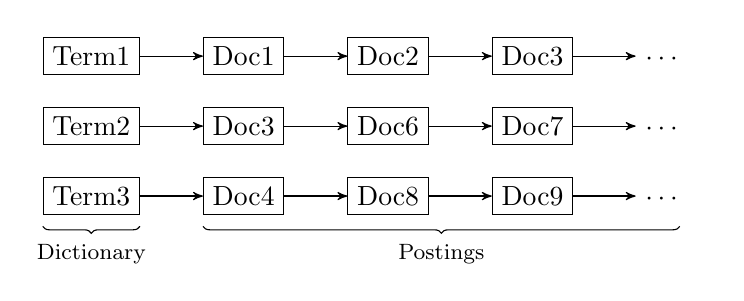
\begin{tikzpicture}
        \matrix (m) [matrix of nodes,nodes={draw},column sep=8mm,row sep=4mm] {
          Term1 & Doc1 & Doc2 & Doc3 & |[draw=none]| $\cdots$\phantom{T} \\
          Term2 & Doc3 & Doc6 & Doc7 & |[draw=none]| $\cdots$\phantom{T} \\
          Term3 & Doc4 & Doc8 & Doc9 & |[draw=none]| $\cdots$\phantom{T} \\
        };
        \draw[->] (m-1-1) -- (m-1-2);
        \draw[->] (m-1-2) -- (m-1-3);
        \draw[->] (m-1-3) -- (m-1-4);
        \draw[->] (m-1-4) -- (m-1-5);
        \draw[->] (m-2-1) -- (m-2-2);
        \draw[->] (m-2-2) -- (m-2-3);
        \draw[->] (m-2-3) -- (m-2-4);
        \draw[->] (m-2-4) -- (m-2-5);
        \draw[->] (m-3-1) -- (m-3-2);
        \draw[->] (m-3-2) -- (m-3-3);
        \draw[->] (m-3-3) -- (m-3-4);
        \draw[->] (m-3-4) -- (m-3-5);
        \draw[decorate,decoration={brace,mirror,raise=4pt}] (m-3-1.south west) -- node[midway,below,yshift=-7pt] {\footnotesize Dictionary} (m-3-1.south east);
        \draw[decorate,decoration={brace,mirror,raise=4pt}] (m-3-2.south west) -- node[midway,below,yshift=-7pt] {\footnotesize Postings} ($(m-3-5.south east) - (1em,0)$);
    \end{tikzpicture}
    \caption{The structure of an inverted index: the dictionary contains terms and the postings contains lists of documents that each term appears in.}
    \label{fig:invertedIndex}
\end{figure}

\section{Introduction to MirageOS}

Running ORAM in the cloud allows a user to access their data from any location. The ORAM client is a trusted cloud instance, and the server is a cloud storage provider, as illustrated in \cref{fig:cloudInstance}.

\begin{figure}
    \centering
    \tikzstyle{principal}=[draw,node distance=50mm,minimum width=30mm,minimum height=25mm,text width=20mm,text centered]
    \begin{tikzpicture}
        \node[principal] (user) {User};
        \node[principal,right of=user] (ci) {Cloud Instance};
        \node[principal,right of=ci] (csp) {Cloud Storage Provider};
        \draw[<->] (user) -- (ci);
        \draw[<->] (ci) -- (csp);
        \draw[decorate,decoration={brace,mirror,raise=4pt}] (ci.south west) -- (csp.south east) node[midway,below,yshift=-4mm] {Path ORAM Protocol};
    \end{tikzpicture}
    \caption{ORAM can be built as a MirageOS application, which can run on a trusted cloud instance.}
    \label{fig:cloudInstance}
\end{figure}

MirageOS is a unikernel operating system. In other words, a MirageOS application is compiled to an executable, along with only the necessary parts of the OS. It can be compiled for a number of targets, including Unix or Xen. An executable, running directly on the Xen hypervisor in the cloud, is more lightweight than the traditional cloud stack, which runs an application on a full operating system, such as Ubuntu. By building ORAM as a MirageOS application, this project allows an instance running ORAM to be spun up whenever the user needs, and shut down when not in use, minimising its cost.

\section{System Architecture}

This project uses the framework illustrated in \cref{fig:cloudInstance}. The focus is on implementing the code for the cloud instance, which consists of the implementation of Path ORAM, a file system running on top of it, and a search module that presents an API to the user. Writing interfaces for specific cloud storage providers is left as future work, so for the purposes of this project a local block device is used for storage.

MirageOS provides an interface for a block device, \texttt{BLOCK}. The ORAM module is designed to satisfy this interface, so that it can be inserted into existing Mirage applications. It is also designed to run on any underlying storage that satisfies \texttt{BLOCK} and, thus, interfaces for cloud storage providers could be written to be compatible with ORAM. The encryption module is designed in the same way, so it can be inserted between ORAM and the underlying storage. \Cref{fig:miragestack} shows the overall structure of the application.

\setlength{\unitlength}{0.75mm}
\begin{figure}[t]
    \centering
    \begin{picture}(170,70)
        \put(50,60){\framebox(50,10){File system}}
        
        \put(100,65){\vector(1,0){20}}
        \put(120,65){\vector(-1,0){20}}
        
        \put(120,60){\framebox(50,10){Search module}}
        
        \multiput(44,55)(4,0){32}{\line(1,0){2}}
        \put(0,54){\texttt{BLOCK} Interface}
        \put(75,60){\vector(0,-1){10}}
        \put(75,50){\vector(0,1){10}}
        
        %\put(145,45){\vector(0,1){15}}
        %\put(145,45){\vector(-1,0){45}}
        
        \put(50,40){\framebox(50,10){ORAM}}
        
        \multiput(44,35)(4,0){32}{\line(1,0){2}}
        \put(0,34){\texttt{BLOCK} Interface}
        \put(75,40){\vector(0,-1){10}}
        \put(75,30){\vector(0,1){10}}
        
        \put(50,20){\framebox(50,10){Encryption}}
        
        \multiput(44,15)(4,0){32}{\line(1,0){2}}
        \put(0,14){\texttt{BLOCK} Interface}
        \put(75,20){\vector(0,-1){10}}
        \put(75,10){\vector(0,1){10}}
        
        \put(50,0){\framebox(50,10){\texttt{BLOCK}}}
    \end{picture}
    \caption{The application stack: ORAM satisfies MirageOS's \emph{\texttt{BLOCK}} interface and any underlying \emph{\texttt{BLOCK}} implementation can be used.}
    \label{fig:miragestack}
\end{figure}
\setlength{\unitlength}{0.5mm}

\section{Requirements Analysis}

\begin{description}
    \item [High Priority] Basic ORAM
    \item [Medium Priority] File system, Search module
    \item [Low Priority] Encryption, Statelessness (Extension), Recursion (Extension)
\end{description}

Building ORAM is the core focus of the project and as such is given high priority. The addition of the file system and search module creates a complete system that can be evaluated, so these two modules are of medium priority. Encryption is necessary in a real world system, but not to perform evaluation, so it is given low priority. Recursion and stateless are extensions, and are therefore deemed to have low priority.

\section{Choice of Tools}

\subsection{OCaml}

OCaml is the logical choice of programming language when building for MirageOS, because Mirage applications and libraries all use OCaml. However, OCaml's module and type systems were also considerations in the choice of Mirage for this project.

OCaml has a powerful module system. It allows one to build \emph{functors}, which are modules parametrised over module interfaces. Any module that satisfies the interface can be given to the functor to create a new concrete module. ORAM can therefore be implemented as a functor that is parametrised over the \texttt{BLOCK} interface.

OCaml's static typing system is an indispensable tool for ensuring the correctness of programs and for increasing productivity.

I had not used OCaml before beginning this project, so learning OCaml and many of its important libraries took a considerable amount of work at the start of the project, and as new libraries were required.

\subsection{Libraries}
\label{subsec:libraries}

The libraries used for building ORAM are listed in \cref{tab:libraries}.

\begin{table}[h]
\centering
\begin{tabularx}{\textwidth}{|l|l|X|l|}
\hline
\textit{Library} & \textit{Version} & \textit{Purpose} & \textit{License} \\
\hline \hline
Mirage & 2.6.1 & System Component Interface Definitions, Application Configuration Framework & ISC \\
\hline
Jane Street's Core & 113.00.00 & Data Structures, Algorithms & Apache-2.0 \\
\hline
LWT & 2.5.1 & Threading & LGPL-2.1 \\
\hline
Cstruct & 1.8.0 & Data Structure & ISC \\
\hline
Alcotest & 0.4.6 & Unit Testing & ISC \\
\hline
Mirage Block CCM & 1.0.0 & Encryption & ISC \\
\hline
Stemmer & 0.2 & Linguistic Processing & GNUv2 \\
\hline
\end{tabularx}
\caption{Libraries used by Mirage ORAM}
\label{tab:libraries}
\end{table}

\subsection{Development Environment}

Choosing the right tools is essential to the productivity of large projects. For OCaml, one of the most important tools is OASIS, which automatically generates Makefiles for a project, based on a specification file. Direct use of the OCaml compiler quickly becomes infeasible when linking together a large number of modules. OASIS deals with this automatically.
Emacs proved incredibly useful, because code indentation, syntax highlighting, autocompletion, and type inspection are all provided by third-party plug-ins. Code can be interpreted, compiled, and run from a shell within Emacs, which boosts productivity.

\begin{table}[t]
    \centering
    \begin{tabular}{|l|l|l|l|}
      \hline
      \textit{Tool} & \textit{Version} & \textit{Purpose} & \textit{License} \\
      \hline \hline
      Mac OSX & 10.11.2 & Operating System & Proprietary \\
      \hline
      Emacs & 24.5 & Text Editor & GPL \\
      \hline
      git & 2.8.0 & Version Control & GPLv2 \\
      \hline
      OPAM & 1.2.2 & Package Manager & GPLv3 \\
      \hline
      OASIS & 0.4.5 & Build Tool & LGPL-2.1 \\
      \hline
    \end{tabular}
    \caption{Tools used in the development of Mirage ORAM}
    \label{tab:devtools}
\end{table}

\section{Software Engineering Techniques}

I employed two key techniques to ensure my code was well-designed and well-built, without compromising productivity.

Firstly, I wrote the interface file for each module before writing the implementation. This forced me to make important design decisions up front, clarifying the structure of the module and its relation to the system as a whole.

Secondly, I practised Test Driven Development \cite{hunt2004pragmatic}. I unit tested each new piece of code as it was written, allowing me to fail fast and fix problems at their source. This approach meant that small modules could be integrated into a larger system that worked as expected more often than not.

Combining these techniques with documentation and structuring of both the source code and the source repository led to a manageable and productive development workflow.

\section{Summary}

This chapter has covered the work undertaken prior to development. This included a definition of the threat model, a brief introduction to the major algorithms, data structures and libraries, an overview of the preliminary architectural design, and a discussion of the techniques and tools selected for the development process.

The next chapter demonstrates how this preparatory material was applied to successfully implement the Path ORAM protocol on MirageOS, and how this protocol was used to build a secure encrypted keyword search application.

\chapter{Implementation}

This chapter explains the process of building a functioning system, using the designs and algorithms of the previous chapter. An overview diagram of the system is given in \cref{fig:systemOverview}. Each module will be examined in turn, working upwards through the diagram. Thus, the chapter begins with a discussion of encryption in \cref{sec:encryption}, followed by a longer discussion of ORAM in \cref{sec:pathORAM}, which constitutes the main focus of the project. This includes subsections about the extensions: recursion and statelessness. Finally, the file system and search modules are explored in \cref{sec:fileSystem,sec:searchmodule} respectively.

The main challenges and achievements of the implementation can be summarised with reference to \cref{fig:systemOverview}.

At the inter-modular level, integration of all parts of the system required careful API design and intricate manipulation of the OCaml module system.

For encryption, an appropriate library had to be chosen, a process that involved filing a pull request to fix a critical bug.

The ORAM module presented the challenge of translating the terse pseudocode of the Path ORAM protocol into a functioning program. This included designing a position map capable of operating on machines of any word size, and building functions to marshal data to and from the format required by ORAM. Adding recursion to this implementation warranted a deeper understanding of the module system, including first class and recursive modules. To achieve statelessness I had to serialise recursive data structures, which meant writing custom functions to conform with a binary protocol.

The implementation of a minimal, but complete, inode-based file system required investigation into the choices made by many file system designers before me. I weighed these against the demands of my system and included only the necessary elements. Furthermore, my file system entailed an implementation of B-Trees, which did not previously exist in OCaml. I therefore implemented a B-Tree library myself that can be applied to other Mirage applications, representing a contribution to the community.

Finally, the search module made use of concepts from the field of Information Retrieval, including algorithms and data structures. The decision to include stemming represented a significant trade-off between the space used by the indexing process and its precision.

\begin{figure}
    \centering
    \tikzstyle{function}=[draw=blue!50,thick,fill=blue!20,minimum width=30mm,minimum height=10mm]
    \tikzstyle{function3high}=[function,minimum height=42.3mm]
    \tikzstyle{function2wide}=[function,minimum width=70mm]
    \tikzstyle{nofunction}=[minimum width=30mm,minimum height=10mm]
    \tikzstyle{data}=[function,draw=red!50,fill=red!20]
    \tikzstyle{module}=[draw,inner sep=0,row sep=6mm,column sep=10mm,ampersand replacement=\&]
    \scalebox{0.9}{
    \begin{tikzpicture}[thick]
        \matrix (search) [module] {
          \node[nofunction] (m00) {Read File}; \&
          \node[nofunction] (m01) {Write File}; \&
          \node[function] (m02) {Search}; \\
          \node[nofunction] (m10) {Read File}; \&
          \node[nofunction] (m11) {Index}; \&
          \node[data] (m12) {Index}; \\
          \node[nofunction] (m20) {Read File}; \&
          \node[nofunction] (m21) {Write File}; \&
          \node[function] (m22) {Flush}; \\
        };
        \node[font=\large] at ($(search) - (75mm,0)$) {Search};
        \node[function3high] (readfile) at ($(m10) + (0.15mm,0)$) {Read File};
        \node[function3high] (writefile) at ($(m11) + (0.15mm,0)$) {Write File};
        \matrix (fs) at ($(search) - (0,55mm)$) [module] {
          \node[nofunction] (m30) {Read File}; \&
          \node[nofunction] (m31) {Write File}; \&
          \node[data] (m32) {Free Map}; \\
          \node[nofunction] (m40) {Read File}; \&
          \node[nofunction] (m41) {Write File}; \&
          \node[data] (m42) {Inode Index}; \\
          \node[nofunction] (m50) {Read}; \&
          \node[nofunction] (m51) {Write}; \&
          \node[function] (m52) {Flush}; \\
        };
        \node[font=\large] at ($(fs) - (75mm,0)$) {File System};
        \node[function3high] at ($(m40) + (0.15mm,0)$) {Read File};
        \node[function3high] at ($(m41) + (0.15mm,0)$) {Write File};
        \matrix (oram) at ($(fs) - (0,55mm)$) [module] {
          \node[function] (m60) {Read}; \&
          \node[function] (m61) {Write}; \&
          \node[data] (m62) {Position Map}; \\
          \node[nofunction] (m70) {Access}; \&
          \node[nofunction] (m71) {Access}; \&
          \node[data] (m72) {Stash}; \\
          \node[function] (m80) {Read Bucket}; \&
          \node[function] (m81) {Write Bucket}; \&
          \node[function] (m82) {Flush}; \\
        };
        \node[font=\large] at ($(oram) - (75mm,0)$) {ORAM};
        \node[function2wide] (funcaccess) at ($(m70) + (20.15mm,0)$) {Access};
        \matrix (enc) at ($(oram) - (0,55mm)$) [module] {
          \node[function] (m90) {Read}; \&
          \node[function] (m91) {Write}; \\
          \node[nofunction] (mA0) {Encrypt}; \&
          \node[nofunction] (mA1) {Encrypt}; \\
          \node[function] (mB0) {Read}; \&
          \node[function] (mB1) {Write}; \\
        };
        \node[font=\large] at ($(enc) - (75mm,0)$) {Encryption};
        \node[function2wide] (funcenc) at ($(mA0) + (20.15mm,0)$) {Encrypt};
        \matrix (disk) at ($(enc) - (0,40mm)$) [module] {
          \node[function] (mC0) {Read}; \&
          \node[function] (mC1) {Write}; \\
        };
        \node[font=\large] at ($(disk) - (75mm,0)$) {Disk};
        \draw[->] ($(m01) + (0,15mm)$) -- (m01);
        \draw[->] (m11) -- (m12);
        \draw[->] (m21) -- (m31);
        \draw[->] (m51) -- (m61);
        \draw[->] (m61) -- (funcaccess);
        \draw[->] (funcaccess) -- (m81);
        \draw[->] (m81) -- (m91);
        \draw[->] (m91) -- (funcenc);
        \draw[->] (funcenc) -- (mB1);
        \draw[->] (mB1) -- (mC1);
        \draw[->] (mC0) -- (mB0);
        \draw[->] (mB0) -- (funcenc);
        \draw[->] (funcenc) -- (m90);
        \draw[->] (m90) -- (m80);
        \draw[->] (m80) -- (funcaccess);
        \draw[->] (funcaccess) -- (m60);
        \draw[->] (m60) -- (m50);
        \draw[->] (m30) -- (m20);
        \draw[->] (m00) -- ($(m00) + (0,15mm)$);
        \draw[->] (m02) -- ($(m02) + (0,15mm)$);
        \draw[->] (m12) -- (m02);
        \draw[->] (m12) -- (m22);
        \draw[->] (m22) -- (m31);
        \draw[<->] ($(m41.east) + (0,2mm)$) -- (m32);
        \draw[<->] (m41) -- (m42);
        \draw[->] (m32) to [bend left=90] (m52);
        \draw[->] (m42) -- (m52);
        \draw[->] (m52) -- (m61);
        \draw[<->] (funcaccess) -- (m62);
        \draw[<->] (funcaccess) -- (m72);
        \draw[->] (m62) to [bend left=90] (m82);
        \draw[->] (m72) -- (m82);
        \draw[->] (m82) -- (m91);
    \end{tikzpicture}}
    \caption{An overview of the system, showing the flow of data. Black boxes are modules, blue are functions, and red are data structures.}
    \label{fig:systemOverview}
\end{figure}

\section{Encryption}
\label{sec:encryption}

ORAM's security depends on the security of the underlying encryption layer. Therefore, it is safer to use a trusted cryptographic library for this task, rather than implementing encryption directly.

Conveniently, the OCaml library Mirage Block CCM creates encrypted block devices that satisfy Mirage's \texttt{BLOCK} interface. It provides a functor, which is a module parametrised over a module interface. This functor takes a module that satisfies the \texttt{BLOCK} interface, and returns a new module, which satisfies the same interface but now uses encryption. ORAM is implemented in the same way, allowing the functors to be chained together to make an encrypted ORAM module.

To create the encrypted block device, and later connect to it, a key must be supplied. While key management would need to be dealt with properly in a real-world system, it is left out of the scope of this project. For the purposes of this project, a constant, known key is used throughout the evaluation.

\begin{listing}[t]
\caption{MirageOS's \texttt{BLOCK} module signature}
\label{lst:blocksig}
\vskip 10pt
\begin{minted}[fontsize=\scriptsize,breaklines]{ocaml}
module type BLOCK = sig

  type page_aligned_buffer = Cstruct.t

  type +'a io = 'a Lwt.t

  type t

  type error = [
    | `Unknown of string (** an undiagnosed error *)
    | `Unimplemented     (** operation not yet implemented in the code *)
    | `Is_read_only      (** you cannot write to a read/only instance *)
    | `Disconnected      (** the device has been previously disconnected *)
  ]

  type id

  val disconnect: t -> unit io

  type info = {
    read_write: bool;    (** True if we can write, false if read/only *)
    sector_size: int;    (** Octets per sector *)
    size_sectors: int64; (** Total sectors per device *)
  }

  val get_info: t -> info io

  val read: t -> int64 -> page_aligned_buffer list -> [ `Error of error | `Ok of unit ] io

  val write: t -> int64 -> page_aligned_buffer list -> [ `Error of error | `Ok of unit ] io

end
\end{minted}
\end{listing}

\section{Path ORAM}
\label{sec:pathORAM}

This section discusses how the abstract data structures and algorithms covered in \cref{sec:oramintro} were realised, and the design decisions involved in the implementation of the Path ORAM protocol.

\subsection{Inherent Constraints}
\label{subsec:constraints}

Writing an implementation to satisfy an existing interface places a number of constraints on the design of the system.

The first constraint is the obligatory use of the Cstruct library, introduced in \cref{subsec:libraries}. \texttt{BLOCK}'s \texttt{read} and \texttt{write} methods both require buffers of type \texttt{Cstruct.t}. ORAM therefore inputs buffers of this type and passes them to the underlying block device. To avoid unnecessary work marshalling data, all data is manipulated in this form.

Another constraint limits the type of addresses in \texttt{BLOCK}'s \texttt{read} and \texttt{write} operations to \texttt{int64}. Again, to avoid unnecessary (and potentially unsafe) work converting between types, \texttt{int64}s are used wherever possible.

\subsection{Stash}
\label{subsec:stashImpl}

The stash stores blocks of data temporarily on the client before they are written back into the tree on the server. It needs to support operations of insertion, lookup based on address, and removal. For this task I chose an \texttt{int64}-keyed hash table from Jane Street's Core library, with \texttt{Cstruct.t} values. The hash table takes constant time for the operations of insertion, lookup and removal, making it ideal for this purpose. This was abstracted into its own module, hiding the underlying type. Thus, the implementation of the stash module can be swapped without breaking the core code of the ORAM module.

The hash table implementation takes an initial size as a parameter, and expands when necessary. Expansion would add a large overhead, because the entire contents of the stash would have to be copied. However, as shown in \citet{stefanov2013path}, for a tree of height $L$ and bucket size $Z$, the stash requires exactly $Z \cdot (L +1)$ blocks of transient storage, and a constant amount of space for persistent storage. Therefore, the hash table should not need to perform expansion at run-time, if it is initialised to a size of at least this constant. \Cref{tab:stashsizes} shows the maximum stash size required, depending on the security parameter, $\lambda$, and the bucket size, $Z$. A stash with security parameter $\lambda$ has probability $2^{-\lambda}$ of exceeding this stash size.

To achieve statelessness, the stash must be written to disk. Increasing the security parameter increases the size of the stash, and therefore the time overhead of statelessness. However, the security parameter must be high enough to ensure long term security. Therefore, a trade-off must be made between security and speed. While keeping the security parameter high, the time overhead can be improved by reducing the size of a block. As mentioned above, there is a constant maximum number of blocks in the stash, so this reduction will have a direct effect on the time taken for each access.

\begin{table}
\centering
\begin{tabular}{|l|l|l|l|}
    \hline
    & \multicolumn{3}{c|}{Bucket Size ($Z$)} \\
    \cline{2-4}
    Security Parameter ($\lambda$) & 4 & 5 & 6 \\
    \cline{2-4}
    & \multicolumn{3}{c|}{Max Stash Size} \\
    \hline
    80 & 89 & 63 & 53 \\
    \hline
    128 & 147 & 105 & 89 \\
    \hline
    256 & 303 & 218 & 186 \\
    \hline
\end{tabular}
\caption{Empirical results for maximum persistent stash size from \citet{stefanov2013path}}
\label{tab:stashsizes}
\end{table}

\subsection{Position Map}

The position map associates a leaf position with each block of the data. As mentioned in \cref{subsec:constraints}, the \texttt{BLOCK} interface constrains the type of block addresses to \texttt{int64}. OCaml provides a Bigarray module, but the size of its arrays is specified using the OCaml \texttt{int} type. This type only uses 63 bits on a 64-bit machine and 31 on a 32-bit machine. Both of these types are also signed, reducing the number of available bits by one. Therefore, a type that can range up to $2^{64} - 1$ needs to be represented using a type that can only go up to $2^{30} - 1$ on a 32-bit machine.

To accommodate this, I built the position map using 3-dimensional arrays. The index, an \texttt{int64} value, is split into a 4-bit value and two 30-bit values. The 4-bit value consists of the four most significant bits, and will therefore have a value of 0 unless more than $2^{60}$ blocks are being stored. The 30-bit values are guaranteed to be converted into non-negative \texttt{int}s, which can then be used to index two dimensions of the array.

In the position map's \texttt{create} function, \Cref{alg:posmapdims} is used to translate from the desired \texttt{int64} size to the dimensions of a 3-dimensional array. After splitting the \texttt{int64} as described above, a value of 1 is added to the first two dimensions to ensure that they are at least of size 1. If a higher dimension is greater than 1, then all lower dimensions become their maximum value, in this case $2^{30}-1$. Using these dimensions, the position map is guaranteed to be at least the size that we require on both 32-bit and 64-bit machines.

\begin{algorithm}[t]
\caption{Calculate the dimensions of a 3D array given total desired size}
\label{alg:posmapdims}
\footnotesize
\begin{algorithmic}[1]
\vskip 10pt
\Require{$\mathsf{size} > 0$}
\vskip 10pt
\Function{PosMapDims}{$\mathsf{size}$}
\vskip 10pt
    \State $(x, y, z) \gets$ \Call{SplitIndices}{$\mathsf{size}$}
\vskip 10pt
    \State $x \gets x + 1$
    \State $y \gets y + 1$
\vskip 10pt
    \If{$x > 1$}
        \State $y \gets \mathsf{0x3FFFFFFF}$
        \State $z \gets \mathsf{0x3FFFFFFF}$
    \ElsIf{$y > 1$}
        \State $z \gets \mathsf{0x3FFFFFFF}$
    \EndIf
\vskip 10pt
    \State \Return $(x,y,z)$
\vskip 10pt
\EndFunction
\vskip 10pt
\end{algorithmic}
\end{algorithm}

\subsection{Creating ORAM}

A major goal of this project was to be build ORAM such that it could replace any existing block device in any Mirage program. To do this, the ORAM module must satisfy MirageOS's \texttt{BLOCK} interface, shown in \cref{lst:blocksig}. It also requires access to the methods of the underlying block device, as well as to the block device itself. ORAM is therefore built as a functor in the same way as the encryption module. This functor takes a module that satisfies the \texttt{BLOCK} interface and returns a new module, which satisfies the same interface, but now implements the Path ORAM protocol.

ORAM's \texttt{create} method takes a block device as input and returns an instance of ORAM, which has the type \texttt{Oram.Make(B).t}, shown in \cref{lst:orammaketype}. This type contains the ORAM parameters, such as \texttt{bucketSize} and \texttt{blockSize}, and  structural information, such as the \texttt{height} of the ORAM and the \texttt{numLeaves}, as well as pointers to the stash, position map, and underlying block device.

Along with the block device, the following parameters are passed as input to the \texttt{create} method:

\begin{description}
  \item[\texttt{size}] The desired size of the ORAM in blocks
  \item[\texttt{blockSize}] The desired size of a single block in bytes
  \item[\texttt{bucketSize}] The number of blocks in a bucket
\end{description}

Using these, the \texttt{create} method can calculate new structural information. The \texttt{BLOCK} interface defines the size of the block device in \emph{sectors}, using the variable \texttt{size\_sectors}, and defines the size of a sector using \texttt{sector\_size}. We will continue to refer to data blocks in ORAM as blocks, but to satisfy \texttt{BLOCK}, ORAM exposes values for both \texttt{size\_sectors} and \texttt{sector\_size}. First, the number of sectors required for a block is calculated as $$\mathtt{sectorsPerBlock} = \frac{\mathtt{blockSize} - 1}{\mathtt{sector\_size}} + 1,$$ which rounds up the number of sectors so the desired block size can always fit. The \texttt{sector\_size} that ORAM uses is the size of the part of the block that stores data. Thus, the size of the address, 8 bytes, is subtracted giving $$\mathtt{sector\_size} = \mathtt{sector\_size} \times \mathtt{sectorsPerBlock} - 8.$$

Now the height of the tree can be calculated, but there are two cases to consider. If the desired size of the ORAM is specified, then the height is calculated as $$L = \left\lfloor \log_2\left(\frac{N}{Z} + 1\right)\right\rfloor - 1.$$ This is obtained by rearranging the equation for the size of the binary tree in buckets, $2^{L + 1} - 1$. The floor operator is introduced, resulting in a binary tree of size less than or equal to the desired size that will definitely fit on the block device. If, instead, the size is unspecified, it is assumed that ORAM should fill as much of the device as possible. The desired size becomes $$N = \frac{\mathtt{size\_sectors}}{\mathtt{sectorsPerBlock}}$$ and then the same calculation as above is performed with this new value. Finally, \texttt{numLeaves} and a new value for \texttt{size\_sectors} are calculated from $L$ using the usual equations for a binary tree.

All of the structural information is now known, so the \texttt{create} method can now create instances of the client-side data structures and initialise the ORAM space. To do the former, it calls the creation functions of the associated data structures. For the latter, it loops through the block device, writing dummy blocks to every location. Dummy blocks have address $-1$, and are ignored by the access protocol. Finally, the \texttt{create} method packages everything up as an instance of \texttt{ORAM.Make(B).t}.

\begin{listing}[t]
\caption{The type of an ORAM device \texttt{ORAM.Make(B).t}}
\label{lst:orammaketype}
\inputminted[fontsize=\scriptsize,firstline=87, lastline=118]{ocaml}{../mirage-oram/lib/oram.ml}
\end{listing}

\subsection{Accessing ORAM}

The main logic of ORAM resides in the \texttt{access} function, the implementation of \cref{alg:access}. Before discussing this, it is worth mentioning the plumbing that occurs on either side of it. The \texttt{BLOCK} interface function \texttt{write} inputs data as a list of \texttt{Cstruct.t}s with no defined size. The \texttt{access} function expects a fixed-sized block tagged with an address, so \texttt{write} splits the input into chunks and tags them, before calling \texttt{access} on each one.

The subroutines \texttt{readBucket} and \texttt{writeBucket} are on the other side of \texttt{access}. They are responsible for communicating with the underlying block device and, more importantly, maintaining the structure of the logical binary tree. There are no physical pointers, but instead the structure is built by calculating the appropriate physical address of a bucket. The physical address of the bucket on the path to leaf $x$ at level $l$ is calculated using \cref{alg:bucketaddress}.

\begin{algorithm}[t]
  \footnotesize
  \begin{algorithmic}
  \vskip 10pt
    \Function{BucketAddress}{$x$,$l$}
      \State $address \gets 0$
      \For{$i = 0;~i < l;~i++$}
        \If{$x >> (i + \mathtt{height} - l)~\&\&~1 = 1$}
          \State $address \gets (2 \times address) + (\mathtt{bucketSize} \times \mathtt{sectorsPerBlock} \times 2)$
        \Else
          \State $address \gets (2 \times address) + (\mathtt{bucketSize} \times \mathtt{sectorsPerBlock})$
        \EndIf
      \EndFor
      \State \Return $address$
    \EndFunction
  \vskip 10pt
  \end{algorithmic}
  \caption{Calculating the physical address of the bucket at level $l$ on the path to leaf $x$}
  \label{alg:bucketaddress}
\end{algorithm}

\begin{figure}[t]
    \centering
    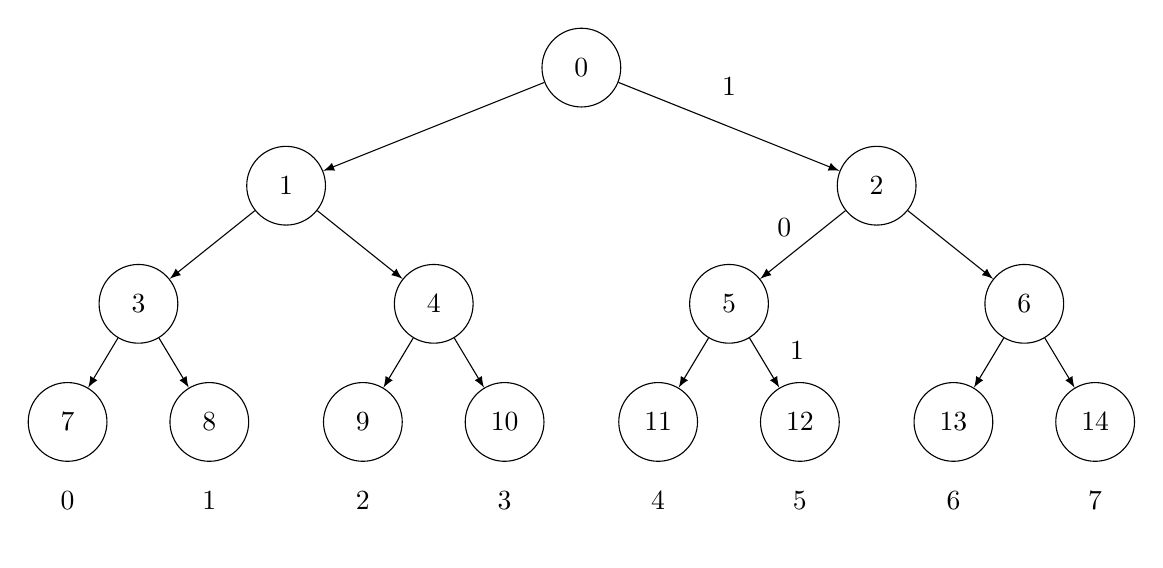
\begin{tikzpicture}[level/.style={sibling distance=75mm/#1},
        level 3/.style={sibling distance=18mm},
        every node/.style={minimum size=10mm,shape=circle},
        edge from parent/.style={draw,-latex}]
        \node[draw,grow=down] {0}
        child {
          node[draw] {1}
          child { node[draw] {3}
            child {
              node[draw] (n7) {7}
            }
            child { node[draw] (n8) {8} }
          }
          child { node[draw] {4}
            child { node[draw] (n9) {9} }
            child { node[draw] (n10) {10} }
          }
        }
        child {
          node[draw] {2}
          child { node[draw] {5}
            child { node[draw] (n11) {11} }
            child {
              node[draw] (n12) {12}
              edge from parent node[near start,right] {1}
            }
            edge from parent node[near start,left] {0}
          }
          child { node[draw] {6}
            child { node[draw] (n13) {13} }
            child { node[draw] (n14) {14} }
          }
          edge from parent node[above] {1}
        };
        \node [below of=n7] {0};
        \node [below of=n8] {1};
        \node [below of=n9] {2};
        \node [below of=n10] {3};
        \node [below of=n11] {4};
        \node [below of=n12] {5};
        \node [below of=n13] {6};
        \node [below of=n14] {7};
  \end{tikzpicture}
  \caption{Visualisation of \cref{alg:bucketaddress}}
  \label{fig:bucketaddress}
\end{figure}

This is most easily explained using \cref{fig:bucketaddress}. Here, the nodes are labelled in order of their position in memory. The leaves are also labelled, but the binary representations of these labels are more important. The binary representation of leaf $x$, read from left to right, denotes the set of operations required to calculate the physical address of $x$. A 0 denotes taking the left branch at a node, labelled $n$, and the resulting node has label $2n + 1$. A 1 denotes taking the right branch, and the resulting node has label $2n+2$. For example, the path to leaf 5, with binary representation 101, takes the right branch from the root, then the left branch, and then the right, giving $$2 \cdot (2 \cdot (2 \cdot 0 + 2) + 1) + 2 = 12.$$ Multiplying this node label by the block size and the bucket size gives the physical address of the node. The same procedure can be used for a node at a specific level, $l$, but now only the path denoted by the first $l$ bits will be followed.

The final part of ORAM is the \texttt{access} function. Its parameters are \texttt{op}, which is either \texttt{read} or \texttt{write}, \texttt{a}, which is the address of the block to access, and \texttt{data'}, which contains the data to be written when \texttt{op} is \texttt{write}. \texttt{data'} is implemented using an option type, so when \texttt{op} is \texttt{read}, \texttt{data'} will have value \texttt{None}.

In \cref{sec:oramintro}, \texttt{access} was split into four steps:
\begin{enumerate}
    \item Remap the address, \texttt{a}, in the position map,
    \item Read the path that \texttt{a} was previously mapped to,
    \item If \texttt{op} is \texttt{write}, then write \texttt{data'} into the block with address \texttt{a} in the stash,
    \item Write the same path back, but filled with new blocks from the stash.
\end{enumerate}

Step 1 calls a pseudo-random function to choose a new position for the block uniformly at random. This operation ensures the security of the Path ORAM construction by making subsequent accesses to the same address statistically independent.

Step 2 calculates the physical address for each bucket along the path, using the subroutines described above, then reads the contents of each bucket into the stash.

Step 3 looks up the block with address \texttt{a} in the stash, stores its current data to be returned by the function, and then replaces it with \texttt{data'}.

Step 4 decides which blocks to write back into the path. The na\"ive implementation of this, suggested by \cref{alg:access}, loops through the stash and finds blocks with address \texttt{a'}, such that the bucket at level $l$ on the path to leaf $\mathtt{position[a']}$ is the same as the bucket at level $l$ on the path to leaf $x$. I made two optimisations to this implementation. The first is to perform the position lookup only once, tagging blocks with their positions in a temporary data structure to avoid repeated work at each level. The second is to avoid calculating the bucket addresses entirely; in order for the paths to two leaves to intersect at level $l$, the leaves must have the same first $l$ bits. Thus, checking for intersection can be reduced to performing a right bit shift on both $x$ and $\mathtt{position[a']}$ of $\mathtt{height} - l$ bits, and checking for equality.

This concludes the discussion of the basic ORAM functor, which can be used to augment a block device in any Mirage program. \cref{subsec:recursion,subsec:statelessness} examine the addition of recursion and statelessness to this ORAM construction.

\subsection{Recursion}
\label{subsec:recursion}

The essence of recursive ORAM is that the position map of one ORAM is another ORAM. To make this possible, I extended the original ORAM functor, parametrising it in a new \texttt{PositionMap} interface. This interface is satisfied by the original, in-memory position map module, as well as by the ORAM functor itself. Applying this new ORAM functor once with the in-memory position map module gives the basic ORAM functor discussed above. However, applying the functor again, with the result of the first application, gives a recursive ORAM module with one level of recursion. This can be repeated to an arbitrary depth. This exhibits the power of OCaml's module system.

The recursive ORAM module can be constructed manually as above, applying the functor $n + 1$ times for $n$ levels of recursion. However, it is preferable to build the recursive module automatically, based on the size of the data ORAM, ORAM$_0$. Addresses are 64-bit integers, so they occupy 8 bytes of storage each. If ORAM$_0$ has size $N$ in blocks, and the size of each block is $B$ bytes, then one block in ORAM$_1$, used as the position map for ORAM$_0$, can store $\chi = B / 8$ addresses. The number of blocks required for ORAM$_1$ will therefore be $N / \chi$. After $\log N / \log \chi$ levels of recursion, the in-memory position map will be of size $O(1)$.

So, the recursive ORAM module is created by taking in the size, $N$, and the block size, $B$, and automatically applying the ORAM functor recursively $\log N / \log \chi$ times. Calling the $\mathtt{create}$ function of the resulting module creates ORAM instances with the correct number of levels of recursion.

\subsection{Statelessness}
\label{subsec:statelessness}

In order to achieve statelessness for ORAM, its type information, the stash, and the position map must all be stored on disk. The layout of this information on disk is explained first, followed by the method for flushing it to disk.

Once ORAM has been initialised and is in use, relocating it on disk is very costly, because the whole data structure would need to be copied. However, to reconnect to ORAM, the information necessary to discover ORAM's existence must be stored in a well-known location. The first block of the underlying block device is therefore used as a \emph{superblock}, which is a block containing the most important metadata. This superblock contains a pointer to the location of the rest of the state, along with its length. This way, ORAM can be stored, starting at the second location on disk, and the state can be appended at the end of the ORAM section. Thus, ORAM never has to be moved once it has been initialised.

To store the state, it must be serialised first, which translates it into a form that can be written to disk. For the majority of the information, an existing serialisation library, Jane Street's Bin\_prot, can be used. This is a binary protocol which allows one to annotate a type with \texttt{[@@ deriving bin\_io]} and generates functions to read and write instances of the type into buffers. This is used for all of ORAM's type information, as well as for the stash, but not for the position map. ORAM's type is therefore split into a core, that can use Bin\_prot, and an extended type, which includes the position map and the underlying block device. This structure is shown in \cref{lst:orammaketype} on \cpageref{lst:orammaketype}.

The position map is more difficult to serialise because, under recursive ORAM, it might be another ORAM. To avoid writing the entire position map ORAM onto the disk a second time, a custom serialisation function is used that only stores metadata for ORAM position maps, but stores the entire in-memory position map in the base case. The state is stored at the end of the block device, after all recursive instances, so this function collects the data from all the levels of recursion together into one buffer.

After all the state has been flushed to disk, it is safe to disconnect from ORAM. Reconnecting to ORAM is a case of checking for the presence of the superblock, reading in the location and length of the state, reading the actual state, and then calling the connect function on the position map. The connect function allows each recursive ORAM instance to have its own reference to the underlying block device, and returns once it reaches the in-memory position map.

\section{File System}
\label{sec:fileSystem}

To search over a set of documents, they first need to be stored. A suitable file system for MirageOS did not exist, hence, this section describes the design and implementation of a basic file system that satisfies the requirements of the project.

\subsection{General Design}
The most common way of building a file system on top of a block device is through the use of \emph{inodes}. An inode contains meta-information about a file, along with pointers to the actual data blocks. For the purposes of this project, an inode will simply be one block of the block device, containing the length of the file, followed by the list of pointers. In a system with more complex needs, the inode would contain more information, such as modification/access timestamps, file permissions, etc., but for this project it suffices to be able to read and write documents.

To allow quick access to the inode for a particular file, its location is stored in an index. Rather than indexing based on filenames, which may have variable lengths, it is preferable to index based on the hash of the filename. This allows a more regular layout of the data in memory due to the constant length of indexes. In a real system, collisions in the hash function would need to be handled but, for a small number of files, this possibility can be neglected. \Cref{subsec:inodeindex} describes the implementation of the inode index.

Space needs to be allocated on the block device for inode index blocks, for inode blocks, and for data blocks, which can be achieved using a \emph{free map}. This is a map that tracks whether each block has been allocated and can be updated as new blocks are allocated and freed. \Cref{subsec:freemap} describes the implementation of the free map.

To be able to disconnect from the file system, it needs to be stateless. Therefore, the data structures need to be stored on disk, along with enough information to find them. The root address of the inode index and the length of the free map are enough to locate the data structures on disk when reconnecting to the block device. These two pieces of information are stored at address 0 in another superblock.

\subsection{Inode Index}
\label{subsec:inodeindex}

The inode index associates keys, in the form of filename hashes, with values, in the form of pointers to inodes. It is implemented using B-Trees\footnote{The algorithms for B-Tree operations were adapted from \citet{CLRS09}}, which not only support operations of insertion, lookup, and deletion efficiently, but are also stored directly on disk. There were no B-Tree libraries available for OCaml at the time of writing, so I implemented one myself.

B-Trees are a generalisation of self-balancing binary search trees, where each node can have more than one child. If a node has $n$ children, then it stores $n-1$ keys. It is guaranteed that $$ \forall m \leq n, k \in child_m, j \in child_{m+1} . k < key_m < j,$$ that is, a key is greater than all the keys to its left and less than all the keys to its right.

B-Trees are an efficient on-disk data structure because a whole block can be used for one node. This gives an extremely high branching factor, reducing the depth of the tree and therefore the number of blocks that need to be accessed in any single operation. On creation of the file system, the branching factor of the tree is calculated such that as much of each block as possible is filled with useful information.

I implemented B-Trees as a functor, which is parametrised in three module interfaces: one for the nodes, one for the allocation module, and one for the storage module. This makes the library more generalised, which means it may find wider use in the OCaml community. For the purposes of this project, I wrote a node module that uses 16-bit pointers between nodes, and stores \texttt{int64} inode pointers. For the allocation and the storage modules, this project uses the free map, described in \cref{subsec:freemap}, and the ORAM module, respectively.

\subsection{Free Map}
\label{subsec:freemap}

To allocate space efficiently, an array of bits the size of the block device can be used. For statelessness, the free map is flushed to disk regularly. Therefore, it was beneficial to write my own bit array based on \texttt{Cstruct}s, rather than using a library implementation. This allows the whole structure to be written directly onto the disk using the block device methods, without any costly translation.

The \texttt{Cstruct} library performs data access in bytes. This leads to \cref{alg:bitgetset} for getting and setting individual bits. To get the $n^{th}$ bit, it must be extracted from the $\frac{n}{8}^{th}$ byte. To do this, the index of the bit in the byte is calculated, a 1 is left-shifted to that position, and an and operation is performed, which masks that bit. Setting is a similar operation, but seeks to preserve the surrounding bits. To set a 1, the index of the bit in the byte is calculated, a 1 is shifted to that position, and an or operation is performed, which sets the bit to 1 while preserving all other bits. Setting a 0 is slightly trickier. It would be performed by an and operation with a bit string that is 0 at the desired position and 1 everywhere else, but shifting fills empty bits with 0s. Instead, by the use of De Morgan's Law $$ a~\&\&~b = \neg (\neg a~||~\neg b) $$ this is converted into an operation involving a bit string that has a 1 at the desired position and 0s everywhere else.

\begin{algorithm}[t]
\caption{Getting and setting individual bits in a byte array}
\label{alg:bitgetset}
\begin{algorithmic}
\vskip 10pt
\Function{GetBit}{$\mathsf{index}$}
  \State $byte \gets \mathsf{byteArray[index]}$
  \State $shift \gets 7 - \mathsf{index} \bmod 8$
  \State \Return $byte >> shift~\&\&~1$
\EndFunction
\vskip 10pt
\Function{SetBit}{$\mathsf{index,boolean}$}
  \State $byte \gets \mathsf{byteArray[index]}$
  \State $shift \gets 7 - \mathsf{index} \bmod 8$
  \If{$\mathsf{boolean}$}
    \State $byte \gets byte~||~1 << shift$
  \Else
    \State $byte \gets \neg (\neg byte~||~1 << shift)$
  \EndIf
  \State $\mathsf{byteArray[index]} \gets byte$
\EndFunction
\vskip 10pt
\end{algorithmic}
\end{algorithm}

\section{Search Module}
\label{sec:searchmodule}

The final part of the system performs search over the encrypted documents stored in ORAM. \cref{subsec:invertedindex} discusses building an inverted index, the data structure that enables efficient search. \cref{subsec:searchapi} then explains the front-end of the whole application, the search API.

\subsection{Inverted Index}
\label{subsec:invertedindex}

The basics of inverted indexes are discussed in \cref{sec:invertedindexintro}. As stated, the index consists of two main structures, the dictionary and the postings. For the dictionary, I used the most common implementation, a hash table. This provides $O(1)$ lookup and insertion, which are the main operations required. The postings are more flexible. These are where the filenames are stored, because they are not actually stored in the file system itself. Performing conjunctive queries requires taking the intersection of postings lists. Thus, each postings list is implemented using a hash set, which is a data structure built on top of a hash table. It stores a set of keys, in this case filenames, and has the added benefit of keeping them unique automatically.

As usual in this project, files are stored as \texttt{Cstruct}s. There are a number of steps to be performed in order to index a file. First, the file is converted to a string and immediately stripped of unnecessary characters, including all punctuation. At this point, the file is a sequence of alphanumeric character strings, separated by spaces and newlines, so performing a split on these characters results in a list of words.

Before inserting this list into the index, two techniques are used to improve efficiency. Storing separate words for `run', `ran', and `runs' increases the size of the index. To reduce the impact of this, some linguistic preprocessing is performed. Specifically, stemming is carried out, which uses a set of rules to prune suffixes, mapping words onto a stem. I used a small open-source library implementation of Porter's stemming algorithm \cite{porter1980algorithm}, ocaml-stemmer. This technique not only reduces the size of the index, but also arguably improves search, because now queries for `run' can automatically return documents containing morphological derivations. A second technique removes duplicates from the resulting list of words, reducing insertion overhead. After these techniques have been applied, the remaining entries are inserted into the index.

For the purposes of this project, only simple conjunctive queries are used, meaning search looks for documents containing all of the words in a space-separated query string. To do this, preprocessing is performed as above on the query string. Then, each term is looked up in the dictionary, resulting in a list of hash sets. Finally, the big intersection of these hash sets produces the result. In order to make this intersection operation efficient, the list is first sorted by hash set size. For each pairwise intersection, the smaller hash set is filtered by checking for membership in the larger hash set. This means that one constant time lookup is performed for each member of the small set, rather than the large, resulting in a significant performance boost, as the size of the smaller set is monotonically decreasing.

\subsection{Keyword Search API}
\label{subsec:searchapi}

The final step in an end-to-end system is the API. File system access, indexing and search all need to be wrapped together into one module that provides a single point of entry for the encrypted search system.

There are three main operations which are the most important to support: writing files, reading files, and searching over files. This project is not concerned with deleting files, because this is not necessary for the evaluation of ORAM.

Writing files is the most complicated step because this is where indexing is performed. During a write, the file is first written through to the file system. It is then indexed and, finally, the index is flushed to disk to ensure it persists. Reading files passes through to the file system and search makes calls to the inverted index.

\section{Summary}
\label{sec:implSummary}

In this chapter I have discussed the implementation of all of the components of my system, including the key design decisions and trade-offs that were made. I demonstrated how I implemented recursive Path ORAM in a way that allows it to plug into existing MirageOS programs, and how I built a file system and search operations on top of it.

The next section discusses evaluation, which assesses whether I have implemented ORAM such that it provides functionality, performance, and security and therefore whether the aims of the project have been achieved.

\chapter{Evaluation}

This chapter explains the methodology used to ensure the correctness of the ORAM implementation, and analyses its performance and security properties. \Cref{sec:unitTests} discusses functional testing through the use of unit testing and randomised testing. \Cref{sec:performanceTesting} then goes on to discuss performance, and then finally \cref{sec:statisticalAnalysis} analyses the security of ORAM.

Overall, ORAM performs as expected in terms of functionality, performance, and security. It operates correctly, writing files and reading the same data back out. It continues to do so with the additions of statelessness, recursion, and encryption. All parts of the system are fully functioning, both separately, and as a whole. In terms of performance, my implementation agrees with the theoretical bounds given in \citet{stefanov2013path}, which state $O(\log N)$ time overhead. Finally, statistical analysis shows that ORAM does indeed have a statistically random access pattern, ensuring the security of the implementation.

\section{Unit Tests}
\label{sec:unitTests}

I used unit testing throughout the development process, which allowed me to be sure that individual components were functioning correctly before I combined them into larger, more complicated systems. This section describes the most important test cases that I ran for each module, and discusses the use of randomised testing to cover a larger range of input values. Code coverage testing was also used to make sure that the tests were exercising all parts of the system.

\subsection{Stash}

The three main tests for the stash check that:

\begin{itemize}
  \item Values not expected to be in the stash are not found
  \item Values that have been added to the stash are found
  \item Adding dummy blocks to the stash has no effect
\end{itemize}

During the development process, I hand-coded a small number of example cases. Later, in order to test more extensively, I coded the above three cases as properties for randomised testing. Randomised testing generates a number of test cases and verifies that the properties hold in every case, allowing far more cases to be covered than hand-coded tests alone.

\subsection{Position Map}

Two main aspects of the position map need to be tested. Firstly, the translation of 64-bit addresses into three integer indexes, and, secondly, its operation as a data structure.

The code performing the translation is essentially a mathematical definition in itself, so any property definition that might be used for randomised testing would be equivalent to the original code. Thus, in this instance, a few hand-chosen random cases can be checked, along with the key edge cases. The edge cases to check are the maximum and minimum values, along with values either side of a change in the higher indices. That is, values with output $(x,y,max\_int)$ and $(x,y+1,0)$, and similarly for the higher index.

In terms of operation, it is necessary to check that after adding a value to the position map, the same value is read back, and, furthermore, that trying to add a value at an address outside of the allowed range results in an error. Both of these cases can be coded up as properties for randomised testing.

\subsection{ORAM}

The ORAM implementation is particularly amenable to randomised testing because there are inverse functions for most of its functionality. It is therefore possible to write properties for randomised testing of the form $f(f^{-1}(x)) = x$. This allows each stage of ORAM to be tested independently, from writing individual blocks, through writing whole paths, to writing entire files.

Regular unit testing was performed on other functions, for which properties could not be easily coded. These functions include reconnecting to ORAM to test statelessness, and performing calculations, such as computing the height for ORAM tree.

\subsection{Free Map}

The free map allocates blocks in the block device to be used by different parts of the file system. It is necessary to test that, on creation, the map allocates the correct number of initial blocks, that it always allocates the correct number of blocks if they are available, and that it only ever allocates blocks that are actually free.

During development, I used a selection of test cases which covered important edge cases. These included creating the map, and checking that nothing was allocated to begin with, except the first $n$ blocks, where $n$ is a parameter of the creation function. Then, I tested that allocating and deallocating different sequences of blocks led to the expected results. Finally, I checked that an error was returned if there were not enough free blocks.

After main development was completed, I added some randomised testing to this module to cover a wider range of inputs.

\subsection{B-Trees}

It is not possible to test the B-Tree library directly because it only provides a functor to create a B-Tree. Hence, I tested the B-Tree using the inode index, the canonical use case of the library in this system. In order to test the B-Tree properly, I used randomised testing to create a reasonable access pattern that was guaranteed to cause splitting of the root node.

\subsection{Inodes}

The inodes were tested to make sure they  added and deleted pointers, while maintaining a correct count. Again, this is amenable to randomised testing, although unit tests were also used throughout the development to test specific cases that would be expected to cause exceptions.

\subsection{File System}

To test the file system, I created a large number of random files and used randomised testing to ensure that the correct files were always read back out once they had been written in, under any access pattern. This also included testing to ensure that reasonable exceptions were produced when the file system became full, or a file did not exist in the system.

\subsection{Search Module}

The search module was tested for correctness, i.e. that if a file containing a word had been put into the system, then it would appear in the search results for that word. This was difficult to randomise, so I manually constructed a number of test scenarios.

\section{Performance Testing}
\label{sec:performanceTesting}

\subsection{Parameter Optimisation}
\label{sub:parameterOptimisation}

Before performing the main experiments, I decided to optimise ORAM's parameters so that the experiments could run faster. The main parameter in question is the block size, shown in \citet{ousterhout1985trace} to dramatically affect the speed of IO operations. I discovered that this is indeed the case with ORAM, as can be seen in \cref{fig:blockSizeResults}. It appears that increasing the block size results in an unbounded increase in performance, but I settled on a block size of 1MB to trade off between speed and precision in specifying the size of the block device.

It is important to note that using ORAM in the cloud would give very different results. Increasing the block size would increase the size of the stash proportionally, because the maximum stash size is a constant number of blocks. Thus, a larger block size increases the amount of data that must be written to disk to achieve statelessness. I have shown that increasing block size increases speed on a local disk, but network latency and bandwidth will dominate when running in the cloud, leading to a slow down. I would need to perform further experiments in the cloud to discover an optimal trade-off point for this scenario.

\begin{figure}
    \centering
    %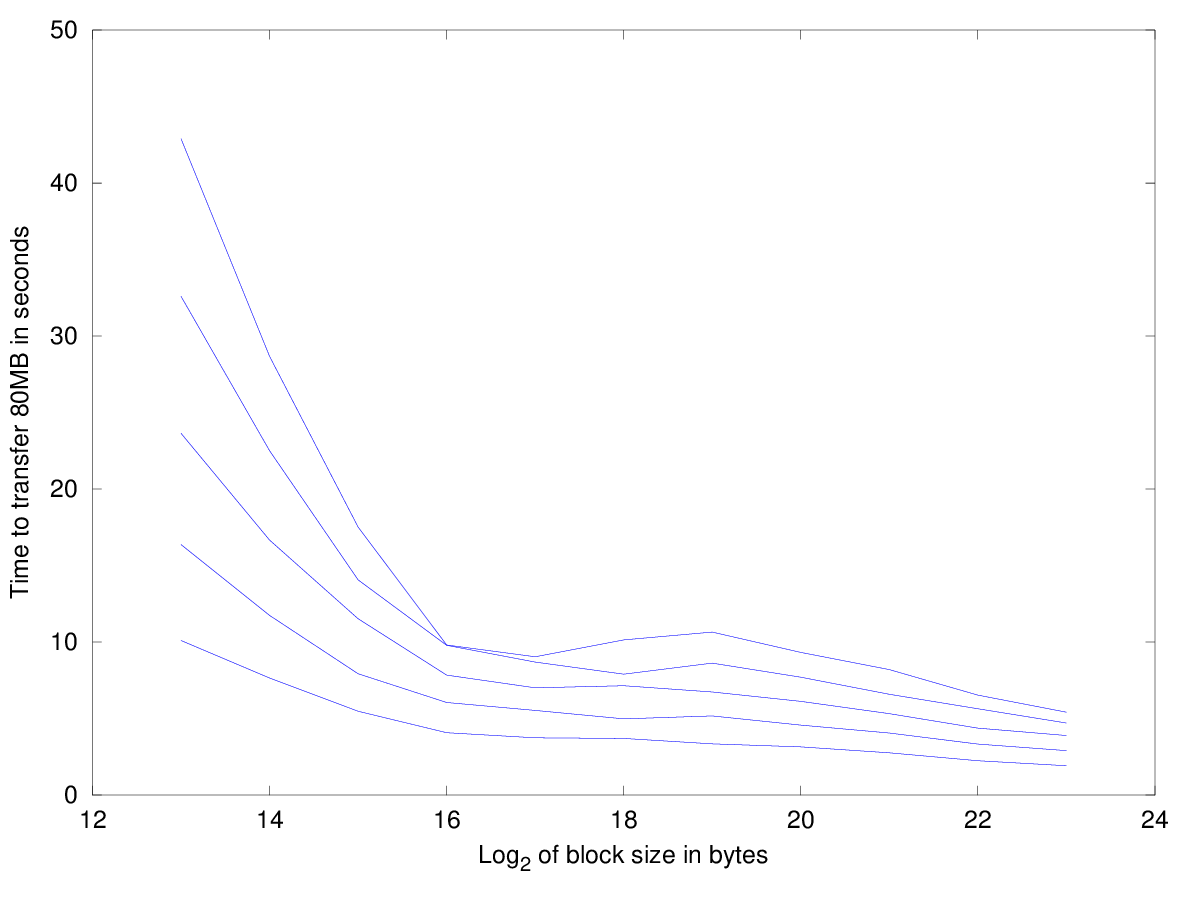
\includegraphics[width=.8\linewidth]{blockSizeResults}
    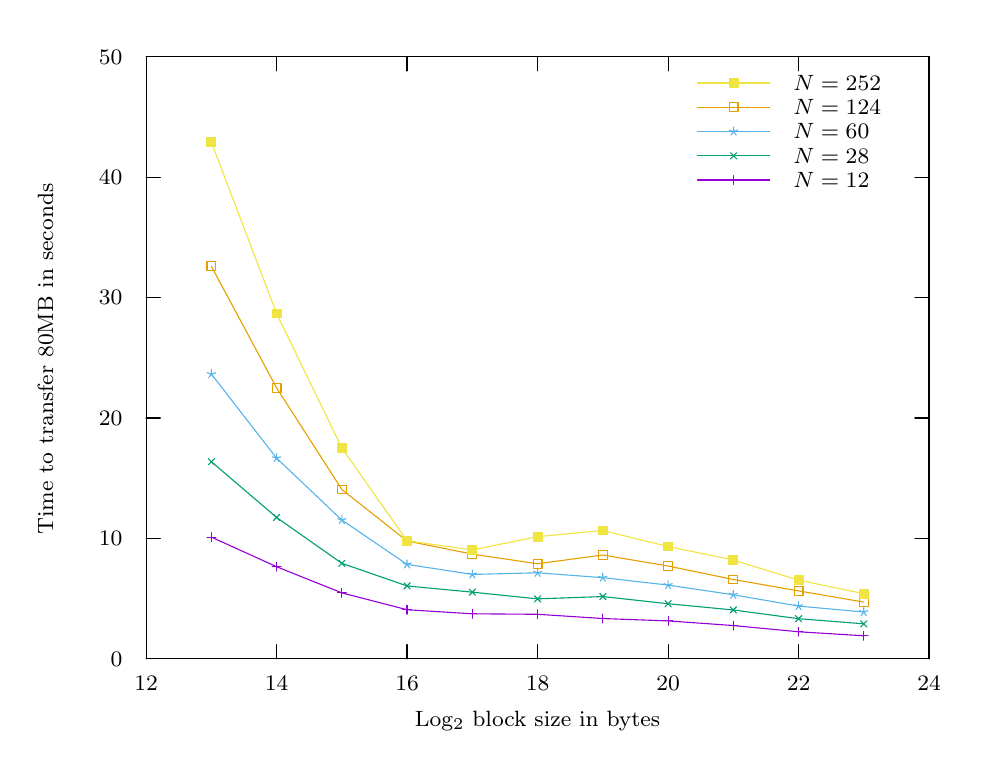
\begin{tikzpicture}[gnuplot]
%% generated with GNUPLOT 5.0p3 (Lua 5.3; terminal rev. 99, script rev. 100)
%% Mon 02 May 2016 09:35:28 BST
\path (0.000,0.000) rectangle (12.000,9.000);
\gpcolor{color=gp lt color border}
\gpsetlinetype{gp lt border}
\gpsetdashtype{gp dt solid}
\gpsetlinewidth{1.00}
\draw[gp path] (1.504,0.985)--(1.684,0.985);
\draw[gp path] (11.447,0.985)--(11.267,0.985);
\node[gp node right] at (1.320,0.985) {\footnotesize 0};
\draw[gp path] (1.504,2.514)--(1.684,2.514);
\draw[gp path] (11.447,2.514)--(11.267,2.514);
\node[gp node right] at (1.320,2.514) {\footnotesize 10};
\draw[gp path] (1.504,4.043)--(1.684,4.043);
\draw[gp path] (11.447,4.043)--(11.267,4.043);
\node[gp node right] at (1.320,4.043) {\footnotesize 20};
\draw[gp path] (1.504,5.573)--(1.684,5.573);
\draw[gp path] (11.447,5.573)--(11.267,5.573);
\node[gp node right] at (1.320,5.573) {\footnotesize 30};
\draw[gp path] (1.504,7.102)--(1.684,7.102);
\draw[gp path] (11.447,7.102)--(11.267,7.102);
\node[gp node right] at (1.320,7.102) {\footnotesize 40};
\draw[gp path] (1.504,8.631)--(1.684,8.631);
\draw[gp path] (11.447,8.631)--(11.267,8.631);
\node[gp node right] at (1.320,8.631) {\footnotesize 50};
\draw[gp path] (1.504,0.985)--(1.504,1.165);
\draw[gp path] (1.504,8.631)--(1.504,8.451);
\node[gp node center] at (1.504,0.677) {\footnotesize 12};
\draw[gp path] (3.161,0.985)--(3.161,1.165);
\draw[gp path] (3.161,8.631)--(3.161,8.451);
\node[gp node center] at (3.161,0.677) {\footnotesize 14};
\draw[gp path] (4.818,0.985)--(4.818,1.165);
\draw[gp path] (4.818,8.631)--(4.818,8.451);
\node[gp node center] at (4.818,0.677) {\footnotesize 16};
\draw[gp path] (6.476,0.985)--(6.476,1.165);
\draw[gp path] (6.476,8.631)--(6.476,8.451);
\node[gp node center] at (6.476,0.677) {\footnotesize 18};
\draw[gp path] (8.133,0.985)--(8.133,1.165);
\draw[gp path] (8.133,8.631)--(8.133,8.451);
\node[gp node center] at (8.133,0.677) {\footnotesize 20};
\draw[gp path] (9.790,0.985)--(9.790,1.165);
\draw[gp path] (9.790,8.631)--(9.790,8.451);
\node[gp node center] at (9.790,0.677) {\footnotesize 22};
\draw[gp path] (11.447,0.985)--(11.447,1.165);
\draw[gp path] (11.447,8.631)--(11.447,8.451);
\node[gp node center] at (11.447,0.677) {\footnotesize 24};
\draw[gp path] (1.504,8.631)--(1.504,0.985)--(11.447,0.985)--(11.447,8.631)--cycle;
\node[gp node center,rotate=-270] at (0.246,4.808) {\footnotesize Time to transfer 80MB in seconds};
\node[gp node center] at (6.475,0.215) {\footnotesize Log$_2$ block size in bytes};
\node[gp node left] at (9.607,7.065) {\footnotesize $N = 12$};
\gpcolor{rgb color={0.580,0.000,0.827}}
\draw[gp path] (8.507,7.065)--(9.423,7.065);
\draw[gp path] (2.333,2.530)--(3.161,2.154)--(3.990,1.822)--(4.818,1.608)--(5.647,1.556)%
  --(6.476,1.550)--(7.304,1.496)--(8.133,1.466)--(8.961,1.407)--(9.790,1.328)--(10.618,1.277);
\gpsetpointsize{4.00}
\gppoint{gp mark 1}{(2.333,2.530)}
\gppoint{gp mark 1}{(3.161,2.154)}
\gppoint{gp mark 1}{(3.990,1.822)}
\gppoint{gp mark 1}{(4.818,1.608)}
\gppoint{gp mark 1}{(5.647,1.556)}
\gppoint{gp mark 1}{(6.476,1.550)}
\gppoint{gp mark 1}{(7.304,1.496)}
\gppoint{gp mark 1}{(8.133,1.466)}
\gppoint{gp mark 1}{(8.961,1.407)}
\gppoint{gp mark 1}{(9.790,1.328)}
\gppoint{gp mark 1}{(10.618,1.277)}
\gppoint{gp mark 1}{(8.965,7.065)}
\gpcolor{color=gp lt color border}
\node[gp node left] at (9.607,7.373) {\footnotesize $N = 28$};
\gpcolor{rgb color={0.000,0.620,0.451}}
\draw[gp path] (8.507,7.373)--(9.423,7.373);
\draw[gp path] (2.333,3.488)--(3.161,2.780)--(3.990,2.197)--(4.818,1.910)--(5.647,1.831)%
  --(6.476,1.746)--(7.304,1.775)--(8.133,1.684)--(8.961,1.605)--(9.790,1.494)--(10.618,1.429);
\gppoint{gp mark 2}{(2.333,3.488)}
\gppoint{gp mark 2}{(3.161,2.780)}
\gppoint{gp mark 2}{(3.990,2.197)}
\gppoint{gp mark 2}{(4.818,1.910)}
\gppoint{gp mark 2}{(5.647,1.831)}
\gppoint{gp mark 2}{(6.476,1.746)}
\gppoint{gp mark 2}{(7.304,1.775)}
\gppoint{gp mark 2}{(8.133,1.684)}
\gppoint{gp mark 2}{(8.961,1.605)}
\gppoint{gp mark 2}{(9.790,1.494)}
\gppoint{gp mark 2}{(10.618,1.429)}
\gppoint{gp mark 2}{(8.965,7.373)}
\gpcolor{color=gp lt color border}
\node[gp node left] at (9.607,7.681) {\footnotesize $N = 60$};
\gpcolor{rgb color={0.337,0.706,0.914}}
\draw[gp path] (8.507,7.681)--(9.423,7.681);
\draw[gp path] (2.333,4.601)--(3.161,3.533)--(3.990,2.747)--(4.818,2.184)--(5.647,2.056)%
  --(6.476,2.077)--(7.304,2.015)--(8.133,1.921)--(8.961,1.798)--(9.790,1.654)--(10.618,1.579);
\gppoint{gp mark 3}{(2.333,4.601)}
\gppoint{gp mark 3}{(3.161,3.533)}
\gppoint{gp mark 3}{(3.990,2.747)}
\gppoint{gp mark 3}{(4.818,2.184)}
\gppoint{gp mark 3}{(5.647,2.056)}
\gppoint{gp mark 3}{(6.476,2.077)}
\gppoint{gp mark 3}{(7.304,2.015)}
\gppoint{gp mark 3}{(8.133,1.921)}
\gppoint{gp mark 3}{(8.961,1.798)}
\gppoint{gp mark 3}{(9.790,1.654)}
\gppoint{gp mark 3}{(10.618,1.579)}
\gppoint{gp mark 3}{(8.965,7.681)}
\gpcolor{color=gp lt color border}
\node[gp node left] at (9.607,7.989) {\footnotesize $N = 124$};
\gpcolor{rgb color={0.902,0.624,0.000}}
\draw[gp path] (8.507,7.989)--(9.423,7.989);
\draw[gp path] (2.333,5.969)--(3.161,4.426)--(3.990,3.135)--(4.818,2.481)--(5.647,2.314)%
  --(6.476,2.192)--(7.304,2.303)--(8.133,2.163)--(8.961,1.992)--(9.790,1.847)--(10.618,1.705);
\gppoint{gp mark 4}{(2.333,5.969)}
\gppoint{gp mark 4}{(3.161,4.426)}
\gppoint{gp mark 4}{(3.990,3.135)}
\gppoint{gp mark 4}{(4.818,2.481)}
\gppoint{gp mark 4}{(5.647,2.314)}
\gppoint{gp mark 4}{(6.476,2.192)}
\gppoint{gp mark 4}{(7.304,2.303)}
\gppoint{gp mark 4}{(8.133,2.163)}
\gppoint{gp mark 4}{(8.961,1.992)}
\gppoint{gp mark 4}{(9.790,1.847)}
\gppoint{gp mark 4}{(10.618,1.705)}
\gppoint{gp mark 4}{(8.965,7.989)}
\gpcolor{color=gp lt color border}
\node[gp node left] at (9.607,8.297) {\footnotesize $N = 252$};
\gpcolor{rgb color={0.941,0.894,0.259}}
\draw[gp path] (8.507,8.297)--(9.423,8.297);
\draw[gp path] (2.333,7.545)--(3.161,5.370)--(3.990,3.663)--(4.818,2.484)--(5.647,2.367)%
  --(6.476,2.536)--(7.304,2.614)--(8.133,2.411)--(8.961,2.239)--(9.790,1.984)--(10.618,1.812);
\gppoint{gp mark 5}{(2.333,7.545)}
\gppoint{gp mark 5}{(3.161,5.370)}
\gppoint{gp mark 5}{(3.990,3.663)}
\gppoint{gp mark 5}{(4.818,2.484)}
\gppoint{gp mark 5}{(5.647,2.367)}
\gppoint{gp mark 5}{(6.476,2.536)}
\gppoint{gp mark 5}{(7.304,2.614)}
\gppoint{gp mark 5}{(8.133,2.411)}
\gppoint{gp mark 5}{(8.961,2.239)}
\gppoint{gp mark 5}{(9.790,1.984)}
\gppoint{gp mark 5}{(10.618,1.812)}
\gppoint{gp mark 5}{(8.965,8.297)}
\gpcolor{color=gp lt color border}
\draw[gp path] (1.504,8.631)--(1.504,0.985)--(11.447,0.985)--(11.447,8.631)--cycle;
%% coordinates of the plot area
\gpdefrectangularnode{gp plot 1}{\pgfpoint{1.504cm}{0.985cm}}{\pgfpoint{11.447cm}{8.631cm}}
\end{tikzpicture}

    \caption{Plot of the time taken to transfer 80MB of data at varying block sizes and sizes of ORAM. Each line represents one ORAM size, $N$, so as block size increases, the time decreases.}
    \label{fig:blockSizeResults}
\end{figure}

\subsection{Comparison with Literature}
\label{subsec:comparisonWithLiterature}

Two steps were taken to effectively test the overheads due to ORAM.

The first was to isolate and remove major sources of uncertainty. When I first ran the experiments, I attempted to run them on my local machine. In this environment, other processes interfered with the ORAM process, making the results unreliable. I secured a remote testing machine in order to run the experiments in complete isolation. Here, at first, they were running on an NFS mounted drive, meaning that network latency and protocol overheads were affecting the results. After moving the experiments to a local disk, it was clear that ORAM overheads were finally dominating the results.

Secondly, I needed to initialise the ORAMs properly. When a fresh ORAM is created, the stash is empty and all of the blocks are dummy blocks that are disregarded. It is necessary to run an initialisation sequence to remove the effects that this has on the results. I used the worst case sequence, which writes every block in turn, then reads every block in turn, repeatedly. This ensures that all blocks are used multiple times, leaving the ORAM in a state that it would likely be in after extended use. The performance can only be reliably tested once this steady state has been reached.

During the actual experiment, I used a random sequence of block accesses rather than the worst case sequence. I performed 10 runs of 1000 iterations each, hence, using 1MB blocks, each run transferred $\approx$1GB data. Accesses oscillated between reads and writes in order to balance the different overheads. To measure how the performance changes as the block size increases, I used ORAMs of a range of sizes, from 12 blocks (a tree of depth 1) to 4092 blocks (a tree of depth 9). The log of the time taken for each ORAM to perform 1000 iterations is plotted against the logarithm of the size of the ORAM in \cref{fig:timeResults}. I expected this to be a straight line, because I expected logarithmic overheads from ORAM, and I increased the block sizes approximately in powers of two. We can see that ORAM does indeed show a logarithmic overhead compared to the control experiment. The control experiment performed the same sequence of accesses to a block device using the \texttt{BLOCK} interface without ORAM. The block device with height 12 and block size 1MB has a total capacity of $\approx$4GB. ORAM took $\approx$10s to transfer $\approx$1GB of data, which is 8 seconds longer than the control device. This would seem to be a reasonable overhead to provide complete privacy of the access pattern.

I performed the same experiment again, this time adding encryption to ORAM, which revealed that the overhead was still logarithmic, but with a larger constant. Encryption added on average 2 seconds to a data transfer of 1GB, an acceptable overhead when it underpins security.

\begin{figure}
    \centering
    %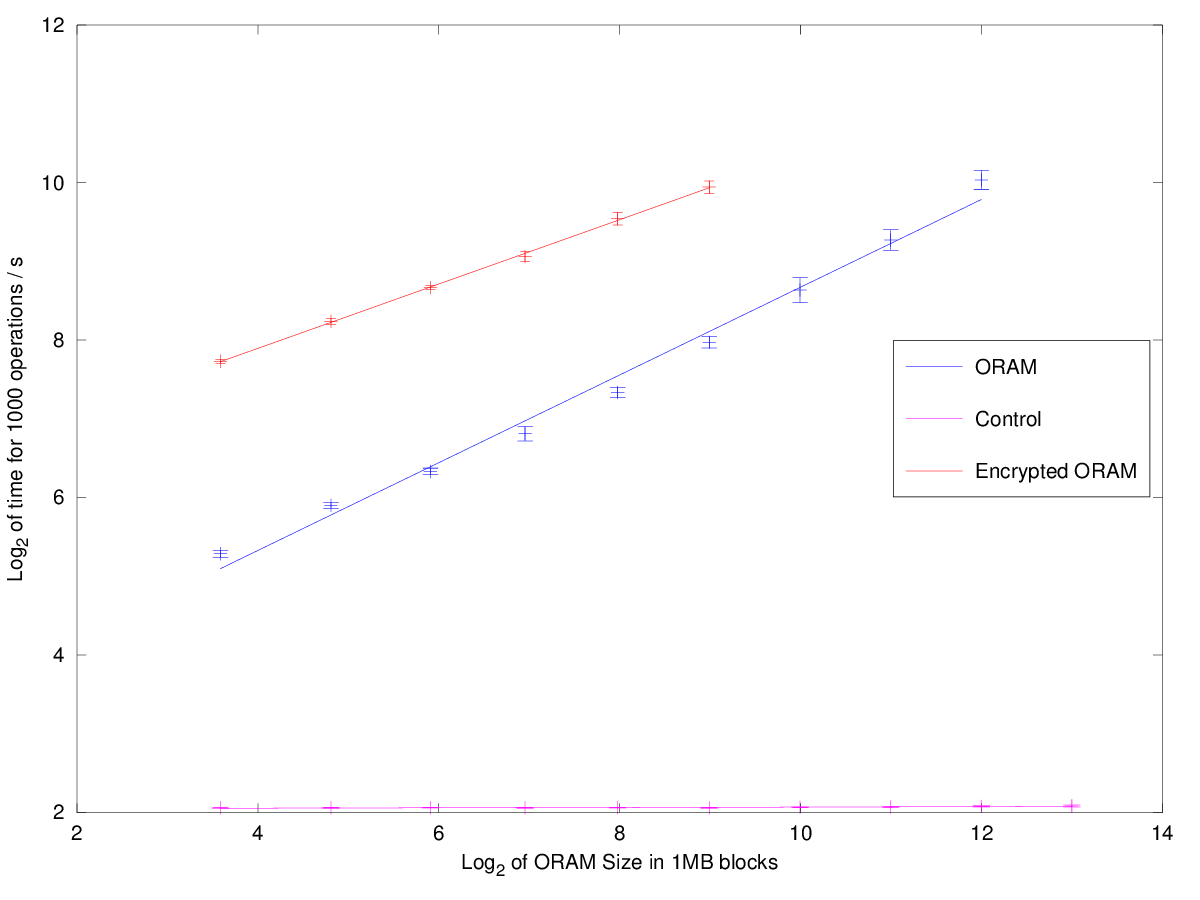
\includegraphics[width=.8\linewidth]{timeResults}
    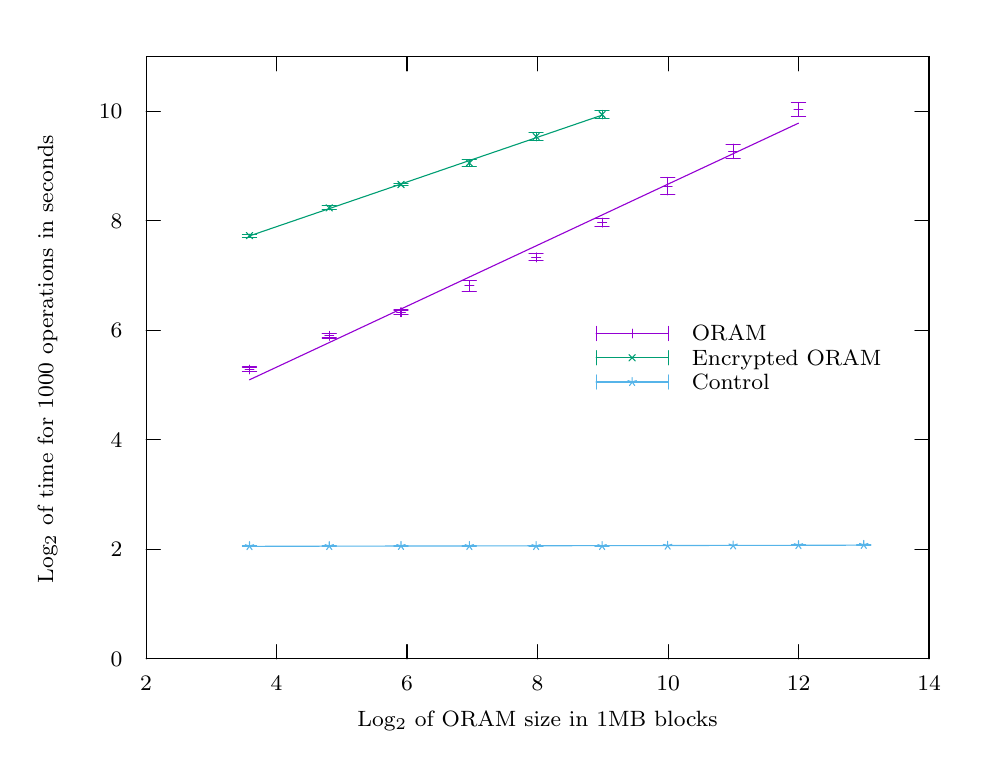
\begin{tikzpicture}[gnuplot]
%% generated with GNUPLOT 5.0p3 (Lua 5.3; terminal rev. 99, script rev. 100)
%% Mon 02 May 2016 10:36:46 BST
\path (0.000,0.000) rectangle (12.000,9.000);
\gpcolor{color=gp lt color border}
\gpsetlinetype{gp lt border}
\gpsetdashtype{gp dt solid}
\gpsetlinewidth{1.00}
\draw[gp path] (1.504,0.985)--(1.684,0.985);
\draw[gp path] (11.447,0.985)--(11.267,0.985);
\node[gp node right] at (1.320,0.985) {\footnotesize 0};
\draw[gp path] (1.504,2.375)--(1.684,2.375);
\draw[gp path] (11.447,2.375)--(11.267,2.375);
\node[gp node right] at (1.320,2.375) {\footnotesize 2};
\draw[gp path] (1.504,3.765)--(1.684,3.765);
\draw[gp path] (11.447,3.765)--(11.267,3.765);
\node[gp node right] at (1.320,3.765) {\footnotesize 4};
\draw[gp path] (1.504,5.156)--(1.684,5.156);
\draw[gp path] (11.447,5.156)--(11.267,5.156);
\node[gp node right] at (1.320,5.156) {\footnotesize 6};
\draw[gp path] (1.504,6.546)--(1.684,6.546);
\draw[gp path] (11.447,6.546)--(11.267,6.546);
\node[gp node right] at (1.320,6.546) {\footnotesize 8};
\draw[gp path] (1.504,7.936)--(1.684,7.936);
\draw[gp path] (11.447,7.936)--(11.267,7.936);
\node[gp node right] at (1.320,7.936) {\footnotesize 10};
\draw[gp path] (1.504,0.985)--(1.504,1.165);
\draw[gp path] (1.504,8.631)--(1.504,8.451);
\node[gp node center] at (1.504,0.677) {\footnotesize 2};
\draw[gp path] (3.161,0.985)--(3.161,1.165);
\draw[gp path] (3.161,8.631)--(3.161,8.451);
\node[gp node center] at (3.161,0.677) {\footnotesize 4};
\draw[gp path] (4.818,0.985)--(4.818,1.165);
\draw[gp path] (4.818,8.631)--(4.818,8.451);
\node[gp node center] at (4.818,0.677) {\footnotesize 6};
\draw[gp path] (6.476,0.985)--(6.476,1.165);
\draw[gp path] (6.476,8.631)--(6.476,8.451);
\node[gp node center] at (6.476,0.677) {\footnotesize 8};
\draw[gp path] (8.133,0.985)--(8.133,1.165);
\draw[gp path] (8.133,8.631)--(8.133,8.451);
\node[gp node center] at (8.133,0.677) {\footnotesize 10};
\draw[gp path] (9.790,0.985)--(9.790,1.165);
\draw[gp path] (9.790,8.631)--(9.790,8.451);
\node[gp node center] at (9.790,0.677) {\footnotesize 12};
\draw[gp path] (11.447,0.985)--(11.447,1.165);
\draw[gp path] (11.447,8.631)--(11.447,8.451);
\node[gp node center] at (11.447,0.677) {\footnotesize 14};
\draw[gp path] (1.504,8.631)--(1.504,0.985)--(11.447,0.985)--(11.447,8.631)--cycle;
\node[gp node center,rotate=-270] at (0.246,4.808) {\footnotesize Log$_2$ of time for 1000 operations in seconds};
\node[gp node center] at (6.475,0.215) {\footnotesize Log$_2$ of ORAM size in 1MB blocks};
\node[gp node left] at (8.319,5.116) {\footnotesize ORAM};
\gpcolor{rgb color={0.580,0.000,0.827}}
\draw[gp path] (7.219,5.116)--(8.135,5.116);
\draw[gp path] (7.219,5.206)--(7.219,5.026);
\draw[gp path] (8.135,5.206)--(8.135,5.026);
\draw[gp path] (2.817,4.629)--(2.817,4.690);
\draw[gp path] (2.727,4.629)--(2.907,4.629);
\draw[gp path] (2.727,4.690)--(2.907,4.690);
\draw[gp path] (3.830,5.059)--(3.830,5.113);
\draw[gp path] (3.740,5.059)--(3.920,5.059);
\draw[gp path] (3.740,5.113)--(3.920,5.113);
\draw[gp path] (4.741,5.356)--(4.741,5.415);
\draw[gp path] (4.651,5.356)--(4.831,5.356);
\draw[gp path] (4.651,5.415)--(4.831,5.415);
\draw[gp path] (5.609,5.655)--(5.609,5.785);
\draw[gp path] (5.519,5.655)--(5.699,5.655);
\draw[gp path] (5.519,5.785)--(5.699,5.785);
\draw[gp path] (6.457,6.039)--(6.457,6.127);
\draw[gp path] (6.367,6.039)--(6.547,6.039);
\draw[gp path] (6.367,6.127)--(6.547,6.127);
\draw[gp path] (7.295,6.476)--(7.295,6.575);
\draw[gp path] (7.205,6.476)--(7.385,6.476);
\draw[gp path] (7.205,6.575)--(7.385,6.575);
\draw[gp path] (8.128,6.876)--(8.128,7.099);
\draw[gp path] (8.038,6.876)--(8.218,6.876);
\draw[gp path] (8.038,7.099)--(8.218,7.099);
\draw[gp path] (8.959,7.338)--(8.959,7.520);
\draw[gp path] (8.869,7.338)--(9.049,7.338);
\draw[gp path] (8.869,7.520)--(9.049,7.520);
\draw[gp path] (9.789,7.876)--(9.789,8.044);
\draw[gp path] (9.699,7.876)--(9.879,7.876);
\draw[gp path] (9.699,8.044)--(9.879,8.044);
\gpsetpointsize{4.00}
\gppoint{gp mark 1}{(2.817,4.659)}
\gppoint{gp mark 1}{(3.830,5.086)}
\gppoint{gp mark 1}{(4.741,5.386)}
\gppoint{gp mark 1}{(5.609,5.720)}
\gppoint{gp mark 1}{(6.457,6.083)}
\gppoint{gp mark 1}{(7.295,6.525)}
\gppoint{gp mark 1}{(8.128,6.987)}
\gppoint{gp mark 1}{(8.959,7.429)}
\gppoint{gp mark 1}{(9.789,7.960)}
\gppoint{gp mark 1}{(7.677,5.116)}
\draw[gp path] (2.817,4.528)--(3.830,5.001)--(4.741,5.427)--(5.609,5.833)--(6.457,6.229)%
  --(7.295,6.621)--(8.128,7.011)--(8.959,7.399)--(9.789,7.787);
\gpcolor{color=gp lt color border}
\node[gp node left] at (8.319,4.808) {\footnotesize Encrypted ORAM};
\gpcolor{rgb color={0.000,0.620,0.451}}
\draw[gp path] (7.219,4.808)--(8.135,4.808);
\draw[gp path] (7.219,4.898)--(7.219,4.718);
\draw[gp path] (8.135,4.898)--(8.135,4.718);
\draw[gp path] (2.817,6.340)--(2.817,6.377);
\draw[gp path] (2.727,6.340)--(2.907,6.340);
\draw[gp path] (2.727,6.377)--(2.907,6.377);
\draw[gp path] (3.830,6.686)--(3.830,6.738);
\draw[gp path] (3.740,6.686)--(3.920,6.686);
\draw[gp path] (3.740,6.738)--(3.920,6.738);
\draw[gp path] (4.741,6.993)--(4.741,7.024);
\draw[gp path] (4.651,6.993)--(4.831,6.993);
\draw[gp path] (4.651,7.024)--(4.831,7.024);
\draw[gp path] (5.609,7.238)--(5.609,7.326);
\draw[gp path] (5.519,7.238)--(5.699,7.238);
\draw[gp path] (5.519,7.326)--(5.699,7.326);
\draw[gp path] (6.457,7.563)--(6.457,7.671);
\draw[gp path] (6.367,7.563)--(6.547,7.563);
\draw[gp path] (6.367,7.671)--(6.547,7.671);
\draw[gp path] (7.295,7.842)--(7.295,7.950);
\draw[gp path] (7.205,7.842)--(7.385,7.842);
\draw[gp path] (7.205,7.950)--(7.385,7.950);
\gppoint{gp mark 2}{(2.817,6.358)}
\gppoint{gp mark 2}{(3.830,6.712)}
\gppoint{gp mark 2}{(4.741,7.008)}
\gppoint{gp mark 2}{(5.609,7.282)}
\gppoint{gp mark 2}{(6.457,7.617)}
\gppoint{gp mark 2}{(7.295,7.896)}
\gppoint{gp mark 2}{(7.677,4.808)}
\draw[gp path] (2.817,6.355)--(3.830,6.702)--(4.741,7.014)--(5.609,7.312)--(6.457,7.602)%
  --(7.295,7.889);
\gpcolor{color=gp lt color border}
\node[gp node left] at (8.319,4.500) {\footnotesize Control};
\gpcolor{rgb color={0.337,0.706,0.914}}
\draw[gp path] (7.219,4.500)--(8.135,4.500);
\draw[gp path] (7.219,4.590)--(7.219,4.410);
\draw[gp path] (8.135,4.590)--(8.135,4.410);
\draw[gp path] (2.817,2.413)--(2.817,2.419);
\draw[gp path] (2.727,2.413)--(2.907,2.413);
\draw[gp path] (2.727,2.419)--(2.907,2.419);
\draw[gp path] (3.830,2.414)--(3.830,2.419);
\draw[gp path] (3.740,2.414)--(3.920,2.414);
\draw[gp path] (3.740,2.419)--(3.920,2.419);
\draw[gp path] (4.741,2.415)--(4.741,2.420);
\draw[gp path] (4.651,2.415)--(4.831,2.415);
\draw[gp path] (4.651,2.420)--(4.831,2.420);
\draw[gp path] (5.609,2.414)--(5.609,2.420);
\draw[gp path] (5.519,2.414)--(5.699,2.414);
\draw[gp path] (5.519,2.420)--(5.699,2.420);
\draw[gp path] (6.457,2.416)--(6.457,2.419);
\draw[gp path] (6.367,2.416)--(6.547,2.416);
\draw[gp path] (6.367,2.419)--(6.547,2.419);
\draw[gp path] (7.295,2.413)--(7.295,2.420);
\draw[gp path] (7.205,2.413)--(7.385,2.413);
\draw[gp path] (7.205,2.420)--(7.385,2.420);
\draw[gp path] (8.128,2.418)--(8.128,2.424);
\draw[gp path] (8.038,2.418)--(8.218,2.418);
\draw[gp path] (8.038,2.424)--(8.218,2.424);
\draw[gp path] (8.959,2.419)--(8.959,2.428);
\draw[gp path] (8.869,2.419)--(9.049,2.419);
\draw[gp path] (8.869,2.428)--(9.049,2.428);
\draw[gp path] (9.789,2.425)--(9.789,2.434);
\draw[gp path] (9.699,2.425)--(9.879,2.425);
\draw[gp path] (9.699,2.434)--(9.879,2.434);
\draw[gp path] (10.618,2.423)--(10.618,2.440);
\draw[gp path] (10.528,2.423)--(10.708,2.423);
\draw[gp path] (10.528,2.440)--(10.708,2.440);
\gppoint{gp mark 3}{(2.817,2.416)}
\gppoint{gp mark 3}{(3.830,2.417)}
\gppoint{gp mark 3}{(4.741,2.418)}
\gppoint{gp mark 3}{(5.609,2.417)}
\gppoint{gp mark 3}{(6.457,2.417)}
\gppoint{gp mark 3}{(7.295,2.417)}
\gppoint{gp mark 3}{(8.128,2.421)}
\gppoint{gp mark 3}{(8.959,2.424)}
\gppoint{gp mark 3}{(9.789,2.429)}
\gppoint{gp mark 3}{(10.618,2.432)}
\gppoint{gp mark 3}{(7.677,4.500)}
\draw[gp path] (2.817,2.413)--(3.830,2.415)--(4.741,2.417)--(5.609,2.418)--(6.457,2.420)%
  --(7.295,2.422)--(8.128,2.423)--(8.959,2.425)--(9.789,2.426)--(10.618,2.428);
\gpcolor{color=gp lt color border}
\draw[gp path] (1.504,8.631)--(1.504,0.985)--(11.447,0.985)--(11.447,8.631)--cycle;
%% coordinates of the plot area
\gpdefrectangularnode{gp plot 1}{\pgfpoint{1.504cm}{0.985cm}}{\pgfpoint{11.447cm}{8.631cm}}
\end{tikzpicture}

    \caption{The relationship between size of an ORAM in blocks and the time taken for 1000 operations, plotted for ORAM, encrypted ORAM, and a control block device with no ORAM. We take logs of both axes, because block size was increased in powers of two and we expect a log relationship.}
    \label{fig:timeResults}
\end{figure}

%The initialisation phase allowed the stash size to reach a steady state, which resulted in a constant overhead of $x$ blocks, compared with $y$ predicted in \citet{stefanov2013path} for a security parameter, $\lambda = z$. This shows something...

%In these first experiments, we used stateless, non-recursive ORAM, which means that the entire of the position map was being flushed to disk on every access. We now compare the time taken for stateless, recursive ORAM, to see what effect the additional recursive calls have compared to the reduction in the size of the client side state. We can see from \cref{fig:recursiveTimePlot} that overall this was good/bad to some degree.

Although it has not been discussed here, bandwidth is another important measure when examining the performance of ORAM, especially when it is being used in the cloud. With more time, a detailed study of the bandwidth used with and without recursion would have been carried out, which would have given insight into the trade-off that recursion presents us with.

\section{Statistical Analysis}
\label{sec:statisticalAnalysis}

To demonstrate the effectiveness of ORAM, it must be shown that the access pattern observed by the block device is statistically random. There is structure to this randomness, because on each access a whole path is read and written. For a tree of height $L$, $L+1$ accesses are made, each to a subrange that corresponds to a level of the tree. However, the actual path that is written should be random. Thus, a test for randomness should be performed on a sequence of path indices.

I used two techniques: autocorrelation plotting and runs testing.

Autocorrelation plotting plots the correlation of a sequence with itself at various time lags \cite{nistautocorr}. For a random sequence, the noise cancels itself out, resulting in a plot of values very close to zero. The exception is lag 0, where the correlation will be exactly the power of the signal. I plotted this for two access patterns: one of length 200, for which the results would be easily visible; and one of length 5,000, to show longer term effects. For both of these patterns, the underlying access pattern, which would be seen without ORAM, was simply a succession of reads and writes to the same location. These plots are shown in \cref{fig:shortAutocorr} and \cref{fig:longAutocorr} respectively.

\begin{figure}
    \centering
    \begin{subfigure}{\textwidth}
        \centering
        %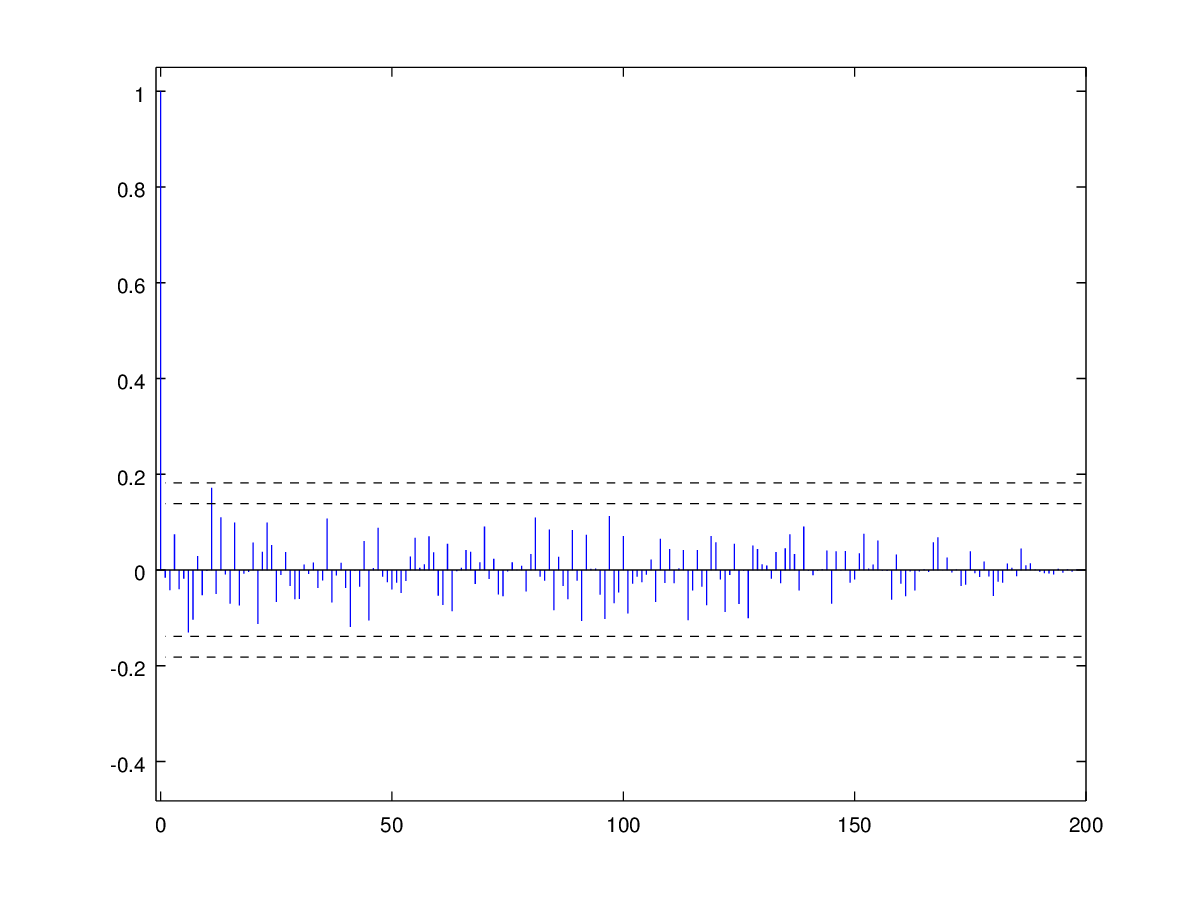
\includegraphics[width=\linewidth]{shortAutocorr}
        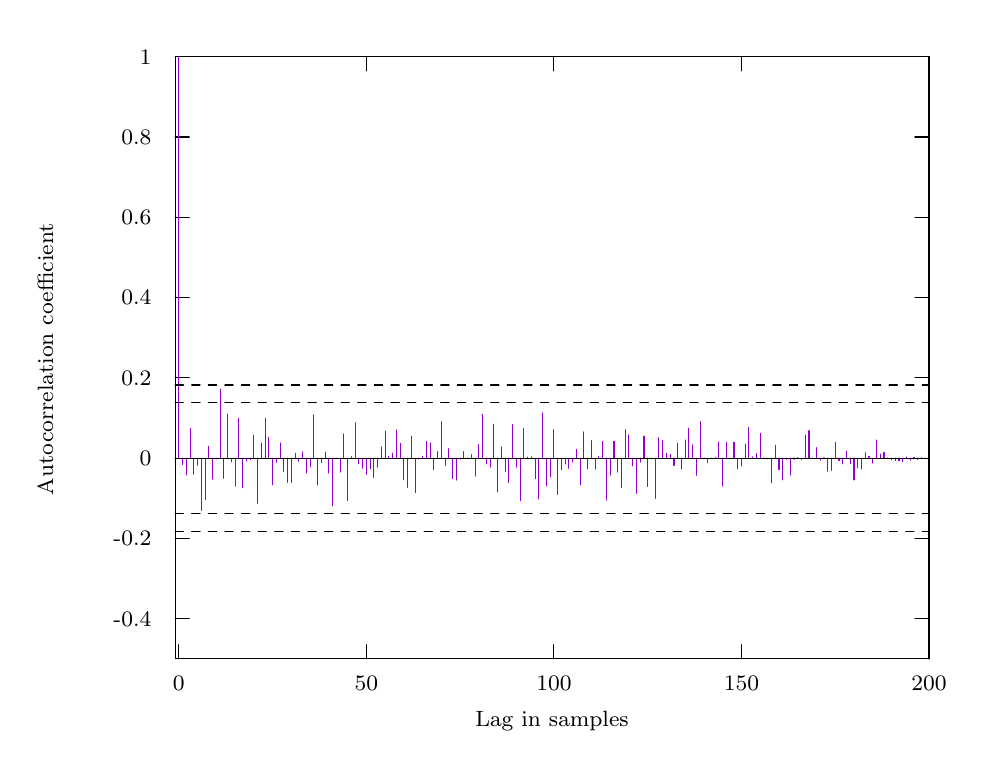
\begin{tikzpicture}[gnuplot]
%% generated with GNUPLOT 5.0p3 (Lua 5.3; terminal rev. 99, script rev. 100)
%% Mon 02 May 2016 08:41:38 BST
\path (0.000,0.000) rectangle (12.000,9.000);
\gpcolor{color=gp lt color border}
\gpsetlinetype{gp lt border}
\gpsetdashtype{gp dt solid}
\gpsetlinewidth{1.00}
\draw[gp path] (1.872,1.495)--(2.052,1.495);
\draw[gp path] (11.447,1.495)--(11.267,1.495);
\node[gp node right] at (1.688,1.495) {\footnotesize -0.4};
\draw[gp path] (1.872,2.514)--(2.052,2.514);
\draw[gp path] (11.447,2.514)--(11.267,2.514);
\node[gp node right] at (1.688,2.514) {\footnotesize -0.2};
\draw[gp path] (1.872,3.534)--(2.052,3.534);
\draw[gp path] (11.447,3.534)--(11.267,3.534);
\node[gp node right] at (1.688,3.534) {\footnotesize 0};
\draw[gp path] (1.872,4.553)--(2.052,4.553);
\draw[gp path] (11.447,4.553)--(11.267,4.553);
\node[gp node right] at (1.688,4.553) {\footnotesize 0.2};
\draw[gp path] (1.872,5.573)--(2.052,5.573);
\draw[gp path] (11.447,5.573)--(11.267,5.573);
\node[gp node right] at (1.688,5.573) {\footnotesize 0.4};
\draw[gp path] (1.872,6.592)--(2.052,6.592);
\draw[gp path] (11.447,6.592)--(11.267,6.592);
\node[gp node right] at (1.688,6.592) {\footnotesize 0.6};
\draw[gp path] (1.872,7.612)--(2.052,7.612);
\draw[gp path] (11.447,7.612)--(11.267,7.612);
\node[gp node right] at (1.688,7.612) {\footnotesize 0.8};
\draw[gp path] (1.872,8.631)--(2.052,8.631);
\draw[gp path] (11.447,8.631)--(11.267,8.631);
\node[gp node right] at (1.688,8.631) {\footnotesize 1};
\draw[gp path] (1.920,0.985)--(1.920,1.165);
\draw[gp path] (1.920,8.631)--(1.920,8.451);
\node[gp node center] at (1.920,0.677) {\footnotesize 0};
\draw[gp path] (4.301,0.985)--(4.301,1.165);
\draw[gp path] (4.301,8.631)--(4.301,8.451);
\node[gp node center] at (4.301,0.677) {\footnotesize 50};
\draw[gp path] (6.683,0.985)--(6.683,1.165);
\draw[gp path] (6.683,8.631)--(6.683,8.451);
\node[gp node center] at (6.683,0.677) {\footnotesize 100};
\draw[gp path] (9.065,0.985)--(9.065,1.165);
\draw[gp path] (9.065,8.631)--(9.065,8.451);
\node[gp node center] at (9.065,0.677) {\footnotesize 150};
\draw[gp path] (11.447,0.985)--(11.447,1.165);
\draw[gp path] (11.447,8.631)--(11.447,8.451);
\node[gp node center] at (11.447,0.677) {\footnotesize 200};
\draw[gp path] (1.872,8.631)--(1.872,0.985)--(11.447,0.985)--(11.447,8.631)--cycle;
\node[gp node center,rotate=-270] at (0.246,4.808) {\footnotesize Autocorrelation coefficient};
\node[gp node center] at (6.659,0.215) {\footnotesize Lag in samples};
\gpcolor{rgb color={0.580,0.000,0.827}}
\draw[gp path] (1.920,3.534)--(1.920,8.631);
\draw[gp path] (1.967,3.534)--(1.967,3.452);
\draw[gp path] (2.015,3.534)--(2.015,3.320);
\draw[gp path] (2.063,3.534)--(2.063,3.912);
\draw[gp path] (2.110,3.534)--(2.110,3.330);
\draw[gp path] (2.158,3.534)--(2.158,3.443);
\draw[gp path] (2.205,3.534)--(2.205,2.870);
\draw[gp path] (2.253,3.534)--(2.253,3.007);
\draw[gp path] (2.301,3.534)--(2.301,3.682);
\draw[gp path] (2.348,3.534)--(2.348,3.267);
\draw[gp path] (2.396,3.534)--(2.396,3.524);
\draw[gp path] (2.444,3.534)--(2.444,4.408);
\draw[gp path] (2.491,3.534)--(2.491,3.278);
\draw[gp path] (2.539,3.534)--(2.539,4.093);
\draw[gp path] (2.587,3.534)--(2.587,3.487);
\draw[gp path] (2.634,3.534)--(2.634,3.177);
\draw[gp path] (2.682,3.534)--(2.682,4.037);
\draw[gp path] (2.729,3.534)--(2.729,3.158);
\draw[gp path] (2.777,3.534)--(2.777,3.495);
\draw[gp path] (2.825,3.534)--(2.825,3.514);
\draw[gp path] (2.872,3.534)--(2.872,3.825);
\draw[gp path] (2.920,3.534)--(2.920,2.960);
\draw[gp path] (2.968,3.534)--(2.968,3.727);
\draw[gp path] (3.015,3.534)--(3.015,4.039);
\draw[gp path] (3.063,3.534)--(3.063,3.799);
\draw[gp path] (3.111,3.534)--(3.111,3.195);
\draw[gp path] (3.158,3.534)--(3.158,3.483);
\draw[gp path] (3.206,3.534)--(3.206,3.725);
\draw[gp path] (3.253,3.534)--(3.253,3.365);
\draw[gp path] (3.301,3.534)--(3.301,3.225);
\draw[gp path] (3.349,3.534)--(3.349,3.227);
\draw[gp path] (3.396,3.534)--(3.396,3.592);
\draw[gp path] (3.444,3.534)--(3.444,3.494);
\draw[gp path] (3.492,3.534)--(3.492,3.613);
\draw[gp path] (3.539,3.534)--(3.539,3.345);
\draw[gp path] (3.587,3.534)--(3.587,3.423);
\draw[gp path] (3.635,3.534)--(3.635,4.081);
\draw[gp path] (3.682,3.534)--(3.682,3.190);
\draw[gp path] (3.730,3.534)--(3.730,3.477);
\draw[gp path] (3.777,3.534)--(3.777,3.609);
\draw[gp path] (3.825,3.534)--(3.825,3.344);
\draw[gp path] (3.873,3.534)--(3.873,2.928);
\draw[gp path] (3.920,3.534)--(3.920,3.526);
\draw[gp path] (3.968,3.534)--(3.968,3.357);
\draw[gp path] (4.016,3.534)--(4.016,3.841);
\draw[gp path] (4.063,3.534)--(4.063,2.997);
\draw[gp path] (4.111,3.534)--(4.111,3.553);
\draw[gp path] (4.159,3.534)--(4.159,3.982);
\draw[gp path] (4.206,3.534)--(4.206,3.465);
\draw[gp path] (4.254,3.534)--(4.254,3.405);
\draw[gp path] (4.301,3.534)--(4.301,3.327);
\draw[gp path] (4.349,3.534)--(4.349,3.400);
\draw[gp path] (4.397,3.534)--(4.397,3.290);
\draw[gp path] (4.444,3.534)--(4.444,3.418);
\draw[gp path] (4.492,3.534)--(4.492,3.676);
\draw[gp path] (4.540,3.534)--(4.540,3.875);
\draw[gp path] (4.587,3.534)--(4.587,3.556);
\draw[gp path] (4.635,3.534)--(4.635,3.592);
\draw[gp path] (4.683,3.534)--(4.683,3.891);
\draw[gp path] (4.730,3.534)--(4.730,3.721);
\draw[gp path] (4.778,3.534)--(4.778,3.262);
\draw[gp path] (4.825,3.534)--(4.825,3.162);
\draw[gp path] (4.873,3.534)--(4.873,3.812);
\draw[gp path] (4.921,3.534)--(4.921,3.096);
\draw[gp path] (4.968,3.534)--(4.968,3.521);
\draw[gp path] (5.016,3.534)--(5.016,3.556);
\draw[gp path] (5.064,3.534)--(5.064,3.746);
\draw[gp path] (5.111,3.534)--(5.111,3.727);
\draw[gp path] (5.159,3.534)--(5.159,3.387);
\draw[gp path] (5.207,3.534)--(5.207,3.616);
\draw[gp path] (5.254,3.534)--(5.254,3.995);
\draw[gp path] (5.302,3.534)--(5.302,3.438);
\draw[gp path] (5.349,3.534)--(5.349,3.652);
\draw[gp path] (5.397,3.534)--(5.397,3.274);
\draw[gp path] (5.445,3.534)--(5.445,3.255);
\draw[gp path] (5.492,3.534)--(5.492,3.520);
\draw[gp path] (5.540,3.534)--(5.540,3.616);
\draw[gp path] (5.588,3.534)--(5.588,3.536);
\draw[gp path] (5.635,3.534)--(5.635,3.577);
\draw[gp path] (5.683,3.534)--(5.683,3.305);
\draw[gp path] (5.731,3.534)--(5.731,3.703);
\draw[gp path] (5.778,3.534)--(5.778,4.092);
\draw[gp path] (5.826,3.534)--(5.826,3.462);
\draw[gp path] (5.873,3.534)--(5.873,3.420);
\draw[gp path] (5.921,3.534)--(5.921,3.963);
\draw[gp path] (5.969,3.534)--(5.969,3.105);
\draw[gp path] (6.016,3.534)--(6.016,3.674);
\draw[gp path] (6.064,3.534)--(6.064,3.364);
\draw[gp path] (6.112,3.534)--(6.112,3.224);
\draw[gp path] (6.159,3.534)--(6.159,3.957);
\draw[gp path] (6.207,3.534)--(6.207,3.420);
\draw[gp path] (6.255,3.534)--(6.255,2.993);
\draw[gp path] (6.302,3.534)--(6.302,3.908);
\draw[gp path] (6.350,3.534)--(6.350,3.545);
\draw[gp path] (6.397,3.534)--(6.397,3.549);
\draw[gp path] (6.445,3.534)--(6.445,3.272);
\draw[gp path] (6.493,3.534)--(6.493,3.015);
\draw[gp path] (6.540,3.534)--(6.540,4.108);
\draw[gp path] (6.588,3.534)--(6.588,3.182);
\draw[gp path] (6.636,3.534)--(6.636,3.295);
\draw[gp path] (6.683,3.534)--(6.683,3.895);
\draw[gp path] (6.731,3.534)--(6.731,3.072);
\draw[gp path] (6.779,3.534)--(6.779,3.388);
\draw[gp path] (6.826,3.534)--(6.826,3.462);
\draw[gp path] (6.874,3.534)--(6.874,3.405);
\draw[gp path] (6.922,3.534)--(6.922,3.485);
\draw[gp path] (6.969,3.534)--(6.969,3.644);
\draw[gp path] (7.017,3.534)--(7.017,3.195);
\draw[gp path] (7.064,3.534)--(7.064,3.866);
\draw[gp path] (7.112,3.534)--(7.112,3.397);
\draw[gp path] (7.160,3.534)--(7.160,3.756);
\draw[gp path] (7.207,3.534)--(7.207,3.394);
\draw[gp path] (7.255,3.534)--(7.255,3.551);
\draw[gp path] (7.303,3.534)--(7.303,3.745);
\draw[gp path] (7.350,3.534)--(7.350,3.001);
\draw[gp path] (7.398,3.534)--(7.398,3.317);
\draw[gp path] (7.446,3.534)--(7.446,3.746);
\draw[gp path] (7.493,3.534)--(7.493,3.357);
\draw[gp path] (7.541,3.534)--(7.541,3.160);
\draw[gp path] (7.588,3.534)--(7.588,3.895);
\draw[gp path] (7.636,3.534)--(7.636,3.828);
\draw[gp path] (7.684,3.534)--(7.684,3.435);
\draw[gp path] (7.731,3.534)--(7.731,3.087);
\draw[gp path] (7.779,3.534)--(7.779,3.483);
\draw[gp path] (7.827,3.534)--(7.827,3.812);
\draw[gp path] (7.874,3.534)--(7.874,3.174);
\draw[gp path] (7.922,3.534)--(7.922,3.527);
\draw[gp path] (7.970,3.534)--(7.970,3.021);
\draw[gp path] (8.017,3.534)--(8.017,3.794);
\draw[gp path] (8.065,3.534)--(8.065,3.756);
\draw[gp path] (8.112,3.534)--(8.112,3.594);
\draw[gp path] (8.160,3.534)--(8.160,3.581);
\draw[gp path] (8.208,3.534)--(8.208,3.441);
\draw[gp path] (8.255,3.534)--(8.255,3.723);
\draw[gp path] (8.303,3.534)--(8.303,3.394);
\draw[gp path] (8.351,3.534)--(8.351,3.763);
\draw[gp path] (8.398,3.534)--(8.398,3.914);
\draw[gp path] (8.446,3.534)--(8.446,3.702);
\draw[gp path] (8.494,3.534)--(8.494,3.316);
\draw[gp path] (8.541,3.534)--(8.541,3.996);
\draw[gp path] (8.589,3.534)--(8.589,3.526);
\draw[gp path] (8.636,3.534)--(8.636,3.478);
\draw[gp path] (8.684,3.534)--(8.684,3.528);
\draw[gp path] (8.732,3.534)--(8.732,3.539);
\draw[gp path] (8.779,3.534)--(8.779,3.740);
\draw[gp path] (8.827,3.534)--(8.827,3.177);
\draw[gp path] (8.875,3.534)--(8.875,3.732);
\draw[gp path] (8.922,3.534)--(8.922,3.529);
\draw[gp path] (8.970,3.534)--(8.970,3.735);
\draw[gp path] (9.018,3.534)--(9.018,3.399);
\draw[gp path] (9.065,3.534)--(9.065,3.435);
\draw[gp path] (9.113,3.534)--(9.113,3.710);
\draw[gp path] (9.160,3.534)--(9.160,3.919);
\draw[gp path] (9.208,3.534)--(9.208,3.548);
\draw[gp path] (9.256,3.534)--(9.256,3.591);
\draw[gp path] (9.303,3.534)--(9.303,3.846);
\draw[gp path] (9.351,3.534)--(9.351,3.526);
\draw[gp path] (9.399,3.534)--(9.399,3.524);
\draw[gp path] (9.446,3.534)--(9.446,3.218);
\draw[gp path] (9.494,3.534)--(9.494,3.696);
\draw[gp path] (9.542,3.534)--(9.542,3.388);
\draw[gp path] (9.589,3.534)--(9.589,3.257);
\draw[gp path] (9.637,3.534)--(9.637,3.518);
\draw[gp path] (9.684,3.534)--(9.684,3.317);
\draw[gp path] (9.732,3.534)--(9.732,3.520);
\draw[gp path] (9.780,3.534)--(9.780,3.540);
\draw[gp path] (9.827,3.534)--(9.827,3.513);
\draw[gp path] (9.875,3.534)--(9.875,3.828);
\draw[gp path] (9.923,3.534)--(9.923,3.882);
\draw[gp path] (9.970,3.534)--(9.970,3.532);
\draw[gp path] (10.018,3.534)--(10.018,3.666);
\draw[gp path] (10.066,3.534)--(10.066,3.508);
\draw[gp path] (10.113,3.534)--(10.113,3.537);
\draw[gp path] (10.161,3.534)--(10.161,3.364);
\draw[gp path] (10.208,3.534)--(10.208,3.377);
\draw[gp path] (10.256,3.534)--(10.256,3.732);
\draw[gp path] (10.304,3.534)--(10.304,3.502);
\draw[gp path] (10.351,3.534)--(10.351,3.462);
\draw[gp path] (10.399,3.534)--(10.399,3.622);
\draw[gp path] (10.447,3.534)--(10.447,3.465);
\draw[gp path] (10.494,3.534)--(10.494,3.257);
\draw[gp path] (10.542,3.534)--(10.542,3.409);
\draw[gp path] (10.590,3.534)--(10.590,3.398);
\draw[gp path] (10.637,3.534)--(10.637,3.601);
\draw[gp path] (10.685,3.534)--(10.685,3.555);
\draw[gp path] (10.732,3.534)--(10.732,3.469);
\draw[gp path] (10.780,3.534)--(10.780,3.763);
\draw[gp path] (10.828,3.534)--(10.828,3.583);
\draw[gp path] (10.875,3.534)--(10.875,3.605);
\draw[gp path] (10.923,3.534)--(10.923,3.537);
\draw[gp path] (10.971,3.534)--(10.971,3.516);
\draw[gp path] (11.018,3.534)--(11.018,3.501);
\draw[gp path] (11.066,3.534)--(11.066,3.499);
\draw[gp path] (11.114,3.534)--(11.114,3.488);
\draw[gp path] (11.161,3.534)--(11.161,3.547);
\draw[gp path] (11.209,3.534)--(11.209,3.507);
\draw[gp path] (11.256,3.534)--(11.256,3.542);
\draw[gp path] (11.304,3.534)--(11.304,3.517);
\draw[gp path] (11.352,3.534)--(11.352,3.539);
\draw[gp path] (11.399,3.534)--(11.399,3.527);
\gpcolor{rgb color={0.000,0.000,0.000}}
\gpsetdashtype{gp dt 2}
\draw[gp path] (1.872,4.240)--(1.969,4.240)--(2.065,4.240)--(2.162,4.240)--(2.259,4.240)%
  --(2.356,4.240)--(2.452,4.240)--(2.549,4.240)--(2.646,4.240)--(2.742,4.240)--(2.839,4.240)%
  --(2.936,4.240)--(3.033,4.240)--(3.129,4.240)--(3.226,4.240)--(3.323,4.240)--(3.419,4.240)%
  --(3.516,4.240)--(3.613,4.240)--(3.710,4.240)--(3.806,4.240)--(3.903,4.240)--(4.000,4.240)%
  --(4.096,4.240)--(4.193,4.240)--(4.290,4.240)--(4.387,4.240)--(4.483,4.240)--(4.580,4.240)%
  --(4.677,4.240)--(4.774,4.240)--(4.870,4.240)--(4.967,4.240)--(5.064,4.240)--(5.160,4.240)%
  --(5.257,4.240)--(5.354,4.240)--(5.451,4.240)--(5.547,4.240)--(5.644,4.240)--(5.741,4.240)%
  --(5.837,4.240)--(5.934,4.240)--(6.031,4.240)--(6.128,4.240)--(6.224,4.240)--(6.321,4.240)%
  --(6.418,4.240)--(6.514,4.240)--(6.611,4.240)--(6.708,4.240)--(6.805,4.240)--(6.901,4.240)%
  --(6.998,4.240)--(7.095,4.240)--(7.191,4.240)--(7.288,4.240)--(7.385,4.240)--(7.482,4.240)%
  --(7.578,4.240)--(7.675,4.240)--(7.772,4.240)--(7.868,4.240)--(7.965,4.240)--(8.062,4.240)%
  --(8.159,4.240)--(8.255,4.240)--(8.352,4.240)--(8.449,4.240)--(8.545,4.240)--(8.642,4.240)%
  --(8.739,4.240)--(8.836,4.240)--(8.932,4.240)--(9.029,4.240)--(9.126,4.240)--(9.223,4.240)%
  --(9.319,4.240)--(9.416,4.240)--(9.513,4.240)--(9.609,4.240)--(9.706,4.240)--(9.803,4.240)%
  --(9.900,4.240)--(9.996,4.240)--(10.093,4.240)--(10.190,4.240)--(10.286,4.240)--(10.383,4.240)%
  --(10.480,4.240)--(10.577,4.240)--(10.673,4.240)--(10.770,4.240)--(10.867,4.240)--(10.963,4.240)%
  --(11.060,4.240)--(11.157,4.240)--(11.254,4.240)--(11.350,4.240)--(11.447,4.240);
\draw[gp path] (1.872,2.827)--(1.969,2.827)--(2.065,2.827)--(2.162,2.827)--(2.259,2.827)%
  --(2.356,2.827)--(2.452,2.827)--(2.549,2.827)--(2.646,2.827)--(2.742,2.827)--(2.839,2.827)%
  --(2.936,2.827)--(3.033,2.827)--(3.129,2.827)--(3.226,2.827)--(3.323,2.827)--(3.419,2.827)%
  --(3.516,2.827)--(3.613,2.827)--(3.710,2.827)--(3.806,2.827)--(3.903,2.827)--(4.000,2.827)%
  --(4.096,2.827)--(4.193,2.827)--(4.290,2.827)--(4.387,2.827)--(4.483,2.827)--(4.580,2.827)%
  --(4.677,2.827)--(4.774,2.827)--(4.870,2.827)--(4.967,2.827)--(5.064,2.827)--(5.160,2.827)%
  --(5.257,2.827)--(5.354,2.827)--(5.451,2.827)--(5.547,2.827)--(5.644,2.827)--(5.741,2.827)%
  --(5.837,2.827)--(5.934,2.827)--(6.031,2.827)--(6.128,2.827)--(6.224,2.827)--(6.321,2.827)%
  --(6.418,2.827)--(6.514,2.827)--(6.611,2.827)--(6.708,2.827)--(6.805,2.827)--(6.901,2.827)%
  --(6.998,2.827)--(7.095,2.827)--(7.191,2.827)--(7.288,2.827)--(7.385,2.827)--(7.482,2.827)%
  --(7.578,2.827)--(7.675,2.827)--(7.772,2.827)--(7.868,2.827)--(7.965,2.827)--(8.062,2.827)%
  --(8.159,2.827)--(8.255,2.827)--(8.352,2.827)--(8.449,2.827)--(8.545,2.827)--(8.642,2.827)%
  --(8.739,2.827)--(8.836,2.827)--(8.932,2.827)--(9.029,2.827)--(9.126,2.827)--(9.223,2.827)%
  --(9.319,2.827)--(9.416,2.827)--(9.513,2.827)--(9.609,2.827)--(9.706,2.827)--(9.803,2.827)%
  --(9.900,2.827)--(9.996,2.827)--(10.093,2.827)--(10.190,2.827)--(10.286,2.827)--(10.383,2.827)%
  --(10.480,2.827)--(10.577,2.827)--(10.673,2.827)--(10.770,2.827)--(10.867,2.827)--(10.963,2.827)%
  --(11.060,2.827)--(11.157,2.827)--(11.254,2.827)--(11.350,2.827)--(11.447,2.827);
\draw[gp path] (1.872,4.462)--(1.969,4.462)--(2.065,4.462)--(2.162,4.462)--(2.259,4.462)%
  --(2.356,4.462)--(2.452,4.462)--(2.549,4.462)--(2.646,4.462)--(2.742,4.462)--(2.839,4.462)%
  --(2.936,4.462)--(3.033,4.462)--(3.129,4.462)--(3.226,4.462)--(3.323,4.462)--(3.419,4.462)%
  --(3.516,4.462)--(3.613,4.462)--(3.710,4.462)--(3.806,4.462)--(3.903,4.462)--(4.000,4.462)%
  --(4.096,4.462)--(4.193,4.462)--(4.290,4.462)--(4.387,4.462)--(4.483,4.462)--(4.580,4.462)%
  --(4.677,4.462)--(4.774,4.462)--(4.870,4.462)--(4.967,4.462)--(5.064,4.462)--(5.160,4.462)%
  --(5.257,4.462)--(5.354,4.462)--(5.451,4.462)--(5.547,4.462)--(5.644,4.462)--(5.741,4.462)%
  --(5.837,4.462)--(5.934,4.462)--(6.031,4.462)--(6.128,4.462)--(6.224,4.462)--(6.321,4.462)%
  --(6.418,4.462)--(6.514,4.462)--(6.611,4.462)--(6.708,4.462)--(6.805,4.462)--(6.901,4.462)%
  --(6.998,4.462)--(7.095,4.462)--(7.191,4.462)--(7.288,4.462)--(7.385,4.462)--(7.482,4.462)%
  --(7.578,4.462)--(7.675,4.462)--(7.772,4.462)--(7.868,4.462)--(7.965,4.462)--(8.062,4.462)%
  --(8.159,4.462)--(8.255,4.462)--(8.352,4.462)--(8.449,4.462)--(8.545,4.462)--(8.642,4.462)%
  --(8.739,4.462)--(8.836,4.462)--(8.932,4.462)--(9.029,4.462)--(9.126,4.462)--(9.223,4.462)%
  --(9.319,4.462)--(9.416,4.462)--(9.513,4.462)--(9.609,4.462)--(9.706,4.462)--(9.803,4.462)%
  --(9.900,4.462)--(9.996,4.462)--(10.093,4.462)--(10.190,4.462)--(10.286,4.462)--(10.383,4.462)%
  --(10.480,4.462)--(10.577,4.462)--(10.673,4.462)--(10.770,4.462)--(10.867,4.462)--(10.963,4.462)%
  --(11.060,4.462)--(11.157,4.462)--(11.254,4.462)--(11.350,4.462)--(11.447,4.462);
\draw[gp path] (1.872,2.605)--(1.969,2.605)--(2.065,2.605)--(2.162,2.605)--(2.259,2.605)%
  --(2.356,2.605)--(2.452,2.605)--(2.549,2.605)--(2.646,2.605)--(2.742,2.605)--(2.839,2.605)%
  --(2.936,2.605)--(3.033,2.605)--(3.129,2.605)--(3.226,2.605)--(3.323,2.605)--(3.419,2.605)%
  --(3.516,2.605)--(3.613,2.605)--(3.710,2.605)--(3.806,2.605)--(3.903,2.605)--(4.000,2.605)%
  --(4.096,2.605)--(4.193,2.605)--(4.290,2.605)--(4.387,2.605)--(4.483,2.605)--(4.580,2.605)%
  --(4.677,2.605)--(4.774,2.605)--(4.870,2.605)--(4.967,2.605)--(5.064,2.605)--(5.160,2.605)%
  --(5.257,2.605)--(5.354,2.605)--(5.451,2.605)--(5.547,2.605)--(5.644,2.605)--(5.741,2.605)%
  --(5.837,2.605)--(5.934,2.605)--(6.031,2.605)--(6.128,2.605)--(6.224,2.605)--(6.321,2.605)%
  --(6.418,2.605)--(6.514,2.605)--(6.611,2.605)--(6.708,2.605)--(6.805,2.605)--(6.901,2.605)%
  --(6.998,2.605)--(7.095,2.605)--(7.191,2.605)--(7.288,2.605)--(7.385,2.605)--(7.482,2.605)%
  --(7.578,2.605)--(7.675,2.605)--(7.772,2.605)--(7.868,2.605)--(7.965,2.605)--(8.062,2.605)%
  --(8.159,2.605)--(8.255,2.605)--(8.352,2.605)--(8.449,2.605)--(8.545,2.605)--(8.642,2.605)%
  --(8.739,2.605)--(8.836,2.605)--(8.932,2.605)--(9.029,2.605)--(9.126,2.605)--(9.223,2.605)%
  --(9.319,2.605)--(9.416,2.605)--(9.513,2.605)--(9.609,2.605)--(9.706,2.605)--(9.803,2.605)%
  --(9.900,2.605)--(9.996,2.605)--(10.093,2.605)--(10.190,2.605)--(10.286,2.605)--(10.383,2.605)%
  --(10.480,2.605)--(10.577,2.605)--(10.673,2.605)--(10.770,2.605)--(10.867,2.605)--(10.963,2.605)%
  --(11.060,2.605)--(11.157,2.605)--(11.254,2.605)--(11.350,2.605)--(11.447,2.605);
\gpsetdashtype{gp dt solid}
\draw[gp path] (1.872,3.534)--(1.969,3.534)--(2.065,3.534)--(2.162,3.534)--(2.259,3.534)%
  --(2.356,3.534)--(2.452,3.534)--(2.549,3.534)--(2.646,3.534)--(2.742,3.534)--(2.839,3.534)%
  --(2.936,3.534)--(3.033,3.534)--(3.129,3.534)--(3.226,3.534)--(3.323,3.534)--(3.419,3.534)%
  --(3.516,3.534)--(3.613,3.534)--(3.710,3.534)--(3.806,3.534)--(3.903,3.534)--(4.000,3.534)%
  --(4.096,3.534)--(4.193,3.534)--(4.290,3.534)--(4.387,3.534)--(4.483,3.534)--(4.580,3.534)%
  --(4.677,3.534)--(4.774,3.534)--(4.870,3.534)--(4.967,3.534)--(5.064,3.534)--(5.160,3.534)%
  --(5.257,3.534)--(5.354,3.534)--(5.451,3.534)--(5.547,3.534)--(5.644,3.534)--(5.741,3.534)%
  --(5.837,3.534)--(5.934,3.534)--(6.031,3.534)--(6.128,3.534)--(6.224,3.534)--(6.321,3.534)%
  --(6.418,3.534)--(6.514,3.534)--(6.611,3.534)--(6.708,3.534)--(6.805,3.534)--(6.901,3.534)%
  --(6.998,3.534)--(7.095,3.534)--(7.191,3.534)--(7.288,3.534)--(7.385,3.534)--(7.482,3.534)%
  --(7.578,3.534)--(7.675,3.534)--(7.772,3.534)--(7.868,3.534)--(7.965,3.534)--(8.062,3.534)%
  --(8.159,3.534)--(8.255,3.534)--(8.352,3.534)--(8.449,3.534)--(8.545,3.534)--(8.642,3.534)%
  --(8.739,3.534)--(8.836,3.534)--(8.932,3.534)--(9.029,3.534)--(9.126,3.534)--(9.223,3.534)%
  --(9.319,3.534)--(9.416,3.534)--(9.513,3.534)--(9.609,3.534)--(9.706,3.534)--(9.803,3.534)%
  --(9.900,3.534)--(9.996,3.534)--(10.093,3.534)--(10.190,3.534)--(10.286,3.534)--(10.383,3.534)%
  --(10.480,3.534)--(10.577,3.534)--(10.673,3.534)--(10.770,3.534)--(10.867,3.534)--(10.963,3.534)%
  --(11.060,3.534)--(11.157,3.534)--(11.254,3.534)--(11.350,3.534)--(11.447,3.534);
\gpcolor{color=gp lt color border}
\draw[gp path] (1.872,8.631)--(1.872,0.985)--(11.447,0.985)--(11.447,8.631)--cycle;
%% coordinates of the plot area
\gpdefrectangularnode{gp plot 1}{\pgfpoint{1.872cm}{0.985cm}}{\pgfpoint{11.447cm}{8.631cm}}
\end{tikzpicture}

        \caption{Autocorrelation plot of a 200 iteration access pattern}
        \label{fig:shortAutocorr}
    \end{subfigure}
    \begin{subfigure}{\textwidth}
        \centering
        %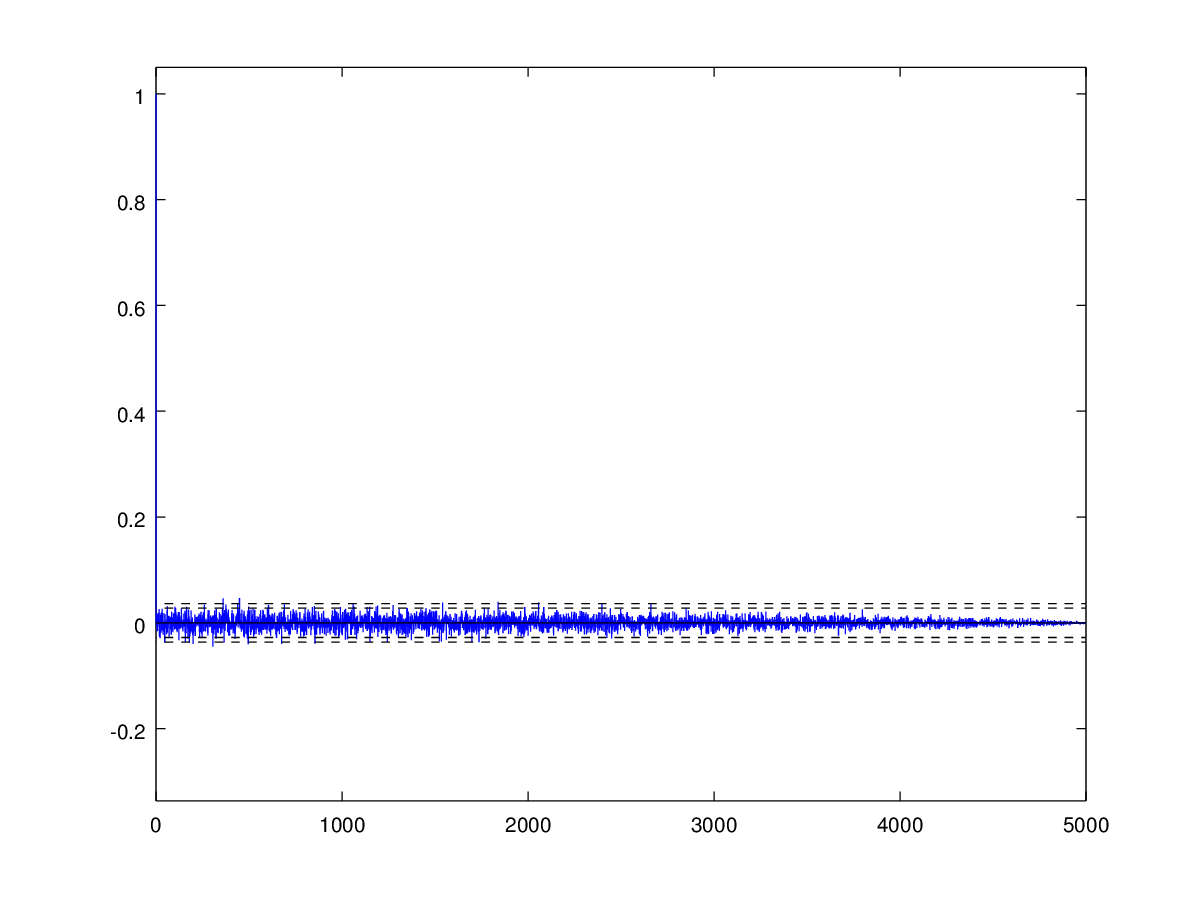
\includegraphics[width=\linewidth]{longAutocorr}
        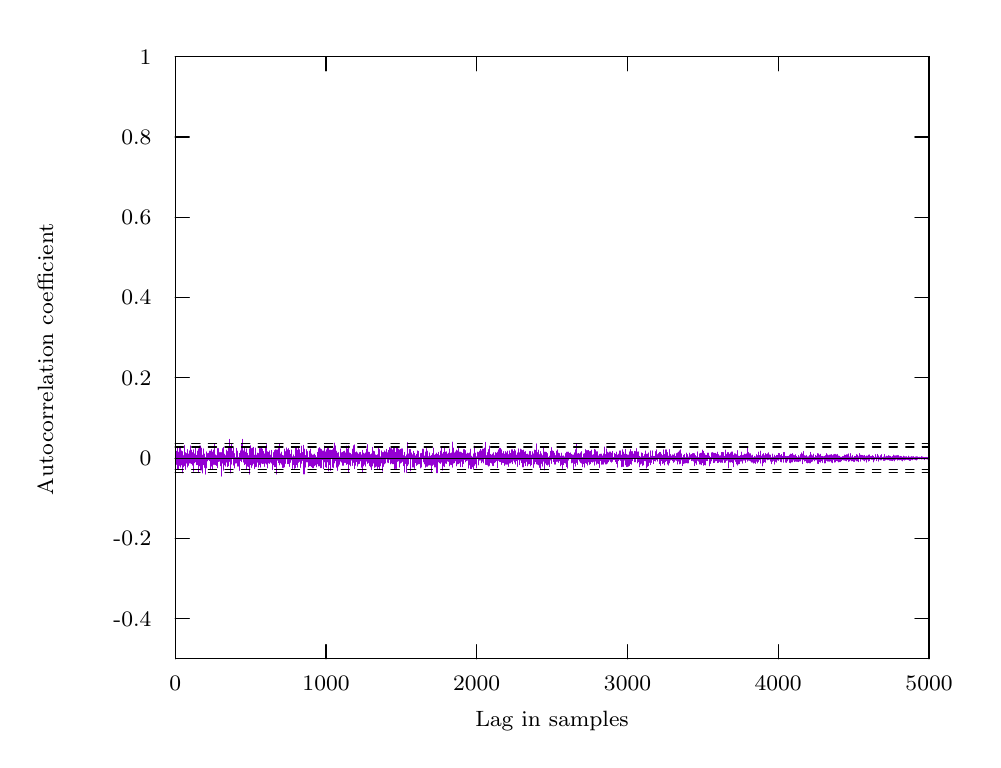
\begin{tikzpicture}[gnuplot]
%% generated with GNUPLOT 5.0p3 (Lua 5.3; terminal rev. 99, script rev. 100)
%% Mon 02 May 2016 08:45:30 BST
\path (0.000,0.000) rectangle (12.000,9.000);
\gpcolor{color=gp lt color border}
\gpsetlinetype{gp lt border}
\gpsetdashtype{gp dt solid}
\gpsetlinewidth{1.00}
\draw[gp path] (1.872,1.495)--(2.052,1.495);
\draw[gp path] (11.447,1.495)--(11.267,1.495);
\node[gp node right] at (1.688,1.495) {\footnotesize -0.4};
\draw[gp path] (1.872,2.514)--(2.052,2.514);
\draw[gp path] (11.447,2.514)--(11.267,2.514);
\node[gp node right] at (1.688,2.514) {\footnotesize -0.2};
\draw[gp path] (1.872,3.534)--(2.052,3.534);
\draw[gp path] (11.447,3.534)--(11.267,3.534);
\node[gp node right] at (1.688,3.534) {\footnotesize 0};
\draw[gp path] (1.872,4.553)--(2.052,4.553);
\draw[gp path] (11.447,4.553)--(11.267,4.553);
\node[gp node right] at (1.688,4.553) {\footnotesize 0.2};
\draw[gp path] (1.872,5.573)--(2.052,5.573);
\draw[gp path] (11.447,5.573)--(11.267,5.573);
\node[gp node right] at (1.688,5.573) {\footnotesize 0.4};
\draw[gp path] (1.872,6.592)--(2.052,6.592);
\draw[gp path] (11.447,6.592)--(11.267,6.592);
\node[gp node right] at (1.688,6.592) {\footnotesize 0.6};
\draw[gp path] (1.872,7.612)--(2.052,7.612);
\draw[gp path] (11.447,7.612)--(11.267,7.612);
\node[gp node right] at (1.688,7.612) {\footnotesize 0.8};
\draw[gp path] (1.872,8.631)--(2.052,8.631);
\draw[gp path] (11.447,8.631)--(11.267,8.631);
\node[gp node right] at (1.688,8.631) {\footnotesize 1};
\draw[gp path] (1.874,0.985)--(1.874,1.165);
\draw[gp path] (1.874,8.631)--(1.874,8.451);
\node[gp node center] at (1.874,0.677) {\footnotesize 0};
\draw[gp path] (3.789,0.985)--(3.789,1.165);
\draw[gp path] (3.789,8.631)--(3.789,8.451);
\node[gp node center] at (3.789,0.677) {\footnotesize 1000};
\draw[gp path] (5.703,0.985)--(5.703,1.165);
\draw[gp path] (5.703,8.631)--(5.703,8.451);
\node[gp node center] at (5.703,0.677) {\footnotesize 2000};
\draw[gp path] (7.618,0.985)--(7.618,1.165);
\draw[gp path] (7.618,8.631)--(7.618,8.451);
\node[gp node center] at (7.618,0.677) {\footnotesize 3000};
\draw[gp path] (9.532,0.985)--(9.532,1.165);
\draw[gp path] (9.532,8.631)--(9.532,8.451);
\node[gp node center] at (9.532,0.677) {\footnotesize 4000};
\draw[gp path] (11.447,0.985)--(11.447,1.165);
\draw[gp path] (11.447,8.631)--(11.447,8.451);
\node[gp node center] at (11.447,0.677) {\footnotesize 5000};
\draw[gp path] (1.872,8.631)--(1.872,0.985)--(11.447,0.985)--(11.447,8.631)--cycle;
\node[gp node center,rotate=-270] at (0.246,4.808) {\footnotesize Autocorrelation coefficient};
\node[gp node center] at (6.659,0.215) {\footnotesize Lag in samples};
\gpcolor{rgb color={0.580,0.000,0.827}}
\draw[gp path] (1.874,3.534)--(1.874,8.631);
\draw[gp path] (1.876,3.534)--(1.876,3.502);
\draw[gp path] (1.878,3.534)--(1.878,3.554);
\draw[gp path] (1.880,3.534)--(1.880,3.630);
\draw[gp path] (1.882,3.534)--(1.882,3.617);
\draw[gp path] (1.883,3.534)--(1.883,3.456);
\draw[gp path] (1.885,3.534)--(1.885,3.500);
\draw[gp path] (1.887,3.534)--(1.887,3.454);
\draw[gp path] (1.889,3.534)--(1.889,3.600);
\draw[gp path] (1.891,3.534)--(1.891,3.494);
\draw[gp path] (1.893,3.534)--(1.893,3.620);
\draw[gp path] (1.895,3.534)--(1.895,3.605);
\draw[gp path] (1.897,3.534)--(1.897,3.556);
\draw[gp path] (1.899,3.534)--(1.899,3.558);
\draw[gp path] (1.901,3.534)--(1.901,3.631);
\draw[gp path] (1.903,3.534)--(1.903,3.538);
\draw[gp path] (1.905,3.534)--(1.905,3.667);
\draw[gp path] (1.906,3.534)--(1.906,3.407);
\draw[gp path] (1.908,3.534)--(1.908,3.398);
\draw[gp path] (1.910,3.534)--(1.910,3.484);
\draw[gp path] (1.912,3.534)--(1.912,3.566);
\draw[gp path] (1.914,3.534)--(1.914,3.387);
\draw[gp path] (1.916,3.534)--(1.916,3.609);
\draw[gp path] (1.918,3.534)--(1.918,3.567);
\draw[gp path] (1.920,3.534)--(1.920,3.570);
\draw[gp path] (1.922,3.534)--(1.922,3.535);
\draw[gp path] (1.924,3.534)--(1.924,3.440);
\draw[gp path] (1.926,3.534)--(1.926,3.626);
\draw[gp path] (1.928,3.534)--(1.928,3.633);
\draw[gp path] (1.929,3.534)--(1.929,3.597);
\draw[gp path] (1.931,3.534)--(1.931,3.465);
\draw[gp path] (1.933,3.534)--(1.933,3.479);
\draw[gp path] (1.935,3.534)--(1.935,3.669);
\draw[gp path] (1.937,3.534)--(1.937,3.464);
\draw[gp path] (1.939,3.534)--(1.939,3.628);
\draw[gp path] (1.941,3.534)--(1.941,3.526);
\draw[gp path] (1.943,3.534)--(1.943,3.482);
\draw[gp path] (1.945,3.534)--(1.945,3.419);
\draw[gp path] (1.947,3.534)--(1.947,3.490);
\draw[gp path] (1.949,3.534)--(1.949,3.453);
\draw[gp path] (1.950,3.534)--(1.950,3.546);
\draw[gp path] (1.952,3.534)--(1.952,3.482);
\draw[gp path] (1.954,3.534)--(1.954,3.448);
\draw[gp path] (1.956,3.534)--(1.956,3.626);
\draw[gp path] (1.958,3.534)--(1.958,3.542);
\draw[gp path] (1.960,3.534)--(1.960,3.499);
\draw[gp path] (1.962,3.534)--(1.962,3.346);
\draw[gp path] (1.964,3.534)--(1.964,3.501);
\draw[gp path] (1.966,3.534)--(1.966,3.615);
\draw[gp path] (1.968,3.534)--(1.968,3.507);
\draw[gp path] (1.970,3.534)--(1.970,3.484);
\draw[gp path] (1.972,3.534)--(1.972,3.481);
\draw[gp path] (1.973,3.534)--(1.973,3.485);
\draw[gp path] (1.975,3.534)--(1.975,3.518);
\draw[gp path] (1.977,3.534)--(1.977,3.564);
\draw[gp path] (1.979,3.534)--(1.979,3.488);
\draw[gp path] (1.981,3.534)--(1.981,3.424);
\draw[gp path] (1.983,3.534)--(1.983,3.537);
\draw[gp path] (1.985,3.534)--(1.985,3.444);
\draw[gp path] (1.987,3.534)--(1.987,3.654);
\draw[gp path] (1.989,3.534)--(1.989,3.693);
\draw[gp path] (1.991,3.534)--(1.991,3.600);
\draw[gp path] (1.993,3.534)--(1.993,3.441);
\draw[gp path] (1.995,3.534)--(1.995,3.535);
\draw[gp path] (1.996,3.534)--(1.996,3.482);
\draw[gp path] (1.998,3.534)--(1.998,3.530);
\draw[gp path] (2.000,3.534)--(2.000,3.553);
\draw[gp path] (2.002,3.534)--(2.002,3.598);
\draw[gp path] (2.004,3.534)--(2.004,3.600);
\draw[gp path] (2.006,3.534)--(2.006,3.578);
\draw[gp path] (2.008,3.534)--(2.008,3.390);
\draw[gp path] (2.010,3.534)--(2.010,3.571);
\draw[gp path] (2.012,3.534)--(2.012,3.540);
\draw[gp path] (2.014,3.534)--(2.014,3.568);
\draw[gp path] (2.016,3.534)--(2.016,3.561);
\draw[gp path] (2.018,3.534)--(2.018,3.590);
\draw[gp path] (2.019,3.534)--(2.019,3.471);
\draw[gp path] (2.021,3.534)--(2.021,3.585);
\draw[gp path] (2.023,3.534)--(2.023,3.512);
\draw[gp path] (2.025,3.534)--(2.025,3.523);
\draw[gp path] (2.027,3.534)--(2.027,3.488);
\draw[gp path] (2.029,3.534)--(2.029,3.421);
\draw[gp path] (2.031,3.534)--(2.031,3.477);
\draw[gp path] (2.033,3.534)--(2.033,3.641);
\draw[gp path] (2.035,3.534)--(2.035,3.490);
\draw[gp path] (2.037,3.534)--(2.037,3.549);
\draw[gp path] (2.039,3.534)--(2.039,3.461);
\draw[gp path] (2.040,3.534)--(2.040,3.585);
\draw[gp path] (2.042,3.534)--(2.042,3.510);
\draw[gp path] (2.044,3.534)--(2.044,3.575);
\draw[gp path] (2.046,3.534)--(2.046,3.443);
\draw[gp path] (2.048,3.534)--(2.048,3.556);
\draw[gp path] (2.050,3.534)--(2.050,3.626);
\draw[gp path] (2.052,3.534)--(2.052,3.500);
\draw[gp path] (2.054,3.534)--(2.054,3.560);
\draw[gp path] (2.056,3.534)--(2.056,3.552);
\draw[gp path] (2.058,3.534)--(2.058,3.504);
\draw[gp path] (2.060,3.534)--(2.060,3.509);
\draw[gp path] (2.062,3.534)--(2.062,3.471);
\draw[gp path] (2.063,3.534)--(2.063,3.477);
\draw[gp path] (2.065,3.534)--(2.065,3.630);
\draw[gp path] (2.067,3.534)--(2.067,3.687);
\draw[gp path] (2.069,3.534)--(2.069,3.475);
\draw[gp path] (2.071,3.534)--(2.071,3.480);
\draw[gp path] (2.073,3.534)--(2.073,3.676);
\draw[gp path] (2.075,3.534)--(2.075,3.617);
\draw[gp path] (2.077,3.534)--(2.077,3.634);
\draw[gp path] (2.079,3.534)--(2.079,3.531);
\draw[gp path] (2.081,3.534)--(2.081,3.552);
\draw[gp path] (2.083,3.534)--(2.083,3.560);
\draw[gp path] (2.085,3.534)--(2.085,3.465);
\draw[gp path] (2.086,3.534)--(2.086,3.514);
\draw[gp path] (2.088,3.534)--(2.088,3.602);
\draw[gp path] (2.090,3.534)--(2.090,3.444);
\draw[gp path] (2.092,3.534)--(2.092,3.458);
\draw[gp path] (2.094,3.534)--(2.094,3.581);
\draw[gp path] (2.096,3.534)--(2.096,3.479);
\draw[gp path] (2.098,3.534)--(2.098,3.580);
\draw[gp path] (2.100,3.534)--(2.100,3.487);
\draw[gp path] (2.102,3.534)--(2.102,3.618);
\draw[gp path] (2.104,3.534)--(2.104,3.636);
\draw[gp path] (2.106,3.534)--(2.106,3.522);
\draw[gp path] (2.107,3.534)--(2.107,3.367);
\draw[gp path] (2.109,3.534)--(2.109,3.636);
\draw[gp path] (2.111,3.534)--(2.111,3.623);
\draw[gp path] (2.113,3.534)--(2.113,3.545);
\draw[gp path] (2.115,3.534)--(2.115,3.475);
\draw[gp path] (2.117,3.534)--(2.117,3.587);
\draw[gp path] (2.119,3.534)--(2.119,3.524);
\draw[gp path] (2.121,3.534)--(2.121,3.480);
\draw[gp path] (2.123,3.534)--(2.123,3.489);
\draw[gp path] (2.125,3.534)--(2.125,3.487);
\draw[gp path] (2.127,3.534)--(2.127,3.557);
\draw[gp path] (2.129,3.534)--(2.129,3.488);
\draw[gp path] (2.130,3.534)--(2.130,3.596);
\draw[gp path] (2.132,3.534)--(2.132,3.673);
\draw[gp path] (2.134,3.534)--(2.134,3.590);
\draw[gp path] (2.136,3.534)--(2.136,3.614);
\draw[gp path] (2.138,3.534)--(2.138,3.519);
\draw[gp path] (2.140,3.534)--(2.140,3.567);
\draw[gp path] (2.142,3.534)--(2.142,3.487);
\draw[gp path] (2.144,3.534)--(2.144,3.495);
\draw[gp path] (2.146,3.534)--(2.146,3.473);
\draw[gp path] (2.148,3.534)--(2.148,3.499);
\draw[gp path] (2.150,3.534)--(2.150,3.450);
\draw[gp path] (2.152,3.534)--(2.152,3.503);
\draw[gp path] (2.153,3.534)--(2.153,3.551);
\draw[gp path] (2.155,3.534)--(2.155,3.559);
\draw[gp path] (2.157,3.534)--(2.157,3.549);
\draw[gp path] (2.159,3.534)--(2.159,3.623);
\draw[gp path] (2.161,3.534)--(2.161,3.557);
\draw[gp path] (2.163,3.534)--(2.163,3.501);
\draw[gp path] (2.165,3.534)--(2.165,3.547);
\draw[gp path] (2.167,3.534)--(2.167,3.543);
\draw[gp path] (2.169,3.534)--(2.169,3.503);
\draw[gp path] (2.171,3.534)--(2.171,3.650);
\draw[gp path] (2.173,3.534)--(2.173,3.439);
\draw[gp path] (2.175,3.534)--(2.175,3.349);
\draw[gp path] (2.176,3.534)--(2.176,3.512);
\draw[gp path] (2.178,3.534)--(2.178,3.624);
\draw[gp path] (2.180,3.534)--(2.180,3.509);
\draw[gp path] (2.182,3.534)--(2.182,3.435);
\draw[gp path] (2.184,3.534)--(2.184,3.547);
\draw[gp path] (2.186,3.534)--(2.186,3.661);
\draw[gp path] (2.188,3.534)--(2.188,3.687);
\draw[gp path] (2.190,3.534)--(2.190,3.529);
\draw[gp path] (2.192,3.534)--(2.192,3.546);
\draw[gp path] (2.194,3.534)--(2.194,3.500);
\draw[gp path] (2.196,3.534)--(2.196,3.560);
\draw[gp path] (2.197,3.534)--(2.197,3.484);
\draw[gp path] (2.199,3.534)--(2.199,3.582);
\draw[gp path] (2.201,3.534)--(2.201,3.382);
\draw[gp path] (2.203,3.534)--(2.203,3.524);
\draw[gp path] (2.205,3.534)--(2.205,3.465);
\draw[gp path] (2.207,3.534)--(2.207,3.661);
\draw[gp path] (2.209,3.534)--(2.209,3.602);
\draw[gp path] (2.211,3.534)--(2.211,3.576);
\draw[gp path] (2.213,3.534)--(2.213,3.450);
\draw[gp path] (2.215,3.534)--(2.215,3.345);
\draw[gp path] (2.217,3.534)--(2.217,3.496);
\draw[gp path] (2.219,3.534)--(2.219,3.570);
\draw[gp path] (2.220,3.534)--(2.220,3.402);
\draw[gp path] (2.222,3.534)--(2.222,3.431);
\draw[gp path] (2.224,3.534)--(2.224,3.522);
\draw[gp path] (2.226,3.534)--(2.226,3.466);
\draw[gp path] (2.228,3.534)--(2.228,3.452);
\draw[gp path] (2.230,3.534)--(2.230,3.528);
\draw[gp path] (2.232,3.534)--(2.232,3.536);
\draw[gp path] (2.234,3.534)--(2.234,3.651);
\draw[gp path] (2.236,3.534)--(2.236,3.476);
\draw[gp path] (2.238,3.534)--(2.238,3.558);
\draw[gp path] (2.240,3.534)--(2.240,3.453);
\draw[gp path] (2.242,3.534)--(2.242,3.507);
\draw[gp path] (2.243,3.534)--(2.243,3.439);
\draw[gp path] (2.245,3.534)--(2.245,3.585);
\draw[gp path] (2.247,3.534)--(2.247,3.492);
\draw[gp path] (2.249,3.534)--(2.249,3.416);
\draw[gp path] (2.251,3.534)--(2.251,3.537);
\draw[gp path] (2.253,3.534)--(2.253,3.535);
\draw[gp path] (2.255,3.534)--(2.255,3.330);
\draw[gp path] (2.257,3.534)--(2.257,3.480);
\draw[gp path] (2.259,3.534)--(2.259,3.432);
\draw[gp path] (2.261,3.534)--(2.261,3.530);
\draw[gp path] (2.263,3.534)--(2.263,3.520);
\draw[gp path] (2.264,3.534)--(2.264,3.452);
\draw[gp path] (2.266,3.534)--(2.266,3.538);
\draw[gp path] (2.268,3.534)--(2.268,3.477);
\draw[gp path] (2.270,3.534)--(2.270,3.509);
\draw[gp path] (2.272,3.534)--(2.272,3.613);
\draw[gp path] (2.274,3.534)--(2.274,3.566);
\draw[gp path] (2.276,3.534)--(2.276,3.409);
\draw[gp path] (2.278,3.534)--(2.278,3.548);
\draw[gp path] (2.280,3.534)--(2.280,3.529);
\draw[gp path] (2.282,3.534)--(2.282,3.590);
\draw[gp path] (2.284,3.534)--(2.284,3.548);
\draw[gp path] (2.286,3.534)--(2.286,3.498);
\draw[gp path] (2.287,3.534)--(2.287,3.528);
\draw[gp path] (2.289,3.534)--(2.289,3.571);
\draw[gp path] (2.291,3.534)--(2.291,3.588);
\draw[gp path] (2.293,3.534)--(2.293,3.570);
\draw[gp path] (2.295,3.534)--(2.295,3.516);
\draw[gp path] (2.297,3.534)--(2.297,3.515);
\draw[gp path] (2.299,3.534)--(2.299,3.556);
\draw[gp path] (2.301,3.534)--(2.301,3.570);
\draw[gp path] (2.303,3.534)--(2.303,3.595);
\draw[gp path] (2.305,3.534)--(2.305,3.503);
\draw[gp path] (2.307,3.534)--(2.307,3.538);
\draw[gp path] (2.309,3.534)--(2.309,3.600);
\draw[gp path] (2.310,3.534)--(2.310,3.526);
\draw[gp path] (2.312,3.534)--(2.312,3.526);
\draw[gp path] (2.314,3.534)--(2.314,3.607);
\draw[gp path] (2.316,3.534)--(2.316,3.623);
\draw[gp path] (2.318,3.534)--(2.318,3.568);
\draw[gp path] (2.320,3.534)--(2.320,3.449);
\draw[gp path] (2.322,3.534)--(2.322,3.399);
\draw[gp path] (2.324,3.534)--(2.324,3.513);
\draw[gp path] (2.326,3.534)--(2.326,3.462);
\draw[gp path] (2.328,3.534)--(2.328,3.446);
\draw[gp path] (2.330,3.534)--(2.330,3.611);
\draw[gp path] (2.332,3.534)--(2.332,3.553);
\draw[gp path] (2.333,3.534)--(2.333,3.539);
\draw[gp path] (2.335,3.534)--(2.335,3.640);
\draw[gp path] (2.337,3.534)--(2.337,3.581);
\draw[gp path] (2.339,3.534)--(2.339,3.432);
\draw[gp path] (2.341,3.534)--(2.341,3.492);
\draw[gp path] (2.343,3.534)--(2.343,3.478);
\draw[gp path] (2.345,3.534)--(2.345,3.491);
\draw[gp path] (2.347,3.534)--(2.347,3.390);
\draw[gp path] (2.349,3.534)--(2.349,3.594);
\draw[gp path] (2.351,3.534)--(2.351,3.538);
\draw[gp path] (2.353,3.534)--(2.353,3.513);
\draw[gp path] (2.354,3.534)--(2.354,3.611);
\draw[gp path] (2.356,3.534)--(2.356,3.549);
\draw[gp path] (2.358,3.534)--(2.358,3.453);
\draw[gp path] (2.360,3.534)--(2.360,3.634);
\draw[gp path] (2.362,3.534)--(2.362,3.558);
\draw[gp path] (2.364,3.534)--(2.364,3.576);
\draw[gp path] (2.366,3.534)--(2.366,3.546);
\draw[gp path] (2.368,3.534)--(2.368,3.453);
\draw[gp path] (2.370,3.534)--(2.370,3.707);
\draw[gp path] (2.372,3.534)--(2.372,3.554);
\draw[gp path] (2.374,3.534)--(2.374,3.536);
\draw[gp path] (2.376,3.534)--(2.376,3.519);
\draw[gp path] (2.377,3.534)--(2.377,3.510);
\draw[gp path] (2.379,3.534)--(2.379,3.529);
\draw[gp path] (2.381,3.534)--(2.381,3.459);
\draw[gp path] (2.383,3.534)--(2.383,3.451);
\draw[gp path] (2.385,3.534)--(2.385,3.575);
\draw[gp path] (2.387,3.534)--(2.387,3.497);
\draw[gp path] (2.389,3.534)--(2.389,3.558);
\draw[gp path] (2.391,3.534)--(2.391,3.500);
\draw[gp path] (2.393,3.534)--(2.393,3.519);
\draw[gp path] (2.395,3.534)--(2.395,3.505);
\draw[gp path] (2.397,3.534)--(2.397,3.489);
\draw[gp path] (2.399,3.534)--(2.399,3.564);
\draw[gp path] (2.400,3.534)--(2.400,3.545);
\draw[gp path] (2.402,3.534)--(2.402,3.502);
\draw[gp path] (2.404,3.534)--(2.404,3.439);
\draw[gp path] (2.406,3.534)--(2.406,3.413);
\draw[gp path] (2.408,3.534)--(2.408,3.654);
\draw[gp path] (2.410,3.534)--(2.410,3.615);
\draw[gp path] (2.412,3.534)--(2.412,3.529);
\draw[gp path] (2.414,3.534)--(2.414,3.544);
\draw[gp path] (2.416,3.534)--(2.416,3.573);
\draw[gp path] (2.418,3.534)--(2.418,3.653);
\draw[gp path] (2.420,3.534)--(2.420,3.494);
\draw[gp path] (2.421,3.534)--(2.421,3.492);
\draw[gp path] (2.423,3.534)--(2.423,3.540);
\draw[gp path] (2.425,3.534)--(2.425,3.544);
\draw[gp path] (2.427,3.534)--(2.427,3.546);
\draw[gp path] (2.429,3.534)--(2.429,3.554);
\draw[gp path] (2.431,3.534)--(2.431,3.551);
\draw[gp path] (2.433,3.534)--(2.433,3.604);
\draw[gp path] (2.435,3.534)--(2.435,3.496);
\draw[gp path] (2.437,3.534)--(2.437,3.501);
\draw[gp path] (2.439,3.534)--(2.439,3.543);
\draw[gp path] (2.441,3.534)--(2.441,3.502);
\draw[gp path] (2.443,3.534)--(2.443,3.585);
\draw[gp path] (2.444,3.534)--(2.444,3.573);
\draw[gp path] (2.446,3.534)--(2.446,3.454);
\draw[gp path] (2.448,3.534)--(2.448,3.437);
\draw[gp path] (2.450,3.534)--(2.450,3.580);
\draw[gp path] (2.452,3.534)--(2.452,3.563);
\draw[gp path] (2.454,3.534)--(2.454,3.602);
\draw[gp path] (2.456,3.534)--(2.456,3.482);
\draw[gp path] (2.458,3.534)--(2.458,3.305);
\draw[gp path] (2.460,3.534)--(2.460,3.433);
\draw[gp path] (2.462,3.534)--(2.462,3.539);
\draw[gp path] (2.464,3.534)--(2.464,3.584);
\draw[gp path] (2.466,3.534)--(2.466,3.602);
\draw[gp path] (2.467,3.534)--(2.467,3.421);
\draw[gp path] (2.469,3.534)--(2.469,3.487);
\draw[gp path] (2.471,3.534)--(2.471,3.507);
\draw[gp path] (2.473,3.534)--(2.473,3.561);
\draw[gp path] (2.475,3.534)--(2.475,3.652);
\draw[gp path] (2.477,3.534)--(2.477,3.470);
\draw[gp path] (2.479,3.534)--(2.479,3.513);
\draw[gp path] (2.481,3.534)--(2.481,3.574);
\draw[gp path] (2.483,3.534)--(2.483,3.610);
\draw[gp path] (2.485,3.534)--(2.485,3.475);
\draw[gp path] (2.487,3.534)--(2.487,3.583);
\draw[gp path] (2.489,3.534)--(2.489,3.393);
\draw[gp path] (2.490,3.534)--(2.490,3.382);
\draw[gp path] (2.492,3.534)--(2.492,3.668);
\draw[gp path] (2.494,3.534)--(2.494,3.553);
\draw[gp path] (2.496,3.534)--(2.496,3.538);
\draw[gp path] (2.498,3.534)--(2.498,3.516);
\draw[gp path] (2.500,3.534)--(2.500,3.476);
\draw[gp path] (2.502,3.534)--(2.502,3.584);
\draw[gp path] (2.504,3.534)--(2.504,3.479);
\draw[gp path] (2.506,3.534)--(2.506,3.447);
\draw[gp path] (2.508,3.534)--(2.508,3.445);
\draw[gp path] (2.510,3.534)--(2.510,3.532);
\draw[gp path] (2.511,3.534)--(2.511,3.433);
\draw[gp path] (2.513,3.534)--(2.513,3.566);
\draw[gp path] (2.515,3.534)--(2.515,3.507);
\draw[gp path] (2.517,3.534)--(2.517,3.517);
\draw[gp path] (2.519,3.534)--(2.519,3.488);
\draw[gp path] (2.521,3.534)--(2.521,3.543);
\draw[gp path] (2.523,3.534)--(2.523,3.527);
\draw[gp path] (2.525,3.534)--(2.525,3.635);
\draw[gp path] (2.527,3.534)--(2.527,3.482);
\draw[gp path] (2.529,3.534)--(2.529,3.584);
\draw[gp path] (2.531,3.534)--(2.531,3.490);
\draw[gp path] (2.533,3.534)--(2.533,3.617);
\draw[gp path] (2.534,3.534)--(2.534,3.548);
\draw[gp path] (2.536,3.534)--(2.536,3.426);
\draw[gp path] (2.538,3.534)--(2.538,3.510);
\draw[gp path] (2.540,3.534)--(2.540,3.470);
\draw[gp path] (2.542,3.534)--(2.542,3.451);
\draw[gp path] (2.544,3.534)--(2.544,3.602);
\draw[gp path] (2.546,3.534)--(2.546,3.478);
\draw[gp path] (2.548,3.534)--(2.548,3.529);
\draw[gp path] (2.550,3.534)--(2.550,3.437);
\draw[gp path] (2.552,3.534)--(2.552,3.541);
\draw[gp path] (2.554,3.534)--(2.554,3.473);
\draw[gp path] (2.556,3.534)--(2.556,3.668);
\draw[gp path] (2.557,3.534)--(2.557,3.509);
\draw[gp path] (2.559,3.534)--(2.559,3.563);
\draw[gp path] (2.561,3.534)--(2.561,3.491);
\draw[gp path] (2.563,3.534)--(2.563,3.770);
\draw[gp path] (2.565,3.534)--(2.565,3.521);
\draw[gp path] (2.567,3.534)--(2.567,3.605);
\draw[gp path] (2.569,3.534)--(2.569,3.627);
\draw[gp path] (2.571,3.534)--(2.571,3.476);
\draw[gp path] (2.573,3.534)--(2.573,3.345);
\draw[gp path] (2.575,3.534)--(2.575,3.578);
\draw[gp path] (2.577,3.534)--(2.577,3.578);
\draw[gp path] (2.578,3.534)--(2.578,3.656);
\draw[gp path] (2.580,3.534)--(2.580,3.532);
\draw[gp path] (2.582,3.534)--(2.582,3.457);
\draw[gp path] (2.584,3.534)--(2.584,3.507);
\draw[gp path] (2.586,3.534)--(2.586,3.636);
\draw[gp path] (2.588,3.534)--(2.588,3.532);
\draw[gp path] (2.590,3.534)--(2.590,3.644);
\draw[gp path] (2.592,3.534)--(2.592,3.709);
\draw[gp path] (2.594,3.534)--(2.594,3.671);
\draw[gp path] (2.596,3.534)--(2.596,3.552);
\draw[gp path] (2.598,3.534)--(2.598,3.576);
\draw[gp path] (2.600,3.534)--(2.600,3.591);
\draw[gp path] (2.601,3.534)--(2.601,3.609);
\draw[gp path] (2.603,3.534)--(2.603,3.547);
\draw[gp path] (2.605,3.534)--(2.605,3.623);
\draw[gp path] (2.607,3.534)--(2.607,3.584);
\draw[gp path] (2.609,3.534)--(2.609,3.444);
\draw[gp path] (2.611,3.534)--(2.611,3.547);
\draw[gp path] (2.613,3.534)--(2.613,3.572);
\draw[gp path] (2.615,3.534)--(2.615,3.641);
\draw[gp path] (2.617,3.534)--(2.617,3.662);
\draw[gp path] (2.619,3.534)--(2.619,3.528);
\draw[gp path] (2.621,3.534)--(2.621,3.414);
\draw[gp path] (2.623,3.534)--(2.623,3.591);
\draw[gp path] (2.624,3.534)--(2.624,3.554);
\draw[gp path] (2.626,3.534)--(2.626,3.564);
\draw[gp path] (2.628,3.534)--(2.628,3.551);
\draw[gp path] (2.630,3.534)--(2.630,3.410);
\draw[gp path] (2.632,3.534)--(2.632,3.549);
\draw[gp path] (2.634,3.534)--(2.634,3.471);
\draw[gp path] (2.636,3.534)--(2.636,3.494);
\draw[gp path] (2.638,3.534)--(2.638,3.496);
\draw[gp path] (2.640,3.534)--(2.640,3.527);
\draw[gp path] (2.642,3.534)--(2.642,3.485);
\draw[gp path] (2.644,3.534)--(2.644,3.519);
\draw[gp path] (2.646,3.534)--(2.646,3.500);
\draw[gp path] (2.647,3.534)--(2.647,3.524);
\draw[gp path] (2.649,3.534)--(2.649,3.472);
\draw[gp path] (2.651,3.534)--(2.651,3.624);
\draw[gp path] (2.653,3.534)--(2.653,3.596);
\draw[gp path] (2.655,3.534)--(2.655,3.656);
\draw[gp path] (2.657,3.534)--(2.657,3.550);
\draw[gp path] (2.659,3.534)--(2.659,3.498);
\draw[gp path] (2.661,3.534)--(2.661,3.514);
\draw[gp path] (2.663,3.534)--(2.663,3.479);
\draw[gp path] (2.665,3.534)--(2.665,3.532);
\draw[gp path] (2.667,3.534)--(2.667,3.431);
\draw[gp path] (2.668,3.534)--(2.668,3.623);
\draw[gp path] (2.670,3.534)--(2.670,3.608);
\draw[gp path] (2.672,3.534)--(2.672,3.477);
\draw[gp path] (2.674,3.534)--(2.674,3.454);
\draw[gp path] (2.676,3.534)--(2.676,3.543);
\draw[gp path] (2.678,3.534)--(2.678,3.537);
\draw[gp path] (2.680,3.534)--(2.680,3.521);
\draw[gp path] (2.682,3.534)--(2.682,3.433);
\draw[gp path] (2.684,3.534)--(2.684,3.509);
\draw[gp path] (2.686,3.534)--(2.686,3.379);
\draw[gp path] (2.688,3.534)--(2.688,3.431);
\draw[gp path] (2.690,3.534)--(2.690,3.507);
\draw[gp path] (2.691,3.534)--(2.691,3.480);
\draw[gp path] (2.693,3.534)--(2.693,3.593);
\draw[gp path] (2.695,3.534)--(2.695,3.562);
\draw[gp path] (2.697,3.534)--(2.697,3.504);
\draw[gp path] (2.699,3.534)--(2.699,3.602);
\draw[gp path] (2.701,3.534)--(2.701,3.523);
\draw[gp path] (2.703,3.534)--(2.703,3.508);
\draw[gp path] (2.705,3.534)--(2.705,3.624);
\draw[gp path] (2.707,3.534)--(2.707,3.593);
\draw[gp path] (2.709,3.534)--(2.709,3.545);
\draw[gp path] (2.711,3.534)--(2.711,3.601);
\draw[gp path] (2.713,3.534)--(2.713,3.721);
\draw[gp path] (2.714,3.534)--(2.714,3.618);
\draw[gp path] (2.716,3.534)--(2.716,3.665);
\draw[gp path] (2.718,3.534)--(2.718,3.489);
\draw[gp path] (2.720,3.534)--(2.720,3.539);
\draw[gp path] (2.722,3.534)--(2.722,3.643);
\draw[gp path] (2.724,3.534)--(2.724,3.572);
\draw[gp path] (2.726,3.534)--(2.726,3.533);
\draw[gp path] (2.728,3.534)--(2.728,3.530);
\draw[gp path] (2.730,3.534)--(2.730,3.639);
\draw[gp path] (2.732,3.534)--(2.732,3.771);
\draw[gp path] (2.734,3.534)--(2.734,3.520);
\draw[gp path] (2.735,3.534)--(2.735,3.561);
\draw[gp path] (2.737,3.534)--(2.737,3.502);
\draw[gp path] (2.739,3.534)--(2.739,3.482);
\draw[gp path] (2.741,3.534)--(2.741,3.554);
\draw[gp path] (2.743,3.534)--(2.743,3.562);
\draw[gp path] (2.745,3.534)--(2.745,3.626);
\draw[gp path] (2.747,3.534)--(2.747,3.494);
\draw[gp path] (2.749,3.534)--(2.749,3.541);
\draw[gp path] (2.751,3.534)--(2.751,3.450);
\draw[gp path] (2.753,3.534)--(2.753,3.517);
\draw[gp path] (2.755,3.534)--(2.755,3.553);
\draw[gp path] (2.757,3.534)--(2.757,3.658);
\draw[gp path] (2.758,3.534)--(2.758,3.540);
\draw[gp path] (2.760,3.534)--(2.760,3.537);
\draw[gp path] (2.762,3.534)--(2.762,3.477);
\draw[gp path] (2.764,3.534)--(2.764,3.491);
\draw[gp path] (2.766,3.534)--(2.766,3.512);
\draw[gp path] (2.768,3.534)--(2.768,3.462);
\draw[gp path] (2.770,3.534)--(2.770,3.488);
\draw[gp path] (2.772,3.534)--(2.772,3.610);
\draw[gp path] (2.774,3.534)--(2.774,3.406);
\draw[gp path] (2.776,3.534)--(2.776,3.491);
\draw[gp path] (2.778,3.534)--(2.778,3.619);
\draw[gp path] (2.780,3.534)--(2.780,3.650);
\draw[gp path] (2.781,3.534)--(2.781,3.393);
\draw[gp path] (2.783,3.534)--(2.783,3.493);
\draw[gp path] (2.785,3.534)--(2.785,3.517);
\draw[gp path] (2.787,3.534)--(2.787,3.594);
\draw[gp path] (2.789,3.534)--(2.789,3.433);
\draw[gp path] (2.791,3.534)--(2.791,3.570);
\draw[gp path] (2.793,3.534)--(2.793,3.530);
\draw[gp path] (2.795,3.534)--(2.795,3.594);
\draw[gp path] (2.797,3.534)--(2.797,3.553);
\draw[gp path] (2.799,3.534)--(2.799,3.533);
\draw[gp path] (2.801,3.534)--(2.801,3.514);
\draw[gp path] (2.803,3.534)--(2.803,3.425);
\draw[gp path] (2.804,3.534)--(2.804,3.425);
\draw[gp path] (2.806,3.534)--(2.806,3.503);
\draw[gp path] (2.808,3.534)--(2.808,3.565);
\draw[gp path] (2.810,3.534)--(2.810,3.503);
\draw[gp path] (2.812,3.534)--(2.812,3.381);
\draw[gp path] (2.814,3.534)--(2.814,3.616);
\draw[gp path] (2.816,3.534)--(2.816,3.479);
\draw[gp path] (2.818,3.534)--(2.818,3.651);
\draw[gp path] (2.820,3.534)--(2.820,3.411);
\draw[gp path] (2.822,3.534)--(2.822,3.330);
\draw[gp path] (2.824,3.534)--(2.824,3.450);
\draw[gp path] (2.825,3.534)--(2.825,3.690);
\draw[gp path] (2.827,3.534)--(2.827,3.489);
\draw[gp path] (2.829,3.534)--(2.829,3.601);
\draw[gp path] (2.831,3.534)--(2.831,3.529);
\draw[gp path] (2.833,3.534)--(2.833,3.538);
\draw[gp path] (2.835,3.534)--(2.835,3.514);
\draw[gp path] (2.837,3.534)--(2.837,3.653);
\draw[gp path] (2.839,3.534)--(2.839,3.518);
\draw[gp path] (2.841,3.534)--(2.841,3.519);
\draw[gp path] (2.843,3.534)--(2.843,3.459);
\draw[gp path] (2.845,3.534)--(2.845,3.448);
\draw[gp path] (2.847,3.534)--(2.847,3.417);
\draw[gp path] (2.848,3.534)--(2.848,3.551);
\draw[gp path] (2.850,3.534)--(2.850,3.527);
\draw[gp path] (2.852,3.534)--(2.852,3.661);
\draw[gp path] (2.854,3.534)--(2.854,3.445);
\draw[gp path] (2.856,3.534)--(2.856,3.518);
\draw[gp path] (2.858,3.534)--(2.858,3.545);
\draw[gp path] (2.860,3.534)--(2.860,3.599);
\draw[gp path] (2.862,3.534)--(2.862,3.540);
\draw[gp path] (2.864,3.534)--(2.864,3.616);
\draw[gp path] (2.866,3.534)--(2.866,3.467);
\draw[gp path] (2.868,3.534)--(2.868,3.526);
\draw[gp path] (2.870,3.534)--(2.870,3.526);
\draw[gp path] (2.871,3.534)--(2.871,3.670);
\draw[gp path] (2.873,3.534)--(2.873,3.481);
\draw[gp path] (2.875,3.534)--(2.875,3.470);
\draw[gp path] (2.877,3.534)--(2.877,3.401);
\draw[gp path] (2.879,3.534)--(2.879,3.484);
\draw[gp path] (2.881,3.534)--(2.881,3.570);
\draw[gp path] (2.883,3.534)--(2.883,3.521);
\draw[gp path] (2.885,3.534)--(2.885,3.449);
\draw[gp path] (2.887,3.534)--(2.887,3.423);
\draw[gp path] (2.889,3.534)--(2.889,3.660);
\draw[gp path] (2.891,3.534)--(2.891,3.554);
\draw[gp path] (2.892,3.534)--(2.892,3.593);
\draw[gp path] (2.894,3.534)--(2.894,3.515);
\draw[gp path] (2.896,3.534)--(2.896,3.553);
\draw[gp path] (2.898,3.534)--(2.898,3.502);
\draw[gp path] (2.900,3.534)--(2.900,3.468);
\draw[gp path] (2.902,3.534)--(2.902,3.428);
\draw[gp path] (2.904,3.534)--(2.904,3.479);
\draw[gp path] (2.906,3.534)--(2.906,3.522);
\draw[gp path] (2.908,3.534)--(2.908,3.570);
\draw[gp path] (2.910,3.534)--(2.910,3.521);
\draw[gp path] (2.912,3.534)--(2.912,3.553);
\draw[gp path] (2.914,3.534)--(2.914,3.596);
\draw[gp path] (2.915,3.534)--(2.915,3.555);
\draw[gp path] (2.917,3.534)--(2.917,3.485);
\draw[gp path] (2.919,3.534)--(2.919,3.524);
\draw[gp path] (2.921,3.534)--(2.921,3.483);
\draw[gp path] (2.923,3.534)--(2.923,3.545);
\draw[gp path] (2.925,3.534)--(2.925,3.592);
\draw[gp path] (2.927,3.534)--(2.927,3.456);
\draw[gp path] (2.929,3.534)--(2.929,3.536);
\draw[gp path] (2.931,3.534)--(2.931,3.444);
\draw[gp path] (2.933,3.534)--(2.933,3.419);
\draw[gp path] (2.935,3.534)--(2.935,3.532);
\draw[gp path] (2.937,3.534)--(2.937,3.452);
\draw[gp path] (2.938,3.534)--(2.938,3.476);
\draw[gp path] (2.940,3.534)--(2.940,3.522);
\draw[gp path] (2.942,3.534)--(2.942,3.618);
\draw[gp path] (2.944,3.534)--(2.944,3.455);
\draw[gp path] (2.946,3.534)--(2.946,3.451);
\draw[gp path] (2.948,3.534)--(2.948,3.543);
\draw[gp path] (2.950,3.534)--(2.950,3.655);
\draw[gp path] (2.952,3.534)--(2.952,3.569);
\draw[gp path] (2.954,3.534)--(2.954,3.488);
\draw[gp path] (2.956,3.534)--(2.956,3.437);
\draw[gp path] (2.958,3.534)--(2.958,3.542);
\draw[gp path] (2.960,3.534)--(2.960,3.419);
\draw[gp path] (2.961,3.534)--(2.961,3.484);
\draw[gp path] (2.963,3.534)--(2.963,3.575);
\draw[gp path] (2.965,3.534)--(2.965,3.501);
\draw[gp path] (2.967,3.534)--(2.967,3.602);
\draw[gp path] (2.969,3.534)--(2.969,3.469);
\draw[gp path] (2.971,3.534)--(2.971,3.518);
\draw[gp path] (2.973,3.534)--(2.973,3.659);
\draw[gp path] (2.975,3.534)--(2.975,3.485);
\draw[gp path] (2.977,3.534)--(2.977,3.648);
\draw[gp path] (2.979,3.534)--(2.979,3.570);
\draw[gp path] (2.981,3.534)--(2.981,3.465);
\draw[gp path] (2.982,3.534)--(2.982,3.474);
\draw[gp path] (2.984,3.534)--(2.984,3.576);
\draw[gp path] (2.986,3.534)--(2.986,3.491);
\draw[gp path] (2.988,3.534)--(2.988,3.613);
\draw[gp path] (2.990,3.534)--(2.990,3.521);
\draw[gp path] (2.992,3.534)--(2.992,3.614);
\draw[gp path] (2.994,3.534)--(2.994,3.587);
\draw[gp path] (2.996,3.534)--(2.996,3.501);
\draw[gp path] (2.998,3.534)--(2.998,3.468);
\draw[gp path] (3.000,3.534)--(3.000,3.563);
\draw[gp path] (3.002,3.534)--(3.002,3.558);
\draw[gp path] (3.004,3.534)--(3.004,3.517);
\draw[gp path] (3.005,3.534)--(3.005,3.576);
\draw[gp path] (3.007,3.534)--(3.007,3.586);
\draw[gp path] (3.009,3.534)--(3.009,3.477);
\draw[gp path] (3.011,3.534)--(3.011,3.490);
\draw[gp path] (3.013,3.534)--(3.013,3.429);
\draw[gp path] (3.015,3.534)--(3.015,3.496);
\draw[gp path] (3.017,3.534)--(3.017,3.506);
\draw[gp path] (3.019,3.534)--(3.019,3.667);
\draw[gp path] (3.021,3.534)--(3.021,3.470);
\draw[gp path] (3.023,3.534)--(3.023,3.536);
\draw[gp path] (3.025,3.534)--(3.025,3.541);
\draw[gp path] (3.027,3.534)--(3.027,3.591);
\draw[gp path] (3.028,3.534)--(3.028,3.516);
\draw[gp path] (3.030,3.534)--(3.030,3.703);
\draw[gp path] (3.032,3.534)--(3.032,3.614);
\draw[gp path] (3.034,3.534)--(3.034,3.565);
\draw[gp path] (3.036,3.534)--(3.036,3.500);
\draw[gp path] (3.038,3.534)--(3.038,3.459);
\draw[gp path] (3.040,3.534)--(3.040,3.614);
\draw[gp path] (3.042,3.534)--(3.042,3.490);
\draw[gp path] (3.044,3.534)--(3.044,3.592);
\draw[gp path] (3.046,3.534)--(3.046,3.444);
\draw[gp path] (3.048,3.534)--(3.048,3.507);
\draw[gp path] (3.049,3.534)--(3.049,3.504);
\draw[gp path] (3.051,3.534)--(3.051,3.410);
\draw[gp path] (3.053,3.534)--(3.053,3.580);
\draw[gp path] (3.055,3.534)--(3.055,3.607);
\draw[gp path] (3.057,3.534)--(3.057,3.540);
\draw[gp path] (3.059,3.534)--(3.059,3.592);
\draw[gp path] (3.061,3.534)--(3.061,3.474);
\draw[gp path] (3.063,3.534)--(3.063,3.551);
\draw[gp path] (3.065,3.534)--(3.065,3.491);
\draw[gp path] (3.067,3.534)--(3.067,3.626);
\draw[gp path] (3.069,3.534)--(3.069,3.467);
\draw[gp path] (3.071,3.534)--(3.071,3.472);
\draw[gp path] (3.072,3.534)--(3.072,3.590);
\draw[gp path] (3.074,3.534)--(3.074,3.616);
\draw[gp path] (3.076,3.534)--(3.076,3.577);
\draw[gp path] (3.078,3.534)--(3.078,3.535);
\draw[gp path] (3.080,3.534)--(3.080,3.513);
\draw[gp path] (3.082,3.534)--(3.082,3.482);
\draw[gp path] (3.084,3.534)--(3.084,3.570);
\draw[gp path] (3.086,3.534)--(3.086,3.524);
\draw[gp path] (3.088,3.534)--(3.088,3.521);
\draw[gp path] (3.092,3.534)--(3.092,3.614);
\draw[gp path] (3.094,3.534)--(3.094,3.630);
\draw[gp path] (3.095,3.534)--(3.095,3.512);
\draw[gp path] (3.097,3.534)--(3.097,3.471);
\draw[gp path] (3.099,3.534)--(3.099,3.532);
\draw[gp path] (3.101,3.534)--(3.101,3.536);
\draw[gp path] (3.103,3.534)--(3.103,3.489);
\draw[gp path] (3.105,3.534)--(3.105,3.478);
\draw[gp path] (3.107,3.534)--(3.107,3.420);
\draw[gp path] (3.109,3.534)--(3.109,3.471);
\draw[gp path] (3.111,3.534)--(3.111,3.456);
\draw[gp path] (3.113,3.534)--(3.113,3.388);
\draw[gp path] (3.115,3.534)--(3.115,3.524);
\draw[gp path] (3.117,3.534)--(3.117,3.481);
\draw[gp path] (3.118,3.534)--(3.118,3.449);
\draw[gp path] (3.120,3.534)--(3.120,3.602);
\draw[gp path] (3.122,3.534)--(3.122,3.523);
\draw[gp path] (3.124,3.534)--(3.124,3.544);
\draw[gp path] (3.126,3.534)--(3.126,3.467);
\draw[gp path] (3.128,3.534)--(3.128,3.548);
\draw[gp path] (3.130,3.534)--(3.130,3.462);
\draw[gp path] (3.132,3.534)--(3.132,3.521);
\draw[gp path] (3.134,3.534)--(3.134,3.459);
\draw[gp path] (3.136,3.534)--(3.136,3.576);
\draw[gp path] (3.138,3.534)--(3.138,3.528);
\draw[gp path] (3.139,3.534)--(3.139,3.627);
\draw[gp path] (3.141,3.534)--(3.141,3.425);
\draw[gp path] (3.143,3.534)--(3.143,3.616);
\draw[gp path] (3.145,3.534)--(3.145,3.584);
\draw[gp path] (3.147,3.534)--(3.147,3.550);
\draw[gp path] (3.151,3.534)--(3.151,3.639);
\draw[gp path] (3.153,3.534)--(3.153,3.480);
\draw[gp path] (3.155,3.534)--(3.155,3.555);
\draw[gp path] (3.157,3.534)--(3.157,3.536);
\draw[gp path] (3.159,3.534)--(3.159,3.545);
\draw[gp path] (3.161,3.534)--(3.161,3.474);
\draw[gp path] (3.162,3.534)--(3.162,3.528);
\draw[gp path] (3.164,3.534)--(3.164,3.332);
\draw[gp path] (3.166,3.534)--(3.166,3.637);
\draw[gp path] (3.168,3.534)--(3.168,3.511);
\draw[gp path] (3.170,3.534)--(3.170,3.572);
\draw[gp path] (3.172,3.534)--(3.172,3.547);
\draw[gp path] (3.174,3.534)--(3.174,3.529);
\draw[gp path] (3.176,3.534)--(3.176,3.591);
\draw[gp path] (3.178,3.534)--(3.178,3.509);
\draw[gp path] (3.180,3.534)--(3.180,3.520);
\draw[gp path] (3.182,3.534)--(3.182,3.500);
\draw[gp path] (3.184,3.534)--(3.184,3.506);
\draw[gp path] (3.185,3.534)--(3.185,3.653);
\draw[gp path] (3.187,3.534)--(3.187,3.624);
\draw[gp path] (3.189,3.534)--(3.189,3.551);
\draw[gp path] (3.191,3.534)--(3.191,3.476);
\draw[gp path] (3.193,3.534)--(3.193,3.712);
\draw[gp path] (3.195,3.534)--(3.195,3.500);
\draw[gp path] (3.197,3.534)--(3.197,3.612);
\draw[gp path] (3.199,3.534)--(3.199,3.520);
\draw[gp path] (3.201,3.534)--(3.201,3.448);
\draw[gp path] (3.203,3.534)--(3.203,3.565);
\draw[gp path] (3.205,3.534)--(3.205,3.560);
\draw[gp path] (3.206,3.534)--(3.206,3.586);
\draw[gp path] (3.208,3.534)--(3.208,3.473);
\draw[gp path] (3.210,3.534)--(3.210,3.544);
\draw[gp path] (3.212,3.534)--(3.212,3.494);
\draw[gp path] (3.214,3.534)--(3.214,3.481);
\draw[gp path] (3.216,3.534)--(3.216,3.495);
\draw[gp path] (3.218,3.534)--(3.218,3.527);
\draw[gp path] (3.220,3.534)--(3.220,3.492);
\draw[gp path] (3.222,3.534)--(3.222,3.475);
\draw[gp path] (3.224,3.534)--(3.224,3.506);
\draw[gp path] (3.226,3.534)--(3.226,3.458);
\draw[gp path] (3.228,3.534)--(3.228,3.512);
\draw[gp path] (3.229,3.534)--(3.229,3.610);
\draw[gp path] (3.231,3.534)--(3.231,3.536);
\draw[gp path] (3.233,3.534)--(3.233,3.466);
\draw[gp path] (3.235,3.534)--(3.235,3.498);
\draw[gp path] (3.237,3.534)--(3.237,3.523);
\draw[gp path] (3.239,3.534)--(3.239,3.428);
\draw[gp path] (3.241,3.534)--(3.241,3.569);
\draw[gp path] (3.243,3.534)--(3.243,3.414);
\draw[gp path] (3.245,3.534)--(3.245,3.501);
\draw[gp path] (3.247,3.534)--(3.247,3.428);
\draw[gp path] (3.249,3.534)--(3.249,3.493);
\draw[gp path] (3.251,3.534)--(3.251,3.493);
\draw[gp path] (3.252,3.534)--(3.252,3.562);
\draw[gp path] (3.254,3.534)--(3.254,3.559);
\draw[gp path] (3.256,3.534)--(3.256,3.423);
\draw[gp path] (3.258,3.534)--(3.258,3.648);
\draw[gp path] (3.260,3.534)--(3.260,3.490);
\draw[gp path] (3.262,3.534)--(3.262,3.558);
\draw[gp path] (3.264,3.534)--(3.264,3.544);
\draw[gp path] (3.266,3.534)--(3.266,3.560);
\draw[gp path] (3.268,3.534)--(3.268,3.525);
\draw[gp path] (3.270,3.534)--(3.270,3.500);
\draw[gp path] (3.272,3.534)--(3.272,3.572);
\draw[gp path] (3.273,3.534)--(3.273,3.487);
\draw[gp path] (3.275,3.534)--(3.275,3.616);
\draw[gp path] (3.277,3.534)--(3.277,3.466);
\draw[gp path] (3.279,3.534)--(3.279,3.596);
\draw[gp path] (3.281,3.534)--(3.281,3.549);
\draw[gp path] (3.283,3.534)--(3.283,3.566);
\draw[gp path] (3.285,3.534)--(3.285,3.664);
\draw[gp path] (3.287,3.534)--(3.287,3.529);
\draw[gp path] (3.289,3.534)--(3.289,3.525);
\draw[gp path] (3.291,3.534)--(3.291,3.630);
\draw[gp path] (3.293,3.534)--(3.293,3.640);
\draw[gp path] (3.295,3.534)--(3.295,3.609);
\draw[gp path] (3.296,3.534)--(3.296,3.572);
\draw[gp path] (3.298,3.534)--(3.298,3.539);
\draw[gp path] (3.300,3.534)--(3.300,3.559);
\draw[gp path] (3.302,3.534)--(3.302,3.522);
\draw[gp path] (3.304,3.534)--(3.304,3.465);
\draw[gp path] (3.306,3.534)--(3.306,3.591);
\draw[gp path] (3.308,3.534)--(3.308,3.465);
\draw[gp path] (3.310,3.534)--(3.310,3.478);
\draw[gp path] (3.312,3.534)--(3.312,3.618);
\draw[gp path] (3.314,3.534)--(3.314,3.653);
\draw[gp path] (3.316,3.534)--(3.316,3.504);
\draw[gp path] (3.318,3.534)--(3.318,3.497);
\draw[gp path] (3.319,3.534)--(3.319,3.587);
\draw[gp path] (3.321,3.534)--(3.321,3.569);
\draw[gp path] (3.323,3.534)--(3.323,3.630);
\draw[gp path] (3.325,3.534)--(3.325,3.428);
\draw[gp path] (3.327,3.534)--(3.327,3.450);
\draw[gp path] (3.329,3.534)--(3.329,3.577);
\draw[gp path] (3.331,3.534)--(3.331,3.480);
\draw[gp path] (3.333,3.534)--(3.333,3.582);
\draw[gp path] (3.335,3.534)--(3.335,3.536);
\draw[gp path] (3.337,3.534)--(3.337,3.519);
\draw[gp path] (3.339,3.534)--(3.339,3.518);
\draw[gp path] (3.341,3.534)--(3.341,3.544);
\draw[gp path] (3.342,3.534)--(3.342,3.486);
\draw[gp path] (3.344,3.534)--(3.344,3.511);
\draw[gp path] (3.346,3.534)--(3.346,3.547);
\draw[gp path] (3.348,3.534)--(3.348,3.527);
\draw[gp path] (3.350,3.534)--(3.350,3.633);
\draw[gp path] (3.352,3.534)--(3.352,3.635);
\draw[gp path] (3.354,3.534)--(3.354,3.517);
\draw[gp path] (3.356,3.534)--(3.356,3.532);
\draw[gp path] (3.358,3.534)--(3.358,3.522);
\draw[gp path] (3.360,3.534)--(3.360,3.550);
\draw[gp path] (3.362,3.534)--(3.362,3.403);
\draw[gp path] (3.363,3.534)--(3.363,3.498);
\draw[gp path] (3.365,3.534)--(3.365,3.541);
\draw[gp path] (3.367,3.534)--(3.367,3.488);
\draw[gp path] (3.369,3.534)--(3.369,3.495);
\draw[gp path] (3.371,3.534)--(3.371,3.451);
\draw[gp path] (3.373,3.534)--(3.373,3.574);
\draw[gp path] (3.375,3.534)--(3.375,3.494);
\draw[gp path] (3.377,3.534)--(3.377,3.555);
\draw[gp path] (3.379,3.534)--(3.379,3.516);
\draw[gp path] (3.381,3.534)--(3.381,3.547);
\draw[gp path] (3.383,3.534)--(3.383,3.449);
\draw[gp path] (3.385,3.534)--(3.385,3.552);
\draw[gp path] (3.386,3.534)--(3.386,3.523);
\draw[gp path] (3.388,3.534)--(3.388,3.466);
\draw[gp path] (3.390,3.534)--(3.390,3.463);
\draw[gp path] (3.392,3.534)--(3.392,3.404);
\draw[gp path] (3.394,3.534)--(3.394,3.465);
\draw[gp path] (3.396,3.534)--(3.396,3.624);
\draw[gp path] (3.398,3.534)--(3.398,3.598);
\draw[gp path] (3.400,3.534)--(3.400,3.548);
\draw[gp path] (3.402,3.534)--(3.402,3.413);
\draw[gp path] (3.404,3.534)--(3.404,3.561);
\draw[gp path] (3.406,3.534)--(3.406,3.572);
\draw[gp path] (3.408,3.534)--(3.408,3.671);
\draw[gp path] (3.409,3.534)--(3.409,3.451);
\draw[gp path] (3.411,3.534)--(3.411,3.590);
\draw[gp path] (3.413,3.534)--(3.413,3.527);
\draw[gp path] (3.415,3.534)--(3.415,3.539);
\draw[gp path] (3.417,3.534)--(3.417,3.535);
\draw[gp path] (3.419,3.534)--(3.419,3.529);
\draw[gp path] (3.421,3.534)--(3.421,3.551);
\draw[gp path] (3.423,3.534)--(3.423,3.418);
\draw[gp path] (3.425,3.534)--(3.425,3.531);
\draw[gp path] (3.427,3.534)--(3.427,3.501);
\draw[gp path] (3.429,3.534)--(3.429,3.527);
\draw[gp path] (3.430,3.534)--(3.430,3.633);
\draw[gp path] (3.432,3.534)--(3.432,3.588);
\draw[gp path] (3.434,3.534)--(3.434,3.585);
\draw[gp path] (3.436,3.534)--(3.436,3.552);
\draw[gp path] (3.438,3.534)--(3.438,3.661);
\draw[gp path] (3.440,3.534)--(3.440,3.526);
\draw[gp path] (3.442,3.534)--(3.442,3.480);
\draw[gp path] (3.444,3.534)--(3.444,3.573);
\draw[gp path] (3.446,3.534)--(3.446,3.568);
\draw[gp path] (3.448,3.534)--(3.448,3.492);
\draw[gp path] (3.450,3.534)--(3.450,3.615);
\draw[gp path] (3.452,3.534)--(3.452,3.583);
\draw[gp path] (3.453,3.534)--(3.453,3.639);
\draw[gp path] (3.455,3.534)--(3.455,3.501);
\draw[gp path] (3.457,3.534)--(3.457,3.536);
\draw[gp path] (3.459,3.534)--(3.459,3.593);
\draw[gp path] (3.461,3.534)--(3.461,3.550);
\draw[gp path] (3.463,3.534)--(3.463,3.515);
\draw[gp path] (3.465,3.534)--(3.465,3.542);
\draw[gp path] (3.467,3.534)--(3.467,3.416);
\draw[gp path] (3.469,3.534)--(3.469,3.501);
\draw[gp path] (3.471,3.534)--(3.471,3.467);
\draw[gp path] (3.473,3.534)--(3.473,3.564);
\draw[gp path] (3.475,3.534)--(3.475,3.479);
\draw[gp path] (3.476,3.534)--(3.476,3.551);
\draw[gp path] (3.478,3.534)--(3.478,3.569);
\draw[gp path] (3.480,3.534)--(3.480,3.624);
\draw[gp path] (3.482,3.534)--(3.482,3.684);
\draw[gp path] (3.484,3.534)--(3.484,3.544);
\draw[gp path] (3.486,3.534)--(3.486,3.504);
\draw[gp path] (3.488,3.534)--(3.488,3.510);
\draw[gp path] (3.490,3.534)--(3.490,3.599);
\draw[gp path] (3.492,3.534)--(3.492,3.521);
\draw[gp path] (3.494,3.534)--(3.494,3.569);
\draw[gp path] (3.496,3.534)--(3.496,3.605);
\draw[gp path] (3.498,3.534)--(3.498,3.547);
\draw[gp path] (3.499,3.534)--(3.499,3.568);
\draw[gp path] (3.501,3.534)--(3.501,3.467);
\draw[gp path] (3.503,3.534)--(3.503,3.695);
\draw[gp path] (3.505,3.534)--(3.505,3.425);
\draw[gp path] (3.507,3.534)--(3.507,3.610);
\draw[gp path] (3.509,3.534)--(3.509,3.333);
\draw[gp path] (3.511,3.534)--(3.511,3.603);
\draw[gp path] (3.513,3.534)--(3.513,3.423);
\draw[gp path] (3.515,3.534)--(3.515,3.519);
\draw[gp path] (3.517,3.534)--(3.517,3.525);
\draw[gp path] (3.519,3.534)--(3.519,3.648);
\draw[gp path] (3.520,3.534)--(3.520,3.499);
\draw[gp path] (3.522,3.534)--(3.522,3.561);
\draw[gp path] (3.524,3.534)--(3.524,3.491);
\draw[gp path] (3.526,3.534)--(3.526,3.420);
\draw[gp path] (3.528,3.534)--(3.528,3.478);
\draw[gp path] (3.530,3.534)--(3.530,3.564);
\draw[gp path] (3.532,3.534)--(3.532,3.557);
\draw[gp path] (3.534,3.534)--(3.534,3.531);
\draw[gp path] (3.536,3.534)--(3.536,3.546);
\draw[gp path] (3.538,3.534)--(3.538,3.497);
\draw[gp path] (3.540,3.534)--(3.540,3.487);
\draw[gp path] (3.542,3.534)--(3.542,3.559);
\draw[gp path] (3.543,3.534)--(3.543,3.641);
\draw[gp path] (3.545,3.534)--(3.545,3.529);
\draw[gp path] (3.547,3.534)--(3.547,3.514);
\draw[gp path] (3.549,3.534)--(3.549,3.614);
\draw[gp path] (3.551,3.534)--(3.551,3.515);
\draw[gp path] (3.553,3.534)--(3.553,3.487);
\draw[gp path] (3.555,3.534)--(3.555,3.572);
\draw[gp path] (3.557,3.534)--(3.557,3.589);
\draw[gp path] (3.559,3.534)--(3.559,3.488);
\draw[gp path] (3.561,3.534)--(3.561,3.422);
\draw[gp path] (3.563,3.534)--(3.563,3.458);
\draw[gp path] (3.565,3.534)--(3.565,3.494);
\draw[gp path] (3.566,3.534)--(3.566,3.479);
\draw[gp path] (3.568,3.534)--(3.568,3.510);
\draw[gp path] (3.570,3.534)--(3.570,3.520);
\draw[gp path] (3.572,3.534)--(3.572,3.538);
\draw[gp path] (3.574,3.534)--(3.574,3.575);
\draw[gp path] (3.576,3.534)--(3.576,3.579);
\draw[gp path] (3.578,3.534)--(3.578,3.623);
\draw[gp path] (3.580,3.534)--(3.580,3.491);
\draw[gp path] (3.582,3.534)--(3.582,3.521);
\draw[gp path] (3.584,3.534)--(3.584,3.502);
\draw[gp path] (3.586,3.534)--(3.586,3.437);
\draw[gp path] (3.587,3.534)--(3.587,3.538);
\draw[gp path] (3.589,3.534)--(3.589,3.523);
\draw[gp path] (3.591,3.534)--(3.591,3.558);
\draw[gp path] (3.593,3.534)--(3.593,3.492);
\draw[gp path] (3.595,3.534)--(3.595,3.639);
\draw[gp path] (3.597,3.534)--(3.597,3.648);
\draw[gp path] (3.599,3.534)--(3.599,3.505);
\draw[gp path] (3.601,3.534)--(3.601,3.585);
\draw[gp path] (3.603,3.534)--(3.603,3.494);
\draw[gp path] (3.605,3.534)--(3.605,3.471);
\draw[gp path] (3.607,3.534)--(3.607,3.426);
\draw[gp path] (3.609,3.534)--(3.609,3.563);
\draw[gp path] (3.610,3.534)--(3.610,3.583);
\draw[gp path] (3.612,3.534)--(3.612,3.482);
\draw[gp path] (3.614,3.534)--(3.614,3.545);
\draw[gp path] (3.616,3.534)--(3.616,3.535);
\draw[gp path] (3.618,3.534)--(3.618,3.491);
\draw[gp path] (3.620,3.534)--(3.620,3.560);
\draw[gp path] (3.622,3.534)--(3.622,3.572);
\draw[gp path] (3.624,3.534)--(3.624,3.410);
\draw[gp path] (3.626,3.534)--(3.626,3.520);
\draw[gp path] (3.628,3.534)--(3.628,3.507);
\draw[gp path] (3.630,3.534)--(3.630,3.575);
\draw[gp path] (3.632,3.534)--(3.632,3.491);
\draw[gp path] (3.633,3.534)--(3.633,3.487);
\draw[gp path] (3.635,3.534)--(3.635,3.531);
\draw[gp path] (3.637,3.534)--(3.637,3.523);
\draw[gp path] (3.639,3.534)--(3.639,3.485);
\draw[gp path] (3.641,3.534)--(3.641,3.437);
\draw[gp path] (3.643,3.534)--(3.643,3.583);
\draw[gp path] (3.645,3.534)--(3.645,3.515);
\draw[gp path] (3.647,3.534)--(3.647,3.550);
\draw[gp path] (3.649,3.534)--(3.649,3.556);
\draw[gp path] (3.651,3.534)--(3.651,3.493);
\draw[gp path] (3.653,3.534)--(3.653,3.553);
\draw[gp path] (3.655,3.534)--(3.655,3.519);
\draw[gp path] (3.656,3.534)--(3.656,3.496);
\draw[gp path] (3.658,3.534)--(3.658,3.565);
\draw[gp path] (3.660,3.534)--(3.660,3.449);
\draw[gp path] (3.662,3.534)--(3.662,3.504);
\draw[gp path] (3.664,3.534)--(3.664,3.423);
\draw[gp path] (3.666,3.534)--(3.666,3.541);
\draw[gp path] (3.668,3.534)--(3.668,3.543);
\draw[gp path] (3.670,3.534)--(3.670,3.470);
\draw[gp path] (3.672,3.534)--(3.672,3.472);
\draw[gp path] (3.674,3.534)--(3.674,3.536);
\draw[gp path] (3.676,3.534)--(3.676,3.461);
\draw[gp path] (3.677,3.534)--(3.677,3.466);
\draw[gp path] (3.679,3.534)--(3.679,3.517);
\draw[gp path] (3.681,3.534)--(3.681,3.578);
\draw[gp path] (3.683,3.534)--(3.683,3.605);
\draw[gp path] (3.685,3.534)--(3.685,3.527);
\draw[gp path] (3.687,3.534)--(3.687,3.568);
\draw[gp path] (3.689,3.534)--(3.689,3.652);
\draw[gp path] (3.691,3.534)--(3.691,3.565);
\draw[gp path] (3.693,3.534)--(3.693,3.505);
\draw[gp path] (3.695,3.534)--(3.695,3.598);
\draw[gp path] (3.697,3.534)--(3.697,3.492);
\draw[gp path] (3.699,3.534)--(3.699,3.434);
\draw[gp path] (3.700,3.534)--(3.700,3.523);
\draw[gp path] (3.702,3.534)--(3.702,3.436);
\draw[gp path] (3.704,3.534)--(3.704,3.593);
\draw[gp path] (3.706,3.534)--(3.706,3.585);
\draw[gp path] (3.708,3.534)--(3.708,3.584);
\draw[gp path] (3.710,3.534)--(3.710,3.667);
\draw[gp path] (3.712,3.534)--(3.712,3.647);
\draw[gp path] (3.714,3.534)--(3.714,3.414);
\draw[gp path] (3.716,3.534)--(3.716,3.522);
\draw[gp path] (3.718,3.534)--(3.718,3.471);
\draw[gp path] (3.720,3.534)--(3.720,3.651);
\draw[gp path] (3.722,3.534)--(3.722,3.553);
\draw[gp path] (3.723,3.534)--(3.723,3.513);
\draw[gp path] (3.725,3.534)--(3.725,3.414);
\draw[gp path] (3.727,3.534)--(3.727,3.510);
\draw[gp path] (3.729,3.534)--(3.729,3.465);
\draw[gp path] (3.731,3.534)--(3.731,3.636);
\draw[gp path] (3.733,3.534)--(3.733,3.545);
\draw[gp path] (3.735,3.534)--(3.735,3.642);
\draw[gp path] (3.737,3.534)--(3.737,3.470);
\draw[gp path] (3.739,3.534)--(3.739,3.557);
\draw[gp path] (3.741,3.534)--(3.741,3.535);
\draw[gp path] (3.743,3.534)--(3.743,3.513);
\draw[gp path] (3.744,3.534)--(3.744,3.578);
\draw[gp path] (3.746,3.534)--(3.746,3.592);
\draw[gp path] (3.748,3.534)--(3.748,3.599);
\draw[gp path] (3.750,3.534)--(3.750,3.624);
\draw[gp path] (3.752,3.534)--(3.752,3.399);
\draw[gp path] (3.754,3.534)--(3.754,3.507);
\draw[gp path] (3.756,3.534)--(3.756,3.564);
\draw[gp path] (3.758,3.534)--(3.758,3.574);
\draw[gp path] (3.760,3.534)--(3.760,3.410);
\draw[gp path] (3.762,3.534)--(3.762,3.530);
\draw[gp path] (3.764,3.534)--(3.764,3.486);
\draw[gp path] (3.766,3.534)--(3.766,3.520);
\draw[gp path] (3.767,3.534)--(3.767,3.577);
\draw[gp path] (3.769,3.534)--(3.769,3.685);
\draw[gp path] (3.771,3.534)--(3.771,3.563);
\draw[gp path] (3.773,3.534)--(3.773,3.589);
\draw[gp path] (3.775,3.534)--(3.775,3.564);
\draw[gp path] (3.777,3.534)--(3.777,3.519);
\draw[gp path] (3.779,3.534)--(3.779,3.441);
\draw[gp path] (3.781,3.534)--(3.781,3.530);
\draw[gp path] (3.783,3.534)--(3.783,3.506);
\draw[gp path] (3.785,3.534)--(3.785,3.424);
\draw[gp path] (3.787,3.534)--(3.787,3.495);
\draw[gp path] (3.789,3.534)--(3.789,3.613);
\draw[gp path] (3.790,3.534)--(3.790,3.415);
\draw[gp path] (3.792,3.534)--(3.792,3.526);
\draw[gp path] (3.794,3.534)--(3.794,3.638);
\draw[gp path] (3.796,3.534)--(3.796,3.487);
\draw[gp path] (3.798,3.534)--(3.798,3.562);
\draw[gp path] (3.800,3.534)--(3.800,3.525);
\draw[gp path] (3.802,3.534)--(3.802,3.485);
\draw[gp path] (3.804,3.534)--(3.804,3.558);
\draw[gp path] (3.806,3.534)--(3.806,3.503);
\draw[gp path] (3.808,3.534)--(3.808,3.583);
\draw[gp path] (3.810,3.534)--(3.810,3.640);
\draw[gp path] (3.812,3.534)--(3.812,3.504);
\draw[gp path] (3.813,3.534)--(3.813,3.659);
\draw[gp path] (3.815,3.534)--(3.815,3.579);
\draw[gp path] (3.817,3.534)--(3.817,3.503);
\draw[gp path] (3.819,3.534)--(3.819,3.481);
\draw[gp path] (3.821,3.534)--(3.821,3.592);
\draw[gp path] (3.823,3.534)--(3.823,3.373);
\draw[gp path] (3.825,3.534)--(3.825,3.669);
\draw[gp path] (3.827,3.534)--(3.827,3.527);
\draw[gp path] (3.829,3.534)--(3.829,3.553);
\draw[gp path] (3.831,3.534)--(3.831,3.583);
\draw[gp path] (3.833,3.534)--(3.833,3.614);
\draw[gp path] (3.834,3.534)--(3.834,3.582);
\draw[gp path] (3.836,3.534)--(3.836,3.597);
\draw[gp path] (3.838,3.534)--(3.838,3.451);
\draw[gp path] (3.840,3.534)--(3.840,3.635);
\draw[gp path] (3.842,3.534)--(3.842,3.507);
\draw[gp path] (3.844,3.534)--(3.844,3.378);
\draw[gp path] (3.846,3.534)--(3.846,3.531);
\draw[gp path] (3.848,3.534)--(3.848,3.615);
\draw[gp path] (3.850,3.534)--(3.850,3.585);
\draw[gp path] (3.852,3.534)--(3.852,3.610);
\draw[gp path] (3.854,3.534)--(3.854,3.632);
\draw[gp path] (3.856,3.534)--(3.856,3.544);
\draw[gp path] (3.857,3.534)--(3.857,3.530);
\draw[gp path] (3.859,3.534)--(3.859,3.591);
\draw[gp path] (3.861,3.534)--(3.861,3.587);
\draw[gp path] (3.863,3.534)--(3.863,3.570);
\draw[gp path] (3.865,3.534)--(3.865,3.528);
\draw[gp path] (3.867,3.534)--(3.867,3.602);
\draw[gp path] (3.869,3.534)--(3.869,3.565);
\draw[gp path] (3.871,3.534)--(3.871,3.564);
\draw[gp path] (3.873,3.534)--(3.873,3.510);
\draw[gp path] (3.875,3.534)--(3.875,3.638);
\draw[gp path] (3.877,3.534)--(3.877,3.419);
\draw[gp path] (3.879,3.534)--(3.879,3.488);
\draw[gp path] (3.880,3.534)--(3.880,3.583);
\draw[gp path] (3.882,3.534)--(3.882,3.494);
\draw[gp path] (3.884,3.534)--(3.884,3.417);
\draw[gp path] (3.886,3.534)--(3.886,3.659);
\draw[gp path] (3.888,3.534)--(3.888,3.644);
\draw[gp path] (3.890,3.534)--(3.890,3.554);
\draw[gp path] (3.892,3.534)--(3.892,3.564);
\draw[gp path] (3.894,3.534)--(3.894,3.531);
\draw[gp path] (3.896,3.534)--(3.896,3.472);
\draw[gp path] (3.898,3.534)--(3.898,3.519);
\draw[gp path] (3.900,3.534)--(3.900,3.515);
\draw[gp path] (3.901,3.534)--(3.901,3.724);
\draw[gp path] (3.903,3.534)--(3.903,3.501);
\draw[gp path] (3.905,3.534)--(3.905,3.503);
\draw[gp path] (3.907,3.534)--(3.907,3.521);
\draw[gp path] (3.909,3.534)--(3.909,3.610);
\draw[gp path] (3.911,3.534)--(3.911,3.689);
\draw[gp path] (3.913,3.534)--(3.913,3.608);
\draw[gp path] (3.915,3.534)--(3.915,3.587);
\draw[gp path] (3.917,3.534)--(3.917,3.622);
\draw[gp path] (3.919,3.534)--(3.919,3.576);
\draw[gp path] (3.921,3.534)--(3.921,3.418);
\draw[gp path] (3.923,3.534)--(3.923,3.471);
\draw[gp path] (3.924,3.534)--(3.924,3.516);
\draw[gp path] (3.926,3.534)--(3.926,3.488);
\draw[gp path] (3.928,3.534)--(3.928,3.540);
\draw[gp path] (3.930,3.534)--(3.930,3.574);
\draw[gp path] (3.932,3.534)--(3.932,3.579);
\draw[gp path] (3.934,3.534)--(3.934,3.578);
\draw[gp path] (3.936,3.534)--(3.936,3.595);
\draw[gp path] (3.938,3.534)--(3.938,3.377);
\draw[gp path] (3.940,3.534)--(3.940,3.594);
\draw[gp path] (3.942,3.534)--(3.942,3.484);
\draw[gp path] (3.944,3.534)--(3.944,3.512);
\draw[gp path] (3.946,3.534)--(3.946,3.477);
\draw[gp path] (3.947,3.534)--(3.947,3.603);
\draw[gp path] (3.949,3.534)--(3.949,3.511);
\draw[gp path] (3.951,3.534)--(3.951,3.433);
\draw[gp path] (3.953,3.534)--(3.953,3.475);
\draw[gp path] (3.955,3.534)--(3.955,3.456);
\draw[gp path] (3.957,3.534)--(3.957,3.500);
\draw[gp path] (3.959,3.534)--(3.959,3.529);
\draw[gp path] (3.961,3.534)--(3.961,3.487);
\draw[gp path] (3.963,3.534)--(3.963,3.547);
\draw[gp path] (3.965,3.534)--(3.965,3.507);
\draw[gp path] (3.967,3.534)--(3.967,3.522);
\draw[gp path] (3.969,3.534)--(3.969,3.511);
\draw[gp path] (3.970,3.534)--(3.970,3.506);
\draw[gp path] (3.972,3.534)--(3.972,3.504);
\draw[gp path] (3.974,3.534)--(3.974,3.649);
\draw[gp path] (3.976,3.534)--(3.976,3.496);
\draw[gp path] (3.978,3.534)--(3.978,3.541);
\draw[gp path] (3.980,3.534)--(3.980,3.484);
\draw[gp path] (3.982,3.534)--(3.982,3.570);
\draw[gp path] (3.984,3.534)--(3.984,3.591);
\draw[gp path] (3.986,3.534)--(3.986,3.601);
\draw[gp path] (3.988,3.534)--(3.988,3.505);
\draw[gp path] (3.990,3.534)--(3.990,3.508);
\draw[gp path] (3.991,3.534)--(3.991,3.532);
\draw[gp path] (3.993,3.534)--(3.993,3.606);
\draw[gp path] (3.995,3.534)--(3.995,3.493);
\draw[gp path] (3.997,3.534)--(3.997,3.592);
\draw[gp path] (3.999,3.534)--(3.999,3.566);
\draw[gp path] (4.001,3.534)--(4.001,3.580);
\draw[gp path] (4.003,3.534)--(4.003,3.574);
\draw[gp path] (4.005,3.534)--(4.005,3.443);
\draw[gp path] (4.007,3.534)--(4.007,3.526);
\draw[gp path] (4.009,3.534)--(4.009,3.566);
\draw[gp path] (4.011,3.534)--(4.011,3.555);
\draw[gp path] (4.013,3.534)--(4.013,3.536);
\draw[gp path] (4.014,3.534)--(4.014,3.572);
\draw[gp path] (4.016,3.534)--(4.016,3.615);
\draw[gp path] (4.018,3.534)--(4.018,3.604);
\draw[gp path] (4.020,3.534)--(4.020,3.603);
\draw[gp path] (4.022,3.534)--(4.022,3.540);
\draw[gp path] (4.024,3.534)--(4.024,3.581);
\draw[gp path] (4.026,3.534)--(4.026,3.501);
\draw[gp path] (4.028,3.534)--(4.028,3.621);
\draw[gp path] (4.030,3.534)--(4.030,3.477);
\draw[gp path] (4.032,3.534)--(4.032,3.564);
\draw[gp path] (4.034,3.534)--(4.034,3.492);
\draw[gp path] (4.036,3.534)--(4.036,3.485);
\draw[gp path] (4.037,3.534)--(4.037,3.517);
\draw[gp path] (4.039,3.534)--(4.039,3.575);
\draw[gp path] (4.041,3.534)--(4.041,3.600);
\draw[gp path] (4.043,3.534)--(4.043,3.537);
\draw[gp path] (4.045,3.534)--(4.045,3.685);
\draw[gp path] (4.047,3.534)--(4.047,3.461);
\draw[gp path] (4.049,3.534)--(4.049,3.455);
\draw[gp path] (4.051,3.534)--(4.051,3.541);
\draw[gp path] (4.053,3.534)--(4.053,3.581);
\draw[gp path] (4.055,3.534)--(4.055,3.523);
\draw[gp path] (4.057,3.534)--(4.057,3.646);
\draw[gp path] (4.058,3.534)--(4.058,3.490);
\draw[gp path] (4.060,3.534)--(4.060,3.631);
\draw[gp path] (4.062,3.534)--(4.062,3.587);
\draw[gp path] (4.064,3.534)--(4.064,3.561);
\draw[gp path] (4.066,3.534)--(4.066,3.476);
\draw[gp path] (4.068,3.534)--(4.068,3.462);
\draw[gp path] (4.070,3.534)--(4.070,3.476);
\draw[gp path] (4.072,3.534)--(4.072,3.688);
\draw[gp path] (4.074,3.534)--(4.074,3.349);
\draw[gp path] (4.076,3.534)--(4.076,3.468);
\draw[gp path] (4.078,3.534)--(4.078,3.532);
\draw[gp path] (4.080,3.534)--(4.080,3.400);
\draw[gp path] (4.081,3.534)--(4.081,3.471);
\draw[gp path] (4.083,3.534)--(4.083,3.476);
\draw[gp path] (4.085,3.534)--(4.085,3.455);
\draw[gp path] (4.087,3.534)--(4.087,3.468);
\draw[gp path] (4.089,3.534)--(4.089,3.559);
\draw[gp path] (4.091,3.534)--(4.091,3.598);
\draw[gp path] (4.093,3.534)--(4.093,3.490);
\draw[gp path] (4.095,3.534)--(4.095,3.571);
\draw[gp path] (4.097,3.534)--(4.097,3.434);
\draw[gp path] (4.099,3.534)--(4.099,3.589);
\draw[gp path] (4.101,3.534)--(4.101,3.591);
\draw[gp path] (4.103,3.534)--(4.103,3.546);
\draw[gp path] (4.104,3.534)--(4.104,3.501);
\draw[gp path] (4.106,3.534)--(4.106,3.526);
\draw[gp path] (4.108,3.534)--(4.108,3.509);
\draw[gp path] (4.110,3.534)--(4.110,3.542);
\draw[gp path] (4.112,3.534)--(4.112,3.535);
\draw[gp path] (4.114,3.534)--(4.114,3.578);
\draw[gp path] (4.116,3.534)--(4.116,3.572);
\draw[gp path] (4.118,3.534)--(4.118,3.565);
\draw[gp path] (4.120,3.534)--(4.120,3.441);
\draw[gp path] (4.122,3.534)--(4.122,3.485);
\draw[gp path] (4.124,3.534)--(4.124,3.646);
\draw[gp path] (4.126,3.534)--(4.126,3.547);
\draw[gp path] (4.127,3.534)--(4.127,3.547);
\draw[gp path] (4.129,3.534)--(4.129,3.482);
\draw[gp path] (4.131,3.534)--(4.131,3.508);
\draw[gp path] (4.133,3.534)--(4.133,3.640);
\draw[gp path] (4.135,3.534)--(4.135,3.579);
\draw[gp path] (4.137,3.534)--(4.137,3.604);
\draw[gp path] (4.139,3.534)--(4.139,3.690);
\draw[gp path] (4.141,3.534)--(4.141,3.481);
\draw[gp path] (4.143,3.534)--(4.143,3.604);
\draw[gp path] (4.145,3.534)--(4.145,3.558);
\draw[gp path] (4.147,3.534)--(4.147,3.526);
\draw[gp path] (4.148,3.534)--(4.148,3.623);
\draw[gp path] (4.150,3.534)--(4.150,3.470);
\draw[gp path] (4.152,3.534)--(4.152,3.591);
\draw[gp path] (4.154,3.534)--(4.154,3.700);
\draw[gp path] (4.156,3.534)--(4.156,3.400);
\draw[gp path] (4.158,3.534)--(4.158,3.446);
\draw[gp path] (4.160,3.534)--(4.160,3.483);
\draw[gp path] (4.162,3.534)--(4.162,3.596);
\draw[gp path] (4.164,3.534)--(4.164,3.545);
\draw[gp path] (4.166,3.534)--(4.166,3.551);
\draw[gp path] (4.168,3.534)--(4.168,3.448);
\draw[gp path] (4.170,3.534)--(4.170,3.604);
\draw[gp path] (4.171,3.534)--(4.171,3.559);
\draw[gp path] (4.173,3.534)--(4.173,3.571);
\draw[gp path] (4.175,3.534)--(4.175,3.544);
\draw[gp path] (4.177,3.534)--(4.177,3.611);
\draw[gp path] (4.179,3.534)--(4.179,3.490);
\draw[gp path] (4.181,3.534)--(4.181,3.528);
\draw[gp path] (4.183,3.534)--(4.183,3.507);
\draw[gp path] (4.185,3.534)--(4.185,3.600);
\draw[gp path] (4.187,3.534)--(4.187,3.464);
\draw[gp path] (4.189,3.534)--(4.189,3.522);
\draw[gp path] (4.191,3.534)--(4.191,3.504);
\draw[gp path] (4.193,3.534)--(4.193,3.522);
\draw[gp path] (4.194,3.534)--(4.194,3.432);
\draw[gp path] (4.196,3.534)--(4.196,3.531);
\draw[gp path] (4.198,3.534)--(4.198,3.460);
\draw[gp path] (4.200,3.534)--(4.200,3.537);
\draw[gp path] (4.202,3.534)--(4.202,3.569);
\draw[gp path] (4.204,3.534)--(4.204,3.583);
\draw[gp path] (4.206,3.534)--(4.206,3.474);
\draw[gp path] (4.208,3.534)--(4.208,3.499);
\draw[gp path] (4.210,3.534)--(4.210,3.516);
\draw[gp path] (4.212,3.534)--(4.212,3.509);
\draw[gp path] (4.214,3.534)--(4.214,3.467);
\draw[gp path] (4.215,3.534)--(4.215,3.602);
\draw[gp path] (4.219,3.534)--(4.219,3.472);
\draw[gp path] (4.221,3.534)--(4.221,3.564);
\draw[gp path] (4.223,3.534)--(4.223,3.523);
\draw[gp path] (4.225,3.534)--(4.225,3.606);
\draw[gp path] (4.227,3.534)--(4.227,3.580);
\draw[gp path] (4.229,3.534)--(4.229,3.562);
\draw[gp path] (4.231,3.534)--(4.231,3.579);
\draw[gp path] (4.233,3.534)--(4.233,3.498);
\draw[gp path] (4.235,3.534)--(4.235,3.455);
\draw[gp path] (4.238,3.534)--(4.238,3.528);
\draw[gp path] (4.240,3.534)--(4.240,3.422);
\draw[gp path] (4.242,3.534)--(4.242,3.418);
\draw[gp path] (4.244,3.534)--(4.244,3.575);
\draw[gp path] (4.246,3.534)--(4.246,3.504);
\draw[gp path] (4.248,3.534)--(4.248,3.630);
\draw[gp path] (4.250,3.534)--(4.250,3.456);
\draw[gp path] (4.252,3.534)--(4.252,3.578);
\draw[gp path] (4.254,3.534)--(4.254,3.349);
\draw[gp path] (4.256,3.534)--(4.256,3.514);
\draw[gp path] (4.258,3.534)--(4.258,3.434);
\draw[gp path] (4.260,3.534)--(4.260,3.570);
\draw[gp path] (4.261,3.534)--(4.261,3.475);
\draw[gp path] (4.263,3.534)--(4.263,3.490);
\draw[gp path] (4.265,3.534)--(4.265,3.512);
\draw[gp path] (4.267,3.534)--(4.267,3.552);
\draw[gp path] (4.269,3.534)--(4.269,3.595);
\draw[gp path] (4.271,3.534)--(4.271,3.565);
\draw[gp path] (4.273,3.534)--(4.273,3.456);
\draw[gp path] (4.275,3.534)--(4.275,3.588);
\draw[gp path] (4.277,3.534)--(4.277,3.554);
\draw[gp path] (4.279,3.534)--(4.279,3.549);
\draw[gp path] (4.281,3.534)--(4.281,3.540);
\draw[gp path] (4.283,3.534)--(4.283,3.506);
\draw[gp path] (4.284,3.534)--(4.284,3.478);
\draw[gp path] (4.286,3.534)--(4.286,3.537);
\draw[gp path] (4.288,3.534)--(4.288,3.599);
\draw[gp path] (4.290,3.534)--(4.290,3.528);
\draw[gp path] (4.292,3.534)--(4.292,3.472);
\draw[gp path] (4.294,3.534)--(4.294,3.431);
\draw[gp path] (4.296,3.534)--(4.296,3.559);
\draw[gp path] (4.298,3.534)--(4.298,3.567);
\draw[gp path] (4.300,3.534)--(4.300,3.513);
\draw[gp path] (4.302,3.534)--(4.302,3.584);
\draw[gp path] (4.304,3.534)--(4.304,3.585);
\draw[gp path] (4.305,3.534)--(4.305,3.495);
\draw[gp path] (4.307,3.534)--(4.307,3.647);
\draw[gp path] (4.309,3.534)--(4.309,3.574);
\draw[gp path] (4.311,3.534)--(4.311,3.529);
\draw[gp path] (4.313,3.534)--(4.313,3.705);
\draw[gp path] (4.315,3.534)--(4.315,3.479);
\draw[gp path] (4.317,3.534)--(4.317,3.467);
\draw[gp path] (4.319,3.534)--(4.319,3.567);
\draw[gp path] (4.321,3.534)--(4.321,3.504);
\draw[gp path] (4.323,3.534)--(4.323,3.492);
\draw[gp path] (4.325,3.534)--(4.325,3.478);
\draw[gp path] (4.327,3.534)--(4.327,3.554);
\draw[gp path] (4.328,3.534)--(4.328,3.609);
\draw[gp path] (4.330,3.534)--(4.330,3.584);
\draw[gp path] (4.332,3.534)--(4.332,3.538);
\draw[gp path] (4.334,3.534)--(4.334,3.500);
\draw[gp path] (4.336,3.534)--(4.336,3.524);
\draw[gp path] (4.338,3.534)--(4.338,3.605);
\draw[gp path] (4.340,3.534)--(4.340,3.539);
\draw[gp path] (4.342,3.534)--(4.342,3.516);
\draw[gp path] (4.344,3.534)--(4.344,3.522);
\draw[gp path] (4.346,3.534)--(4.346,3.484);
\draw[gp path] (4.348,3.534)--(4.348,3.439);
\draw[gp path] (4.350,3.534)--(4.350,3.423);
\draw[gp path] (4.351,3.534)--(4.351,3.529);
\draw[gp path] (4.353,3.534)--(4.353,3.479);
\draw[gp path] (4.355,3.534)--(4.355,3.527);
\draw[gp path] (4.357,3.534)--(4.357,3.577);
\draw[gp path] (4.359,3.534)--(4.359,3.456);
\draw[gp path] (4.361,3.534)--(4.361,3.586);
\draw[gp path] (4.363,3.534)--(4.363,3.579);
\draw[gp path] (4.365,3.534)--(4.365,3.463);
\draw[gp path] (4.367,3.534)--(4.367,3.388);
\draw[gp path] (4.369,3.534)--(4.369,3.576);
\draw[gp path] (4.371,3.534)--(4.371,3.422);
\draw[gp path] (4.372,3.534)--(4.372,3.523);
\draw[gp path] (4.374,3.534)--(4.374,3.669);
\draw[gp path] (4.376,3.534)--(4.376,3.498);
\draw[gp path] (4.378,3.534)--(4.378,3.640);
\draw[gp path] (4.380,3.534)--(4.380,3.508);
\draw[gp path] (4.382,3.534)--(4.382,3.502);
\draw[gp path] (4.384,3.534)--(4.384,3.436);
\draw[gp path] (4.386,3.534)--(4.386,3.530);
\draw[gp path] (4.388,3.534)--(4.388,3.504);
\draw[gp path] (4.390,3.534)--(4.390,3.622);
\draw[gp path] (4.392,3.534)--(4.392,3.533);
\draw[gp path] (4.394,3.534)--(4.394,3.470);
\draw[gp path] (4.395,3.534)--(4.395,3.514);
\draw[gp path] (4.397,3.534)--(4.397,3.606);
\draw[gp path] (4.399,3.534)--(4.399,3.524);
\draw[gp path] (4.401,3.534)--(4.401,3.468);
\draw[gp path] (4.403,3.534)--(4.403,3.530);
\draw[gp path] (4.405,3.534)--(4.405,3.614);
\draw[gp path] (4.407,3.534)--(4.407,3.417);
\draw[gp path] (4.409,3.534)--(4.409,3.538);
\draw[gp path] (4.411,3.534)--(4.411,3.490);
\draw[gp path] (4.413,3.534)--(4.413,3.424);
\draw[gp path] (4.415,3.534)--(4.415,3.477);
\draw[gp path] (4.417,3.534)--(4.417,3.573);
\draw[gp path] (4.418,3.534)--(4.418,3.445);
\draw[gp path] (4.420,3.534)--(4.420,3.560);
\draw[gp path] (4.422,3.534)--(4.422,3.520);
\draw[gp path] (4.424,3.534)--(4.424,3.569);
\draw[gp path] (4.426,3.534)--(4.426,3.472);
\draw[gp path] (4.428,3.534)--(4.428,3.545);
\draw[gp path] (4.430,3.534)--(4.430,3.508);
\draw[gp path] (4.432,3.534)--(4.432,3.433);
\draw[gp path] (4.434,3.534)--(4.434,3.482);
\draw[gp path] (4.436,3.534)--(4.436,3.554);
\draw[gp path] (4.438,3.534)--(4.438,3.440);
\draw[gp path] (4.440,3.534)--(4.440,3.574);
\draw[gp path] (4.441,3.534)--(4.441,3.427);
\draw[gp path] (4.443,3.534)--(4.443,3.504);
\draw[gp path] (4.445,3.534)--(4.445,3.399);
\draw[gp path] (4.447,3.534)--(4.447,3.548);
\draw[gp path] (4.449,3.534)--(4.449,3.573);
\draw[gp path] (4.451,3.534)--(4.451,3.581);
\draw[gp path] (4.453,3.534)--(4.453,3.545);
\draw[gp path] (4.455,3.534)--(4.455,3.678);
\draw[gp path] (4.457,3.534)--(4.457,3.426);
\draw[gp path] (4.459,3.534)--(4.459,3.672);
\draw[gp path] (4.461,3.534)--(4.461,3.501);
\draw[gp path] (4.462,3.534)--(4.462,3.492);
\draw[gp path] (4.464,3.534)--(4.464,3.524);
\draw[gp path] (4.466,3.534)--(4.466,3.396);
\draw[gp path] (4.468,3.534)--(4.468,3.554);
\draw[gp path] (4.470,3.534)--(4.470,3.642);
\draw[gp path] (4.472,3.534)--(4.472,3.627);
\draw[gp path] (4.474,3.534)--(4.474,3.549);
\draw[gp path] (4.476,3.534)--(4.476,3.500);
\draw[gp path] (4.478,3.534)--(4.478,3.453);
\draw[gp path] (4.480,3.534)--(4.480,3.434);
\draw[gp path] (4.482,3.534)--(4.482,3.520);
\draw[gp path] (4.484,3.534)--(4.484,3.458);
\draw[gp path] (4.485,3.534)--(4.485,3.523);
\draw[gp path] (4.487,3.534)--(4.487,3.547);
\draw[gp path] (4.489,3.534)--(4.489,3.594);
\draw[gp path] (4.491,3.534)--(4.491,3.593);
\draw[gp path] (4.493,3.534)--(4.493,3.477);
\draw[gp path] (4.495,3.534)--(4.495,3.473);
\draw[gp path] (4.497,3.534)--(4.497,3.490);
\draw[gp path] (4.499,3.534)--(4.499,3.626);
\draw[gp path] (4.501,3.534)--(4.501,3.368);
\draw[gp path] (4.503,3.534)--(4.503,3.504);
\draw[gp path] (4.505,3.534)--(4.505,3.541);
\draw[gp path] (4.507,3.534)--(4.507,3.519);
\draw[gp path] (4.508,3.534)--(4.508,3.529);
\draw[gp path] (4.510,3.534)--(4.510,3.587);
\draw[gp path] (4.512,3.534)--(4.512,3.605);
\draw[gp path] (4.514,3.534)--(4.514,3.584);
\draw[gp path] (4.516,3.534)--(4.516,3.544);
\draw[gp path] (4.518,3.534)--(4.518,3.556);
\draw[gp path] (4.520,3.534)--(4.520,3.428);
\draw[gp path] (4.522,3.534)--(4.522,3.561);
\draw[gp path] (4.524,3.534)--(4.524,3.447);
\draw[gp path] (4.526,3.534)--(4.526,3.523);
\draw[gp path] (4.528,3.534)--(4.528,3.461);
\draw[gp path] (4.529,3.534)--(4.529,3.552);
\draw[gp path] (4.531,3.534)--(4.531,3.575);
\draw[gp path] (4.533,3.534)--(4.533,3.626);
\draw[gp path] (4.535,3.534)--(4.535,3.557);
\draw[gp path] (4.537,3.534)--(4.537,3.595);
\draw[gp path] (4.539,3.534)--(4.539,3.565);
\draw[gp path] (4.541,3.534)--(4.541,3.597);
\draw[gp path] (4.543,3.534)--(4.543,3.552);
\draw[gp path] (4.545,3.534)--(4.545,3.501);
\draw[gp path] (4.547,3.534)--(4.547,3.472);
\draw[gp path] (4.549,3.534)--(4.549,3.563);
\draw[gp path] (4.551,3.534)--(4.551,3.612);
\draw[gp path] (4.552,3.534)--(4.552,3.591);
\draw[gp path] (4.554,3.534)--(4.554,3.645);
\draw[gp path] (4.556,3.534)--(4.556,3.589);
\draw[gp path] (4.558,3.534)--(4.558,3.538);
\draw[gp path] (4.560,3.534)--(4.560,3.574);
\draw[gp path] (4.562,3.534)--(4.562,3.525);
\draw[gp path] (4.564,3.534)--(4.564,3.561);
\draw[gp path] (4.566,3.534)--(4.566,3.521);
\draw[gp path] (4.568,3.534)--(4.568,3.592);
\draw[gp path] (4.570,3.534)--(4.570,3.482);
\draw[gp path] (4.572,3.534)--(4.572,3.601);
\draw[gp path] (4.574,3.534)--(4.574,3.588);
\draw[gp path] (4.575,3.534)--(4.575,3.487);
\draw[gp path] (4.577,3.534)--(4.577,3.493);
\draw[gp path] (4.579,3.534)--(4.579,3.530);
\draw[gp path] (4.581,3.534)--(4.581,3.538);
\draw[gp path] (4.583,3.534)--(4.583,3.490);
\draw[gp path] (4.585,3.534)--(4.585,3.476);
\draw[gp path] (4.587,3.534)--(4.587,3.631);
\draw[gp path] (4.589,3.534)--(4.589,3.551);
\draw[gp path] (4.591,3.534)--(4.591,3.526);
\draw[gp path] (4.593,3.534)--(4.593,3.594);
\draw[gp path] (4.595,3.534)--(4.595,3.623);
\draw[gp path] (4.597,3.534)--(4.597,3.518);
\draw[gp path] (4.598,3.534)--(4.598,3.665);
\draw[gp path] (4.600,3.534)--(4.600,3.605);
\draw[gp path] (4.602,3.534)--(4.602,3.541);
\draw[gp path] (4.604,3.534)--(4.604,3.541);
\draw[gp path] (4.606,3.534)--(4.606,3.627);
\draw[gp path] (4.608,3.534)--(4.608,3.460);
\draw[gp path] (4.610,3.534)--(4.610,3.506);
\draw[gp path] (4.612,3.534)--(4.612,3.508);
\draw[gp path] (4.614,3.534)--(4.614,3.655);
\draw[gp path] (4.616,3.534)--(4.616,3.535);
\draw[gp path] (4.618,3.534)--(4.618,3.601);
\draw[gp path] (4.619,3.534)--(4.619,3.502);
\draw[gp path] (4.621,3.534)--(4.621,3.497);
\draw[gp path] (4.623,3.534)--(4.623,3.473);
\draw[gp path] (4.625,3.534)--(4.625,3.474);
\draw[gp path] (4.627,3.534)--(4.627,3.505);
\draw[gp path] (4.629,3.534)--(4.629,3.597);
\draw[gp path] (4.631,3.534)--(4.631,3.541);
\draw[gp path] (4.633,3.534)--(4.633,3.638);
\draw[gp path] (4.635,3.534)--(4.635,3.564);
\draw[gp path] (4.637,3.534)--(4.637,3.474);
\draw[gp path] (4.639,3.534)--(4.639,3.462);
\draw[gp path] (4.641,3.534)--(4.641,3.585);
\draw[gp path] (4.642,3.534)--(4.642,3.502);
\draw[gp path] (4.644,3.534)--(4.644,3.514);
\draw[gp path] (4.646,3.534)--(4.646,3.479);
\draw[gp path] (4.648,3.534)--(4.648,3.640);
\draw[gp path] (4.650,3.534)--(4.650,3.498);
\draw[gp path] (4.652,3.534)--(4.652,3.674);
\draw[gp path] (4.654,3.534)--(4.654,3.510);
\draw[gp path] (4.656,3.534)--(4.656,3.509);
\draw[gp path] (4.658,3.534)--(4.658,3.401);
\draw[gp path] (4.660,3.534)--(4.660,3.589);
\draw[gp path] (4.662,3.534)--(4.662,3.549);
\draw[gp path] (4.664,3.534)--(4.664,3.614);
\draw[gp path] (4.665,3.534)--(4.665,3.533);
\draw[gp path] (4.667,3.534)--(4.667,3.474);
\draw[gp path] (4.669,3.534)--(4.669,3.537);
\draw[gp path] (4.671,3.534)--(4.671,3.606);
\draw[gp path] (4.673,3.534)--(4.673,3.466);
\draw[gp path] (4.675,3.534)--(4.675,3.451);
\draw[gp path] (4.677,3.534)--(4.677,3.402);
\draw[gp path] (4.679,3.534)--(4.679,3.630);
\draw[gp path] (4.681,3.534)--(4.681,3.406);
\draw[gp path] (4.683,3.534)--(4.683,3.524);
\draw[gp path] (4.685,3.534)--(4.685,3.572);
\draw[gp path] (4.686,3.534)--(4.686,3.415);
\draw[gp path] (4.688,3.534)--(4.688,3.508);
\draw[gp path] (4.690,3.534)--(4.690,3.660);
\draw[gp path] (4.692,3.534)--(4.692,3.549);
\draw[gp path] (4.694,3.534)--(4.694,3.491);
\draw[gp path] (4.696,3.534)--(4.696,3.635);
\draw[gp path] (4.698,3.534)--(4.698,3.578);
\draw[gp path] (4.700,3.534)--(4.700,3.527);
\draw[gp path] (4.702,3.534)--(4.702,3.507);
\draw[gp path] (4.704,3.534)--(4.704,3.499);
\draw[gp path] (4.706,3.534)--(4.706,3.608);
\draw[gp path] (4.708,3.534)--(4.708,3.635);
\draw[gp path] (4.709,3.534)--(4.709,3.597);
\draw[gp path] (4.711,3.534)--(4.711,3.561);
\draw[gp path] (4.713,3.534)--(4.713,3.648);
\draw[gp path] (4.715,3.534)--(4.715,3.577);
\draw[gp path] (4.717,3.534)--(4.717,3.530);
\draw[gp path] (4.719,3.534)--(4.719,3.467);
\draw[gp path] (4.721,3.534)--(4.721,3.419);
\draw[gp path] (4.723,3.534)--(4.723,3.586);
\draw[gp path] (4.725,3.534)--(4.725,3.506);
\draw[gp path] (4.727,3.534)--(4.727,3.504);
\draw[gp path] (4.729,3.534)--(4.729,3.637);
\draw[gp path] (4.731,3.534)--(4.731,3.644);
\draw[gp path] (4.732,3.534)--(4.732,3.610);
\draw[gp path] (4.734,3.534)--(4.734,3.640);
\draw[gp path] (4.736,3.534)--(4.736,3.545);
\draw[gp path] (4.738,3.534)--(4.738,3.471);
\draw[gp path] (4.740,3.534)--(4.740,3.570);
\draw[gp path] (4.742,3.534)--(4.742,3.479);
\draw[gp path] (4.744,3.534)--(4.744,3.538);
\draw[gp path] (4.746,3.534)--(4.746,3.562);
\draw[gp path] (4.748,3.534)--(4.748,3.633);
\draw[gp path] (4.750,3.534)--(4.750,3.492);
\draw[gp path] (4.752,3.534)--(4.752,3.545);
\draw[gp path] (4.753,3.534)--(4.753,3.650);
\draw[gp path] (4.755,3.534)--(4.755,3.649);
\draw[gp path] (4.757,3.534)--(4.757,3.590);
\draw[gp path] (4.759,3.534)--(4.759,3.517);
\draw[gp path] (4.761,3.534)--(4.761,3.642);
\draw[gp path] (4.763,3.534)--(4.763,3.522);
\draw[gp path] (4.765,3.534)--(4.765,3.493);
\draw[gp path] (4.767,3.534)--(4.767,3.543);
\draw[gp path] (4.769,3.534)--(4.769,3.439);
\draw[gp path] (4.771,3.534)--(4.771,3.510);
\draw[gp path] (4.773,3.534)--(4.773,3.566);
\draw[gp path] (4.775,3.534)--(4.775,3.513);
\draw[gp path] (4.776,3.534)--(4.776,3.536);
\draw[gp path] (4.778,3.534)--(4.778,3.497);
\draw[gp path] (4.780,3.534)--(4.780,3.518);
\draw[gp path] (4.782,3.534)--(4.782,3.481);
\draw[gp path] (4.784,3.534)--(4.784,3.541);
\draw[gp path] (4.786,3.534)--(4.786,3.480);
\draw[gp path] (4.788,3.534)--(4.788,3.605);
\draw[gp path] (4.790,3.534)--(4.790,3.357);
\draw[gp path] (4.792,3.534)--(4.792,3.486);
\draw[gp path] (4.794,3.534)--(4.794,3.552);
\draw[gp path] (4.796,3.534)--(4.796,3.528);
\draw[gp path] (4.798,3.534)--(4.798,3.467);
\draw[gp path] (4.799,3.534)--(4.799,3.499);
\draw[gp path] (4.801,3.534)--(4.801,3.470);
\draw[gp path] (4.803,3.534)--(4.803,3.522);
\draw[gp path] (4.805,3.534)--(4.805,3.532);
\draw[gp path] (4.807,3.534)--(4.807,3.491);
\draw[gp path] (4.809,3.534)--(4.809,3.562);
\draw[gp path] (4.811,3.534)--(4.811,3.353);
\draw[gp path] (4.813,3.534)--(4.813,3.488);
\draw[gp path] (4.815,3.534)--(4.815,3.573);
\draw[gp path] (4.817,3.534)--(4.817,3.518);
\draw[gp path] (4.819,3.534)--(4.819,3.568);
\draw[gp path] (4.821,3.534)--(4.821,3.537);
\draw[gp path] (4.822,3.534)--(4.822,3.729);
\draw[gp path] (4.824,3.534)--(4.824,3.593);
\draw[gp path] (4.826,3.534)--(4.826,3.442);
\draw[gp path] (4.828,3.534)--(4.828,3.437);
\draw[gp path] (4.830,3.534)--(4.830,3.566);
\draw[gp path] (4.832,3.534)--(4.832,3.459);
\draw[gp path] (4.834,3.534)--(4.834,3.464);
\draw[gp path] (4.836,3.534)--(4.836,3.494);
\draw[gp path] (4.838,3.534)--(4.838,3.581);
\draw[gp path] (4.840,3.534)--(4.840,3.565);
\draw[gp path] (4.843,3.534)--(4.843,3.587);
\draw[gp path] (4.845,3.534)--(4.845,3.575);
\draw[gp path] (4.847,3.534)--(4.847,3.614);
\draw[gp path] (4.849,3.534)--(4.849,3.577);
\draw[gp path] (4.851,3.534)--(4.851,3.530);
\draw[gp path] (4.853,3.534)--(4.853,3.545);
\draw[gp path] (4.855,3.534)--(4.855,3.643);
\draw[gp path] (4.857,3.534)--(4.857,3.593);
\draw[gp path] (4.859,3.534)--(4.859,3.560);
\draw[gp path] (4.861,3.534)--(4.861,3.459);
\draw[gp path] (4.863,3.534)--(4.863,3.372);
\draw[gp path] (4.865,3.534)--(4.865,3.541);
\draw[gp path] (4.866,3.534)--(4.866,3.608);
\draw[gp path] (4.868,3.534)--(4.868,3.527);
\draw[gp path] (4.870,3.534)--(4.870,3.524);
\draw[gp path] (4.874,3.534)--(4.874,3.526);
\draw[gp path] (4.876,3.534)--(4.876,3.598);
\draw[gp path] (4.878,3.534)--(4.878,3.583);
\draw[gp path] (4.880,3.534)--(4.880,3.526);
\draw[gp path] (4.882,3.534)--(4.882,3.513);
\draw[gp path] (4.884,3.534)--(4.884,3.560);
\draw[gp path] (4.886,3.534)--(4.886,3.572);
\draw[gp path] (4.888,3.534)--(4.888,3.487);
\draw[gp path] (4.889,3.534)--(4.889,3.494);
\draw[gp path] (4.891,3.534)--(4.891,3.574);
\draw[gp path] (4.893,3.534)--(4.893,3.420);
\draw[gp path] (4.895,3.534)--(4.895,3.498);
\draw[gp path] (4.897,3.534)--(4.897,3.486);
\draw[gp path] (4.899,3.534)--(4.899,3.618);
\draw[gp path] (4.901,3.534)--(4.901,3.489);
\draw[gp path] (4.903,3.534)--(4.903,3.563);
\draw[gp path] (4.905,3.534)--(4.905,3.519);
\draw[gp path] (4.907,3.534)--(4.907,3.463);
\draw[gp path] (4.909,3.534)--(4.909,3.496);
\draw[gp path] (4.910,3.534)--(4.910,3.592);
\draw[gp path] (4.912,3.534)--(4.912,3.403);
\draw[gp path] (4.914,3.534)--(4.914,3.499);
\draw[gp path] (4.916,3.534)--(4.916,3.510);
\draw[gp path] (4.918,3.534)--(4.918,3.497);
\draw[gp path] (4.920,3.534)--(4.920,3.558);
\draw[gp path] (4.922,3.534)--(4.922,3.555);
\draw[gp path] (4.924,3.534)--(4.924,3.477);
\draw[gp path] (4.926,3.534)--(4.926,3.502);
\draw[gp path] (4.928,3.534)--(4.928,3.495);
\draw[gp path] (4.930,3.534)--(4.930,3.547);
\draw[gp path] (4.932,3.534)--(4.932,3.561);
\draw[gp path] (4.933,3.534)--(4.933,3.559);
\draw[gp path] (4.935,3.534)--(4.935,3.465);
\draw[gp path] (4.937,3.534)--(4.937,3.580);
\draw[gp path] (4.939,3.534)--(4.939,3.508);
\draw[gp path] (4.941,3.534)--(4.941,3.511);
\draw[gp path] (4.943,3.534)--(4.943,3.441);
\draw[gp path] (4.945,3.534)--(4.945,3.453);
\draw[gp path] (4.947,3.534)--(4.947,3.470);
\draw[gp path] (4.949,3.534)--(4.949,3.547);
\draw[gp path] (4.951,3.534)--(4.951,3.624);
\draw[gp path] (4.953,3.534)--(4.953,3.552);
\draw[gp path] (4.955,3.534)--(4.955,3.471);
\draw[gp path] (4.956,3.534)--(4.956,3.482);
\draw[gp path] (4.958,3.534)--(4.958,3.549);
\draw[gp path] (4.960,3.534)--(4.960,3.525);
\draw[gp path] (4.962,3.534)--(4.962,3.463);
\draw[gp path] (4.964,3.534)--(4.964,3.477);
\draw[gp path] (4.966,3.534)--(4.966,3.618);
\draw[gp path] (4.968,3.534)--(4.968,3.572);
\draw[gp path] (4.970,3.534)--(4.970,3.462);
\draw[gp path] (4.972,3.534)--(4.972,3.519);
\draw[gp path] (4.974,3.534)--(4.974,3.500);
\draw[gp path] (4.976,3.534)--(4.976,3.497);
\draw[gp path] (4.978,3.534)--(4.978,3.492);
\draw[gp path] (4.979,3.534)--(4.979,3.471);
\draw[gp path] (4.981,3.534)--(4.981,3.542);
\draw[gp path] (4.983,3.534)--(4.983,3.524);
\draw[gp path] (4.985,3.534)--(4.985,3.540);
\draw[gp path] (4.987,3.534)--(4.987,3.508);
\draw[gp path] (4.989,3.534)--(4.989,3.411);
\draw[gp path] (4.991,3.534)--(4.991,3.543);
\draw[gp path] (4.993,3.534)--(4.993,3.591);
\draw[gp path] (4.995,3.534)--(4.995,3.468);
\draw[gp path] (4.997,3.534)--(4.997,3.518);
\draw[gp path] (4.999,3.534)--(4.999,3.457);
\draw[gp path] (5.000,3.534)--(5.000,3.475);
\draw[gp path] (5.002,3.534)--(5.002,3.421);
\draw[gp path] (5.004,3.534)--(5.004,3.517);
\draw[gp path] (5.006,3.534)--(5.006,3.547);
\draw[gp path] (5.008,3.534)--(5.008,3.594);
\draw[gp path] (5.010,3.534)--(5.010,3.527);
\draw[gp path] (5.012,3.534)--(5.012,3.553);
\draw[gp path] (5.014,3.534)--(5.014,3.536);
\draw[gp path] (5.016,3.534)--(5.016,3.636);
\draw[gp path] (5.018,3.534)--(5.018,3.533);
\draw[gp path] (5.020,3.534)--(5.020,3.648);
\draw[gp path] (5.022,3.534)--(5.022,3.537);
\draw[gp path] (5.023,3.534)--(5.023,3.622);
\draw[gp path] (5.025,3.534)--(5.025,3.485);
\draw[gp path] (5.027,3.534)--(5.027,3.571);
\draw[gp path] (5.029,3.534)--(5.029,3.503);
\draw[gp path] (5.031,3.534)--(5.031,3.522);
\draw[gp path] (5.033,3.534)--(5.033,3.539);
\draw[gp path] (5.035,3.534)--(5.035,3.557);
\draw[gp path] (5.037,3.534)--(5.037,3.510);
\draw[gp path] (5.039,3.534)--(5.039,3.462);
\draw[gp path] (5.041,3.534)--(5.041,3.507);
\draw[gp path] (5.045,3.534)--(5.045,3.472);
\draw[gp path] (5.046,3.534)--(5.046,3.557);
\draw[gp path] (5.048,3.534)--(5.048,3.513);
\draw[gp path] (5.050,3.534)--(5.050,3.589);
\draw[gp path] (5.052,3.534)--(5.052,3.578);
\draw[gp path] (5.054,3.534)--(5.054,3.552);
\draw[gp path] (5.056,3.534)--(5.056,3.418);
\draw[gp path] (5.058,3.534)--(5.058,3.611);
\draw[gp path] (5.060,3.534)--(5.060,3.638);
\draw[gp path] (5.062,3.534)--(5.062,3.510);
\draw[gp path] (5.064,3.534)--(5.064,3.527);
\draw[gp path] (5.066,3.534)--(5.066,3.522);
\draw[gp path] (5.067,3.534)--(5.067,3.654);
\draw[gp path] (5.069,3.534)--(5.069,3.565);
\draw[gp path] (5.071,3.534)--(5.071,3.429);
\draw[gp path] (5.073,3.534)--(5.073,3.541);
\draw[gp path] (5.075,3.534)--(5.075,3.552);
\draw[gp path] (5.077,3.534)--(5.077,3.621);
\draw[gp path] (5.079,3.534)--(5.079,3.608);
\draw[gp path] (5.081,3.534)--(5.081,3.439);
\draw[gp path] (5.083,3.534)--(5.083,3.587);
\draw[gp path] (5.085,3.534)--(5.085,3.498);
\draw[gp path] (5.087,3.534)--(5.087,3.491);
\draw[gp path] (5.089,3.534)--(5.089,3.519);
\draw[gp path] (5.090,3.534)--(5.090,3.553);
\draw[gp path] (5.092,3.534)--(5.092,3.470);
\draw[gp path] (5.094,3.534)--(5.094,3.464);
\draw[gp path] (5.096,3.534)--(5.096,3.445);
\draw[gp path] (5.098,3.534)--(5.098,3.561);
\draw[gp path] (5.100,3.534)--(5.100,3.519);
\draw[gp path] (5.102,3.534)--(5.102,3.449);
\draw[gp path] (5.104,3.534)--(5.104,3.472);
\draw[gp path] (5.106,3.534)--(5.106,3.600);
\draw[gp path] (5.108,3.534)--(5.108,3.543);
\draw[gp path] (5.110,3.534)--(5.110,3.559);
\draw[gp path] (5.112,3.534)--(5.112,3.503);
\draw[gp path] (5.113,3.534)--(5.113,3.547);
\draw[gp path] (5.115,3.534)--(5.115,3.530);
\draw[gp path] (5.117,3.534)--(5.117,3.489);
\draw[gp path] (5.119,3.534)--(5.119,3.445);
\draw[gp path] (5.121,3.534)--(5.121,3.545);
\draw[gp path] (5.123,3.534)--(5.123,3.567);
\draw[gp path] (5.125,3.534)--(5.125,3.351);
\draw[gp path] (5.127,3.534)--(5.127,3.505);
\draw[gp path] (5.129,3.534)--(5.129,3.554);
\draw[gp path] (5.131,3.534)--(5.131,3.552);
\draw[gp path] (5.133,3.534)--(5.133,3.563);
\draw[gp path] (5.135,3.534)--(5.135,3.450);
\draw[gp path] (5.136,3.534)--(5.136,3.463);
\draw[gp path] (5.138,3.534)--(5.138,3.450);
\draw[gp path] (5.140,3.534)--(5.140,3.591);
\draw[gp path] (5.142,3.534)--(5.142,3.537);
\draw[gp path] (5.144,3.534)--(5.144,3.491);
\draw[gp path] (5.146,3.534)--(5.146,3.440);
\draw[gp path] (5.148,3.534)--(5.148,3.568);
\draw[gp path] (5.150,3.534)--(5.150,3.507);
\draw[gp path] (5.152,3.534)--(5.152,3.603);
\draw[gp path] (5.154,3.534)--(5.154,3.518);
\draw[gp path] (5.156,3.534)--(5.156,3.505);
\draw[gp path] (5.157,3.534)--(5.157,3.454);
\draw[gp path] (5.159,3.534)--(5.159,3.659);
\draw[gp path] (5.161,3.534)--(5.161,3.470);
\draw[gp path] (5.163,3.534)--(5.163,3.571);
\draw[gp path] (5.165,3.534)--(5.165,3.529);
\draw[gp path] (5.167,3.534)--(5.167,3.493);
\draw[gp path] (5.169,3.534)--(5.169,3.518);
\draw[gp path] (5.171,3.534)--(5.171,3.536);
\draw[gp path] (5.173,3.534)--(5.173,3.421);
\draw[gp path] (5.175,3.534)--(5.175,3.499);
\draw[gp path] (5.177,3.534)--(5.177,3.455);
\draw[gp path] (5.179,3.534)--(5.179,3.486);
\draw[gp path] (5.180,3.534)--(5.180,3.579);
\draw[gp path] (5.182,3.534)--(5.182,3.559);
\draw[gp path] (5.184,3.534)--(5.184,3.526);
\draw[gp path] (5.186,3.534)--(5.186,3.516);
\draw[gp path] (5.188,3.534)--(5.188,3.515);
\draw[gp path] (5.190,3.534)--(5.190,3.445);
\draw[gp path] (5.192,3.534)--(5.192,3.560);
\draw[gp path] (5.194,3.534)--(5.194,3.597);
\draw[gp path] (5.196,3.534)--(5.196,3.529);
\draw[gp path] (5.198,3.534)--(5.198,3.348);
\draw[gp path] (5.200,3.534)--(5.200,3.581);
\draw[gp path] (5.202,3.534)--(5.202,3.570);
\draw[gp path] (5.203,3.534)--(5.203,3.486);
\draw[gp path] (5.205,3.534)--(5.205,3.541);
\draw[gp path] (5.207,3.534)--(5.207,3.456);
\draw[gp path] (5.211,3.534)--(5.211,3.537);
\draw[gp path] (5.213,3.534)--(5.213,3.597);
\draw[gp path] (5.215,3.534)--(5.215,3.577);
\draw[gp path] (5.217,3.534)--(5.217,3.606);
\draw[gp path] (5.219,3.534)--(5.219,3.533);
\draw[gp path] (5.221,3.534)--(5.221,3.485);
\draw[gp path] (5.223,3.534)--(5.223,3.551);
\draw[gp path] (5.224,3.534)--(5.224,3.530);
\draw[gp path] (5.226,3.534)--(5.226,3.475);
\draw[gp path] (5.228,3.534)--(5.228,3.477);
\draw[gp path] (5.230,3.534)--(5.230,3.565);
\draw[gp path] (5.232,3.534)--(5.232,3.525);
\draw[gp path] (5.234,3.534)--(5.234,3.545);
\draw[gp path] (5.236,3.534)--(5.236,3.538);
\draw[gp path] (5.238,3.534)--(5.238,3.498);
\draw[gp path] (5.240,3.534)--(5.240,3.467);
\draw[gp path] (5.242,3.534)--(5.242,3.522);
\draw[gp path] (5.244,3.534)--(5.244,3.492);
\draw[gp path] (5.246,3.534)--(5.246,3.594);
\draw[gp path] (5.247,3.534)--(5.247,3.623);
\draw[gp path] (5.249,3.534)--(5.249,3.584);
\draw[gp path] (5.251,3.534)--(5.251,3.483);
\draw[gp path] (5.253,3.534)--(5.253,3.678);
\draw[gp path] (5.255,3.534)--(5.255,3.576);
\draw[gp path] (5.257,3.534)--(5.257,3.579);
\draw[gp path] (5.259,3.534)--(5.259,3.561);
\draw[gp path] (5.261,3.534)--(5.261,3.551);
\draw[gp path] (5.263,3.534)--(5.263,3.586);
\draw[gp path] (5.265,3.534)--(5.265,3.551);
\draw[gp path] (5.267,3.534)--(5.267,3.486);
\draw[gp path] (5.269,3.534)--(5.269,3.381);
\draw[gp path] (5.270,3.534)--(5.270,3.529);
\draw[gp path] (5.272,3.534)--(5.272,3.528);
\draw[gp path] (5.274,3.534)--(5.274,3.520);
\draw[gp path] (5.276,3.534)--(5.276,3.566);
\draw[gp path] (5.278,3.534)--(5.278,3.578);
\draw[gp path] (5.280,3.534)--(5.280,3.607);
\draw[gp path] (5.282,3.534)--(5.282,3.495);
\draw[gp path] (5.284,3.534)--(5.284,3.436);
\draw[gp path] (5.286,3.534)--(5.286,3.493);
\draw[gp path] (5.288,3.534)--(5.288,3.426);
\draw[gp path] (5.290,3.534)--(5.290,3.577);
\draw[gp path] (5.292,3.534)--(5.292,3.670);
\draw[gp path] (5.293,3.534)--(5.293,3.466);
\draw[gp path] (5.295,3.534)--(5.295,3.591);
\draw[gp path] (5.297,3.534)--(5.297,3.556);
\draw[gp path] (5.299,3.534)--(5.299,3.579);
\draw[gp path] (5.301,3.534)--(5.301,3.520);
\draw[gp path] (5.303,3.534)--(5.303,3.491);
\draw[gp path] (5.305,3.534)--(5.305,3.529);
\draw[gp path] (5.307,3.534)--(5.307,3.554);
\draw[gp path] (5.309,3.534)--(5.309,3.471);
\draw[gp path] (5.311,3.534)--(5.311,3.608);
\draw[gp path] (5.313,3.534)--(5.313,3.588);
\draw[gp path] (5.314,3.534)--(5.314,3.613);
\draw[gp path] (5.316,3.534)--(5.316,3.471);
\draw[gp path] (5.318,3.534)--(5.318,3.536);
\draw[gp path] (5.320,3.534)--(5.320,3.609);
\draw[gp path] (5.322,3.534)--(5.322,3.560);
\draw[gp path] (5.324,3.534)--(5.324,3.468);
\draw[gp path] (5.326,3.534)--(5.326,3.563);
\draw[gp path] (5.328,3.534)--(5.328,3.497);
\draw[gp path] (5.330,3.534)--(5.330,3.564);
\draw[gp path] (5.332,3.534)--(5.332,3.525);
\draw[gp path] (5.334,3.534)--(5.334,3.531);
\draw[gp path] (5.336,3.534)--(5.336,3.533);
\draw[gp path] (5.337,3.534)--(5.337,3.584);
\draw[gp path] (5.339,3.534)--(5.339,3.500);
\draw[gp path] (5.341,3.534)--(5.341,3.596);
\draw[gp path] (5.343,3.534)--(5.343,3.493);
\draw[gp path] (5.345,3.534)--(5.345,3.526);
\draw[gp path] (5.347,3.534)--(5.347,3.501);
\draw[gp path] (5.349,3.534)--(5.349,3.509);
\draw[gp path] (5.351,3.534)--(5.351,3.525);
\draw[gp path] (5.353,3.534)--(5.353,3.650);
\draw[gp path] (5.355,3.534)--(5.355,3.559);
\draw[gp path] (5.357,3.534)--(5.357,3.572);
\draw[gp path] (5.359,3.534)--(5.359,3.542);
\draw[gp path] (5.360,3.534)--(5.360,3.504);
\draw[gp path] (5.362,3.534)--(5.362,3.435);
\draw[gp path] (5.364,3.534)--(5.364,3.592);
\draw[gp path] (5.366,3.534)--(5.366,3.573);
\draw[gp path] (5.368,3.534)--(5.368,3.454);
\draw[gp path] (5.370,3.534)--(5.370,3.463);
\draw[gp path] (5.372,3.534)--(5.372,3.540);
\draw[gp path] (5.374,3.534)--(5.374,3.561);
\draw[gp path] (5.376,3.534)--(5.376,3.579);
\draw[gp path] (5.378,3.534)--(5.378,3.514);
\draw[gp path] (5.380,3.534)--(5.380,3.598);
\draw[gp path] (5.381,3.534)--(5.381,3.480);
\draw[gp path] (5.383,3.534)--(5.383,3.567);
\draw[gp path] (5.385,3.534)--(5.385,3.552);
\draw[gp path] (5.387,3.534)--(5.387,3.452);
\draw[gp path] (5.389,3.534)--(5.389,3.545);
\draw[gp path] (5.391,3.534)--(5.391,3.506);
\draw[gp path] (5.393,3.534)--(5.393,3.578);
\draw[gp path] (5.395,3.534)--(5.395,3.736);
\draw[gp path] (5.397,3.534)--(5.397,3.424);
\draw[gp path] (5.399,3.534)--(5.399,3.419);
\draw[gp path] (5.401,3.534)--(5.401,3.486);
\draw[gp path] (5.403,3.534)--(5.403,3.630);
\draw[gp path] (5.404,3.534)--(5.404,3.469);
\draw[gp path] (5.406,3.534)--(5.406,3.490);
\draw[gp path] (5.408,3.534)--(5.408,3.504);
\draw[gp path] (5.410,3.534)--(5.410,3.597);
\draw[gp path] (5.412,3.534)--(5.412,3.659);
\draw[gp path] (5.414,3.534)--(5.414,3.476);
\draw[gp path] (5.416,3.534)--(5.416,3.557);
\draw[gp path] (5.418,3.534)--(5.418,3.552);
\draw[gp path] (5.420,3.534)--(5.420,3.493);
\draw[gp path] (5.422,3.534)--(5.422,3.562);
\draw[gp path] (5.424,3.534)--(5.424,3.582);
\draw[gp path] (5.426,3.534)--(5.426,3.600);
\draw[gp path] (5.427,3.534)--(5.427,3.575);
\draw[gp path] (5.429,3.534)--(5.429,3.543);
\draw[gp path] (5.431,3.534)--(5.431,3.579);
\draw[gp path] (5.433,3.534)--(5.433,3.499);
\draw[gp path] (5.435,3.534)--(5.435,3.535);
\draw[gp path] (5.437,3.534)--(5.437,3.612);
\draw[gp path] (5.439,3.534)--(5.439,3.570);
\draw[gp path] (5.441,3.534)--(5.441,3.535);
\draw[gp path] (5.443,3.534)--(5.443,3.605);
\draw[gp path] (5.445,3.534)--(5.445,3.434);
\draw[gp path] (5.447,3.534)--(5.447,3.635);
\draw[gp path] (5.449,3.534)--(5.449,3.608);
\draw[gp path] (5.450,3.534)--(5.450,3.516);
\draw[gp path] (5.452,3.534)--(5.452,3.552);
\draw[gp path] (5.454,3.534)--(5.454,3.541);
\draw[gp path] (5.456,3.534)--(5.456,3.624);
\draw[gp path] (5.458,3.534)--(5.458,3.593);
\draw[gp path] (5.460,3.534)--(5.460,3.460);
\draw[gp path] (5.462,3.534)--(5.462,3.541);
\draw[gp path] (5.464,3.534)--(5.464,3.493);
\draw[gp path] (5.466,3.534)--(5.466,3.564);
\draw[gp path] (5.468,3.534)--(5.468,3.544);
\draw[gp path] (5.470,3.534)--(5.470,3.593);
\draw[gp path] (5.471,3.534)--(5.471,3.514);
\draw[gp path] (5.473,3.534)--(5.473,3.653);
\draw[gp path] (5.475,3.534)--(5.475,3.465);
\draw[gp path] (5.477,3.534)--(5.477,3.642);
\draw[gp path] (5.479,3.534)--(5.479,3.492);
\draw[gp path] (5.481,3.534)--(5.481,3.498);
\draw[gp path] (5.483,3.534)--(5.483,3.472);
\draw[gp path] (5.485,3.534)--(5.485,3.521);
\draw[gp path] (5.487,3.534)--(5.487,3.492);
\draw[gp path] (5.489,3.534)--(5.489,3.609);
\draw[gp path] (5.491,3.534)--(5.491,3.541);
\draw[gp path] (5.493,3.534)--(5.493,3.562);
\draw[gp path] (5.494,3.534)--(5.494,3.559);
\draw[gp path] (5.496,3.534)--(5.496,3.610);
\draw[gp path] (5.498,3.534)--(5.498,3.542);
\draw[gp path] (5.500,3.534)--(5.500,3.523);
\draw[gp path] (5.502,3.534)--(5.502,3.427);
\draw[gp path] (5.504,3.534)--(5.504,3.558);
\draw[gp path] (5.506,3.534)--(5.506,3.536);
\draw[gp path] (5.508,3.534)--(5.508,3.541);
\draw[gp path] (5.510,3.534)--(5.510,3.602);
\draw[gp path] (5.512,3.534)--(5.512,3.496);
\draw[gp path] (5.514,3.534)--(5.514,3.503);
\draw[gp path] (5.516,3.534)--(5.516,3.497);
\draw[gp path] (5.517,3.534)--(5.517,3.593);
\draw[gp path] (5.519,3.534)--(5.519,3.583);
\draw[gp path] (5.521,3.534)--(5.521,3.496);
\draw[gp path] (5.523,3.534)--(5.523,3.427);
\draw[gp path] (5.525,3.534)--(5.525,3.452);
\draw[gp path] (5.527,3.534)--(5.527,3.579);
\draw[gp path] (5.529,3.534)--(5.529,3.464);
\draw[gp path] (5.531,3.534)--(5.531,3.542);
\draw[gp path] (5.533,3.534)--(5.533,3.548);
\draw[gp path] (5.535,3.534)--(5.535,3.642);
\draw[gp path] (5.537,3.534)--(5.537,3.520);
\draw[gp path] (5.538,3.534)--(5.538,3.605);
\draw[gp path] (5.540,3.534)--(5.540,3.555);
\draw[gp path] (5.542,3.534)--(5.542,3.518);
\draw[gp path] (5.544,3.534)--(5.544,3.542);
\draw[gp path] (5.546,3.534)--(5.546,3.519);
\draw[gp path] (5.548,3.534)--(5.548,3.551);
\draw[gp path] (5.550,3.534)--(5.550,3.642);
\draw[gp path] (5.552,3.534)--(5.552,3.575);
\draw[gp path] (5.554,3.534)--(5.554,3.548);
\draw[gp path] (5.556,3.534)--(5.556,3.514);
\draw[gp path] (5.558,3.534)--(5.558,3.576);
\draw[gp path] (5.560,3.534)--(5.560,3.520);
\draw[gp path] (5.561,3.534)--(5.561,3.627);
\draw[gp path] (5.563,3.534)--(5.563,3.487);
\draw[gp path] (5.565,3.534)--(5.565,3.541);
\draw[gp path] (5.567,3.534)--(5.567,3.501);
\draw[gp path] (5.569,3.534)--(5.569,3.523);
\draw[gp path] (5.571,3.534)--(5.571,3.574);
\draw[gp path] (5.573,3.534)--(5.573,3.585);
\draw[gp path] (5.575,3.534)--(5.575,3.508);
\draw[gp path] (5.577,3.534)--(5.577,3.542);
\draw[gp path] (5.579,3.534)--(5.579,3.517);
\draw[gp path] (5.581,3.534)--(5.581,3.596);
\draw[gp path] (5.583,3.534)--(5.583,3.509);
\draw[gp path] (5.584,3.534)--(5.584,3.583);
\draw[gp path] (5.586,3.534)--(5.586,3.512);
\draw[gp path] (5.588,3.534)--(5.588,3.572);
\draw[gp path] (5.590,3.534)--(5.590,3.532);
\draw[gp path] (5.592,3.534)--(5.592,3.524);
\draw[gp path] (5.594,3.534)--(5.594,3.478);
\draw[gp path] (5.596,3.534)--(5.596,3.566);
\draw[gp path] (5.598,3.534)--(5.598,3.476);
\draw[gp path] (5.600,3.534)--(5.600,3.407);
\draw[gp path] (5.602,3.534)--(5.602,3.561);
\draw[gp path] (5.604,3.534)--(5.604,3.589);
\draw[gp path] (5.606,3.534)--(5.606,3.585);
\draw[gp path] (5.607,3.534)--(5.607,3.516);
\draw[gp path] (5.609,3.534)--(5.609,3.595);
\draw[gp path] (5.611,3.534)--(5.611,3.596);
\draw[gp path] (5.613,3.534)--(5.613,3.447);
\draw[gp path] (5.615,3.534)--(5.615,3.528);
\draw[gp path] (5.617,3.534)--(5.617,3.537);
\draw[gp path] (5.619,3.534)--(5.619,3.529);
\draw[gp path] (5.621,3.534)--(5.621,3.441);
\draw[gp path] (5.623,3.534)--(5.623,3.482);
\draw[gp path] (5.625,3.534)--(5.625,3.605);
\draw[gp path] (5.627,3.534)--(5.627,3.647);
\draw[gp path] (5.628,3.534)--(5.628,3.464);
\draw[gp path] (5.630,3.534)--(5.630,3.400);
\draw[gp path] (5.632,3.534)--(5.632,3.508);
\draw[gp path] (5.634,3.534)--(5.634,3.495);
\draw[gp path] (5.636,3.534)--(5.636,3.425);
\draw[gp path] (5.638,3.534)--(5.638,3.478);
\draw[gp path] (5.640,3.534)--(5.640,3.545);
\draw[gp path] (5.642,3.534)--(5.642,3.559);
\draw[gp path] (5.644,3.534)--(5.644,3.521);
\draw[gp path] (5.646,3.534)--(5.646,3.434);
\draw[gp path] (5.648,3.534)--(5.648,3.546);
\draw[gp path] (5.650,3.534)--(5.650,3.520);
\draw[gp path] (5.651,3.534)--(5.651,3.422);
\draw[gp path] (5.653,3.534)--(5.653,3.472);
\draw[gp path] (5.655,3.534)--(5.655,3.489);
\draw[gp path] (5.657,3.534)--(5.657,3.588);
\draw[gp path] (5.659,3.534)--(5.659,3.400);
\draw[gp path] (5.661,3.534)--(5.661,3.513);
\draw[gp path] (5.663,3.534)--(5.663,3.572);
\draw[gp path] (5.665,3.534)--(5.665,3.425);
\draw[gp path] (5.667,3.534)--(5.667,3.519);
\draw[gp path] (5.669,3.534)--(5.669,3.685);
\draw[gp path] (5.671,3.534)--(5.671,3.443);
\draw[gp path] (5.673,3.534)--(5.673,3.486);
\draw[gp path] (5.674,3.534)--(5.674,3.621);
\draw[gp path] (5.676,3.534)--(5.676,3.521);
\draw[gp path] (5.678,3.534)--(5.678,3.496);
\draw[gp path] (5.680,3.534)--(5.680,3.560);
\draw[gp path] (5.682,3.534)--(5.682,3.546);
\draw[gp path] (5.684,3.534)--(5.684,3.460);
\draw[gp path] (5.686,3.534)--(5.686,3.595);
\draw[gp path] (5.688,3.534)--(5.688,3.557);
\draw[gp path] (5.690,3.534)--(5.690,3.561);
\draw[gp path] (5.692,3.534)--(5.692,3.510);
\draw[gp path] (5.694,3.534)--(5.694,3.518);
\draw[gp path] (5.695,3.534)--(5.695,3.465);
\draw[gp path] (5.697,3.534)--(5.697,3.549);
\draw[gp path] (5.699,3.534)--(5.699,3.527);
\draw[gp path] (5.701,3.534)--(5.701,3.546);
\draw[gp path] (5.703,3.534)--(5.703,3.411);
\draw[gp path] (5.705,3.534)--(5.705,3.511);
\draw[gp path] (5.709,3.534)--(5.709,3.580);
\draw[gp path] (5.711,3.534)--(5.711,3.557);
\draw[gp path] (5.713,3.534)--(5.713,3.549);
\draw[gp path] (5.715,3.534)--(5.715,3.527);
\draw[gp path] (5.717,3.534)--(5.717,3.539);
\draw[gp path] (5.718,3.534)--(5.718,3.609);
\draw[gp path] (5.720,3.534)--(5.720,3.507);
\draw[gp path] (5.722,3.534)--(5.722,3.507);
\draw[gp path] (5.724,3.534)--(5.724,3.604);
\draw[gp path] (5.726,3.534)--(5.726,3.483);
\draw[gp path] (5.728,3.534)--(5.728,3.597);
\draw[gp path] (5.730,3.534)--(5.730,3.449);
\draw[gp path] (5.732,3.534)--(5.732,3.507);
\draw[gp path] (5.734,3.534)--(5.734,3.581);
\draw[gp path] (5.736,3.534)--(5.736,3.543);
\draw[gp path] (5.738,3.534)--(5.738,3.560);
\draw[gp path] (5.740,3.534)--(5.740,3.623);
\draw[gp path] (5.741,3.534)--(5.741,3.541);
\draw[gp path] (5.743,3.534)--(5.743,3.521);
\draw[gp path] (5.745,3.534)--(5.745,3.513);
\draw[gp path] (5.747,3.534)--(5.747,3.578);
\draw[gp path] (5.749,3.534)--(5.749,3.510);
\draw[gp path] (5.751,3.534)--(5.751,3.532);
\draw[gp path] (5.753,3.534)--(5.753,3.546);
\draw[gp path] (5.755,3.534)--(5.755,3.645);
\draw[gp path] (5.757,3.534)--(5.757,3.582);
\draw[gp path] (5.759,3.534)--(5.759,3.624);
\draw[gp path] (5.761,3.534)--(5.761,3.590);
\draw[gp path] (5.763,3.534)--(5.763,3.570);
\draw[gp path] (5.764,3.534)--(5.764,3.475);
\draw[gp path] (5.766,3.534)--(5.766,3.511);
\draw[gp path] (5.768,3.534)--(5.768,3.498);
\draw[gp path] (5.770,3.534)--(5.770,3.541);
\draw[gp path] (5.772,3.534)--(5.772,3.601);
\draw[gp path] (5.774,3.534)--(5.774,3.564);
\draw[gp path] (5.778,3.534)--(5.778,3.503);
\draw[gp path] (5.780,3.534)--(5.780,3.494);
\draw[gp path] (5.782,3.534)--(5.782,3.648);
\draw[gp path] (5.784,3.534)--(5.784,3.536);
\draw[gp path] (5.785,3.534)--(5.785,3.496);
\draw[gp path] (5.787,3.534)--(5.787,3.568);
\draw[gp path] (5.789,3.534)--(5.789,3.473);
\draw[gp path] (5.791,3.534)--(5.791,3.559);
\draw[gp path] (5.793,3.534)--(5.793,3.502);
\draw[gp path] (5.795,3.534)--(5.795,3.527);
\draw[gp path] (5.797,3.534)--(5.797,3.527);
\draw[gp path] (5.799,3.534)--(5.799,3.577);
\draw[gp path] (5.801,3.534)--(5.801,3.597);
\draw[gp path] (5.803,3.534)--(5.803,3.571);
\draw[gp path] (5.805,3.534)--(5.805,3.543);
\draw[gp path] (5.807,3.534)--(5.807,3.602);
\draw[gp path] (5.808,3.534)--(5.808,3.661);
\draw[gp path] (5.810,3.534)--(5.810,3.732);
\draw[gp path] (5.812,3.534)--(5.812,3.504);
\draw[gp path] (5.814,3.534)--(5.814,3.576);
\draw[gp path] (5.816,3.534)--(5.816,3.489);
\draw[gp path] (5.818,3.534)--(5.818,3.513);
\draw[gp path] (5.820,3.534)--(5.820,3.453);
\draw[gp path] (5.822,3.534)--(5.822,3.526);
\draw[gp path] (5.824,3.534)--(5.824,3.480);
\draw[gp path] (5.826,3.534)--(5.826,3.454);
\draw[gp path] (5.828,3.534)--(5.828,3.528);
\draw[gp path] (5.830,3.534)--(5.830,3.513);
\draw[gp path] (5.831,3.534)--(5.831,3.565);
\draw[gp path] (5.833,3.534)--(5.833,3.487);
\draw[gp path] (5.835,3.534)--(5.835,3.518);
\draw[gp path] (5.837,3.534)--(5.837,3.553);
\draw[gp path] (5.839,3.534)--(5.839,3.450);
\draw[gp path] (5.841,3.534)--(5.841,3.603);
\draw[gp path] (5.843,3.534)--(5.843,3.448);
\draw[gp path] (5.845,3.534)--(5.845,3.523);
\draw[gp path] (5.847,3.534)--(5.847,3.448);
\draw[gp path] (5.849,3.534)--(5.849,3.519);
\draw[gp path] (5.851,3.534)--(5.851,3.432);
\draw[gp path] (5.852,3.534)--(5.852,3.530);
\draw[gp path] (5.854,3.534)--(5.854,3.640);
\draw[gp path] (5.856,3.534)--(5.856,3.484);
\draw[gp path] (5.858,3.534)--(5.858,3.536);
\draw[gp path] (5.860,3.534)--(5.860,3.589);
\draw[gp path] (5.862,3.534)--(5.862,3.440);
\draw[gp path] (5.864,3.534)--(5.864,3.685);
\draw[gp path] (5.866,3.534)--(5.866,3.544);
\draw[gp path] (5.868,3.534)--(5.868,3.510);
\draw[gp path] (5.870,3.534)--(5.870,3.618);
\draw[gp path] (5.872,3.534)--(5.872,3.525);
\draw[gp path] (5.874,3.534)--(5.874,3.522);
\draw[gp path] (5.875,3.534)--(5.875,3.581);
\draw[gp path] (5.877,3.534)--(5.877,3.486);
\draw[gp path] (5.879,3.534)--(5.879,3.480);
\draw[gp path] (5.881,3.534)--(5.881,3.571);
\draw[gp path] (5.883,3.534)--(5.883,3.487);
\draw[gp path] (5.885,3.534)--(5.885,3.513);
\draw[gp path] (5.887,3.534)--(5.887,3.490);
\draw[gp path] (5.889,3.534)--(5.889,3.564);
\draw[gp path] (5.891,3.534)--(5.891,3.530);
\draw[gp path] (5.893,3.534)--(5.893,3.570);
\draw[gp path] (5.895,3.534)--(5.895,3.495);
\draw[gp path] (5.897,3.534)--(5.897,3.470);
\draw[gp path] (5.898,3.534)--(5.898,3.527);
\draw[gp path] (5.900,3.534)--(5.900,3.440);
\draw[gp path] (5.902,3.534)--(5.902,3.522);
\draw[gp path] (5.904,3.534)--(5.904,3.452);
\draw[gp path] (5.906,3.534)--(5.906,3.523);
\draw[gp path] (5.908,3.534)--(5.908,3.530);
\draw[gp path] (5.910,3.534)--(5.910,3.584);
\draw[gp path] (5.912,3.534)--(5.912,3.501);
\draw[gp path] (5.914,3.534)--(5.914,3.601);
\draw[gp path] (5.916,3.534)--(5.916,3.439);
\draw[gp path] (5.918,3.534)--(5.918,3.560);
\draw[gp path] (5.920,3.534)--(5.920,3.550);
\draw[gp path] (5.921,3.534)--(5.921,3.502);
\draw[gp path] (5.923,3.534)--(5.923,3.476);
\draw[gp path] (5.925,3.534)--(5.925,3.540);
\draw[gp path] (5.927,3.534)--(5.927,3.556);
\draw[gp path] (5.929,3.534)--(5.929,3.533);
\draw[gp path] (5.931,3.534)--(5.931,3.484);
\draw[gp path] (5.933,3.534)--(5.933,3.566);
\draw[gp path] (5.935,3.534)--(5.935,3.509);
\draw[gp path] (5.937,3.534)--(5.937,3.588);
\draw[gp path] (5.939,3.534)--(5.939,3.486);
\draw[gp path] (5.941,3.534)--(5.941,3.525);
\draw[gp path] (5.942,3.534)--(5.942,3.533);
\draw[gp path] (5.944,3.534)--(5.944,3.502);
\draw[gp path] (5.946,3.534)--(5.946,3.604);
\draw[gp path] (5.948,3.534)--(5.948,3.595);
\draw[gp path] (5.950,3.534)--(5.950,3.567);
\draw[gp path] (5.952,3.534)--(5.952,3.517);
\draw[gp path] (5.954,3.534)--(5.954,3.512);
\draw[gp path] (5.956,3.534)--(5.956,3.548);
\draw[gp path] (5.958,3.534)--(5.958,3.502);
\draw[gp path] (5.960,3.534)--(5.960,3.558);
\draw[gp path] (5.962,3.534)--(5.962,3.580);
\draw[gp path] (5.964,3.534)--(5.964,3.435);
\draw[gp path] (5.965,3.534)--(5.965,3.412);
\draw[gp path] (5.967,3.534)--(5.967,3.497);
\draw[gp path] (5.969,3.534)--(5.969,3.517);
\draw[gp path] (5.971,3.534)--(5.971,3.609);
\draw[gp path] (5.973,3.534)--(5.973,3.593);
\draw[gp path] (5.975,3.534)--(5.975,3.532);
\draw[gp path] (5.977,3.534)--(5.977,3.506);
\draw[gp path] (5.979,3.534)--(5.979,3.536);
\draw[gp path] (5.981,3.534)--(5.981,3.637);
\draw[gp path] (5.983,3.534)--(5.983,3.535);
\draw[gp path] (5.985,3.534)--(5.985,3.625);
\draw[gp path] (5.987,3.534)--(5.987,3.528);
\draw[gp path] (5.988,3.534)--(5.988,3.491);
\draw[gp path] (5.990,3.534)--(5.990,3.553);
\draw[gp path] (5.992,3.534)--(5.992,3.519);
\draw[gp path] (5.994,3.534)--(5.994,3.540);
\draw[gp path] (5.996,3.534)--(5.996,3.495);
\draw[gp path] (5.998,3.534)--(5.998,3.657);
\draw[gp path] (6.000,3.534)--(6.000,3.488);
\draw[gp path] (6.002,3.534)--(6.002,3.632);
\draw[gp path] (6.004,3.534)--(6.004,3.559);
\draw[gp path] (6.006,3.534)--(6.006,3.523);
\draw[gp path] (6.008,3.534)--(6.008,3.492);
\draw[gp path] (6.009,3.534)--(6.009,3.526);
\draw[gp path] (6.011,3.534)--(6.011,3.639);
\draw[gp path] (6.013,3.534)--(6.013,3.453);
\draw[gp path] (6.015,3.534)--(6.015,3.572);
\draw[gp path] (6.017,3.534)--(6.017,3.539);
\draw[gp path] (6.019,3.534)--(6.019,3.515);
\draw[gp path] (6.021,3.534)--(6.021,3.482);
\draw[gp path] (6.023,3.534)--(6.023,3.612);
\draw[gp path] (6.025,3.534)--(6.025,3.525);
\draw[gp path] (6.027,3.534)--(6.027,3.478);
\draw[gp path] (6.029,3.534)--(6.029,3.523);
\draw[gp path] (6.031,3.534)--(6.031,3.540);
\draw[gp path] (6.032,3.534)--(6.032,3.552);
\draw[gp path] (6.034,3.534)--(6.034,3.589);
\draw[gp path] (6.036,3.534)--(6.036,3.568);
\draw[gp path] (6.038,3.534)--(6.038,3.615);
\draw[gp path] (6.040,3.534)--(6.040,3.580);
\draw[gp path] (6.042,3.534)--(6.042,3.477);
\draw[gp path] (6.044,3.534)--(6.044,3.558);
\draw[gp path] (6.046,3.534)--(6.046,3.581);
\draw[gp path] (6.048,3.534)--(6.048,3.582);
\draw[gp path] (6.050,3.534)--(6.050,3.584);
\draw[gp path] (6.052,3.534)--(6.052,3.524);
\draw[gp path] (6.054,3.534)--(6.054,3.536);
\draw[gp path] (6.055,3.534)--(6.055,3.540);
\draw[gp path] (6.057,3.534)--(6.057,3.511);
\draw[gp path] (6.059,3.534)--(6.059,3.542);
\draw[gp path] (6.061,3.534)--(6.061,3.442);
\draw[gp path] (6.063,3.534)--(6.063,3.517);
\draw[gp path] (6.065,3.534)--(6.065,3.458);
\draw[gp path] (6.067,3.534)--(6.067,3.614);
\draw[gp path] (6.069,3.534)--(6.069,3.549);
\draw[gp path] (6.071,3.534)--(6.071,3.494);
\draw[gp path] (6.073,3.534)--(6.073,3.588);
\draw[gp path] (6.075,3.534)--(6.075,3.600);
\draw[gp path] (6.076,3.534)--(6.076,3.481);
\draw[gp path] (6.078,3.534)--(6.078,3.521);
\draw[gp path] (6.080,3.534)--(6.080,3.477);
\draw[gp path] (6.082,3.534)--(6.082,3.480);
\draw[gp path] (6.084,3.534)--(6.084,3.592);
\draw[gp path] (6.086,3.534)--(6.086,3.498);
\draw[gp path] (6.088,3.534)--(6.088,3.456);
\draw[gp path] (6.090,3.534)--(6.090,3.486);
\draw[gp path] (6.092,3.534)--(6.092,3.479);
\draw[gp path] (6.094,3.534)--(6.094,3.498);
\draw[gp path] (6.096,3.534)--(6.096,3.514);
\draw[gp path] (6.098,3.534)--(6.098,3.623);
\draw[gp path] (6.099,3.534)--(6.099,3.501);
\draw[gp path] (6.101,3.534)--(6.101,3.505);
\draw[gp path] (6.103,3.534)--(6.103,3.545);
\draw[gp path] (6.105,3.534)--(6.105,3.576);
\draw[gp path] (6.107,3.534)--(6.107,3.429);
\draw[gp path] (6.109,3.534)--(6.109,3.545);
\draw[gp path] (6.111,3.534)--(6.111,3.515);
\draw[gp path] (6.113,3.534)--(6.113,3.493);
\draw[gp path] (6.115,3.534)--(6.115,3.555);
\draw[gp path] (6.117,3.534)--(6.117,3.624);
\draw[gp path] (6.119,3.534)--(6.119,3.574);
\draw[gp path] (6.121,3.534)--(6.121,3.590);
\draw[gp path] (6.122,3.534)--(6.122,3.500);
\draw[gp path] (6.124,3.534)--(6.124,3.472);
\draw[gp path] (6.126,3.534)--(6.126,3.473);
\draw[gp path] (6.128,3.534)--(6.128,3.543);
\draw[gp path] (6.130,3.534)--(6.130,3.573);
\draw[gp path] (6.132,3.534)--(6.132,3.592);
\draw[gp path] (6.134,3.534)--(6.134,3.488);
\draw[gp path] (6.136,3.534)--(6.136,3.564);
\draw[gp path] (6.138,3.534)--(6.138,3.515);
\draw[gp path] (6.140,3.534)--(6.140,3.552);
\draw[gp path] (6.142,3.534)--(6.142,3.486);
\draw[gp path] (6.144,3.534)--(6.144,3.523);
\draw[gp path] (6.145,3.534)--(6.145,3.546);
\draw[gp path] (6.147,3.534)--(6.147,3.521);
\draw[gp path] (6.149,3.534)--(6.149,3.512);
\draw[gp path] (6.151,3.534)--(6.151,3.639);
\draw[gp path] (6.153,3.534)--(6.153,3.564);
\draw[gp path] (6.155,3.534)--(6.155,3.465);
\draw[gp path] (6.157,3.534)--(6.157,3.566);
\draw[gp path] (6.159,3.534)--(6.159,3.544);
\draw[gp path] (6.161,3.534)--(6.161,3.498);
\draw[gp path] (6.163,3.534)--(6.163,3.506);
\draw[gp path] (6.165,3.534)--(6.165,3.552);
\draw[gp path] (6.166,3.534)--(6.166,3.563);
\draw[gp path] (6.168,3.534)--(6.168,3.531);
\draw[gp path] (6.170,3.534)--(6.170,3.577);
\draw[gp path] (6.172,3.534)--(6.172,3.614);
\draw[gp path] (6.174,3.534)--(6.174,3.613);
\draw[gp path] (6.176,3.534)--(6.176,3.604);
\draw[gp path] (6.178,3.534)--(6.178,3.640);
\draw[gp path] (6.180,3.534)--(6.180,3.541);
\draw[gp path] (6.182,3.534)--(6.182,3.485);
\draw[gp path] (6.184,3.534)--(6.184,3.635);
\draw[gp path] (6.186,3.534)--(6.186,3.510);
\draw[gp path] (6.188,3.534)--(6.188,3.537);
\draw[gp path] (6.189,3.534)--(6.189,3.485);
\draw[gp path] (6.191,3.534)--(6.191,3.459);
\draw[gp path] (6.193,3.534)--(6.193,3.496);
\draw[gp path] (6.195,3.534)--(6.195,3.502);
\draw[gp path] (6.197,3.534)--(6.197,3.607);
\draw[gp path] (6.199,3.534)--(6.199,3.624);
\draw[gp path] (6.201,3.534)--(6.201,3.502);
\draw[gp path] (6.203,3.534)--(6.203,3.568);
\draw[gp path] (6.205,3.534)--(6.205,3.556);
\draw[gp path] (6.207,3.534)--(6.207,3.510);
\draw[gp path] (6.209,3.534)--(6.209,3.506);
\draw[gp path] (6.211,3.534)--(6.211,3.571);
\draw[gp path] (6.212,3.534)--(6.212,3.557);
\draw[gp path] (6.214,3.534)--(6.214,3.557);
\draw[gp path] (6.216,3.534)--(6.216,3.483);
\draw[gp path] (6.218,3.534)--(6.218,3.474);
\draw[gp path] (6.220,3.534)--(6.220,3.430);
\draw[gp path] (6.222,3.534)--(6.222,3.518);
\draw[gp path] (6.224,3.534)--(6.224,3.478);
\draw[gp path] (6.226,3.534)--(6.226,3.599);
\draw[gp path] (6.228,3.534)--(6.228,3.514);
\draw[gp path] (6.230,3.534)--(6.230,3.516);
\draw[gp path] (6.232,3.534)--(6.232,3.594);
\draw[gp path] (6.233,3.534)--(6.233,3.537);
\draw[gp path] (6.235,3.534)--(6.235,3.566);
\draw[gp path] (6.237,3.534)--(6.237,3.596);
\draw[gp path] (6.239,3.534)--(6.239,3.649);
\draw[gp path] (6.241,3.534)--(6.241,3.451);
\draw[gp path] (6.243,3.534)--(6.243,3.589);
\draw[gp path] (6.245,3.534)--(6.245,3.490);
\draw[gp path] (6.247,3.534)--(6.247,3.555);
\draw[gp path] (6.249,3.534)--(6.249,3.510);
\draw[gp path] (6.251,3.534)--(6.251,3.450);
\draw[gp path] (6.253,3.534)--(6.253,3.602);
\draw[gp path] (6.255,3.534)--(6.255,3.646);
\draw[gp path] (6.256,3.534)--(6.256,3.509);
\draw[gp path] (6.258,3.534)--(6.258,3.525);
\draw[gp path] (6.260,3.534)--(6.260,3.544);
\draw[gp path] (6.262,3.534)--(6.262,3.600);
\draw[gp path] (6.264,3.534)--(6.264,3.560);
\draw[gp path] (6.266,3.534)--(6.266,3.503);
\draw[gp path] (6.268,3.534)--(6.268,3.634);
\draw[gp path] (6.270,3.534)--(6.270,3.637);
\draw[gp path] (6.272,3.534)--(6.272,3.477);
\draw[gp path] (6.274,3.534)--(6.274,3.570);
\draw[gp path] (6.276,3.534)--(6.276,3.502);
\draw[gp path] (6.278,3.534)--(6.278,3.631);
\draw[gp path] (6.279,3.534)--(6.279,3.481);
\draw[gp path] (6.281,3.534)--(6.281,3.553);
\draw[gp path] (6.283,3.534)--(6.283,3.422);
\draw[gp path] (6.285,3.534)--(6.285,3.597);
\draw[gp path] (6.287,3.534)--(6.287,3.551);
\draw[gp path] (6.289,3.534)--(6.289,3.512);
\draw[gp path] (6.291,3.534)--(6.291,3.485);
\draw[gp path] (6.293,3.534)--(6.293,3.617);
\draw[gp path] (6.295,3.534)--(6.295,3.543);
\draw[gp path] (6.297,3.534)--(6.297,3.596);
\draw[gp path] (6.299,3.534)--(6.299,3.569);
\draw[gp path] (6.301,3.534)--(6.301,3.634);
\draw[gp path] (6.302,3.534)--(6.302,3.422);
\draw[gp path] (6.304,3.534)--(6.304,3.555);
\draw[gp path] (6.306,3.534)--(6.306,3.521);
\draw[gp path] (6.308,3.534)--(6.308,3.509);
\draw[gp path] (6.310,3.534)--(6.310,3.472);
\draw[gp path] (6.312,3.534)--(6.312,3.495);
\draw[gp path] (6.314,3.534)--(6.314,3.567);
\draw[gp path] (6.316,3.534)--(6.316,3.610);
\draw[gp path] (6.318,3.534)--(6.318,3.439);
\draw[gp path] (6.320,3.534)--(6.320,3.615);
\draw[gp path] (6.322,3.534)--(6.322,3.472);
\draw[gp path] (6.323,3.534)--(6.323,3.475);
\draw[gp path] (6.325,3.534)--(6.325,3.508);
\draw[gp path] (6.327,3.534)--(6.327,3.475);
\draw[gp path] (6.329,3.534)--(6.329,3.581);
\draw[gp path] (6.331,3.534)--(6.331,3.517);
\draw[gp path] (6.333,3.534)--(6.333,3.512);
\draw[gp path] (6.335,3.534)--(6.335,3.555);
\draw[gp path] (6.337,3.534)--(6.337,3.492);
\draw[gp path] (6.339,3.534)--(6.339,3.531);
\draw[gp path] (6.341,3.534)--(6.341,3.550);
\draw[gp path] (6.343,3.534)--(6.343,3.444);
\draw[gp path] (6.345,3.534)--(6.345,3.574);
\draw[gp path] (6.346,3.534)--(6.346,3.562);
\draw[gp path] (6.348,3.534)--(6.348,3.435);
\draw[gp path] (6.350,3.534)--(6.350,3.557);
\draw[gp path] (6.352,3.534)--(6.352,3.583);
\draw[gp path] (6.354,3.534)--(6.354,3.458);
\draw[gp path] (6.356,3.534)--(6.356,3.574);
\draw[gp path] (6.358,3.534)--(6.358,3.481);
\draw[gp path] (6.360,3.534)--(6.360,3.499);
\draw[gp path] (6.362,3.534)--(6.362,3.493);
\draw[gp path] (6.364,3.534)--(6.364,3.492);
\draw[gp path] (6.366,3.534)--(6.366,3.492);
\draw[gp path] (6.368,3.534)--(6.368,3.552);
\draw[gp path] (6.369,3.534)--(6.369,3.599);
\draw[gp path] (6.371,3.534)--(6.371,3.521);
\draw[gp path] (6.373,3.534)--(6.373,3.463);
\draw[gp path] (6.375,3.534)--(6.375,3.568);
\draw[gp path] (6.377,3.534)--(6.377,3.504);
\draw[gp path] (6.379,3.534)--(6.379,3.618);
\draw[gp path] (6.381,3.534)--(6.381,3.532);
\draw[gp path] (6.383,3.534)--(6.383,3.436);
\draw[gp path] (6.385,3.534)--(6.385,3.514);
\draw[gp path] (6.387,3.534)--(6.387,3.502);
\draw[gp path] (6.389,3.534)--(6.389,3.557);
\draw[gp path] (6.390,3.534)--(6.390,3.529);
\draw[gp path] (6.392,3.534)--(6.392,3.511);
\draw[gp path] (6.394,3.534)--(6.394,3.454);
\draw[gp path] (6.396,3.534)--(6.396,3.452);
\draw[gp path] (6.398,3.534)--(6.398,3.509);
\draw[gp path] (6.400,3.534)--(6.400,3.544);
\draw[gp path] (6.402,3.534)--(6.402,3.571);
\draw[gp path] (6.404,3.534)--(6.404,3.487);
\draw[gp path] (6.406,3.534)--(6.406,3.613);
\draw[gp path] (6.408,3.534)--(6.408,3.524);
\draw[gp path] (6.410,3.534)--(6.410,3.610);
\draw[gp path] (6.412,3.534)--(6.412,3.563);
\draw[gp path] (6.413,3.534)--(6.413,3.576);
\draw[gp path] (6.415,3.534)--(6.415,3.564);
\draw[gp path] (6.417,3.534)--(6.417,3.540);
\draw[gp path] (6.419,3.534)--(6.419,3.481);
\draw[gp path] (6.421,3.534)--(6.421,3.416);
\draw[gp path] (6.423,3.534)--(6.423,3.507);
\draw[gp path] (6.425,3.534)--(6.425,3.514);
\draw[gp path] (6.427,3.534)--(6.427,3.490);
\draw[gp path] (6.429,3.534)--(6.429,3.588);
\draw[gp path] (6.431,3.534)--(6.431,3.634);
\draw[gp path] (6.433,3.534)--(6.433,3.632);
\draw[gp path] (6.435,3.534)--(6.435,3.498);
\draw[gp path] (6.436,3.534)--(6.436,3.553);
\draw[gp path] (6.438,3.534)--(6.438,3.460);
\draw[gp path] (6.440,3.534)--(6.440,3.494);
\draw[gp path] (6.442,3.534)--(6.442,3.502);
\draw[gp path] (6.444,3.534)--(6.444,3.630);
\draw[gp path] (6.446,3.534)--(6.446,3.525);
\draw[gp path] (6.448,3.534)--(6.448,3.510);
\draw[gp path] (6.450,3.534)--(6.450,3.490);
\draw[gp path] (6.452,3.534)--(6.452,3.512);
\draw[gp path] (6.454,3.534)--(6.454,3.513);
\draw[gp path] (6.456,3.534)--(6.456,3.575);
\draw[gp path] (6.458,3.534)--(6.458,3.529);
\draw[gp path] (6.459,3.534)--(6.459,3.460);
\draw[gp path] (6.461,3.534)--(6.461,3.570);
\draw[gp path] (6.463,3.534)--(6.463,3.715);
\draw[gp path] (6.465,3.534)--(6.465,3.546);
\draw[gp path] (6.467,3.534)--(6.467,3.512);
\draw[gp path] (6.469,3.534)--(6.469,3.571);
\draw[gp path] (6.471,3.534)--(6.471,3.604);
\draw[gp path] (6.473,3.534)--(6.473,3.456);
\draw[gp path] (6.475,3.534)--(6.475,3.515);
\draw[gp path] (6.477,3.534)--(6.477,3.550);
\draw[gp path] (6.479,3.534)--(6.479,3.550);
\draw[gp path] (6.480,3.534)--(6.480,3.541);
\draw[gp path] (6.482,3.534)--(6.482,3.547);
\draw[gp path] (6.484,3.534)--(6.484,3.615);
\draw[gp path] (6.486,3.534)--(6.486,3.447);
\draw[gp path] (6.488,3.534)--(6.488,3.591);
\draw[gp path] (6.490,3.534)--(6.490,3.526);
\draw[gp path] (6.492,3.534)--(6.492,3.635);
\draw[gp path] (6.494,3.534)--(6.494,3.522);
\draw[gp path] (6.496,3.534)--(6.496,3.505);
\draw[gp path] (6.498,3.534)--(6.498,3.506);
\draw[gp path] (6.500,3.534)--(6.500,3.578);
\draw[gp path] (6.502,3.534)--(6.502,3.415);
\draw[gp path] (6.503,3.534)--(6.503,3.434);
\draw[gp path] (6.505,3.534)--(6.505,3.529);
\draw[gp path] (6.507,3.534)--(6.507,3.530);
\draw[gp path] (6.509,3.534)--(6.509,3.540);
\draw[gp path] (6.511,3.534)--(6.511,3.581);
\draw[gp path] (6.513,3.534)--(6.513,3.390);
\draw[gp path] (6.515,3.534)--(6.515,3.616);
\draw[gp path] (6.517,3.534)--(6.517,3.550);
\draw[gp path] (6.519,3.534)--(6.519,3.477);
\draw[gp path] (6.521,3.534)--(6.521,3.468);
\draw[gp path] (6.525,3.534)--(6.525,3.567);
\draw[gp path] (6.526,3.534)--(6.526,3.578);
\draw[gp path] (6.528,3.534)--(6.528,3.576);
\draw[gp path] (6.530,3.534)--(6.530,3.588);
\draw[gp path] (6.532,3.534)--(6.532,3.548);
\draw[gp path] (6.534,3.534)--(6.534,3.442);
\draw[gp path] (6.536,3.534)--(6.536,3.517);
\draw[gp path] (6.538,3.534)--(6.538,3.493);
\draw[gp path] (6.540,3.534)--(6.540,3.566);
\draw[gp path] (6.542,3.534)--(6.542,3.432);
\draw[gp path] (6.544,3.534)--(6.544,3.494);
\draw[gp path] (6.546,3.534)--(6.546,3.546);
\draw[gp path] (6.547,3.534)--(6.547,3.597);
\draw[gp path] (6.549,3.534)--(6.549,3.673);
\draw[gp path] (6.551,3.534)--(6.551,3.516);
\draw[gp path] (6.555,3.534)--(6.555,3.503);
\draw[gp path] (6.557,3.534)--(6.557,3.538);
\draw[gp path] (6.559,3.534)--(6.559,3.565);
\draw[gp path] (6.561,3.534)--(6.561,3.587);
\draw[gp path] (6.563,3.534)--(6.563,3.384);
\draw[gp path] (6.565,3.534)--(6.565,3.427);
\draw[gp path] (6.567,3.534)--(6.567,3.608);
\draw[gp path] (6.569,3.534)--(6.569,3.564);
\draw[gp path] (6.570,3.534)--(6.570,3.504);
\draw[gp path] (6.572,3.534)--(6.572,3.608);
\draw[gp path] (6.574,3.534)--(6.574,3.471);
\draw[gp path] (6.576,3.534)--(6.576,3.551);
\draw[gp path] (6.578,3.534)--(6.578,3.553);
\draw[gp path] (6.580,3.534)--(6.580,3.509);
\draw[gp path] (6.582,3.534)--(6.582,3.505);
\draw[gp path] (6.584,3.534)--(6.584,3.535);
\draw[gp path] (6.586,3.534)--(6.586,3.513);
\draw[gp path] (6.588,3.534)--(6.588,3.560);
\draw[gp path] (6.590,3.534)--(6.590,3.451);
\draw[gp path] (6.592,3.534)--(6.592,3.564);
\draw[gp path] (6.593,3.534)--(6.593,3.607);
\draw[gp path] (6.595,3.534)--(6.595,3.530);
\draw[gp path] (6.597,3.534)--(6.597,3.446);
\draw[gp path] (6.599,3.534)--(6.599,3.552);
\draw[gp path] (6.601,3.534)--(6.601,3.464);
\draw[gp path] (6.603,3.534)--(6.603,3.563);
\draw[gp path] (6.605,3.534)--(6.605,3.496);
\draw[gp path] (6.607,3.534)--(6.607,3.591);
\draw[gp path] (6.609,3.534)--(6.609,3.498);
\draw[gp path] (6.611,3.534)--(6.611,3.542);
\draw[gp path] (6.613,3.534)--(6.613,3.524);
\draw[gp path] (6.615,3.534)--(6.615,3.535);
\draw[gp path] (6.616,3.534)--(6.616,3.465);
\draw[gp path] (6.618,3.534)--(6.618,3.484);
\draw[gp path] (6.620,3.534)--(6.620,3.456);
\draw[gp path] (6.622,3.534)--(6.622,3.505);
\draw[gp path] (6.624,3.534)--(6.624,3.425);
\draw[gp path] (6.626,3.534)--(6.626,3.559);
\draw[gp path] (6.628,3.534)--(6.628,3.463);
\draw[gp path] (6.630,3.534)--(6.630,3.523);
\draw[gp path] (6.632,3.534)--(6.632,3.537);
\draw[gp path] (6.634,3.534)--(6.634,3.508);
\draw[gp path] (6.636,3.534)--(6.636,3.545);
\draw[gp path] (6.637,3.534)--(6.637,3.618);
\draw[gp path] (6.639,3.534)--(6.639,3.552);
\draw[gp path] (6.641,3.534)--(6.641,3.610);
\draw[gp path] (6.643,3.534)--(6.643,3.532);
\draw[gp path] (6.645,3.534)--(6.645,3.593);
\draw[gp path] (6.647,3.534)--(6.647,3.515);
\draw[gp path] (6.649,3.534)--(6.649,3.530);
\draw[gp path] (6.651,3.534)--(6.651,3.522);
\draw[gp path] (6.653,3.534)--(6.653,3.577);
\draw[gp path] (6.655,3.534)--(6.655,3.468);
\draw[gp path] (6.657,3.534)--(6.657,3.666);
\draw[gp path] (6.659,3.534)--(6.659,3.564);
\draw[gp path] (6.660,3.534)--(6.660,3.553);
\draw[gp path] (6.662,3.534)--(6.662,3.614);
\draw[gp path] (6.664,3.534)--(6.664,3.625);
\draw[gp path] (6.666,3.534)--(6.666,3.543);
\draw[gp path] (6.668,3.534)--(6.668,3.594);
\draw[gp path] (6.670,3.534)--(6.670,3.548);
\draw[gp path] (6.672,3.534)--(6.672,3.553);
\draw[gp path] (6.674,3.534)--(6.674,3.543);
\draw[gp path] (6.676,3.534)--(6.676,3.568);
\draw[gp path] (6.678,3.534)--(6.678,3.526);
\draw[gp path] (6.680,3.534)--(6.680,3.618);
\draw[gp path] (6.682,3.534)--(6.682,3.519);
\draw[gp path] (6.683,3.534)--(6.683,3.490);
\draw[gp path] (6.685,3.534)--(6.685,3.544);
\draw[gp path] (6.687,3.534)--(6.687,3.595);
\draw[gp path] (6.689,3.534)--(6.689,3.575);
\draw[gp path] (6.691,3.534)--(6.691,3.570);
\draw[gp path] (6.693,3.534)--(6.693,3.583);
\draw[gp path] (6.695,3.534)--(6.695,3.524);
\draw[gp path] (6.697,3.534)--(6.697,3.457);
\draw[gp path] (6.699,3.534)--(6.699,3.548);
\draw[gp path] (6.701,3.534)--(6.701,3.548);
\draw[gp path] (6.703,3.534)--(6.703,3.529);
\draw[gp path] (6.704,3.534)--(6.704,3.520);
\draw[gp path] (6.706,3.534)--(6.706,3.545);
\draw[gp path] (6.708,3.534)--(6.708,3.565);
\draw[gp path] (6.710,3.534)--(6.710,3.523);
\draw[gp path] (6.712,3.534)--(6.712,3.519);
\draw[gp path] (6.714,3.534)--(6.714,3.621);
\draw[gp path] (6.716,3.534)--(6.716,3.541);
\draw[gp path] (6.718,3.534)--(6.718,3.574);
\draw[gp path] (6.720,3.534)--(6.720,3.492);
\draw[gp path] (6.722,3.534)--(6.722,3.516);
\draw[gp path] (6.724,3.534)--(6.724,3.637);
\draw[gp path] (6.726,3.534)--(6.726,3.505);
\draw[gp path] (6.727,3.534)--(6.727,3.582);
\draw[gp path] (6.731,3.534)--(6.731,3.544);
\draw[gp path] (6.733,3.534)--(6.733,3.494);
\draw[gp path] (6.735,3.534)--(6.735,3.578);
\draw[gp path] (6.737,3.534)--(6.737,3.525);
\draw[gp path] (6.739,3.534)--(6.739,3.597);
\draw[gp path] (6.741,3.534)--(6.741,3.570);
\draw[gp path] (6.743,3.534)--(6.743,3.553);
\draw[gp path] (6.745,3.534)--(6.745,3.480);
\draw[gp path] (6.747,3.534)--(6.747,3.499);
\draw[gp path] (6.749,3.534)--(6.749,3.503);
\draw[gp path] (6.750,3.534)--(6.750,3.555);
\draw[gp path] (6.752,3.534)--(6.752,3.589);
\draw[gp path] (6.754,3.534)--(6.754,3.503);
\draw[gp path] (6.756,3.534)--(6.756,3.529);
\draw[gp path] (6.758,3.534)--(6.758,3.532);
\draw[gp path] (6.760,3.534)--(6.760,3.547);
\draw[gp path] (6.762,3.534)--(6.762,3.499);
\draw[gp path] (6.764,3.534)--(6.764,3.459);
\draw[gp path] (6.766,3.534)--(6.766,3.492);
\draw[gp path] (6.768,3.534)--(6.768,3.467);
\draw[gp path] (6.770,3.534)--(6.770,3.436);
\draw[gp path] (6.772,3.534)--(6.772,3.557);
\draw[gp path] (6.773,3.534)--(6.773,3.510);
\draw[gp path] (6.775,3.534)--(6.775,3.595);
\draw[gp path] (6.777,3.534)--(6.777,3.520);
\draw[gp path] (6.779,3.534)--(6.779,3.501);
\draw[gp path] (6.781,3.534)--(6.781,3.501);
\draw[gp path] (6.783,3.534)--(6.783,3.455);
\draw[gp path] (6.785,3.534)--(6.785,3.516);
\draw[gp path] (6.787,3.534)--(6.787,3.495);
\draw[gp path] (6.789,3.534)--(6.789,3.551);
\draw[gp path] (6.791,3.534)--(6.791,3.500);
\draw[gp path] (6.793,3.534)--(6.793,3.547);
\draw[gp path] (6.794,3.534)--(6.794,3.404);
\draw[gp path] (6.796,3.534)--(6.796,3.557);
\draw[gp path] (6.798,3.534)--(6.798,3.506);
\draw[gp path] (6.800,3.534)--(6.800,3.560);
\draw[gp path] (6.802,3.534)--(6.802,3.498);
\draw[gp path] (6.804,3.534)--(6.804,3.546);
\draw[gp path] (6.806,3.534)--(6.806,3.536);
\draw[gp path] (6.808,3.534)--(6.808,3.504);
\draw[gp path] (6.810,3.534)--(6.810,3.451);
\draw[gp path] (6.812,3.534)--(6.812,3.499);
\draw[gp path] (6.814,3.534)--(6.814,3.536);
\draw[gp path] (6.816,3.534)--(6.816,3.492);
\draw[gp path] (6.817,3.534)--(6.817,3.477);
\draw[gp path] (6.819,3.534)--(6.819,3.515);
\draw[gp path] (6.821,3.534)--(6.821,3.510);
\draw[gp path] (6.823,3.534)--(6.823,3.548);
\draw[gp path] (6.825,3.534)--(6.825,3.515);
\draw[gp path] (6.829,3.534)--(6.829,3.546);
\draw[gp path] (6.831,3.534)--(6.831,3.590);
\draw[gp path] (6.833,3.534)--(6.833,3.521);
\draw[gp path] (6.835,3.534)--(6.835,3.469);
\draw[gp path] (6.837,3.534)--(6.837,3.554);
\draw[gp path] (6.839,3.534)--(6.839,3.556);
\draw[gp path] (6.840,3.534)--(6.840,3.500);
\draw[gp path] (6.842,3.534)--(6.842,3.564);
\draw[gp path] (6.844,3.534)--(6.844,3.577);
\draw[gp path] (6.846,3.534)--(6.846,3.503);
\draw[gp path] (6.848,3.534)--(6.848,3.425);
\draw[gp path] (6.850,3.534)--(6.850,3.609);
\draw[gp path] (6.852,3.534)--(6.852,3.539);
\draw[gp path] (6.854,3.534)--(6.854,3.606);
\draw[gp path] (6.856,3.534)--(6.856,3.559);
\draw[gp path] (6.858,3.534)--(6.858,3.583);
\draw[gp path] (6.860,3.534)--(6.860,3.408);
\draw[gp path] (6.861,3.534)--(6.861,3.588);
\draw[gp path] (6.863,3.534)--(6.863,3.526);
\draw[gp path] (6.865,3.534)--(6.865,3.593);
\draw[gp path] (6.867,3.534)--(6.867,3.610);
\draw[gp path] (6.869,3.534)--(6.869,3.564);
\draw[gp path] (6.871,3.534)--(6.871,3.508);
\draw[gp path] (6.873,3.534)--(6.873,3.602);
\draw[gp path] (6.875,3.534)--(6.875,3.590);
\draw[gp path] (6.877,3.534)--(6.877,3.589);
\draw[gp path] (6.879,3.534)--(6.879,3.543);
\draw[gp path] (6.881,3.534)--(6.881,3.574);
\draw[gp path] (6.883,3.534)--(6.883,3.593);
\draw[gp path] (6.884,3.534)--(6.884,3.526);
\draw[gp path] (6.886,3.534)--(6.886,3.559);
\draw[gp path] (6.888,3.534)--(6.888,3.583);
\draw[gp path] (6.890,3.534)--(6.890,3.588);
\draw[gp path] (6.892,3.534)--(6.892,3.600);
\draw[gp path] (6.894,3.534)--(6.894,3.556);
\draw[gp path] (6.896,3.534)--(6.896,3.564);
\draw[gp path] (6.898,3.534)--(6.898,3.544);
\draw[gp path] (6.900,3.534)--(6.900,3.530);
\draw[gp path] (6.902,3.534)--(6.902,3.555);
\draw[gp path] (6.904,3.534)--(6.904,3.579);
\draw[gp path] (6.906,3.534)--(6.906,3.578);
\draw[gp path] (6.907,3.534)--(6.907,3.516);
\draw[gp path] (6.909,3.534)--(6.909,3.512);
\draw[gp path] (6.911,3.534)--(6.911,3.473);
\draw[gp path] (6.913,3.534)--(6.913,3.536);
\draw[gp path] (6.915,3.534)--(6.915,3.566);
\draw[gp path] (6.917,3.534)--(6.917,3.530);
\draw[gp path] (6.919,3.534)--(6.919,3.479);
\draw[gp path] (6.921,3.534)--(6.921,3.557);
\draw[gp path] (6.923,3.534)--(6.923,3.522);
\draw[gp path] (6.925,3.534)--(6.925,3.573);
\draw[gp path] (6.927,3.534)--(6.927,3.530);
\draw[gp path] (6.929,3.534)--(6.929,3.568);
\draw[gp path] (6.930,3.534)--(6.930,3.485);
\draw[gp path] (6.932,3.534)--(6.932,3.452);
\draw[gp path] (6.934,3.534)--(6.934,3.400);
\draw[gp path] (6.936,3.534)--(6.936,3.457);
\draw[gp path] (6.938,3.534)--(6.938,3.503);
\draw[gp path] (6.940,3.534)--(6.940,3.590);
\draw[gp path] (6.942,3.534)--(6.942,3.467);
\draw[gp path] (6.944,3.534)--(6.944,3.600);
\draw[gp path] (6.946,3.534)--(6.946,3.525);
\draw[gp path] (6.948,3.534)--(6.948,3.473);
\draw[gp path] (6.950,3.534)--(6.950,3.583);
\draw[gp path] (6.951,3.534)--(6.951,3.561);
\draw[gp path] (6.953,3.534)--(6.953,3.432);
\draw[gp path] (6.955,3.534)--(6.955,3.638);
\draw[gp path] (6.957,3.534)--(6.957,3.549);
\draw[gp path] (6.959,3.534)--(6.959,3.636);
\draw[gp path] (6.961,3.534)--(6.961,3.479);
\draw[gp path] (6.963,3.534)--(6.963,3.477);
\draw[gp path] (6.965,3.534)--(6.965,3.495);
\draw[gp path] (6.967,3.534)--(6.967,3.718);
\draw[gp path] (6.969,3.534)--(6.969,3.510);
\draw[gp path] (6.971,3.534)--(6.971,3.611);
\draw[gp path] (6.973,3.534)--(6.973,3.533);
\draw[gp path] (6.974,3.534)--(6.974,3.574);
\draw[gp path] (6.976,3.534)--(6.976,3.530);
\draw[gp path] (6.978,3.534)--(6.978,3.529);
\draw[gp path] (6.980,3.534)--(6.980,3.587);
\draw[gp path] (6.982,3.534)--(6.982,3.556);
\draw[gp path] (6.984,3.534)--(6.984,3.454);
\draw[gp path] (6.986,3.534)--(6.986,3.498);
\draw[gp path] (6.988,3.534)--(6.988,3.568);
\draw[gp path] (6.990,3.534)--(6.990,3.582);
\draw[gp path] (6.992,3.534)--(6.992,3.533);
\draw[gp path] (6.994,3.534)--(6.994,3.593);
\draw[gp path] (6.996,3.534)--(6.996,3.569);
\draw[gp path] (6.997,3.534)--(6.997,3.554);
\draw[gp path] (6.999,3.534)--(6.999,3.544);
\draw[gp path] (7.001,3.534)--(7.001,3.517);
\draw[gp path] (7.003,3.534)--(7.003,3.571);
\draw[gp path] (7.005,3.534)--(7.005,3.521);
\draw[gp path] (7.007,3.534)--(7.007,3.558);
\draw[gp path] (7.009,3.534)--(7.009,3.500);
\draw[gp path] (7.011,3.534)--(7.011,3.585);
\draw[gp path] (7.013,3.534)--(7.013,3.500);
\draw[gp path] (7.015,3.534)--(7.015,3.535);
\draw[gp path] (7.017,3.534)--(7.017,3.480);
\draw[gp path] (7.018,3.534)--(7.018,3.557);
\draw[gp path] (7.020,3.534)--(7.020,3.599);
\draw[gp path] (7.022,3.534)--(7.022,3.507);
\draw[gp path] (7.024,3.534)--(7.024,3.523);
\draw[gp path] (7.026,3.534)--(7.026,3.586);
\draw[gp path] (7.028,3.534)--(7.028,3.554);
\draw[gp path] (7.030,3.534)--(7.030,3.524);
\draw[gp path] (7.032,3.534)--(7.032,3.518);
\draw[gp path] (7.034,3.534)--(7.034,3.590);
\draw[gp path] (7.036,3.534)--(7.036,3.614);
\draw[gp path] (7.038,3.534)--(7.038,3.488);
\draw[gp path] (7.040,3.534)--(7.040,3.469);
\draw[gp path] (7.041,3.534)--(7.041,3.501);
\draw[gp path] (7.043,3.534)--(7.043,3.457);
\draw[gp path] (7.045,3.534)--(7.045,3.510);
\draw[gp path] (7.047,3.534)--(7.047,3.425);
\draw[gp path] (7.049,3.534)--(7.049,3.507);
\draw[gp path] (7.051,3.534)--(7.051,3.472);
\draw[gp path] (7.053,3.534)--(7.053,3.474);
\draw[gp path] (7.055,3.534)--(7.055,3.475);
\draw[gp path] (7.057,3.534)--(7.057,3.546);
\draw[gp path] (7.059,3.534)--(7.059,3.483);
\draw[gp path] (7.061,3.534)--(7.061,3.488);
\draw[gp path] (7.063,3.534)--(7.063,3.464);
\draw[gp path] (7.064,3.534)--(7.064,3.583);
\draw[gp path] (7.066,3.534)--(7.066,3.464);
\draw[gp path] (7.068,3.534)--(7.068,3.510);
\draw[gp path] (7.070,3.534)--(7.070,3.590);
\draw[gp path] (7.072,3.534)--(7.072,3.568);
\draw[gp path] (7.074,3.534)--(7.074,3.580);
\draw[gp path] (7.076,3.534)--(7.076,3.418);
\draw[gp path] (7.078,3.534)--(7.078,3.502);
\draw[gp path] (7.080,3.534)--(7.080,3.599);
\draw[gp path] (7.082,3.534)--(7.082,3.475);
\draw[gp path] (7.084,3.534)--(7.084,3.640);
\draw[gp path] (7.086,3.534)--(7.086,3.525);
\draw[gp path] (7.087,3.534)--(7.087,3.620);
\draw[gp path] (7.089,3.534)--(7.089,3.533);
\draw[gp path] (7.091,3.534)--(7.091,3.544);
\draw[gp path] (7.093,3.534)--(7.093,3.540);
\draw[gp path] (7.095,3.534)--(7.095,3.594);
\draw[gp path] (7.097,3.534)--(7.097,3.518);
\draw[gp path] (7.099,3.534)--(7.099,3.509);
\draw[gp path] (7.101,3.534)--(7.101,3.466);
\draw[gp path] (7.103,3.534)--(7.103,3.629);
\draw[gp path] (7.105,3.534)--(7.105,3.445);
\draw[gp path] (7.107,3.534)--(7.107,3.494);
\draw[gp path] (7.108,3.534)--(7.108,3.492);
\draw[gp path] (7.110,3.534)--(7.110,3.569);
\draw[gp path] (7.112,3.534)--(7.112,3.465);
\draw[gp path] (7.114,3.534)--(7.114,3.512);
\draw[gp path] (7.116,3.534)--(7.116,3.606);
\draw[gp path] (7.118,3.534)--(7.118,3.630);
\draw[gp path] (7.120,3.534)--(7.120,3.525);
\draw[gp path] (7.122,3.534)--(7.122,3.498);
\draw[gp path] (7.124,3.534)--(7.124,3.544);
\draw[gp path] (7.126,3.534)--(7.126,3.486);
\draw[gp path] (7.128,3.534)--(7.128,3.490);
\draw[gp path] (7.130,3.534)--(7.130,3.561);
\draw[gp path] (7.131,3.534)--(7.131,3.453);
\draw[gp path] (7.133,3.534)--(7.133,3.486);
\draw[gp path] (7.135,3.534)--(7.135,3.615);
\draw[gp path] (7.137,3.534)--(7.137,3.542);
\draw[gp path] (7.139,3.534)--(7.139,3.518);
\draw[gp path] (7.141,3.534)--(7.141,3.500);
\draw[gp path] (7.143,3.534)--(7.143,3.561);
\draw[gp path] (7.145,3.534)--(7.145,3.465);
\draw[gp path] (7.147,3.534)--(7.147,3.592);
\draw[gp path] (7.149,3.534)--(7.149,3.619);
\draw[gp path] (7.151,3.534)--(7.151,3.608);
\draw[gp path] (7.153,3.534)--(7.153,3.570);
\draw[gp path] (7.154,3.534)--(7.154,3.516);
\draw[gp path] (7.156,3.534)--(7.156,3.532);
\draw[gp path] (7.158,3.534)--(7.158,3.634);
\draw[gp path] (7.160,3.534)--(7.160,3.559);
\draw[gp path] (7.162,3.534)--(7.162,3.489);
\draw[gp path] (7.164,3.534)--(7.164,3.558);
\draw[gp path] (7.166,3.534)--(7.166,3.526);
\draw[gp path] (7.168,3.534)--(7.168,3.533);
\draw[gp path] (7.170,3.534)--(7.170,3.531);
\draw[gp path] (7.172,3.534)--(7.172,3.490);
\draw[gp path] (7.174,3.534)--(7.174,3.572);
\draw[gp path] (7.175,3.534)--(7.175,3.513);
\draw[gp path] (7.177,3.534)--(7.177,3.482);
\draw[gp path] (7.179,3.534)--(7.179,3.535);
\draw[gp path] (7.181,3.534)--(7.181,3.493);
\draw[gp path] (7.183,3.534)--(7.183,3.576);
\draw[gp path] (7.185,3.534)--(7.185,3.547);
\draw[gp path] (7.187,3.534)--(7.187,3.537);
\draw[gp path] (7.189,3.534)--(7.189,3.536);
\draw[gp path] (7.191,3.534)--(7.191,3.521);
\draw[gp path] (7.193,3.534)--(7.193,3.445);
\draw[gp path] (7.195,3.534)--(7.195,3.645);
\draw[gp path] (7.197,3.534)--(7.197,3.536);
\draw[gp path] (7.198,3.534)--(7.198,3.514);
\draw[gp path] (7.200,3.534)--(7.200,3.530);
\draw[gp path] (7.204,3.534)--(7.204,3.490);
\draw[gp path] (7.206,3.534)--(7.206,3.496);
\draw[gp path] (7.208,3.534)--(7.208,3.566);
\draw[gp path] (7.210,3.534)--(7.210,3.548);
\draw[gp path] (7.212,3.534)--(7.212,3.636);
\draw[gp path] (7.214,3.534)--(7.214,3.553);
\draw[gp path] (7.216,3.534)--(7.216,3.508);
\draw[gp path] (7.218,3.534)--(7.218,3.587);
\draw[gp path] (7.220,3.534)--(7.220,3.472);
\draw[gp path] (7.221,3.534)--(7.221,3.538);
\draw[gp path] (7.223,3.534)--(7.223,3.456);
\draw[gp path] (7.225,3.534)--(7.225,3.545);
\draw[gp path] (7.227,3.534)--(7.227,3.499);
\draw[gp path] (7.229,3.534)--(7.229,3.482);
\draw[gp path] (7.231,3.534)--(7.231,3.615);
\draw[gp path] (7.233,3.534)--(7.233,3.558);
\draw[gp path] (7.235,3.534)--(7.235,3.471);
\draw[gp path] (7.237,3.534)--(7.237,3.539);
\draw[gp path] (7.239,3.534)--(7.239,3.551);
\draw[gp path] (7.241,3.534)--(7.241,3.554);
\draw[gp path] (7.243,3.534)--(7.243,3.488);
\draw[gp path] (7.244,3.534)--(7.244,3.464);
\draw[gp path] (7.246,3.534)--(7.246,3.482);
\draw[gp path] (7.248,3.534)--(7.248,3.560);
\draw[gp path] (7.250,3.534)--(7.250,3.551);
\draw[gp path] (7.252,3.534)--(7.252,3.495);
\draw[gp path] (7.254,3.534)--(7.254,3.496);
\draw[gp path] (7.256,3.534)--(7.256,3.509);
\draw[gp path] (7.258,3.534)--(7.258,3.482);
\draw[gp path] (7.260,3.534)--(7.260,3.533);
\draw[gp path] (7.262,3.534)--(7.262,3.581);
\draw[gp path] (7.264,3.534)--(7.264,3.491);
\draw[gp path] (7.265,3.534)--(7.265,3.512);
\draw[gp path] (7.267,3.534)--(7.267,3.416);
\draw[gp path] (7.269,3.534)--(7.269,3.546);
\draw[gp path] (7.271,3.534)--(7.271,3.506);
\draw[gp path] (7.273,3.534)--(7.273,3.523);
\draw[gp path] (7.275,3.534)--(7.275,3.526);
\draw[gp path] (7.277,3.534)--(7.277,3.584);
\draw[gp path] (7.279,3.534)--(7.279,3.547);
\draw[gp path] (7.281,3.534)--(7.281,3.503);
\draw[gp path] (7.283,3.534)--(7.283,3.456);
\draw[gp path] (7.285,3.534)--(7.285,3.483);
\draw[gp path] (7.287,3.534)--(7.287,3.584);
\draw[gp path] (7.288,3.534)--(7.288,3.573);
\draw[gp path] (7.290,3.534)--(7.290,3.551);
\draw[gp path] (7.292,3.534)--(7.292,3.558);
\draw[gp path] (7.294,3.534)--(7.294,3.560);
\draw[gp path] (7.296,3.534)--(7.296,3.483);
\draw[gp path] (7.298,3.534)--(7.298,3.486);
\draw[gp path] (7.300,3.534)--(7.300,3.542);
\draw[gp path] (7.302,3.534)--(7.302,3.517);
\draw[gp path] (7.304,3.534)--(7.304,3.557);
\draw[gp path] (7.306,3.534)--(7.306,3.457);
\draw[gp path] (7.308,3.534)--(7.308,3.498);
\draw[gp path] (7.310,3.534)--(7.310,3.531);
\draw[gp path] (7.311,3.534)--(7.311,3.536);
\draw[gp path] (7.313,3.534)--(7.313,3.586);
\draw[gp path] (7.315,3.534)--(7.315,3.505);
\draw[gp path] (7.317,3.534)--(7.317,3.492);
\draw[gp path] (7.319,3.534)--(7.319,3.517);
\draw[gp path] (7.321,3.534)--(7.321,3.499);
\draw[gp path] (7.323,3.534)--(7.323,3.483);
\draw[gp path] (7.325,3.534)--(7.325,3.545);
\draw[gp path] (7.327,3.534)--(7.327,3.562);
\draw[gp path] (7.329,3.534)--(7.329,3.581);
\draw[gp path] (7.331,3.534)--(7.331,3.674);
\draw[gp path] (7.332,3.534)--(7.332,3.580);
\draw[gp path] (7.334,3.534)--(7.334,3.519);
\draw[gp path] (7.336,3.534)--(7.336,3.463);
\draw[gp path] (7.338,3.534)--(7.338,3.548);
\draw[gp path] (7.340,3.534)--(7.340,3.516);
\draw[gp path] (7.342,3.534)--(7.342,3.536);
\draw[gp path] (7.344,3.534)--(7.344,3.459);
\draw[gp path] (7.346,3.534)--(7.346,3.560);
\draw[gp path] (7.348,3.534)--(7.348,3.497);
\draw[gp path] (7.350,3.534)--(7.350,3.508);
\draw[gp path] (7.352,3.534)--(7.352,3.528);
\draw[gp path] (7.354,3.534)--(7.354,3.650);
\draw[gp path] (7.355,3.534)--(7.355,3.487);
\draw[gp path] (7.357,3.534)--(7.357,3.579);
\draw[gp path] (7.359,3.534)--(7.359,3.491);
\draw[gp path] (7.361,3.534)--(7.361,3.471);
\draw[gp path] (7.363,3.534)--(7.363,3.552);
\draw[gp path] (7.365,3.534)--(7.365,3.602);
\draw[gp path] (7.367,3.534)--(7.367,3.569);
\draw[gp path] (7.369,3.534)--(7.369,3.609);
\draw[gp path] (7.371,3.534)--(7.371,3.578);
\draw[gp path] (7.373,3.534)--(7.373,3.507);
\draw[gp path] (7.375,3.534)--(7.375,3.570);
\draw[gp path] (7.377,3.534)--(7.377,3.489);
\draw[gp path] (7.378,3.534)--(7.378,3.518);
\draw[gp path] (7.380,3.534)--(7.380,3.598);
\draw[gp path] (7.382,3.534)--(7.382,3.547);
\draw[gp path] (7.384,3.534)--(7.384,3.564);
\draw[gp path] (7.386,3.534)--(7.386,3.510);
\draw[gp path] (7.388,3.534)--(7.388,3.547);
\draw[gp path] (7.390,3.534)--(7.390,3.529);
\draw[gp path] (7.392,3.534)--(7.392,3.517);
\draw[gp path] (7.394,3.534)--(7.394,3.542);
\draw[gp path] (7.396,3.534)--(7.396,3.612);
\draw[gp path] (7.398,3.534)--(7.398,3.558);
\draw[gp path] (7.399,3.534)--(7.399,3.502);
\draw[gp path] (7.401,3.534)--(7.401,3.551);
\draw[gp path] (7.403,3.534)--(7.403,3.491);
\draw[gp path] (7.405,3.534)--(7.405,3.551);
\draw[gp path] (7.407,3.534)--(7.407,3.506);
\draw[gp path] (7.409,3.534)--(7.409,3.485);
\draw[gp path] (7.411,3.534)--(7.411,3.531);
\draw[gp path] (7.413,3.534)--(7.413,3.536);
\draw[gp path] (7.415,3.534)--(7.415,3.484);
\draw[gp path] (7.417,3.534)--(7.417,3.596);
\draw[gp path] (7.419,3.534)--(7.419,3.515);
\draw[gp path] (7.421,3.534)--(7.421,3.591);
\draw[gp path] (7.422,3.534)--(7.422,3.619);
\draw[gp path] (7.424,3.534)--(7.424,3.496);
\draw[gp path] (7.426,3.534)--(7.426,3.538);
\draw[gp path] (7.428,3.534)--(7.428,3.566);
\draw[gp path] (7.430,3.534)--(7.430,3.595);
\draw[gp path] (7.432,3.534)--(7.432,3.495);
\draw[gp path] (7.434,3.534)--(7.434,3.525);
\draw[gp path] (7.436,3.534)--(7.436,3.531);
\draw[gp path] (7.438,3.534)--(7.438,3.518);
\draw[gp path] (7.440,3.534)--(7.440,3.533);
\draw[gp path] (7.442,3.534)--(7.442,3.543);
\draw[gp path] (7.444,3.534)--(7.444,3.522);
\draw[gp path] (7.445,3.534)--(7.445,3.522);
\draw[gp path] (7.447,3.534)--(7.447,3.593);
\draw[gp path] (7.449,3.534)--(7.449,3.520);
\draw[gp path] (7.451,3.534)--(7.451,3.532);
\draw[gp path] (7.453,3.534)--(7.453,3.532);
\draw[gp path] (7.455,3.534)--(7.455,3.550);
\draw[gp path] (7.457,3.534)--(7.457,3.547);
\draw[gp path] (7.459,3.534)--(7.459,3.515);
\draw[gp path] (7.461,3.534)--(7.461,3.580);
\draw[gp path] (7.463,3.534)--(7.463,3.488);
\draw[gp path] (7.465,3.534)--(7.465,3.500);
\draw[gp path] (7.467,3.534)--(7.467,3.527);
\draw[gp path] (7.468,3.534)--(7.468,3.499);
\draw[gp path] (7.470,3.534)--(7.470,3.556);
\draw[gp path] (7.472,3.534)--(7.472,3.532);
\draw[gp path] (7.474,3.534)--(7.474,3.573);
\draw[gp path] (7.476,3.534)--(7.476,3.468);
\draw[gp path] (7.478,3.534)--(7.478,3.571);
\draw[gp path] (7.480,3.534)--(7.480,3.608);
\draw[gp path] (7.482,3.534)--(7.482,3.467);
\draw[gp path] (7.484,3.534)--(7.484,3.515);
\draw[gp path] (7.486,3.534)--(7.486,3.525);
\draw[gp path] (7.488,3.534)--(7.488,3.418);
\draw[gp path] (7.489,3.534)--(7.489,3.569);
\draw[gp path] (7.491,3.534)--(7.491,3.475);
\draw[gp path] (7.493,3.534)--(7.493,3.522);
\draw[gp path] (7.495,3.534)--(7.495,3.572);
\draw[gp path] (7.497,3.534)--(7.497,3.537);
\draw[gp path] (7.499,3.534)--(7.499,3.548);
\draw[gp path] (7.501,3.534)--(7.501,3.571);
\draw[gp path] (7.503,3.534)--(7.503,3.560);
\draw[gp path] (7.505,3.534)--(7.505,3.519);
\draw[gp path] (7.507,3.534)--(7.507,3.583);
\draw[gp path] (7.509,3.534)--(7.509,3.503);
\draw[gp path] (7.511,3.534)--(7.511,3.519);
\draw[gp path] (7.512,3.534)--(7.512,3.548);
\draw[gp path] (7.514,3.534)--(7.514,3.584);
\draw[gp path] (7.516,3.534)--(7.516,3.565);
\draw[gp path] (7.518,3.534)--(7.518,3.596);
\draw[gp path] (7.520,3.534)--(7.520,3.550);
\draw[gp path] (7.522,3.534)--(7.522,3.625);
\draw[gp path] (7.524,3.534)--(7.524,3.539);
\draw[gp path] (7.526,3.534)--(7.526,3.537);
\draw[gp path] (7.528,3.534)--(7.528,3.565);
\draw[gp path] (7.530,3.534)--(7.530,3.506);
\draw[gp path] (7.532,3.534)--(7.532,3.551);
\draw[gp path] (7.534,3.534)--(7.534,3.522);
\draw[gp path] (7.535,3.534)--(7.535,3.529);
\draw[gp path] (7.537,3.534)--(7.537,3.432);
\draw[gp path] (7.539,3.534)--(7.539,3.540);
\draw[gp path] (7.541,3.534)--(7.541,3.476);
\draw[gp path] (7.543,3.534)--(7.543,3.425);
\draw[gp path] (7.545,3.534)--(7.545,3.564);
\draw[gp path] (7.547,3.534)--(7.547,3.572);
\draw[gp path] (7.549,3.534)--(7.549,3.509);
\draw[gp path] (7.551,3.534)--(7.551,3.550);
\draw[gp path] (7.553,3.534)--(7.553,3.439);
\draw[gp path] (7.555,3.534)--(7.555,3.559);
\draw[gp path] (7.556,3.534)--(7.556,3.639);
\draw[gp path] (7.558,3.534)--(7.558,3.525);
\draw[gp path] (7.560,3.534)--(7.560,3.428);
\draw[gp path] (7.562,3.534)--(7.562,3.610);
\draw[gp path] (7.564,3.534)--(7.564,3.506);
\draw[gp path] (7.566,3.534)--(7.566,3.514);
\draw[gp path] (7.568,3.534)--(7.568,3.513);
\draw[gp path] (7.570,3.534)--(7.570,3.594);
\draw[gp path] (7.572,3.534)--(7.572,3.568);
\draw[gp path] (7.574,3.534)--(7.574,3.523);
\draw[gp path] (7.576,3.534)--(7.576,3.575);
\draw[gp path] (7.578,3.534)--(7.578,3.583);
\draw[gp path] (7.579,3.534)--(7.579,3.509);
\draw[gp path] (7.581,3.534)--(7.581,3.571);
\draw[gp path] (7.583,3.534)--(7.583,3.572);
\draw[gp path] (7.585,3.534)--(7.585,3.551);
\draw[gp path] (7.587,3.534)--(7.587,3.449);
\draw[gp path] (7.589,3.534)--(7.589,3.645);
\draw[gp path] (7.591,3.534)--(7.591,3.551);
\draw[gp path] (7.593,3.534)--(7.593,3.578);
\draw[gp path] (7.595,3.534)--(7.595,3.499);
\draw[gp path] (7.597,3.534)--(7.597,3.500);
\draw[gp path] (7.599,3.534)--(7.599,3.548);
\draw[gp path] (7.601,3.534)--(7.601,3.547);
\draw[gp path] (7.602,3.534)--(7.602,3.428);
\draw[gp path] (7.604,3.534)--(7.604,3.541);
\draw[gp path] (7.606,3.534)--(7.606,3.496);
\draw[gp path] (7.608,3.534)--(7.608,3.539);
\draw[gp path] (7.610,3.534)--(7.610,3.581);
\draw[gp path] (7.612,3.534)--(7.612,3.427);
\draw[gp path] (7.614,3.534)--(7.614,3.528);
\draw[gp path] (7.616,3.534)--(7.616,3.526);
\draw[gp path] (7.618,3.534)--(7.618,3.493);
\draw[gp path] (7.620,3.534)--(7.620,3.557);
\draw[gp path] (7.622,3.534)--(7.622,3.502);
\draw[gp path] (7.624,3.534)--(7.624,3.573);
\draw[gp path] (7.625,3.534)--(7.625,3.432);
\draw[gp path] (7.627,3.534)--(7.627,3.565);
\draw[gp path] (7.629,3.534)--(7.629,3.496);
\draw[gp path] (7.631,3.534)--(7.631,3.515);
\draw[gp path] (7.633,3.534)--(7.633,3.524);
\draw[gp path] (7.635,3.534)--(7.635,3.460);
\draw[gp path] (7.637,3.534)--(7.637,3.507);
\draw[gp path] (7.639,3.534)--(7.639,3.441);
\draw[gp path] (7.641,3.534)--(7.641,3.505);
\draw[gp path] (7.643,3.534)--(7.643,3.574);
\draw[gp path] (7.645,3.534)--(7.645,3.611);
\draw[gp path] (7.646,3.534)--(7.646,3.536);
\draw[gp path] (7.648,3.534)--(7.648,3.565);
\draw[gp path] (7.650,3.534)--(7.650,3.553);
\draw[gp path] (7.652,3.534)--(7.652,3.463);
\draw[gp path] (7.654,3.534)--(7.654,3.640);
\draw[gp path] (7.656,3.534)--(7.656,3.522);
\draw[gp path] (7.658,3.534)--(7.658,3.505);
\draw[gp path] (7.660,3.534)--(7.660,3.545);
\draw[gp path] (7.662,3.534)--(7.662,3.491);
\draw[gp path] (7.664,3.534)--(7.664,3.554);
\draw[gp path] (7.666,3.534)--(7.666,3.499);
\draw[gp path] (7.668,3.534)--(7.668,3.473);
\draw[gp path] (7.669,3.534)--(7.669,3.484);
\draw[gp path] (7.671,3.534)--(7.671,3.491);
\draw[gp path] (7.673,3.534)--(7.673,3.456);
\draw[gp path] (7.675,3.534)--(7.675,3.617);
\draw[gp path] (7.677,3.534)--(7.677,3.503);
\draw[gp path] (7.679,3.534)--(7.679,3.578);
\draw[gp path] (7.681,3.534)--(7.681,3.549);
\draw[gp path] (7.683,3.534)--(7.683,3.519);
\draw[gp path] (7.685,3.534)--(7.685,3.560);
\draw[gp path] (7.687,3.534)--(7.687,3.540);
\draw[gp path] (7.689,3.534)--(7.689,3.583);
\draw[gp path] (7.691,3.534)--(7.691,3.550);
\draw[gp path] (7.692,3.534)--(7.692,3.538);
\draw[gp path] (7.694,3.534)--(7.694,3.541);
\draw[gp path] (7.696,3.534)--(7.696,3.546);
\draw[gp path] (7.698,3.534)--(7.698,3.533);
\draw[gp path] (7.700,3.534)--(7.700,3.583);
\draw[gp path] (7.702,3.534)--(7.702,3.553);
\draw[gp path] (7.704,3.534)--(7.704,3.520);
\draw[gp path] (7.706,3.534)--(7.706,3.561);
\draw[gp path] (7.708,3.534)--(7.708,3.618);
\draw[gp path] (7.710,3.534)--(7.710,3.552);
\draw[gp path] (7.712,3.534)--(7.712,3.501);
\draw[gp path] (7.713,3.534)--(7.713,3.487);
\draw[gp path] (7.715,3.534)--(7.715,3.509);
\draw[gp path] (7.717,3.534)--(7.717,3.616);
\draw[gp path] (7.719,3.534)--(7.719,3.538);
\draw[gp path] (7.721,3.534)--(7.721,3.551);
\draw[gp path] (7.723,3.534)--(7.723,3.500);
\draw[gp path] (7.725,3.534)--(7.725,3.590);
\draw[gp path] (7.727,3.534)--(7.727,3.593);
\draw[gp path] (7.729,3.534)--(7.729,3.546);
\draw[gp path] (7.731,3.534)--(7.731,3.608);
\draw[gp path] (7.733,3.534)--(7.733,3.541);
\draw[gp path] (7.735,3.534)--(7.735,3.560);
\draw[gp path] (7.736,3.534)--(7.736,3.653);
\draw[gp path] (7.738,3.534)--(7.738,3.612);
\draw[gp path] (7.740,3.534)--(7.740,3.488);
\draw[gp path] (7.742,3.534)--(7.742,3.515);
\draw[gp path] (7.744,3.534)--(7.744,3.473);
\draw[gp path] (7.746,3.534)--(7.746,3.538);
\draw[gp path] (7.748,3.534)--(7.748,3.573);
\draw[gp path] (7.750,3.534)--(7.750,3.522);
\draw[gp path] (7.752,3.534)--(7.752,3.533);
\draw[gp path] (7.754,3.534)--(7.754,3.538);
\draw[gp path] (7.756,3.534)--(7.756,3.513);
\draw[gp path] (7.758,3.534)--(7.758,3.490);
\draw[gp path] (7.759,3.534)--(7.759,3.612);
\draw[gp path] (7.761,3.534)--(7.761,3.561);
\draw[gp path] (7.763,3.534)--(7.763,3.514);
\draw[gp path] (7.765,3.534)--(7.765,3.524);
\draw[gp path] (7.767,3.534)--(7.767,3.523);
\draw[gp path] (7.769,3.534)--(7.769,3.506);
\draw[gp path] (7.771,3.534)--(7.771,3.515);
\draw[gp path] (7.773,3.534)--(7.773,3.555);
\draw[gp path] (7.775,3.534)--(7.775,3.424);
\draw[gp path] (7.777,3.534)--(7.777,3.531);
\draw[gp path] (7.779,3.534)--(7.779,3.458);
\draw[gp path] (7.781,3.534)--(7.781,3.535);
\draw[gp path] (7.782,3.534)--(7.782,3.470);
\draw[gp path] (7.784,3.534)--(7.784,3.527);
\draw[gp path] (7.786,3.534)--(7.786,3.523);
\draw[gp path] (7.788,3.534)--(7.788,3.545);
\draw[gp path] (7.790,3.534)--(7.790,3.558);
\draw[gp path] (7.792,3.534)--(7.792,3.600);
\draw[gp path] (7.794,3.534)--(7.794,3.544);
\draw[gp path] (7.796,3.534)--(7.796,3.530);
\draw[gp path] (7.798,3.534)--(7.798,3.549);
\draw[gp path] (7.800,3.534)--(7.800,3.551);
\draw[gp path] (7.802,3.534)--(7.802,3.467);
\draw[gp path] (7.803,3.534)--(7.803,3.516);
\draw[gp path] (7.805,3.534)--(7.805,3.440);
\draw[gp path] (7.807,3.534)--(7.807,3.576);
\draw[gp path] (7.809,3.534)--(7.809,3.593);
\draw[gp path] (7.811,3.534)--(7.811,3.448);
\draw[gp path] (7.813,3.534)--(7.813,3.501);
\draw[gp path] (7.815,3.534)--(7.815,3.555);
\draw[gp path] (7.817,3.534)--(7.817,3.517);
\draw[gp path] (7.819,3.534)--(7.819,3.448);
\draw[gp path] (7.821,3.534)--(7.821,3.493);
\draw[gp path] (7.823,3.534)--(7.823,3.489);
\draw[gp path] (7.825,3.534)--(7.825,3.510);
\draw[gp path] (7.826,3.534)--(7.826,3.482);
\draw[gp path] (7.828,3.534)--(7.828,3.539);
\draw[gp path] (7.830,3.534)--(7.830,3.563);
\draw[gp path] (7.832,3.534)--(7.832,3.530);
\draw[gp path] (7.834,3.534)--(7.834,3.502);
\draw[gp path] (7.836,3.534)--(7.836,3.550);
\draw[gp path] (7.838,3.534)--(7.838,3.541);
\draw[gp path] (7.840,3.534)--(7.840,3.578);
\draw[gp path] (7.842,3.534)--(7.842,3.578);
\draw[gp path] (7.844,3.534)--(7.844,3.561);
\draw[gp path] (7.846,3.534)--(7.846,3.621);
\draw[gp path] (7.848,3.534)--(7.848,3.557);
\draw[gp path] (7.849,3.534)--(7.849,3.499);
\draw[gp path] (7.851,3.534)--(7.851,3.622);
\draw[gp path] (7.853,3.534)--(7.853,3.551);
\draw[gp path] (7.855,3.534)--(7.855,3.577);
\draw[gp path] (7.857,3.534)--(7.857,3.536);
\draw[gp path] (7.859,3.534)--(7.859,3.582);
\draw[gp path] (7.861,3.534)--(7.861,3.557);
\draw[gp path] (7.863,3.534)--(7.863,3.408);
\draw[gp path] (7.865,3.534)--(7.865,3.579);
\draw[gp path] (7.867,3.534)--(7.867,3.533);
\draw[gp path] (7.869,3.534)--(7.869,3.583);
\draw[gp path] (7.870,3.534)--(7.870,3.538);
\draw[gp path] (7.872,3.534)--(7.872,3.552);
\draw[gp path] (7.874,3.534)--(7.874,3.428);
\draw[gp path] (7.876,3.534)--(7.876,3.573);
\draw[gp path] (7.878,3.534)--(7.878,3.438);
\draw[gp path] (7.880,3.534)--(7.880,3.473);
\draw[gp path] (7.882,3.534)--(7.882,3.572);
\draw[gp path] (7.884,3.534)--(7.884,3.599);
\draw[gp path] (7.886,3.534)--(7.886,3.522);
\draw[gp path] (7.888,3.534)--(7.888,3.472);
\draw[gp path] (7.890,3.534)--(7.890,3.558);
\draw[gp path] (7.892,3.534)--(7.892,3.535);
\draw[gp path] (7.893,3.534)--(7.893,3.499);
\draw[gp path] (7.895,3.534)--(7.895,3.496);
\draw[gp path] (7.897,3.534)--(7.897,3.479);
\draw[gp path] (7.899,3.534)--(7.899,3.488);
\draw[gp path] (7.901,3.534)--(7.901,3.542);
\draw[gp path] (7.903,3.534)--(7.903,3.509);
\draw[gp path] (7.905,3.534)--(7.905,3.479);
\draw[gp path] (7.907,3.534)--(7.907,3.624);
\draw[gp path] (7.909,3.534)--(7.909,3.536);
\draw[gp path] (7.911,3.534)--(7.911,3.581);
\draw[gp path] (7.913,3.534)--(7.913,3.533);
\draw[gp path] (7.915,3.534)--(7.915,3.450);
\draw[gp path] (7.916,3.534)--(7.916,3.478);
\draw[gp path] (7.918,3.534)--(7.918,3.559);
\draw[gp path] (7.920,3.534)--(7.920,3.511);
\draw[gp path] (7.922,3.534)--(7.922,3.514);
\draw[gp path] (7.924,3.534)--(7.924,3.498);
\draw[gp path] (7.926,3.534)--(7.926,3.530);
\draw[gp path] (7.928,3.534)--(7.928,3.540);
\draw[gp path] (7.930,3.534)--(7.930,3.556);
\draw[gp path] (7.932,3.534)--(7.932,3.549);
\draw[gp path] (7.934,3.534)--(7.934,3.539);
\draw[gp path] (7.936,3.534)--(7.936,3.529);
\draw[gp path] (7.938,3.534)--(7.938,3.625);
\draw[gp path] (7.939,3.534)--(7.939,3.562);
\draw[gp path] (7.941,3.534)--(7.941,3.516);
\draw[gp path] (7.943,3.534)--(7.943,3.478);
\draw[gp path] (7.945,3.534)--(7.945,3.513);
\draw[gp path] (7.947,3.534)--(7.947,3.522);
\draw[gp path] (7.949,3.534)--(7.949,3.555);
\draw[gp path] (7.951,3.534)--(7.951,3.463);
\draw[gp path] (7.953,3.534)--(7.953,3.476);
\draw[gp path] (7.955,3.534)--(7.955,3.554);
\draw[gp path] (7.957,3.534)--(7.957,3.548);
\draw[gp path] (7.959,3.534)--(7.959,3.525);
\draw[gp path] (7.960,3.534)--(7.960,3.519);
\draw[gp path] (7.962,3.534)--(7.962,3.502);
\draw[gp path] (7.964,3.534)--(7.964,3.533);
\draw[gp path] (7.966,3.534)--(7.966,3.548);
\draw[gp path] (7.968,3.534)--(7.968,3.513);
\draw[gp path] (7.970,3.534)--(7.970,3.551);
\draw[gp path] (7.972,3.534)--(7.972,3.497);
\draw[gp path] (7.974,3.534)--(7.974,3.615);
\draw[gp path] (7.976,3.534)--(7.976,3.551);
\draw[gp path] (7.978,3.534)--(7.978,3.501);
\draw[gp path] (7.980,3.534)--(7.980,3.515);
\draw[gp path] (7.982,3.534)--(7.982,3.615);
\draw[gp path] (7.983,3.534)--(7.983,3.539);
\draw[gp path] (7.985,3.534)--(7.985,3.546);
\draw[gp path] (7.987,3.534)--(7.987,3.532);
\draw[gp path] (7.989,3.534)--(7.989,3.638);
\draw[gp path] (7.991,3.534)--(7.991,3.596);
\draw[gp path] (7.993,3.534)--(7.993,3.522);
\draw[gp path] (7.995,3.534)--(7.995,3.496);
\draw[gp path] (7.997,3.534)--(7.997,3.518);
\draw[gp path] (7.999,3.534)--(7.999,3.577);
\draw[gp path] (8.001,3.534)--(8.001,3.530);
\draw[gp path] (8.003,3.534)--(8.003,3.519);
\draw[gp path] (8.005,3.534)--(8.005,3.570);
\draw[gp path] (8.006,3.534)--(8.006,3.530);
\draw[gp path] (8.008,3.534)--(8.008,3.529);
\draw[gp path] (8.010,3.534)--(8.010,3.578);
\draw[gp path] (8.012,3.534)--(8.012,3.561);
\draw[gp path] (8.014,3.534)--(8.014,3.591);
\draw[gp path] (8.016,3.534)--(8.016,3.542);
\draw[gp path] (8.018,3.534)--(8.018,3.543);
\draw[gp path] (8.020,3.534)--(8.020,3.581);
\draw[gp path] (8.022,3.534)--(8.022,3.574);
\draw[gp path] (8.024,3.534)--(8.024,3.605);
\draw[gp path] (8.026,3.534)--(8.026,3.520);
\draw[gp path] (8.027,3.534)--(8.027,3.489);
\draw[gp path] (8.029,3.534)--(8.029,3.465);
\draw[gp path] (8.031,3.534)--(8.031,3.533);
\draw[gp path] (8.033,3.534)--(8.033,3.538);
\draw[gp path] (8.035,3.534)--(8.035,3.607);
\draw[gp path] (8.037,3.534)--(8.037,3.443);
\draw[gp path] (8.039,3.534)--(8.039,3.568);
\draw[gp path] (8.041,3.534)--(8.041,3.521);
\draw[gp path] (8.043,3.534)--(8.043,3.584);
\draw[gp path] (8.045,3.534)--(8.045,3.501);
\draw[gp path] (8.047,3.534)--(8.047,3.538);
\draw[gp path] (8.049,3.534)--(8.049,3.531);
\draw[gp path] (8.050,3.534)--(8.050,3.548);
\draw[gp path] (8.054,3.534)--(8.054,3.575);
\draw[gp path] (8.056,3.534)--(8.056,3.563);
\draw[gp path] (8.058,3.534)--(8.058,3.510);
\draw[gp path] (8.060,3.534)--(8.060,3.564);
\draw[gp path] (8.062,3.534)--(8.062,3.473);
\draw[gp path] (8.064,3.534)--(8.064,3.463);
\draw[gp path] (8.066,3.534)--(8.066,3.495);
\draw[gp path] (8.068,3.534)--(8.068,3.544);
\draw[gp path] (8.070,3.534)--(8.070,3.608);
\draw[gp path] (8.072,3.534)--(8.072,3.638);
\draw[gp path] (8.073,3.534)--(8.073,3.549);
\draw[gp path] (8.075,3.534)--(8.075,3.521);
\draw[gp path] (8.077,3.534)--(8.077,3.473);
\draw[gp path] (8.079,3.534)--(8.079,3.503);
\draw[gp path] (8.081,3.534)--(8.081,3.574);
\draw[gp path] (8.083,3.534)--(8.083,3.448);
\draw[gp path] (8.085,3.534)--(8.085,3.566);
\draw[gp path] (8.087,3.534)--(8.087,3.516);
\draw[gp path] (8.089,3.534)--(8.089,3.579);
\draw[gp path] (8.091,3.534)--(8.091,3.504);
\draw[gp path] (8.093,3.534)--(8.093,3.480);
\draw[gp path] (8.095,3.534)--(8.095,3.544);
\draw[gp path] (8.096,3.534)--(8.096,3.546);
\draw[gp path] (8.098,3.534)--(8.098,3.501);
\draw[gp path] (8.100,3.534)--(8.100,3.496);
\draw[gp path] (8.102,3.534)--(8.102,3.499);
\draw[gp path] (8.104,3.534)--(8.104,3.491);
\draw[gp path] (8.106,3.534)--(8.106,3.638);
\draw[gp path] (8.108,3.534)--(8.108,3.564);
\draw[gp path] (8.110,3.534)--(8.110,3.558);
\draw[gp path] (8.112,3.534)--(8.112,3.560);
\draw[gp path] (8.114,3.534)--(8.114,3.615);
\draw[gp path] (8.116,3.534)--(8.116,3.502);
\draw[gp path] (8.117,3.534)--(8.117,3.506);
\draw[gp path] (8.119,3.534)--(8.119,3.554);
\draw[gp path] (8.121,3.534)--(8.121,3.479);
\draw[gp path] (8.123,3.534)--(8.123,3.459);
\draw[gp path] (8.125,3.534)--(8.125,3.604);
\draw[gp path] (8.127,3.534)--(8.127,3.512);
\draw[gp path] (8.129,3.534)--(8.129,3.533);
\draw[gp path] (8.131,3.534)--(8.131,3.521);
\draw[gp path] (8.133,3.534)--(8.133,3.558);
\draw[gp path] (8.135,3.534)--(8.135,3.549);
\draw[gp path] (8.137,3.534)--(8.137,3.550);
\draw[gp path] (8.139,3.534)--(8.139,3.476);
\draw[gp path] (8.140,3.534)--(8.140,3.533);
\draw[gp path] (8.142,3.534)--(8.142,3.444);
\draw[gp path] (8.144,3.534)--(8.144,3.546);
\draw[gp path] (8.146,3.534)--(8.146,3.531);
\draw[gp path] (8.148,3.534)--(8.148,3.567);
\draw[gp path] (8.150,3.534)--(8.150,3.642);
\draw[gp path] (8.152,3.534)--(8.152,3.552);
\draw[gp path] (8.154,3.534)--(8.154,3.474);
\draw[gp path] (8.156,3.534)--(8.156,3.547);
\draw[gp path] (8.158,3.534)--(8.158,3.557);
\draw[gp path] (8.160,3.534)--(8.160,3.543);
\draw[gp path] (8.162,3.534)--(8.162,3.541);
\draw[gp path] (8.163,3.534)--(8.163,3.579);
\draw[gp path] (8.165,3.534)--(8.165,3.509);
\draw[gp path] (8.167,3.534)--(8.167,3.555);
\draw[gp path] (8.169,3.534)--(8.169,3.525);
\draw[gp path] (8.171,3.534)--(8.171,3.533);
\draw[gp path] (8.173,3.534)--(8.173,3.554);
\draw[gp path] (8.175,3.534)--(8.175,3.555);
\draw[gp path] (8.177,3.534)--(8.177,3.559);
\draw[gp path] (8.179,3.534)--(8.179,3.514);
\draw[gp path] (8.181,3.534)--(8.181,3.538);
\draw[gp path] (8.183,3.534)--(8.183,3.525);
\draw[gp path] (8.184,3.534)--(8.184,3.519);
\draw[gp path] (8.186,3.534)--(8.186,3.574);
\draw[gp path] (8.188,3.534)--(8.188,3.502);
\draw[gp path] (8.190,3.534)--(8.190,3.554);
\draw[gp path] (8.192,3.534)--(8.192,3.564);
\draw[gp path] (8.194,3.534)--(8.194,3.545);
\draw[gp path] (8.196,3.534)--(8.196,3.526);
\draw[gp path] (8.198,3.534)--(8.198,3.510);
\draw[gp path] (8.200,3.534)--(8.200,3.516);
\draw[gp path] (8.202,3.534)--(8.202,3.571);
\draw[gp path] (8.204,3.534)--(8.204,3.479);
\draw[gp path] (8.206,3.534)--(8.206,3.549);
\draw[gp path] (8.207,3.534)--(8.207,3.495);
\draw[gp path] (8.209,3.534)--(8.209,3.519);
\draw[gp path] (8.211,3.534)--(8.211,3.493);
\draw[gp path] (8.213,3.534)--(8.213,3.541);
\draw[gp path] (8.215,3.534)--(8.215,3.516);
\draw[gp path] (8.217,3.534)--(8.217,3.588);
\draw[gp path] (8.219,3.534)--(8.219,3.515);
\draw[gp path] (8.221,3.534)--(8.221,3.545);
\draw[gp path] (8.223,3.534)--(8.223,3.554);
\draw[gp path] (8.225,3.534)--(8.225,3.531);
\draw[gp path] (8.227,3.534)--(8.227,3.510);
\draw[gp path] (8.229,3.534)--(8.229,3.552);
\draw[gp path] (8.230,3.534)--(8.230,3.518);
\draw[gp path] (8.232,3.534)--(8.232,3.539);
\draw[gp path] (8.234,3.534)--(8.234,3.555);
\draw[gp path] (8.236,3.534)--(8.236,3.522);
\draw[gp path] (8.238,3.534)--(8.238,3.567);
\draw[gp path] (8.240,3.534)--(8.240,3.589);
\draw[gp path] (8.242,3.534)--(8.242,3.506);
\draw[gp path] (8.244,3.534)--(8.244,3.528);
\draw[gp path] (8.246,3.534)--(8.246,3.565);
\draw[gp path] (8.248,3.534)--(8.248,3.529);
\draw[gp path] (8.250,3.534)--(8.250,3.520);
\draw[gp path] (8.252,3.534)--(8.252,3.530);
\draw[gp path] (8.253,3.534)--(8.253,3.478);
\draw[gp path] (8.255,3.534)--(8.255,3.496);
\draw[gp path] (8.257,3.534)--(8.257,3.459);
\draw[gp path] (8.259,3.534)--(8.259,3.599);
\draw[gp path] (8.261,3.534)--(8.261,3.521);
\draw[gp path] (8.263,3.534)--(8.263,3.610);
\draw[gp path] (8.265,3.534)--(8.265,3.532);
\draw[gp path] (8.269,3.534)--(8.269,3.561);
\draw[gp path] (8.271,3.534)--(8.271,3.496);
\draw[gp path] (8.273,3.534)--(8.273,3.570);
\draw[gp path] (8.274,3.534)--(8.274,3.510);
\draw[gp path] (8.276,3.534)--(8.276,3.624);
\draw[gp path] (8.278,3.534)--(8.278,3.461);
\draw[gp path] (8.280,3.534)--(8.280,3.489);
\draw[gp path] (8.282,3.534)--(8.282,3.535);
\draw[gp path] (8.284,3.534)--(8.284,3.559);
\draw[gp path] (8.286,3.534)--(8.286,3.585);
\draw[gp path] (8.288,3.534)--(8.288,3.605);
\draw[gp path] (8.290,3.534)--(8.290,3.468);
\draw[gp path] (8.292,3.534)--(8.292,3.638);
\draw[gp path] (8.294,3.534)--(8.294,3.584);
\draw[gp path] (8.296,3.534)--(8.296,3.573);
\draw[gp path] (8.297,3.534)--(8.297,3.566);
\draw[gp path] (8.299,3.534)--(8.299,3.537);
\draw[gp path] (8.301,3.534)--(8.301,3.553);
\draw[gp path] (8.303,3.534)--(8.303,3.511);
\draw[gp path] (8.305,3.534)--(8.305,3.588);
\draw[gp path] (8.307,3.534)--(8.307,3.555);
\draw[gp path] (8.309,3.534)--(8.309,3.551);
\draw[gp path] (8.311,3.534)--(8.311,3.444);
\draw[gp path] (8.313,3.534)--(8.313,3.535);
\draw[gp path] (8.315,3.534)--(8.315,3.518);
\draw[gp path] (8.317,3.534)--(8.317,3.438);
\draw[gp path] (8.319,3.534)--(8.319,3.469);
\draw[gp path] (8.320,3.534)--(8.320,3.482);
\draw[gp path] (8.322,3.534)--(8.322,3.464);
\draw[gp path] (8.324,3.534)--(8.324,3.569);
\draw[gp path] (8.326,3.534)--(8.326,3.539);
\draw[gp path] (8.328,3.534)--(8.328,3.542);
\draw[gp path] (8.330,3.534)--(8.330,3.504);
\draw[gp path] (8.332,3.534)--(8.332,3.552);
\draw[gp path] (8.334,3.534)--(8.334,3.553);
\draw[gp path] (8.336,3.534)--(8.336,3.580);
\draw[gp path] (8.338,3.534)--(8.338,3.524);
\draw[gp path] (8.340,3.534)--(8.340,3.546);
\draw[gp path] (8.341,3.534)--(8.341,3.471);
\draw[gp path] (8.343,3.534)--(8.343,3.541);
\draw[gp path] (8.345,3.534)--(8.345,3.497);
\draw[gp path] (8.347,3.534)--(8.347,3.546);
\draw[gp path] (8.349,3.534)--(8.349,3.503);
\draw[gp path] (8.351,3.534)--(8.351,3.521);
\draw[gp path] (8.353,3.534)--(8.353,3.530);
\draw[gp path] (8.355,3.534)--(8.355,3.474);
\draw[gp path] (8.357,3.534)--(8.357,3.530);
\draw[gp path] (8.359,3.534)--(8.359,3.516);
\draw[gp path] (8.361,3.534)--(8.361,3.476);
\draw[gp path] (8.363,3.534)--(8.363,3.523);
\draw[gp path] (8.364,3.534)--(8.364,3.529);
\draw[gp path] (8.366,3.534)--(8.366,3.531);
\draw[gp path] (8.368,3.534)--(8.368,3.597);
\draw[gp path] (8.370,3.534)--(8.370,3.482);
\draw[gp path] (8.372,3.534)--(8.372,3.557);
\draw[gp path] (8.374,3.534)--(8.374,3.488);
\draw[gp path] (8.376,3.534)--(8.376,3.566);
\draw[gp path] (8.378,3.534)--(8.378,3.518);
\draw[gp path] (8.380,3.534)--(8.380,3.559);
\draw[gp path] (8.382,3.534)--(8.382,3.486);
\draw[gp path] (8.384,3.534)--(8.384,3.577);
\draw[gp path] (8.386,3.534)--(8.386,3.472);
\draw[gp path] (8.387,3.534)--(8.387,3.536);
\draw[gp path] (8.389,3.534)--(8.389,3.532);
\draw[gp path] (8.391,3.534)--(8.391,3.547);
\draw[gp path] (8.393,3.534)--(8.393,3.508);
\draw[gp path] (8.395,3.534)--(8.395,3.529);
\draw[gp path] (8.397,3.534)--(8.397,3.519);
\draw[gp path] (8.399,3.534)--(8.399,3.515);
\draw[gp path] (8.401,3.534)--(8.401,3.527);
\draw[gp path] (8.403,3.534)--(8.403,3.528);
\draw[gp path] (8.405,3.534)--(8.405,3.555);
\draw[gp path] (8.407,3.534)--(8.407,3.590);
\draw[gp path] (8.409,3.534)--(8.409,3.597);
\draw[gp path] (8.412,3.534)--(8.412,3.523);
\draw[gp path] (8.414,3.534)--(8.414,3.528);
\draw[gp path] (8.416,3.534)--(8.416,3.549);
\draw[gp path] (8.418,3.534)--(8.418,3.535);
\draw[gp path] (8.420,3.534)--(8.420,3.548);
\draw[gp path] (8.422,3.534)--(8.422,3.574);
\draw[gp path] (8.424,3.534)--(8.424,3.557);
\draw[gp path] (8.426,3.534)--(8.426,3.576);
\draw[gp path] (8.428,3.534)--(8.428,3.502);
\draw[gp path] (8.430,3.534)--(8.430,3.558);
\draw[gp path] (8.431,3.534)--(8.431,3.577);
\draw[gp path] (8.433,3.534)--(8.433,3.511);
\draw[gp path] (8.435,3.534)--(8.435,3.519);
\draw[gp path] (8.437,3.534)--(8.437,3.517);
\draw[gp path] (8.439,3.534)--(8.439,3.563);
\draw[gp path] (8.441,3.534)--(8.441,3.525);
\draw[gp path] (8.443,3.534)--(8.443,3.526);
\draw[gp path] (8.445,3.534)--(8.445,3.568);
\draw[gp path] (8.447,3.534)--(8.447,3.506);
\draw[gp path] (8.449,3.534)--(8.449,3.591);
\draw[gp path] (8.451,3.534)--(8.451,3.532);
\draw[gp path] (8.453,3.534)--(8.453,3.580);
\draw[gp path] (8.454,3.534)--(8.454,3.496);
\draw[gp path] (8.456,3.534)--(8.456,3.510);
\draw[gp path] (8.458,3.534)--(8.458,3.533);
\draw[gp path] (8.462,3.534)--(8.462,3.589);
\draw[gp path] (8.464,3.534)--(8.464,3.439);
\draw[gp path] (8.466,3.534)--(8.466,3.511);
\draw[gp path] (8.468,3.534)--(8.468,3.521);
\draw[gp path] (8.470,3.534)--(8.470,3.450);
\draw[gp path] (8.472,3.534)--(8.472,3.533);
\draw[gp path] (8.474,3.534)--(8.474,3.579);
\draw[gp path] (8.476,3.534)--(8.476,3.474);
\draw[gp path] (8.477,3.534)--(8.477,3.517);
\draw[gp path] (8.479,3.534)--(8.479,3.564);
\draw[gp path] (8.481,3.534)--(8.481,3.557);
\draw[gp path] (8.483,3.534)--(8.483,3.535);
\draw[gp path] (8.485,3.534)--(8.485,3.540);
\draw[gp path] (8.487,3.534)--(8.487,3.547);
\draw[gp path] (8.489,3.534)--(8.489,3.509);
\draw[gp path] (8.491,3.534)--(8.491,3.543);
\draw[gp path] (8.493,3.534)--(8.493,3.454);
\draw[gp path] (8.495,3.534)--(8.495,3.511);
\draw[gp path] (8.497,3.534)--(8.497,3.512);
\draw[gp path] (8.498,3.534)--(8.498,3.550);
\draw[gp path] (8.500,3.534)--(8.500,3.532);
\draw[gp path] (8.504,3.534)--(8.504,3.555);
\draw[gp path] (8.506,3.534)--(8.506,3.612);
\draw[gp path] (8.508,3.534)--(8.508,3.504);
\draw[gp path] (8.510,3.534)--(8.510,3.523);
\draw[gp path] (8.512,3.534)--(8.512,3.528);
\draw[gp path] (8.514,3.534)--(8.514,3.539);
\draw[gp path] (8.516,3.534)--(8.516,3.520);
\draw[gp path] (8.518,3.534)--(8.518,3.500);
\draw[gp path] (8.520,3.534)--(8.520,3.511);
\draw[gp path] (8.521,3.534)--(8.521,3.495);
\draw[gp path] (8.523,3.534)--(8.523,3.524);
\draw[gp path] (8.525,3.534)--(8.525,3.525);
\draw[gp path] (8.527,3.534)--(8.527,3.536);
\draw[gp path] (8.529,3.534)--(8.529,3.588);
\draw[gp path] (8.531,3.534)--(8.531,3.483);
\draw[gp path] (8.533,3.534)--(8.533,3.554);
\draw[gp path] (8.535,3.534)--(8.535,3.563);
\draw[gp path] (8.537,3.534)--(8.537,3.549);
\draw[gp path] (8.539,3.534)--(8.539,3.458);
\draw[gp path] (8.541,3.534)--(8.541,3.545);
\draw[gp path] (8.543,3.534)--(8.543,3.500);
\draw[gp path] (8.544,3.534)--(8.544,3.594);
\draw[gp path] (8.546,3.534)--(8.546,3.579);
\draw[gp path] (8.548,3.534)--(8.548,3.529);
\draw[gp path] (8.550,3.534)--(8.550,3.594);
\draw[gp path] (8.552,3.534)--(8.552,3.450);
\draw[gp path] (8.554,3.534)--(8.554,3.549);
\draw[gp path] (8.556,3.534)--(8.556,3.493);
\draw[gp path] (8.558,3.534)--(8.558,3.520);
\draw[gp path] (8.560,3.534)--(8.560,3.472);
\draw[gp path] (8.562,3.534)--(8.562,3.595);
\draw[gp path] (8.564,3.534)--(8.564,3.509);
\draw[gp path] (8.566,3.534)--(8.566,3.539);
\draw[gp path] (8.567,3.534)--(8.567,3.627);
\draw[gp path] (8.569,3.534)--(8.569,3.543);
\draw[gp path] (8.571,3.534)--(8.571,3.576);
\draw[gp path] (8.573,3.534)--(8.573,3.635);
\draw[gp path] (8.575,3.534)--(8.575,3.575);
\draw[gp path] (8.577,3.534)--(8.577,3.475);
\draw[gp path] (8.579,3.534)--(8.579,3.522);
\draw[gp path] (8.581,3.534)--(8.581,3.443);
\draw[gp path] (8.583,3.534)--(8.583,3.514);
\draw[gp path] (8.585,3.534)--(8.585,3.516);
\draw[gp path] (8.587,3.534)--(8.587,3.503);
\draw[gp path] (8.588,3.534)--(8.588,3.619);
\draw[gp path] (8.590,3.534)--(8.590,3.568);
\draw[gp path] (8.592,3.534)--(8.592,3.565);
\draw[gp path] (8.594,3.534)--(8.594,3.503);
\draw[gp path] (8.596,3.534)--(8.596,3.591);
\draw[gp path] (8.598,3.534)--(8.598,3.557);
\draw[gp path] (8.600,3.534)--(8.600,3.526);
\draw[gp path] (8.602,3.534)--(8.602,3.450);
\draw[gp path] (8.604,3.534)--(8.604,3.462);
\draw[gp path] (8.606,3.534)--(8.606,3.532);
\draw[gp path] (8.608,3.534)--(8.608,3.449);
\draw[gp path] (8.610,3.534)--(8.610,3.571);
\draw[gp path] (8.611,3.534)--(8.611,3.556);
\draw[gp path] (8.613,3.534)--(8.613,3.494);
\draw[gp path] (8.615,3.534)--(8.615,3.505);
\draw[gp path] (8.617,3.534)--(8.617,3.524);
\draw[gp path] (8.619,3.534)--(8.619,3.568);
\draw[gp path] (8.621,3.534)--(8.621,3.530);
\draw[gp path] (8.623,3.534)--(8.623,3.539);
\draw[gp path] (8.625,3.534)--(8.625,3.550);
\draw[gp path] (8.627,3.534)--(8.627,3.503);
\draw[gp path] (8.629,3.534)--(8.629,3.548);
\draw[gp path] (8.631,3.534)--(8.631,3.505);
\draw[gp path] (8.633,3.534)--(8.633,3.503);
\draw[gp path] (8.634,3.534)--(8.634,3.549);
\draw[gp path] (8.636,3.534)--(8.636,3.527);
\draw[gp path] (8.638,3.534)--(8.638,3.517);
\draw[gp path] (8.640,3.534)--(8.640,3.597);
\draw[gp path] (8.642,3.534)--(8.642,3.532);
\draw[gp path] (8.646,3.534)--(8.646,3.566);
\draw[gp path] (8.648,3.534)--(8.648,3.541);
\draw[gp path] (8.650,3.534)--(8.650,3.550);
\draw[gp path] (8.652,3.534)--(8.652,3.533);
\draw[gp path] (8.654,3.534)--(8.654,3.510);
\draw[gp path] (8.655,3.534)--(8.655,3.434);
\draw[gp path] (8.657,3.534)--(8.657,3.487);
\draw[gp path] (8.659,3.534)--(8.659,3.526);
\draw[gp path] (8.661,3.534)--(8.661,3.559);
\draw[gp path] (8.663,3.534)--(8.663,3.538);
\draw[gp path] (8.665,3.534)--(8.665,3.543);
\draw[gp path] (8.667,3.534)--(8.667,3.512);
\draw[gp path] (8.669,3.534)--(8.669,3.533);
\draw[gp path] (8.671,3.534)--(8.671,3.466);
\draw[gp path] (8.673,3.534)--(8.673,3.517);
\draw[gp path] (8.675,3.534)--(8.675,3.500);
\draw[gp path] (8.677,3.534)--(8.677,3.512);
\draw[gp path] (8.678,3.534)--(8.678,3.530);
\draw[gp path] (8.680,3.534)--(8.680,3.554);
\draw[gp path] (8.682,3.534)--(8.682,3.599);
\draw[gp path] (8.684,3.534)--(8.684,3.498);
\draw[gp path] (8.686,3.534)--(8.686,3.563);
\draw[gp path] (8.688,3.534)--(8.688,3.562);
\draw[gp path] (8.690,3.534)--(8.690,3.505);
\draw[gp path] (8.692,3.534)--(8.692,3.577);
\draw[gp path] (8.694,3.534)--(8.694,3.567);
\draw[gp path] (8.696,3.534)--(8.696,3.525);
\draw[gp path] (8.698,3.534)--(8.698,3.604);
\draw[gp path] (8.701,3.534)--(8.701,3.584);
\draw[gp path] (8.703,3.534)--(8.703,3.597);
\draw[gp path] (8.705,3.534)--(8.705,3.524);
\draw[gp path] (8.707,3.534)--(8.707,3.540);
\draw[gp path] (8.709,3.534)--(8.709,3.476);
\draw[gp path] (8.711,3.534)--(8.711,3.516);
\draw[gp path] (8.713,3.534)--(8.713,3.499);
\draw[gp path] (8.715,3.534)--(8.715,3.571);
\draw[gp path] (8.717,3.534)--(8.717,3.552);
\draw[gp path] (8.719,3.534)--(8.719,3.541);
\draw[gp path] (8.721,3.534)--(8.721,3.516);
\draw[gp path] (8.722,3.534)--(8.722,3.545);
\draw[gp path] (8.724,3.534)--(8.724,3.527);
\draw[gp path] (8.726,3.534)--(8.726,3.593);
\draw[gp path] (8.728,3.534)--(8.728,3.481);
\draw[gp path] (8.730,3.534)--(8.730,3.518);
\draw[gp path] (8.732,3.534)--(8.732,3.566);
\draw[gp path] (8.734,3.534)--(8.734,3.498);
\draw[gp path] (8.736,3.534)--(8.736,3.501);
\draw[gp path] (8.738,3.534)--(8.738,3.593);
\draw[gp path] (8.740,3.534)--(8.740,3.507);
\draw[gp path] (8.742,3.534)--(8.742,3.516);
\draw[gp path] (8.744,3.534)--(8.744,3.584);
\draw[gp path] (8.745,3.534)--(8.745,3.510);
\draw[gp path] (8.747,3.534)--(8.747,3.501);
\draw[gp path] (8.749,3.534)--(8.749,3.538);
\draw[gp path] (8.751,3.534)--(8.751,3.571);
\draw[gp path] (8.753,3.534)--(8.753,3.542);
\draw[gp path] (8.755,3.534)--(8.755,3.506);
\draw[gp path] (8.757,3.534)--(8.757,3.523);
\draw[gp path] (8.759,3.534)--(8.759,3.609);
\draw[gp path] (8.761,3.534)--(8.761,3.504);
\draw[gp path] (8.763,3.534)--(8.763,3.476);
\draw[gp path] (8.765,3.534)--(8.765,3.587);
\draw[gp path] (8.767,3.534)--(8.767,3.506);
\draw[gp path] (8.768,3.534)--(8.768,3.549);
\draw[gp path] (8.770,3.534)--(8.770,3.481);
\draw[gp path] (8.772,3.534)--(8.772,3.576);
\draw[gp path] (8.774,3.534)--(8.774,3.569);
\draw[gp path] (8.776,3.534)--(8.776,3.554);
\draw[gp path] (8.778,3.534)--(8.778,3.505);
\draw[gp path] (8.780,3.534)--(8.780,3.494);
\draw[gp path] (8.782,3.534)--(8.782,3.560);
\draw[gp path] (8.784,3.534)--(8.784,3.535);
\draw[gp path] (8.786,3.534)--(8.786,3.542);
\draw[gp path] (8.788,3.534)--(8.788,3.546);
\draw[gp path] (8.790,3.534)--(8.790,3.519);
\draw[gp path] (8.791,3.534)--(8.791,3.531);
\draw[gp path] (8.793,3.534)--(8.793,3.495);
\draw[gp path] (8.795,3.534)--(8.795,3.509);
\draw[gp path] (8.797,3.534)--(8.797,3.495);
\draw[gp path] (8.799,3.534)--(8.799,3.563);
\draw[gp path] (8.801,3.534)--(8.801,3.482);
\draw[gp path] (8.803,3.534)--(8.803,3.544);
\draw[gp path] (8.805,3.534)--(8.805,3.482);
\draw[gp path] (8.807,3.534)--(8.807,3.527);
\draw[gp path] (8.809,3.534)--(8.809,3.498);
\draw[gp path] (8.811,3.534)--(8.811,3.602);
\draw[gp path] (8.812,3.534)--(8.812,3.536);
\draw[gp path] (8.814,3.534)--(8.814,3.490);
\draw[gp path] (8.816,3.534)--(8.816,3.602);
\draw[gp path] (8.818,3.534)--(8.818,3.541);
\draw[gp path] (8.822,3.534)--(8.822,3.480);
\draw[gp path] (8.824,3.534)--(8.824,3.497);
\draw[gp path] (8.826,3.534)--(8.826,3.579);
\draw[gp path] (8.828,3.534)--(8.828,3.607);
\draw[gp path] (8.830,3.534)--(8.830,3.527);
\draw[gp path] (8.832,3.534)--(8.832,3.511);
\draw[gp path] (8.834,3.534)--(8.834,3.572);
\draw[gp path] (8.835,3.534)--(8.835,3.581);
\draw[gp path] (8.837,3.534)--(8.837,3.536);
\draw[gp path] (8.839,3.534)--(8.839,3.581);
\draw[gp path] (8.841,3.534)--(8.841,3.602);
\draw[gp path] (8.843,3.534)--(8.843,3.515);
\draw[gp path] (8.845,3.534)--(8.845,3.536);
\draw[gp path] (8.847,3.534)--(8.847,3.499);
\draw[gp path] (8.849,3.534)--(8.849,3.478);
\draw[gp path] (8.851,3.534)--(8.851,3.555);
\draw[gp path] (8.853,3.534)--(8.853,3.491);
\draw[gp path] (8.855,3.534)--(8.855,3.532);
\draw[gp path] (8.857,3.534)--(8.857,3.483);
\draw[gp path] (8.858,3.534)--(8.858,3.635);
\draw[gp path] (8.860,3.534)--(8.860,3.485);
\draw[gp path] (8.862,3.534)--(8.862,3.516);
\draw[gp path] (8.864,3.534)--(8.864,3.593);
\draw[gp path] (8.866,3.534)--(8.866,3.536);
\draw[gp path] (8.868,3.534)--(8.868,3.545);
\draw[gp path] (8.870,3.534)--(8.870,3.579);
\draw[gp path] (8.872,3.534)--(8.872,3.527);
\draw[gp path] (8.874,3.534)--(8.874,3.516);
\draw[gp path] (8.878,3.534)--(8.878,3.513);
\draw[gp path] (8.879,3.534)--(8.879,3.504);
\draw[gp path] (8.881,3.534)--(8.881,3.531);
\draw[gp path] (8.883,3.534)--(8.883,3.509);
\draw[gp path] (8.885,3.534)--(8.885,3.539);
\draw[gp path] (8.887,3.534)--(8.887,3.539);
\draw[gp path] (8.889,3.534)--(8.889,3.577);
\draw[gp path] (8.891,3.534)--(8.891,3.603);
\draw[gp path] (8.893,3.534)--(8.893,3.533);
\draw[gp path] (8.895,3.534)--(8.895,3.603);
\draw[gp path] (8.897,3.534)--(8.897,3.551);
\draw[gp path] (8.899,3.534)--(8.899,3.410);
\draw[gp path] (8.901,3.534)--(8.901,3.543);
\draw[gp path] (8.902,3.534)--(8.902,3.561);
\draw[gp path] (8.904,3.534)--(8.904,3.542);
\draw[gp path] (8.906,3.534)--(8.906,3.518);
\draw[gp path] (8.908,3.534)--(8.908,3.489);
\draw[gp path] (8.910,3.534)--(8.910,3.550);
\draw[gp path] (8.912,3.534)--(8.912,3.549);
\draw[gp path] (8.914,3.534)--(8.914,3.496);
\draw[gp path] (8.916,3.534)--(8.916,3.486);
\draw[gp path] (8.918,3.534)--(8.918,3.582);
\draw[gp path] (8.920,3.534)--(8.920,3.518);
\draw[gp path] (8.922,3.534)--(8.922,3.563);
\draw[gp path] (8.924,3.534)--(8.924,3.548);
\draw[gp path] (8.925,3.534)--(8.925,3.598);
\draw[gp path] (8.927,3.534)--(8.927,3.513);
\draw[gp path] (8.929,3.534)--(8.929,3.483);
\draw[gp path] (8.931,3.534)--(8.931,3.556);
\draw[gp path] (8.933,3.534)--(8.933,3.547);
\draw[gp path] (8.935,3.534)--(8.935,3.511);
\draw[gp path] (8.937,3.534)--(8.937,3.490);
\draw[gp path] (8.939,3.534)--(8.939,3.528);
\draw[gp path] (8.941,3.534)--(8.941,3.528);
\draw[gp path] (8.943,3.534)--(8.943,3.597);
\draw[gp path] (8.945,3.534)--(8.945,3.612);
\draw[gp path] (8.947,3.534)--(8.947,3.567);
\draw[gp path] (8.948,3.534)--(8.948,3.478);
\draw[gp path] (8.950,3.534)--(8.950,3.523);
\draw[gp path] (8.952,3.534)--(8.952,3.605);
\draw[gp path] (8.954,3.534)--(8.954,3.573);
\draw[gp path] (8.956,3.534)--(8.956,3.508);
\draw[gp path] (8.958,3.534)--(8.958,3.570);
\draw[gp path] (8.960,3.534)--(8.960,3.517);
\draw[gp path] (8.962,3.534)--(8.962,3.562);
\draw[gp path] (8.964,3.534)--(8.964,3.521);
\draw[gp path] (8.966,3.534)--(8.966,3.521);
\draw[gp path] (8.968,3.534)--(8.968,3.566);
\draw[gp path] (8.969,3.534)--(8.969,3.425);
\draw[gp path] (8.971,3.534)--(8.971,3.513);
\draw[gp path] (8.973,3.534)--(8.973,3.587);
\draw[gp path] (8.975,3.534)--(8.975,3.515);
\draw[gp path] (8.977,3.534)--(8.977,3.544);
\draw[gp path] (8.979,3.534)--(8.979,3.582);
\draw[gp path] (8.981,3.534)--(8.981,3.532);
\draw[gp path] (8.983,3.534)--(8.983,3.584);
\draw[gp path] (8.985,3.534)--(8.985,3.541);
\draw[gp path] (8.987,3.534)--(8.987,3.584);
\draw[gp path] (8.989,3.534)--(8.989,3.577);
\draw[gp path] (8.991,3.534)--(8.991,3.504);
\draw[gp path] (8.992,3.534)--(8.992,3.492);
\draw[gp path] (8.994,3.534)--(8.994,3.575);
\draw[gp path] (8.996,3.534)--(8.996,3.567);
\draw[gp path] (8.998,3.534)--(8.998,3.559);
\draw[gp path] (9.000,3.534)--(9.000,3.555);
\draw[gp path] (9.002,3.534)--(9.002,3.533);
\draw[gp path] (9.004,3.534)--(9.004,3.571);
\draw[gp path] (9.006,3.534)--(9.006,3.461);
\draw[gp path] (9.008,3.534)--(9.008,3.576);
\draw[gp path] (9.010,3.534)--(9.010,3.542);
\draw[gp path] (9.012,3.534)--(9.012,3.577);
\draw[gp path] (9.014,3.534)--(9.014,3.530);
\draw[gp path] (9.015,3.534)--(9.015,3.587);
\draw[gp path] (9.017,3.534)--(9.017,3.629);
\draw[gp path] (9.019,3.534)--(9.019,3.444);
\draw[gp path] (9.021,3.534)--(9.021,3.508);
\draw[gp path] (9.023,3.534)--(9.023,3.512);
\draw[gp path] (9.025,3.534)--(9.025,3.506);
\draw[gp path] (9.027,3.534)--(9.027,3.460);
\draw[gp path] (9.029,3.534)--(9.029,3.559);
\draw[gp path] (9.031,3.534)--(9.031,3.525);
\draw[gp path] (9.033,3.534)--(9.033,3.497);
\draw[gp path] (9.035,3.534)--(9.035,3.506);
\draw[gp path] (9.036,3.534)--(9.036,3.463);
\draw[gp path] (9.038,3.534)--(9.038,3.518);
\draw[gp path] (9.040,3.534)--(9.040,3.555);
\draw[gp path] (9.042,3.534)--(9.042,3.530);
\draw[gp path] (9.044,3.534)--(9.044,3.519);
\draw[gp path] (9.046,3.534)--(9.046,3.497);
\draw[gp path] (9.048,3.534)--(9.048,3.505);
\draw[gp path] (9.050,3.534)--(9.050,3.560);
\draw[gp path] (9.052,3.534)--(9.052,3.499);
\draw[gp path] (9.054,3.534)--(9.054,3.564);
\draw[gp path] (9.056,3.534)--(9.056,3.527);
\draw[gp path] (9.058,3.534)--(9.058,3.528);
\draw[gp path] (9.059,3.534)--(9.059,3.524);
\draw[gp path] (9.061,3.534)--(9.061,3.498);
\draw[gp path] (9.063,3.534)--(9.063,3.569);
\draw[gp path] (9.065,3.534)--(9.065,3.608);
\draw[gp path] (9.067,3.534)--(9.067,3.500);
\draw[gp path] (9.069,3.534)--(9.069,3.545);
\draw[gp path] (9.071,3.534)--(9.071,3.538);
\draw[gp path] (9.073,3.534)--(9.073,3.496);
\draw[gp path] (9.075,3.534)--(9.075,3.470);
\draw[gp path] (9.077,3.534)--(9.077,3.497);
\draw[gp path] (9.079,3.534)--(9.079,3.540);
\draw[gp path] (9.081,3.534)--(9.081,3.493);
\draw[gp path] (9.082,3.534)--(9.082,3.500);
\draw[gp path] (9.084,3.534)--(9.084,3.567);
\draw[gp path] (9.086,3.534)--(9.086,3.565);
\draw[gp path] (9.088,3.534)--(9.088,3.531);
\draw[gp path] (9.090,3.534)--(9.090,3.519);
\draw[gp path] (9.092,3.534)--(9.092,3.507);
\draw[gp path] (9.094,3.534)--(9.094,3.536);
\draw[gp path] (9.096,3.534)--(9.096,3.571);
\draw[gp path] (9.098,3.534)--(9.098,3.509);
\draw[gp path] (9.100,3.534)--(9.100,3.536);
\draw[gp path] (9.102,3.534)--(9.102,3.574);
\draw[gp path] (9.104,3.534)--(9.104,3.538);
\draw[gp path] (9.105,3.534)--(9.105,3.572);
\draw[gp path] (9.107,3.534)--(9.107,3.583);
\draw[gp path] (9.109,3.534)--(9.109,3.559);
\draw[gp path] (9.111,3.534)--(9.111,3.530);
\draw[gp path] (9.113,3.534)--(9.113,3.480);
\draw[gp path] (9.115,3.534)--(9.115,3.579);
\draw[gp path] (9.117,3.534)--(9.117,3.549);
\draw[gp path] (9.119,3.534)--(9.119,3.524);
\draw[gp path] (9.121,3.534)--(9.121,3.510);
\draw[gp path] (9.123,3.534)--(9.123,3.572);
\draw[gp path] (9.125,3.534)--(9.125,3.564);
\draw[gp path] (9.126,3.534)--(9.126,3.572);
\draw[gp path] (9.128,3.534)--(9.128,3.524);
\draw[gp path] (9.130,3.534)--(9.130,3.586);
\draw[gp path] (9.132,3.534)--(9.132,3.517);
\draw[gp path] (9.134,3.534)--(9.134,3.559);
\draw[gp path] (9.136,3.534)--(9.136,3.516);
\draw[gp path] (9.138,3.534)--(9.138,3.554);
\draw[gp path] (9.140,3.534)--(9.140,3.544);
\draw[gp path] (9.142,3.534)--(9.142,3.496);
\draw[gp path] (9.144,3.534)--(9.144,3.664);
\draw[gp path] (9.146,3.534)--(9.146,3.586);
\draw[gp path] (9.148,3.534)--(9.148,3.606);
\draw[gp path] (9.149,3.534)--(9.149,3.551);
\draw[gp path] (9.151,3.534)--(9.151,3.516);
\draw[gp path] (9.153,3.534)--(9.153,3.592);
\draw[gp path] (9.155,3.534)--(9.155,3.540);
\draw[gp path] (9.157,3.534)--(9.157,3.552);
\draw[gp path] (9.159,3.534)--(9.159,3.507);
\draw[gp path] (9.161,3.534)--(9.161,3.561);
\draw[gp path] (9.163,3.534)--(9.163,3.518);
\draw[gp path] (9.165,3.534)--(9.165,3.576);
\draw[gp path] (9.167,3.534)--(9.167,3.504);
\draw[gp path] (9.169,3.534)--(9.169,3.519);
\draw[gp path] (9.171,3.534)--(9.171,3.555);
\draw[gp path] (9.172,3.534)--(9.172,3.531);
\draw[gp path] (9.174,3.534)--(9.174,3.589);
\draw[gp path] (9.176,3.534)--(9.176,3.566);
\draw[gp path] (9.178,3.534)--(9.178,3.524);
\draw[gp path] (9.180,3.534)--(9.180,3.533);
\draw[gp path] (9.182,3.534)--(9.182,3.541);
\draw[gp path] (9.184,3.534)--(9.184,3.550);
\draw[gp path] (9.186,3.534)--(9.186,3.497);
\draw[gp path] (9.188,3.534)--(9.188,3.559);
\draw[gp path] (9.190,3.534)--(9.190,3.539);
\draw[gp path] (9.192,3.534)--(9.192,3.484);
\draw[gp path] (9.193,3.534)--(9.193,3.501);
\draw[gp path] (9.195,3.534)--(9.195,3.561);
\draw[gp path] (9.197,3.534)--(9.197,3.509);
\draw[gp path] (9.199,3.534)--(9.199,3.508);
\draw[gp path] (9.201,3.534)--(9.201,3.570);
\draw[gp path] (9.203,3.534)--(9.203,3.544);
\draw[gp path] (9.205,3.534)--(9.205,3.531);
\draw[gp path] (9.207,3.534)--(9.207,3.483);
\draw[gp path] (9.209,3.534)--(9.209,3.529);
\draw[gp path] (9.211,3.534)--(9.211,3.527);
\draw[gp path] (9.213,3.534)--(9.213,3.480);
\draw[gp path] (9.215,3.534)--(9.215,3.525);
\draw[gp path] (9.216,3.534)--(9.216,3.533);
\draw[gp path] (9.218,3.534)--(9.218,3.489);
\draw[gp path] (9.220,3.534)--(9.220,3.469);
\draw[gp path] (9.222,3.534)--(9.222,3.510);
\draw[gp path] (9.224,3.534)--(9.224,3.510);
\draw[gp path] (9.226,3.534)--(9.226,3.554);
\draw[gp path] (9.228,3.534)--(9.228,3.513);
\draw[gp path] (9.230,3.534)--(9.230,3.554);
\draw[gp path] (9.232,3.534)--(9.232,3.515);
\draw[gp path] (9.234,3.534)--(9.234,3.478);
\draw[gp path] (9.236,3.534)--(9.236,3.522);
\draw[gp path] (9.239,3.534)--(9.239,3.550);
\draw[gp path] (9.241,3.534)--(9.241,3.467);
\draw[gp path] (9.243,3.534)--(9.243,3.515);
\draw[gp path] (9.245,3.534)--(9.245,3.474);
\draw[gp path] (9.247,3.534)--(9.247,3.538);
\draw[gp path] (9.249,3.534)--(9.249,3.496);
\draw[gp path] (9.251,3.534)--(9.251,3.537);
\draw[gp path] (9.253,3.534)--(9.253,3.497);
\draw[gp path] (9.255,3.534)--(9.255,3.539);
\draw[gp path] (9.257,3.534)--(9.257,3.529);
\draw[gp path] (9.259,3.534)--(9.259,3.578);
\draw[gp path] (9.261,3.534)--(9.261,3.544);
\draw[gp path] (9.262,3.534)--(9.262,3.514);
\draw[gp path] (9.264,3.534)--(9.264,3.528);
\draw[gp path] (9.266,3.534)--(9.266,3.564);
\draw[gp path] (9.268,3.534)--(9.268,3.538);
\draw[gp path] (9.270,3.534)--(9.270,3.529);
\draw[gp path] (9.272,3.534)--(9.272,3.473);
\draw[gp path] (9.274,3.534)--(9.274,3.495);
\draw[gp path] (9.276,3.534)--(9.276,3.533);
\draw[gp path] (9.278,3.534)--(9.278,3.608);
\draw[gp path] (9.280,3.534)--(9.280,3.493);
\draw[gp path] (9.282,3.534)--(9.282,3.498);
\draw[gp path] (9.283,3.534)--(9.283,3.509);
\draw[gp path] (9.285,3.534)--(9.285,3.512);
\draw[gp path] (9.287,3.534)--(9.287,3.587);
\draw[gp path] (9.289,3.534)--(9.289,3.563);
\draw[gp path] (9.291,3.534)--(9.291,3.559);
\draw[gp path] (9.293,3.534)--(9.293,3.564);
\draw[gp path] (9.295,3.534)--(9.295,3.515);
\draw[gp path] (9.297,3.534)--(9.297,3.516);
\draw[gp path] (9.299,3.534)--(9.299,3.543);
\draw[gp path] (9.301,3.534)--(9.301,3.515);
\draw[gp path] (9.303,3.534)--(9.303,3.515);
\draw[gp path] (9.305,3.534)--(9.305,3.558);
\draw[gp path] (9.306,3.534)--(9.306,3.621);
\draw[gp path] (9.308,3.534)--(9.308,3.470);
\draw[gp path] (9.310,3.534)--(9.310,3.537);
\draw[gp path] (9.312,3.534)--(9.312,3.523);
\draw[gp path] (9.314,3.534)--(9.314,3.555);
\draw[gp path] (9.316,3.534)--(9.316,3.531);
\draw[gp path] (9.318,3.534)--(9.318,3.523);
\draw[gp path] (9.320,3.534)--(9.320,3.549);
\draw[gp path] (9.324,3.534)--(9.324,3.559);
\draw[gp path] (9.326,3.534)--(9.326,3.552);
\draw[gp path] (9.328,3.534)--(9.328,3.434);
\draw[gp path] (9.329,3.534)--(9.329,3.551);
\draw[gp path] (9.331,3.534)--(9.331,3.559);
\draw[gp path] (9.333,3.534)--(9.333,3.563);
\draw[gp path] (9.335,3.534)--(9.335,3.514);
\draw[gp path] (9.337,3.534)--(9.337,3.578);
\draw[gp path] (9.339,3.534)--(9.339,3.474);
\draw[gp path] (9.341,3.534)--(9.341,3.551);
\draw[gp path] (9.343,3.534)--(9.343,3.536);
\draw[gp path] (9.345,3.534)--(9.345,3.590);
\draw[gp path] (9.347,3.534)--(9.347,3.513);
\draw[gp path] (9.349,3.534)--(9.349,3.504);
\draw[gp path] (9.350,3.534)--(9.350,3.564);
\draw[gp path] (9.352,3.534)--(9.352,3.527);
\draw[gp path] (9.354,3.534)--(9.354,3.519);
\draw[gp path] (9.356,3.534)--(9.356,3.489);
\draw[gp path] (9.358,3.534)--(9.358,3.517);
\draw[gp path] (9.360,3.534)--(9.360,3.530);
\draw[gp path] (9.362,3.534)--(9.362,3.566);
\draw[gp path] (9.364,3.534)--(9.364,3.508);
\draw[gp path] (9.366,3.534)--(9.366,3.586);
\draw[gp path] (9.368,3.534)--(9.368,3.543);
\draw[gp path] (9.370,3.534)--(9.370,3.482);
\draw[gp path] (9.372,3.534)--(9.372,3.484);
\draw[gp path] (9.373,3.534)--(9.373,3.512);
\draw[gp path] (9.375,3.534)--(9.375,3.590);
\draw[gp path] (9.377,3.534)--(9.377,3.537);
\draw[gp path] (9.379,3.534)--(9.379,3.526);
\draw[gp path] (9.381,3.534)--(9.381,3.577);
\draw[gp path] (9.383,3.534)--(9.383,3.522);
\draw[gp path] (9.385,3.534)--(9.385,3.531);
\draw[gp path] (9.387,3.534)--(9.387,3.546);
\draw[gp path] (9.389,3.534)--(9.389,3.574);
\draw[gp path] (9.391,3.534)--(9.391,3.523);
\draw[gp path] (9.393,3.534)--(9.393,3.587);
\draw[gp path] (9.395,3.534)--(9.395,3.513);
\draw[gp path] (9.396,3.534)--(9.396,3.517);
\draw[gp path] (9.398,3.534)--(9.398,3.517);
\draw[gp path] (9.400,3.534)--(9.400,3.514);
\draw[gp path] (9.402,3.534)--(9.402,3.570);
\draw[gp path] (9.404,3.534)--(9.404,3.581);
\draw[gp path] (9.406,3.534)--(9.406,3.590);
\draw[gp path] (9.408,3.534)--(9.408,3.523);
\draw[gp path] (9.410,3.534)--(9.410,3.536);
\draw[gp path] (9.412,3.534)--(9.412,3.601);
\draw[gp path] (9.414,3.534)--(9.414,3.519);
\draw[gp path] (9.418,3.534)--(9.418,3.574);
\draw[gp path] (9.419,3.534)--(9.419,3.536);
\draw[gp path] (9.421,3.534)--(9.421,3.523);
\draw[gp path] (9.423,3.534)--(9.423,3.537);
\draw[gp path] (9.425,3.534)--(9.425,3.520);
\draw[gp path] (9.427,3.534)--(9.427,3.539);
\draw[gp path] (9.429,3.534)--(9.429,3.571);
\draw[gp path] (9.431,3.534)--(9.431,3.561);
\draw[gp path] (9.433,3.534)--(9.433,3.512);
\draw[gp path] (9.435,3.534)--(9.435,3.513);
\draw[gp path] (9.437,3.534)--(9.437,3.546);
\draw[gp path] (9.440,3.534)--(9.440,3.495);
\draw[gp path] (9.442,3.534)--(9.442,3.497);
\draw[gp path] (9.444,3.534)--(9.444,3.477);
\draw[gp path] (9.446,3.534)--(9.446,3.520);
\draw[gp path] (9.448,3.534)--(9.448,3.526);
\draw[gp path] (9.450,3.534)--(9.450,3.516);
\draw[gp path] (9.452,3.534)--(9.452,3.465);
\draw[gp path] (9.454,3.534)--(9.454,3.558);
\draw[gp path] (9.456,3.534)--(9.456,3.533);
\draw[gp path] (9.458,3.534)--(9.458,3.585);
\draw[gp path] (9.460,3.534)--(9.460,3.505);
\draw[gp path] (9.462,3.534)--(9.462,3.537);
\draw[gp path] (9.463,3.534)--(9.463,3.492);
\draw[gp path] (9.465,3.534)--(9.465,3.529);
\draw[gp path] (9.467,3.534)--(9.467,3.514);
\draw[gp path] (9.471,3.534)--(9.471,3.521);
\draw[gp path] (9.473,3.534)--(9.473,3.545);
\draw[gp path] (9.475,3.534)--(9.475,3.505);
\draw[gp path] (9.477,3.534)--(9.477,3.530);
\draw[gp path] (9.479,3.534)--(9.479,3.531);
\draw[gp path] (9.481,3.534)--(9.481,3.571);
\draw[gp path] (9.483,3.534)--(9.483,3.457);
\draw[gp path] (9.485,3.534)--(9.485,3.530);
\draw[gp path] (9.486,3.534)--(9.486,3.532);
\draw[gp path] (9.488,3.534)--(9.488,3.533);
\draw[gp path] (9.490,3.534)--(9.490,3.563);
\draw[gp path] (9.492,3.534)--(9.492,3.531);
\draw[gp path] (9.494,3.534)--(9.494,3.510);
\draw[gp path] (9.496,3.534)--(9.496,3.552);
\draw[gp path] (9.498,3.534)--(9.498,3.519);
\draw[gp path] (9.500,3.534)--(9.500,3.512);
\draw[gp path] (9.502,3.534)--(9.502,3.537);
\draw[gp path] (9.504,3.534)--(9.504,3.492);
\draw[gp path] (9.506,3.534)--(9.506,3.513);
\draw[gp path] (9.507,3.534)--(9.507,3.495);
\draw[gp path] (9.509,3.534)--(9.509,3.484);
\draw[gp path] (9.511,3.534)--(9.511,3.555);
\draw[gp path] (9.513,3.534)--(9.513,3.568);
\draw[gp path] (9.515,3.534)--(9.515,3.500);
\draw[gp path] (9.517,3.534)--(9.517,3.525);
\draw[gp path] (9.519,3.534)--(9.519,3.548);
\draw[gp path] (9.521,3.534)--(9.521,3.556);
\draw[gp path] (9.523,3.534)--(9.523,3.511);
\draw[gp path] (9.525,3.534)--(9.525,3.567);
\draw[gp path] (9.527,3.534)--(9.527,3.530);
\draw[gp path] (9.529,3.534)--(9.529,3.557);
\draw[gp path] (9.530,3.534)--(9.530,3.524);
\draw[gp path] (9.532,3.534)--(9.532,3.545);
\draw[gp path] (9.534,3.534)--(9.534,3.569);
\draw[gp path] (9.536,3.534)--(9.536,3.515);
\draw[gp path] (9.538,3.534)--(9.538,3.506);
\draw[gp path] (9.540,3.534)--(9.540,3.592);
\draw[gp path] (9.542,3.534)--(9.542,3.584);
\draw[gp path] (9.544,3.534)--(9.544,3.565);
\draw[gp path] (9.546,3.534)--(9.546,3.522);
\draw[gp path] (9.548,3.534)--(9.548,3.590);
\draw[gp path] (9.550,3.534)--(9.550,3.541);
\draw[gp path] (9.552,3.534)--(9.552,3.568);
\draw[gp path] (9.553,3.534)--(9.553,3.578);
\draw[gp path] (9.555,3.534)--(9.555,3.567);
\draw[gp path] (9.557,3.534)--(9.557,3.554);
\draw[gp path] (9.559,3.534)--(9.559,3.511);
\draw[gp path] (9.561,3.534)--(9.561,3.528);
\draw[gp path] (9.563,3.534)--(9.563,3.513);
\draw[gp path] (9.565,3.534)--(9.565,3.556);
\draw[gp path] (9.567,3.534)--(9.567,3.490);
\draw[gp path] (9.569,3.534)--(9.569,3.578);
\draw[gp path] (9.571,3.534)--(9.571,3.504);
\draw[gp path] (9.573,3.534)--(9.573,3.485);
\draw[gp path] (9.575,3.534)--(9.575,3.578);
\draw[gp path] (9.576,3.534)--(9.576,3.496);
\draw[gp path] (9.578,3.534)--(9.578,3.494);
\draw[gp path] (9.580,3.534)--(9.580,3.529);
\draw[gp path] (9.584,3.534)--(9.584,3.554);
\draw[gp path] (9.586,3.534)--(9.586,3.537);
\draw[gp path] (9.588,3.534)--(9.588,3.525);
\draw[gp path] (9.590,3.534)--(9.590,3.541);
\draw[gp path] (9.592,3.534)--(9.592,3.525);
\draw[gp path] (9.594,3.534)--(9.594,3.535);
\draw[gp path] (9.596,3.534)--(9.596,3.590);
\draw[gp path] (9.597,3.534)--(9.597,3.487);
\draw[gp path] (9.599,3.534)--(9.599,3.482);
\draw[gp path] (9.601,3.534)--(9.601,3.510);
\draw[gp path] (9.603,3.534)--(9.603,3.596);
\draw[gp path] (9.605,3.534)--(9.605,3.605);
\draw[gp path] (9.607,3.534)--(9.607,3.524);
\draw[gp path] (9.609,3.534)--(9.609,3.578);
\draw[gp path] (9.611,3.534)--(9.611,3.547);
\draw[gp path] (9.613,3.534)--(9.613,3.582);
\draw[gp path] (9.615,3.534)--(9.615,3.581);
\draw[gp path] (9.617,3.534)--(9.617,3.548);
\draw[gp path] (9.619,3.534)--(9.619,3.484);
\draw[gp path] (9.620,3.534)--(9.620,3.554);
\draw[gp path] (9.622,3.534)--(9.622,3.515);
\draw[gp path] (9.624,3.534)--(9.624,3.541);
\draw[gp path] (9.626,3.534)--(9.626,3.524);
\draw[gp path] (9.628,3.534)--(9.628,3.524);
\draw[gp path] (9.630,3.534)--(9.630,3.545);
\draw[gp path] (9.632,3.534)--(9.632,3.536);
\draw[gp path] (9.634,3.534)--(9.634,3.505);
\draw[gp path] (9.636,3.534)--(9.636,3.529);
\draw[gp path] (9.638,3.534)--(9.638,3.480);
\draw[gp path] (9.640,3.534)--(9.640,3.529);
\draw[gp path] (9.642,3.534)--(9.642,3.531);
\draw[gp path] (9.643,3.534)--(9.643,3.555);
\draw[gp path] (9.645,3.534)--(9.645,3.506);
\draw[gp path] (9.647,3.534)--(9.647,3.549);
\draw[gp path] (9.649,3.534)--(9.649,3.525);
\draw[gp path] (9.651,3.534)--(9.651,3.514);
\draw[gp path] (9.653,3.534)--(9.653,3.498);
\draw[gp path] (9.655,3.534)--(9.655,3.552);
\draw[gp path] (9.657,3.534)--(9.657,3.535);
\draw[gp path] (9.659,3.534)--(9.659,3.547);
\draw[gp path] (9.661,3.534)--(9.661,3.553);
\draw[gp path] (9.663,3.534)--(9.663,3.522);
\draw[gp path] (9.664,3.534)--(9.664,3.556);
\draw[gp path] (9.666,3.534)--(9.666,3.533);
\draw[gp path] (9.668,3.534)--(9.668,3.545);
\draw[gp path] (9.670,3.534)--(9.670,3.524);
\draw[gp path] (9.672,3.534)--(9.672,3.560);
\draw[gp path] (9.674,3.534)--(9.674,3.523);
\draw[gp path] (9.676,3.534)--(9.676,3.524);
\draw[gp path] (9.678,3.534)--(9.678,3.570);
\draw[gp path] (9.680,3.534)--(9.680,3.479);
\draw[gp path] (9.682,3.534)--(9.682,3.519);
\draw[gp path] (9.684,3.534)--(9.684,3.526);
\draw[gp path] (9.686,3.534)--(9.686,3.584);
\draw[gp path] (9.687,3.534)--(9.687,3.537);
\draw[gp path] (9.689,3.534)--(9.689,3.539);
\draw[gp path] (9.691,3.534)--(9.691,3.474);
\draw[gp path] (9.693,3.534)--(9.693,3.558);
\draw[gp path] (9.695,3.534)--(9.695,3.578);
\draw[gp path] (9.697,3.534)--(9.697,3.548);
\draw[gp path] (9.699,3.534)--(9.699,3.579);
\draw[gp path] (9.701,3.534)--(9.701,3.518);
\draw[gp path] (9.703,3.534)--(9.703,3.566);
\draw[gp path] (9.705,3.534)--(9.705,3.557);
\draw[gp path] (9.707,3.534)--(9.707,3.485);
\draw[gp path] (9.709,3.534)--(9.709,3.533);
\draw[gp path] (9.710,3.534)--(9.710,3.531);
\draw[gp path] (9.712,3.534)--(9.712,3.536);
\draw[gp path] (9.714,3.534)--(9.714,3.567);
\draw[gp path] (9.716,3.534)--(9.716,3.591);
\draw[gp path] (9.718,3.534)--(9.718,3.568);
\draw[gp path] (9.720,3.534)--(9.720,3.565);
\draw[gp path] (9.722,3.534)--(9.722,3.571);
\draw[gp path] (9.724,3.534)--(9.724,3.538);
\draw[gp path] (9.726,3.534)--(9.726,3.565);
\draw[gp path] (9.728,3.534)--(9.728,3.554);
\draw[gp path] (9.730,3.534)--(9.730,3.513);
\draw[gp path] (9.732,3.534)--(9.732,3.510);
\draw[gp path] (9.733,3.534)--(9.733,3.524);
\draw[gp path] (9.735,3.534)--(9.735,3.564);
\draw[gp path] (9.737,3.534)--(9.737,3.490);
\draw[gp path] (9.739,3.534)--(9.739,3.526);
\draw[gp path] (9.741,3.534)--(9.741,3.538);
\draw[gp path] (9.743,3.534)--(9.743,3.544);
\draw[gp path] (9.745,3.534)--(9.745,3.554);
\draw[gp path] (9.747,3.534)--(9.747,3.574);
\draw[gp path] (9.749,3.534)--(9.749,3.525);
\draw[gp path] (9.751,3.534)--(9.751,3.538);
\draw[gp path] (9.753,3.534)--(9.753,3.531);
\draw[gp path] (9.754,3.534)--(9.754,3.573);
\draw[gp path] (9.756,3.534)--(9.756,3.545);
\draw[gp path] (9.758,3.534)--(9.758,3.495);
\draw[gp path] (9.760,3.534)--(9.760,3.556);
\draw[gp path] (9.762,3.534)--(9.762,3.520);
\draw[gp path] (9.764,3.534)--(9.764,3.506);
\draw[gp path] (9.766,3.534)--(9.766,3.509);
\draw[gp path] (9.768,3.534)--(9.768,3.521);
\draw[gp path] (9.770,3.534)--(9.770,3.495);
\draw[gp path] (9.772,3.534)--(9.772,3.522);
\draw[gp path] (9.774,3.534)--(9.774,3.535);
\draw[gp path] (9.776,3.534)--(9.776,3.522);
\draw[gp path] (9.777,3.534)--(9.777,3.536);
\draw[gp path] (9.779,3.534)--(9.779,3.495);
\draw[gp path] (9.781,3.534)--(9.781,3.499);
\draw[gp path] (9.783,3.534)--(9.783,3.507);
\draw[gp path] (9.785,3.534)--(9.785,3.515);
\draw[gp path] (9.787,3.534)--(9.787,3.489);
\draw[gp path] (9.789,3.534)--(9.789,3.515);
\draw[gp path] (9.791,3.534)--(9.791,3.565);
\draw[gp path] (9.793,3.534)--(9.793,3.557);
\draw[gp path] (9.795,3.534)--(9.795,3.538);
\draw[gp path] (9.797,3.534)--(9.797,3.517);
\draw[gp path] (9.799,3.534)--(9.799,3.530);
\draw[gp path] (9.800,3.534)--(9.800,3.503);
\draw[gp path] (9.802,3.534)--(9.802,3.546);
\draw[gp path] (9.804,3.534)--(9.804,3.521);
\draw[gp path] (9.806,3.534)--(9.806,3.546);
\draw[gp path] (9.808,3.534)--(9.808,3.497);
\draw[gp path] (9.810,3.534)--(9.810,3.549);
\draw[gp path] (9.812,3.534)--(9.812,3.524);
\draw[gp path] (9.814,3.534)--(9.814,3.531);
\draw[gp path] (9.816,3.534)--(9.816,3.577);
\draw[gp path] (9.818,3.534)--(9.818,3.531);
\draw[gp path] (9.820,3.534)--(9.820,3.551);
\draw[gp path] (9.821,3.534)--(9.821,3.537);
\draw[gp path] (9.823,3.534)--(9.823,3.533);
\draw[gp path] (9.825,3.534)--(9.825,3.599);
\draw[gp path] (9.827,3.534)--(9.827,3.522);
\draw[gp path] (9.829,3.534)--(9.829,3.554);
\draw[gp path] (9.831,3.534)--(9.831,3.536);
\draw[gp path] (9.833,3.534)--(9.833,3.528);
\draw[gp path] (9.835,3.534)--(9.835,3.554);
\draw[gp path] (9.837,3.534)--(9.837,3.585);
\draw[gp path] (9.839,3.534)--(9.839,3.465);
\draw[gp path] (9.841,3.534)--(9.841,3.512);
\draw[gp path] (9.843,3.534)--(9.843,3.581);
\draw[gp path] (9.844,3.534)--(9.844,3.533);
\draw[gp path] (9.846,3.534)--(9.846,3.559);
\draw[gp path] (9.848,3.534)--(9.848,3.592);
\draw[gp path] (9.850,3.534)--(9.850,3.617);
\draw[gp path] (9.852,3.534)--(9.852,3.538);
\draw[gp path] (9.854,3.534)--(9.854,3.523);
\draw[gp path] (9.856,3.534)--(9.856,3.515);
\draw[gp path] (9.858,3.534)--(9.858,3.571);
\draw[gp path] (9.860,3.534)--(9.860,3.495);
\draw[gp path] (9.862,3.534)--(9.862,3.543);
\draw[gp path] (9.864,3.534)--(9.864,3.526);
\draw[gp path] (9.866,3.534)--(9.866,3.554);
\draw[gp path] (9.867,3.534)--(9.867,3.550);
\draw[gp path] (9.869,3.534)--(9.869,3.559);
\draw[gp path] (9.871,3.534)--(9.871,3.563);
\draw[gp path] (9.873,3.534)--(9.873,3.541);
\draw[gp path] (9.875,3.534)--(9.875,3.522);
\draw[gp path] (9.877,3.534)--(9.877,3.557);
\draw[gp path] (9.879,3.534)--(9.879,3.533);
\draw[gp path] (9.881,3.534)--(9.881,3.545);
\draw[gp path] (9.883,3.534)--(9.883,3.503);
\draw[gp path] (9.885,3.534)--(9.885,3.558);
\draw[gp path] (9.887,3.534)--(9.887,3.537);
\draw[gp path] (9.889,3.534)--(9.889,3.566);
\draw[gp path] (9.890,3.534)--(9.890,3.517);
\draw[gp path] (9.892,3.534)--(9.892,3.479);
\draw[gp path] (9.894,3.534)--(9.894,3.498);
\draw[gp path] (9.896,3.534)--(9.896,3.557);
\draw[gp path] (9.898,3.534)--(9.898,3.528);
\draw[gp path] (9.900,3.534)--(9.900,3.547);
\draw[gp path] (9.902,3.534)--(9.902,3.472);
\draw[gp path] (9.904,3.534)--(9.904,3.537);
\draw[gp path] (9.906,3.534)--(9.906,3.546);
\draw[gp path] (9.908,3.534)--(9.908,3.528);
\draw[gp path] (9.910,3.534)--(9.910,3.517);
\draw[gp path] (9.911,3.534)--(9.911,3.525);
\draw[gp path] (9.913,3.534)--(9.913,3.547);
\draw[gp path] (9.915,3.534)--(9.915,3.529);
\draw[gp path] (9.917,3.534)--(9.917,3.546);
\draw[gp path] (9.919,3.534)--(9.919,3.547);
\draw[gp path] (9.921,3.534)--(9.921,3.496);
\draw[gp path] (9.923,3.534)--(9.923,3.478);
\draw[gp path] (9.925,3.534)--(9.925,3.566);
\draw[gp path] (9.927,3.534)--(9.927,3.489);
\draw[gp path] (9.929,3.534)--(9.929,3.543);
\draw[gp path] (9.931,3.534)--(9.931,3.497);
\draw[gp path] (9.933,3.534)--(9.933,3.505);
\draw[gp path] (9.934,3.534)--(9.934,3.559);
\draw[gp path] (9.936,3.534)--(9.936,3.473);
\draw[gp path] (9.938,3.534)--(9.938,3.553);
\draw[gp path] (9.940,3.534)--(9.940,3.513);
\draw[gp path] (9.942,3.534)--(9.942,3.607);
\draw[gp path] (9.944,3.534)--(9.944,3.510);
\draw[gp path] (9.946,3.534)--(9.946,3.513);
\draw[gp path] (9.948,3.534)--(9.948,3.556);
\draw[gp path] (9.950,3.534)--(9.950,3.491);
\draw[gp path] (9.952,3.534)--(9.952,3.563);
\draw[gp path] (9.954,3.534)--(9.954,3.554);
\draw[gp path] (9.956,3.534)--(9.956,3.573);
\draw[gp path] (9.957,3.534)--(9.957,3.541);
\draw[gp path] (9.959,3.534)--(9.959,3.496);
\draw[gp path] (9.961,3.534)--(9.961,3.495);
\draw[gp path] (9.963,3.534)--(9.963,3.548);
\draw[gp path] (9.965,3.534)--(9.965,3.522);
\draw[gp path] (9.967,3.534)--(9.967,3.527);
\draw[gp path] (9.969,3.534)--(9.969,3.542);
\draw[gp path] (9.971,3.534)--(9.971,3.512);
\draw[gp path] (9.973,3.534)--(9.973,3.563);
\draw[gp path] (9.975,3.534)--(9.975,3.515);
\draw[gp path] (9.977,3.534)--(9.977,3.556);
\draw[gp path] (9.978,3.534)--(9.978,3.526);
\draw[gp path] (9.980,3.534)--(9.980,3.559);
\draw[gp path] (9.982,3.534)--(9.982,3.560);
\draw[gp path] (9.984,3.534)--(9.984,3.583);
\draw[gp path] (9.986,3.534)--(9.986,3.533);
\draw[gp path] (9.988,3.534)--(9.988,3.539);
\draw[gp path] (9.990,3.534)--(9.990,3.521);
\draw[gp path] (9.992,3.534)--(9.992,3.532);
\draw[gp path] (9.994,3.534)--(9.994,3.516);
\draw[gp path] (9.996,3.534)--(9.996,3.538);
\draw[gp path] (9.998,3.534)--(9.998,3.499);
\draw[gp path] (10.000,3.534)--(10.000,3.524);
\draw[gp path] (10.001,3.534)--(10.001,3.535);
\draw[gp path] (10.003,3.534)--(10.003,3.520);
\draw[gp path] (10.005,3.534)--(10.005,3.513);
\draw[gp path] (10.007,3.534)--(10.007,3.519);
\draw[gp path] (10.009,3.534)--(10.009,3.568);
\draw[gp path] (10.011,3.534)--(10.011,3.557);
\draw[gp path] (10.013,3.534)--(10.013,3.523);
\draw[gp path] (10.015,3.534)--(10.015,3.523);
\draw[gp path] (10.017,3.534)--(10.017,3.535);
\draw[gp path] (10.019,3.534)--(10.019,3.537);
\draw[gp path] (10.021,3.534)--(10.021,3.530);
\draw[gp path] (10.023,3.534)--(10.023,3.511);
\draw[gp path] (10.024,3.534)--(10.024,3.555);
\draw[gp path] (10.026,3.534)--(10.026,3.466);
\draw[gp path] (10.028,3.534)--(10.028,3.589);
\draw[gp path] (10.030,3.534)--(10.030,3.542);
\draw[gp path] (10.032,3.534)--(10.032,3.552);
\draw[gp path] (10.034,3.534)--(10.034,3.521);
\draw[gp path] (10.036,3.534)--(10.036,3.538);
\draw[gp path] (10.038,3.534)--(10.038,3.587);
\draw[gp path] (10.040,3.534)--(10.040,3.550);
\draw[gp path] (10.042,3.534)--(10.042,3.463);
\draw[gp path] (10.044,3.534)--(10.044,3.506);
\draw[gp path] (10.046,3.534)--(10.046,3.557);
\draw[gp path] (10.047,3.534)--(10.047,3.533);
\draw[gp path] (10.049,3.534)--(10.049,3.523);
\draw[gp path] (10.051,3.534)--(10.051,3.541);
\draw[gp path] (10.053,3.534)--(10.053,3.545);
\draw[gp path] (10.055,3.534)--(10.055,3.516);
\draw[gp path] (10.057,3.534)--(10.057,3.571);
\draw[gp path] (10.059,3.534)--(10.059,3.493);
\draw[gp path] (10.061,3.534)--(10.061,3.508);
\draw[gp path] (10.063,3.534)--(10.063,3.488);
\draw[gp path] (10.065,3.534)--(10.065,3.488);
\draw[gp path] (10.067,3.534)--(10.067,3.582);
\draw[gp path] (10.068,3.534)--(10.068,3.520);
\draw[gp path] (10.070,3.534)--(10.070,3.533);
\draw[gp path] (10.072,3.534)--(10.072,3.538);
\draw[gp path] (10.074,3.534)--(10.074,3.483);
\draw[gp path] (10.076,3.534)--(10.076,3.516);
\draw[gp path] (10.078,3.534)--(10.078,3.542);
\draw[gp path] (10.080,3.534)--(10.080,3.526);
\draw[gp path] (10.082,3.534)--(10.082,3.529);
\draw[gp path] (10.084,3.534)--(10.084,3.502);
\draw[gp path] (10.086,3.534)--(10.086,3.541);
\draw[gp path] (10.088,3.534)--(10.088,3.556);
\draw[gp path] (10.090,3.534)--(10.090,3.479);
\draw[gp path] (10.091,3.534)--(10.091,3.496);
\draw[gp path] (10.093,3.534)--(10.093,3.552);
\draw[gp path] (10.095,3.534)--(10.095,3.510);
\draw[gp path] (10.097,3.534)--(10.097,3.505);
\draw[gp path] (10.099,3.534)--(10.099,3.542);
\draw[gp path] (10.103,3.534)--(10.103,3.521);
\draw[gp path] (10.105,3.534)--(10.105,3.548);
\draw[gp path] (10.107,3.534)--(10.107,3.544);
\draw[gp path] (10.109,3.534)--(10.109,3.547);
\draw[gp path] (10.111,3.534)--(10.111,3.538);
\draw[gp path] (10.113,3.534)--(10.113,3.523);
\draw[gp path] (10.114,3.534)--(10.114,3.549);
\draw[gp path] (10.116,3.534)--(10.116,3.532);
\draw[gp path] (10.118,3.534)--(10.118,3.507);
\draw[gp path] (10.120,3.534)--(10.120,3.556);
\draw[gp path] (10.122,3.534)--(10.122,3.531);
\draw[gp path] (10.124,3.534)--(10.124,3.547);
\draw[gp path] (10.126,3.534)--(10.126,3.472);
\draw[gp path] (10.128,3.534)--(10.128,3.510);
\draw[gp path] (10.130,3.534)--(10.130,3.527);
\draw[gp path] (10.132,3.534)--(10.132,3.548);
\draw[gp path] (10.134,3.534)--(10.134,3.495);
\draw[gp path] (10.135,3.534)--(10.135,3.541);
\draw[gp path] (10.137,3.534)--(10.137,3.497);
\draw[gp path] (10.139,3.534)--(10.139,3.565);
\draw[gp path] (10.141,3.534)--(10.141,3.519);
\draw[gp path] (10.143,3.534)--(10.143,3.564);
\draw[gp path] (10.145,3.534)--(10.145,3.591);
\draw[gp path] (10.147,3.534)--(10.147,3.531);
\draw[gp path] (10.149,3.534)--(10.149,3.504);
\draw[gp path] (10.151,3.534)--(10.151,3.538);
\draw[gp path] (10.153,3.534)--(10.153,3.531);
\draw[gp path] (10.155,3.534)--(10.155,3.528);
\draw[gp path] (10.157,3.534)--(10.157,3.523);
\draw[gp path] (10.158,3.534)--(10.158,3.495);
\draw[gp path] (10.160,3.534)--(10.160,3.574);
\draw[gp path] (10.162,3.534)--(10.162,3.563);
\draw[gp path] (10.164,3.534)--(10.164,3.524);
\draw[gp path] (10.166,3.534)--(10.166,3.525);
\draw[gp path] (10.170,3.534)--(10.170,3.541);
\draw[gp path] (10.172,3.534)--(10.172,3.566);
\draw[gp path] (10.174,3.534)--(10.174,3.520);
\draw[gp path] (10.176,3.534)--(10.176,3.496);
\draw[gp path] (10.178,3.534)--(10.178,3.494);
\draw[gp path] (10.180,3.534)--(10.180,3.529);
\draw[gp path] (10.181,3.534)--(10.181,3.547);
\draw[gp path] (10.183,3.534)--(10.183,3.570);
\draw[gp path] (10.185,3.534)--(10.185,3.533);
\draw[gp path] (10.187,3.534)--(10.187,3.535);
\draw[gp path] (10.189,3.534)--(10.189,3.505);
\draw[gp path] (10.191,3.534)--(10.191,3.550);
\draw[gp path] (10.193,3.534)--(10.193,3.499);
\draw[gp path] (10.195,3.534)--(10.195,3.526);
\draw[gp path] (10.197,3.534)--(10.197,3.507);
\draw[gp path] (10.199,3.534)--(10.199,3.523);
\draw[gp path] (10.201,3.534)--(10.201,3.546);
\draw[gp path] (10.202,3.534)--(10.202,3.574);
\draw[gp path] (10.204,3.534)--(10.204,3.518);
\draw[gp path] (10.206,3.534)--(10.206,3.547);
\draw[gp path] (10.210,3.534)--(10.210,3.578);
\draw[gp path] (10.212,3.534)--(10.212,3.484);
\draw[gp path] (10.214,3.534)--(10.214,3.552);
\draw[gp path] (10.216,3.534)--(10.216,3.540);
\draw[gp path] (10.218,3.534)--(10.218,3.508);
\draw[gp path] (10.220,3.534)--(10.220,3.475);
\draw[gp path] (10.222,3.534)--(10.222,3.565);
\draw[gp path] (10.224,3.534)--(10.224,3.528);
\draw[gp path] (10.225,3.534)--(10.225,3.502);
\draw[gp path] (10.227,3.534)--(10.227,3.514);
\draw[gp path] (10.229,3.534)--(10.229,3.537);
\draw[gp path] (10.231,3.534)--(10.231,3.522);
\draw[gp path] (10.233,3.534)--(10.233,3.570);
\draw[gp path] (10.235,3.534)--(10.235,3.521);
\draw[gp path] (10.237,3.534)--(10.237,3.549);
\draw[gp path] (10.239,3.534)--(10.239,3.575);
\draw[gp path] (10.241,3.534)--(10.241,3.482);
\draw[gp path] (10.243,3.534)--(10.243,3.532);
\draw[gp path] (10.245,3.534)--(10.245,3.579);
\draw[gp path] (10.247,3.534)--(10.247,3.508);
\draw[gp path] (10.248,3.534)--(10.248,3.536);
\draw[gp path] (10.250,3.534)--(10.250,3.508);
\draw[gp path] (10.252,3.534)--(10.252,3.575);
\draw[gp path] (10.254,3.534)--(10.254,3.512);
\draw[gp path] (10.256,3.534)--(10.256,3.503);
\draw[gp path] (10.258,3.534)--(10.258,3.544);
\draw[gp path] (10.260,3.534)--(10.260,3.579);
\draw[gp path] (10.262,3.534)--(10.262,3.487);
\draw[gp path] (10.264,3.534)--(10.264,3.565);
\draw[gp path] (10.266,3.534)--(10.266,3.506);
\draw[gp path] (10.268,3.534)--(10.268,3.539);
\draw[gp path] (10.270,3.534)--(10.270,3.506);
\draw[gp path] (10.271,3.534)--(10.271,3.510);
\draw[gp path] (10.273,3.534)--(10.273,3.519);
\draw[gp path] (10.275,3.534)--(10.275,3.574);
\draw[gp path] (10.277,3.534)--(10.277,3.525);
\draw[gp path] (10.279,3.534)--(10.279,3.498);
\draw[gp path] (10.281,3.534)--(10.281,3.579);
\draw[gp path] (10.283,3.534)--(10.283,3.519);
\draw[gp path] (10.285,3.534)--(10.285,3.523);
\draw[gp path] (10.287,3.534)--(10.287,3.553);
\draw[gp path] (10.289,3.534)--(10.289,3.526);
\draw[gp path] (10.291,3.534)--(10.291,3.501);
\draw[gp path] (10.292,3.534)--(10.292,3.487);
\draw[gp path] (10.294,3.534)--(10.294,3.536);
\draw[gp path] (10.296,3.534)--(10.296,3.558);
\draw[gp path] (10.298,3.534)--(10.298,3.518);
\draw[gp path] (10.300,3.534)--(10.300,3.501);
\draw[gp path] (10.302,3.534)--(10.302,3.548);
\draw[gp path] (10.304,3.534)--(10.304,3.558);
\draw[gp path] (10.306,3.534)--(10.306,3.545);
\draw[gp path] (10.308,3.534)--(10.308,3.497);
\draw[gp path] (10.310,3.534)--(10.310,3.551);
\draw[gp path] (10.312,3.534)--(10.312,3.539);
\draw[gp path] (10.314,3.534)--(10.314,3.535);
\draw[gp path] (10.315,3.534)--(10.315,3.549);
\draw[gp path] (10.317,3.534)--(10.317,3.489);
\draw[gp path] (10.319,3.534)--(10.319,3.503);
\draw[gp path] (10.321,3.534)--(10.321,3.546);
\draw[gp path] (10.323,3.534)--(10.323,3.529);
\draw[gp path] (10.325,3.534)--(10.325,3.521);
\draw[gp path] (10.327,3.534)--(10.327,3.510);
\draw[gp path] (10.329,3.534)--(10.329,3.500);
\draw[gp path] (10.331,3.534)--(10.331,3.542);
\draw[gp path] (10.333,3.534)--(10.333,3.511);
\draw[gp path] (10.335,3.534)--(10.335,3.529);
\draw[gp path] (10.337,3.534)--(10.337,3.541);
\draw[gp path] (10.338,3.534)--(10.338,3.533);
\draw[gp path] (10.340,3.534)--(10.340,3.524);
\draw[gp path] (10.342,3.534)--(10.342,3.539);
\draw[gp path] (10.344,3.534)--(10.344,3.539);
\draw[gp path] (10.346,3.534)--(10.346,3.525);
\draw[gp path] (10.348,3.534)--(10.348,3.530);
\draw[gp path] (10.350,3.534)--(10.350,3.527);
\draw[gp path] (10.352,3.534)--(10.352,3.516);
\draw[gp path] (10.354,3.534)--(10.354,3.554);
\draw[gp path] (10.356,3.534)--(10.356,3.536);
\draw[gp path] (10.358,3.534)--(10.358,3.510);
\draw[gp path] (10.359,3.534)--(10.359,3.526);
\draw[gp path] (10.361,3.534)--(10.361,3.531);
\draw[gp path] (10.363,3.534)--(10.363,3.522);
\draw[gp path] (10.365,3.534)--(10.365,3.528);
\draw[gp path] (10.367,3.534)--(10.367,3.549);
\draw[gp path] (10.369,3.534)--(10.369,3.533);
\draw[gp path] (10.371,3.534)--(10.371,3.568);
\draw[gp path] (10.373,3.534)--(10.373,3.568);
\draw[gp path] (10.375,3.534)--(10.375,3.568);
\draw[gp path] (10.377,3.534)--(10.377,3.572);
\draw[gp path] (10.379,3.534)--(10.379,3.509);
\draw[gp path] (10.381,3.534)--(10.381,3.567);
\draw[gp path] (10.382,3.534)--(10.382,3.533);
\draw[gp path] (10.384,3.534)--(10.384,3.506);
\draw[gp path] (10.386,3.534)--(10.386,3.523);
\draw[gp path] (10.388,3.534)--(10.388,3.553);
\draw[gp path] (10.390,3.534)--(10.390,3.514);
\draw[gp path] (10.392,3.534)--(10.392,3.522);
\draw[gp path] (10.394,3.534)--(10.394,3.517);
\draw[gp path] (10.396,3.534)--(10.396,3.544);
\draw[gp path] (10.398,3.534)--(10.398,3.498);
\draw[gp path] (10.400,3.534)--(10.400,3.560);
\draw[gp path] (10.402,3.534)--(10.402,3.555);
\draw[gp path] (10.404,3.534)--(10.404,3.552);
\draw[gp path] (10.405,3.534)--(10.405,3.576);
\draw[gp path] (10.407,3.534)--(10.407,3.519);
\draw[gp path] (10.409,3.534)--(10.409,3.536);
\draw[gp path] (10.411,3.534)--(10.411,3.555);
\draw[gp path] (10.413,3.534)--(10.413,3.515);
\draw[gp path] (10.415,3.534)--(10.415,3.520);
\draw[gp path] (10.417,3.534)--(10.417,3.525);
\draw[gp path] (10.419,3.534)--(10.419,3.514);
\draw[gp path] (10.421,3.534)--(10.421,3.545);
\draw[gp path] (10.423,3.534)--(10.423,3.518);
\draw[gp path] (10.425,3.534)--(10.425,3.587);
\draw[gp path] (10.427,3.534)--(10.427,3.492);
\draw[gp path] (10.428,3.534)--(10.428,3.545);
\draw[gp path] (10.430,3.534)--(10.430,3.567);
\draw[gp path] (10.432,3.534)--(10.432,3.503);
\draw[gp path] (10.434,3.534)--(10.434,3.500);
\draw[gp path] (10.436,3.534)--(10.436,3.508);
\draw[gp path] (10.438,3.534)--(10.438,3.548);
\draw[gp path] (10.440,3.534)--(10.440,3.520);
\draw[gp path] (10.442,3.534)--(10.442,3.528);
\draw[gp path] (10.444,3.534)--(10.444,3.540);
\draw[gp path] (10.446,3.534)--(10.446,3.589);
\draw[gp path] (10.448,3.534)--(10.448,3.525);
\draw[gp path] (10.449,3.534)--(10.449,3.553);
\draw[gp path] (10.451,3.534)--(10.451,3.538);
\draw[gp path] (10.453,3.534)--(10.453,3.520);
\draw[gp path] (10.455,3.534)--(10.455,3.512);
\draw[gp path] (10.457,3.534)--(10.457,3.513);
\draw[gp path] (10.459,3.534)--(10.459,3.541);
\draw[gp path] (10.461,3.534)--(10.461,3.500);
\draw[gp path] (10.463,3.534)--(10.463,3.519);
\draw[gp path] (10.465,3.534)--(10.465,3.527);
\draw[gp path] (10.467,3.534)--(10.467,3.549);
\draw[gp path] (10.469,3.534)--(10.469,3.519);
\draw[gp path] (10.471,3.534)--(10.471,3.542);
\draw[gp path] (10.472,3.534)--(10.472,3.528);
\draw[gp path] (10.474,3.534)--(10.474,3.560);
\draw[gp path] (10.476,3.534)--(10.476,3.566);
\draw[gp path] (10.478,3.534)--(10.478,3.501);
\draw[gp path] (10.480,3.534)--(10.480,3.542);
\draw[gp path] (10.482,3.534)--(10.482,3.531);
\draw[gp path] (10.484,3.534)--(10.484,3.505);
\draw[gp path] (10.486,3.534)--(10.486,3.518);
\draw[gp path] (10.488,3.534)--(10.488,3.516);
\draw[gp path] (10.490,3.534)--(10.490,3.532);
\draw[gp path] (10.492,3.534)--(10.492,3.526);
\draw[gp path] (10.494,3.534)--(10.494,3.491);
\draw[gp path] (10.495,3.534)--(10.495,3.552);
\draw[gp path] (10.497,3.534)--(10.497,3.526);
\draw[gp path] (10.499,3.534)--(10.499,3.496);
\draw[gp path] (10.501,3.534)--(10.501,3.520);
\draw[gp path] (10.503,3.534)--(10.503,3.522);
\draw[gp path] (10.505,3.534)--(10.505,3.556);
\draw[gp path] (10.507,3.534)--(10.507,3.522);
\draw[gp path] (10.509,3.534)--(10.509,3.532);
\draw[gp path] (10.511,3.534)--(10.511,3.525);
\draw[gp path] (10.513,3.534)--(10.513,3.510);
\draw[gp path] (10.515,3.534)--(10.515,3.551);
\draw[gp path] (10.516,3.534)--(10.516,3.529);
\draw[gp path] (10.518,3.534)--(10.518,3.540);
\draw[gp path] (10.520,3.534)--(10.520,3.554);
\draw[gp path] (10.522,3.534)--(10.522,3.545);
\draw[gp path] (10.524,3.534)--(10.524,3.577);
\draw[gp path] (10.526,3.534)--(10.526,3.514);
\draw[gp path] (10.528,3.534)--(10.528,3.530);
\draw[gp path] (10.530,3.534)--(10.530,3.535);
\draw[gp path] (10.532,3.534)--(10.532,3.498);
\draw[gp path] (10.534,3.534)--(10.534,3.544);
\draw[gp path] (10.536,3.534)--(10.536,3.570);
\draw[gp path] (10.538,3.534)--(10.538,3.517);
\draw[gp path] (10.539,3.534)--(10.539,3.545);
\draw[gp path] (10.541,3.534)--(10.541,3.542);
\draw[gp path] (10.543,3.534)--(10.543,3.554);
\draw[gp path] (10.545,3.534)--(10.545,3.524);
\draw[gp path] (10.547,3.534)--(10.547,3.540);
\draw[gp path] (10.549,3.534)--(10.549,3.509);
\draw[gp path] (10.551,3.534)--(10.551,3.544);
\draw[gp path] (10.553,3.534)--(10.553,3.490);
\draw[gp path] (10.555,3.534)--(10.555,3.550);
\draw[gp path] (10.557,3.534)--(10.557,3.547);
\draw[gp path] (10.559,3.534)--(10.559,3.551);
\draw[gp path] (10.561,3.534)--(10.561,3.567);
\draw[gp path] (10.562,3.534)--(10.562,3.582);
\draw[gp path] (10.564,3.534)--(10.564,3.570);
\draw[gp path] (10.566,3.534)--(10.566,3.589);
\draw[gp path] (10.568,3.534)--(10.568,3.566);
\draw[gp path] (10.570,3.534)--(10.570,3.528);
\draw[gp path] (10.572,3.534)--(10.572,3.572);
\draw[gp path] (10.574,3.534)--(10.574,3.562);
\draw[gp path] (10.576,3.534)--(10.576,3.544);
\draw[gp path] (10.578,3.534)--(10.578,3.495);
\draw[gp path] (10.580,3.534)--(10.580,3.530);
\draw[gp path] (10.582,3.534)--(10.582,3.538);
\draw[gp path] (10.584,3.534)--(10.584,3.520);
\draw[gp path] (10.587,3.534)--(10.587,3.553);
\draw[gp path] (10.589,3.534)--(10.589,3.569);
\draw[gp path] (10.591,3.534)--(10.591,3.553);
\draw[gp path] (10.593,3.534)--(10.593,3.547);
\draw[gp path] (10.595,3.534)--(10.595,3.547);
\draw[gp path] (10.597,3.534)--(10.597,3.547);
\draw[gp path] (10.599,3.534)--(10.599,3.543);
\draw[gp path] (10.601,3.534)--(10.601,3.561);
\draw[gp path] (10.603,3.534)--(10.603,3.564);
\draw[gp path] (10.605,3.534)--(10.605,3.562);
\draw[gp path] (10.606,3.534)--(10.606,3.536);
\draw[gp path] (10.608,3.534)--(10.608,3.516);
\draw[gp path] (10.610,3.534)--(10.610,3.560);
\draw[gp path] (10.612,3.534)--(10.612,3.510);
\draw[gp path] (10.614,3.534)--(10.614,3.512);
\draw[gp path] (10.616,3.534)--(10.616,3.551);
\draw[gp path] (10.618,3.534)--(10.618,3.516);
\draw[gp path] (10.620,3.534)--(10.620,3.547);
\draw[gp path] (10.622,3.534)--(10.622,3.531);
\draw[gp path] (10.624,3.534)--(10.624,3.569);
\draw[gp path] (10.626,3.534)--(10.626,3.532);
\draw[gp path] (10.628,3.534)--(10.628,3.521);
\draw[gp path] (10.629,3.534)--(10.629,3.527);
\draw[gp path] (10.631,3.534)--(10.631,3.554);
\draw[gp path] (10.633,3.534)--(10.633,3.500);
\draw[gp path] (10.635,3.534)--(10.635,3.513);
\draw[gp path] (10.637,3.534)--(10.637,3.517);
\draw[gp path] (10.639,3.534)--(10.639,3.533);
\draw[gp path] (10.641,3.534)--(10.641,3.542);
\draw[gp path] (10.643,3.534)--(10.643,3.539);
\draw[gp path] (10.645,3.534)--(10.645,3.525);
\draw[gp path] (10.647,3.534)--(10.647,3.552);
\draw[gp path] (10.649,3.534)--(10.649,3.539);
\draw[gp path] (10.651,3.534)--(10.651,3.517);
\draw[gp path] (10.652,3.534)--(10.652,3.527);
\draw[gp path] (10.654,3.534)--(10.654,3.484);
\draw[gp path] (10.656,3.534)--(10.656,3.558);
\draw[gp path] (10.658,3.534)--(10.658,3.557);
\draw[gp path] (10.660,3.534)--(10.660,3.520);
\draw[gp path] (10.662,3.534)--(10.662,3.529);
\draw[gp path] (10.664,3.534)--(10.664,3.520);
\draw[gp path] (10.666,3.534)--(10.666,3.559);
\draw[gp path] (10.668,3.534)--(10.668,3.549);
\draw[gp path] (10.670,3.534)--(10.670,3.538);
\draw[gp path] (10.672,3.534)--(10.672,3.527);
\draw[gp path] (10.673,3.534)--(10.673,3.571);
\draw[gp path] (10.675,3.534)--(10.675,3.532);
\draw[gp path] (10.677,3.534)--(10.677,3.526);
\draw[gp path] (10.679,3.534)--(10.679,3.550);
\draw[gp path] (10.681,3.534)--(10.681,3.520);
\draw[gp path] (10.683,3.534)--(10.683,3.495);
\draw[gp path] (10.685,3.534)--(10.685,3.507);
\draw[gp path] (10.687,3.534)--(10.687,3.537);
\draw[gp path] (10.691,3.534)--(10.691,3.517);
\draw[gp path] (10.693,3.534)--(10.693,3.506);
\draw[gp path] (10.695,3.534)--(10.695,3.573);
\draw[gp path] (10.696,3.534)--(10.696,3.548);
\draw[gp path] (10.698,3.534)--(10.698,3.536);
\draw[gp path] (10.700,3.534)--(10.700,3.544);
\draw[gp path] (10.702,3.534)--(10.702,3.531);
\draw[gp path] (10.704,3.534)--(10.704,3.525);
\draw[gp path] (10.706,3.534)--(10.706,3.542);
\draw[gp path] (10.708,3.534)--(10.708,3.532);
\draw[gp path] (10.710,3.534)--(10.710,3.554);
\draw[gp path] (10.712,3.534)--(10.712,3.548);
\draw[gp path] (10.714,3.534)--(10.714,3.536);
\draw[gp path] (10.716,3.534)--(10.716,3.541);
\draw[gp path] (10.718,3.534)--(10.718,3.545);
\draw[gp path] (10.719,3.534)--(10.719,3.523);
\draw[gp path] (10.721,3.534)--(10.721,3.545);
\draw[gp path] (10.723,3.534)--(10.723,3.519);
\draw[gp path] (10.725,3.534)--(10.725,3.536);
\draw[gp path] (10.727,3.534)--(10.727,3.542);
\draw[gp path] (10.729,3.534)--(10.729,3.524);
\draw[gp path] (10.731,3.534)--(10.731,3.529);
\draw[gp path] (10.733,3.534)--(10.733,3.564);
\draw[gp path] (10.735,3.534)--(10.735,3.531);
\draw[gp path] (10.737,3.534)--(10.737,3.538);
\draw[gp path] (10.739,3.534)--(10.739,3.551);
\draw[gp path] (10.741,3.534)--(10.741,3.526);
\draw[gp path] (10.742,3.534)--(10.742,3.554);
\draw[gp path] (10.744,3.534)--(10.744,3.486);
\draw[gp path] (10.746,3.534)--(10.746,3.527);
\draw[gp path] (10.748,3.534)--(10.748,3.539);
\draw[gp path] (10.750,3.534)--(10.750,3.521);
\draw[gp path] (10.752,3.534)--(10.752,3.514);
\draw[gp path] (10.754,3.534)--(10.754,3.516);
\draw[gp path] (10.756,3.534)--(10.756,3.511);
\draw[gp path] (10.758,3.534)--(10.758,3.538);
\draw[gp path] (10.760,3.534)--(10.760,3.515);
\draw[gp path] (10.762,3.534)--(10.762,3.529);
\draw[gp path] (10.763,3.534)--(10.763,3.576);
\draw[gp path] (10.765,3.534)--(10.765,3.528);
\draw[gp path] (10.767,3.534)--(10.767,3.531);
\draw[gp path] (10.769,3.534)--(10.769,3.537);
\draw[gp path] (10.771,3.534)--(10.771,3.537);
\draw[gp path] (10.773,3.534)--(10.773,3.540);
\draw[gp path] (10.775,3.534)--(10.775,3.501);
\draw[gp path] (10.777,3.534)--(10.777,3.526);
\draw[gp path] (10.779,3.534)--(10.779,3.518);
\draw[gp path] (10.781,3.534)--(10.781,3.541);
\draw[gp path] (10.783,3.534)--(10.783,3.516);
\draw[gp path] (10.785,3.534)--(10.785,3.518);
\draw[gp path] (10.786,3.534)--(10.786,3.546);
\draw[gp path] (10.788,3.534)--(10.788,3.543);
\draw[gp path] (10.790,3.534)--(10.790,3.535);
\draw[gp path] (10.792,3.534)--(10.792,3.562);
\draw[gp path] (10.794,3.534)--(10.794,3.580);
\draw[gp path] (10.796,3.534)--(10.796,3.524);
\draw[gp path] (10.798,3.534)--(10.798,3.537);
\draw[gp path] (10.800,3.534)--(10.800,3.549);
\draw[gp path] (10.802,3.534)--(10.802,3.541);
\draw[gp path] (10.804,3.534)--(10.804,3.536);
\draw[gp path] (10.806,3.534)--(10.806,3.496);
\draw[gp path] (10.808,3.534)--(10.808,3.517);
\draw[gp path] (10.809,3.534)--(10.809,3.562);
\draw[gp path] (10.811,3.534)--(10.811,3.540);
\draw[gp path] (10.813,3.534)--(10.813,3.524);
\draw[gp path] (10.815,3.534)--(10.815,3.526);
\draw[gp path] (10.817,3.534)--(10.817,3.530);
\draw[gp path] (10.819,3.534)--(10.819,3.520);
\draw[gp path] (10.821,3.534)--(10.821,3.532);
\draw[gp path] (10.823,3.534)--(10.823,3.536);
\draw[gp path] (10.825,3.534)--(10.825,3.544);
\draw[gp path] (10.827,3.534)--(10.827,3.537);
\draw[gp path] (10.829,3.534)--(10.829,3.516);
\draw[gp path] (10.830,3.534)--(10.830,3.557);
\draw[gp path] (10.832,3.534)--(10.832,3.531);
\draw[gp path] (10.834,3.534)--(10.834,3.563);
\draw[gp path] (10.836,3.534)--(10.836,3.511);
\draw[gp path] (10.838,3.534)--(10.838,3.551);
\draw[gp path] (10.840,3.534)--(10.840,3.553);
\draw[gp path] (10.842,3.534)--(10.842,3.512);
\draw[gp path] (10.844,3.534)--(10.844,3.535);
\draw[gp path] (10.846,3.534)--(10.846,3.559);
\draw[gp path] (10.848,3.534)--(10.848,3.577);
\draw[gp path] (10.850,3.534)--(10.850,3.522);
\draw[gp path] (10.852,3.534)--(10.852,3.532);
\draw[gp path] (10.853,3.534)--(10.853,3.538);
\draw[gp path] (10.855,3.534)--(10.855,3.530);
\draw[gp path] (10.857,3.534)--(10.857,3.526);
\draw[gp path] (10.859,3.534)--(10.859,3.533);
\draw[gp path] (10.861,3.534)--(10.861,3.539);
\draw[gp path] (10.863,3.534)--(10.863,3.539);
\draw[gp path] (10.865,3.534)--(10.865,3.541);
\draw[gp path] (10.867,3.534)--(10.867,3.540);
\draw[gp path] (10.869,3.534)--(10.869,3.547);
\draw[gp path] (10.871,3.534)--(10.871,3.543);
\draw[gp path] (10.873,3.534)--(10.873,3.525);
\draw[gp path] (10.875,3.534)--(10.875,3.504);
\draw[gp path] (10.876,3.534)--(10.876,3.579);
\draw[gp path] (10.878,3.534)--(10.878,3.549);
\draw[gp path] (10.880,3.534)--(10.880,3.525);
\draw[gp path] (10.882,3.534)--(10.882,3.553);
\draw[gp path] (10.884,3.534)--(10.884,3.536);
\draw[gp path] (10.886,3.534)--(10.886,3.540);
\draw[gp path] (10.888,3.534)--(10.888,3.537);
\draw[gp path] (10.890,3.534)--(10.890,3.515);
\draw[gp path] (10.892,3.534)--(10.892,3.518);
\draw[gp path] (10.894,3.534)--(10.894,3.535);
\draw[gp path] (10.896,3.534)--(10.896,3.540);
\draw[gp path] (10.898,3.534)--(10.898,3.523);
\draw[gp path] (10.899,3.534)--(10.899,3.511);
\draw[gp path] (10.901,3.534)--(10.901,3.549);
\draw[gp path] (10.903,3.534)--(10.903,3.558);
\draw[gp path] (10.905,3.534)--(10.905,3.538);
\draw[gp path] (10.907,3.534)--(10.907,3.520);
\draw[gp path] (10.909,3.534)--(10.909,3.520);
\draw[gp path] (10.911,3.534)--(10.911,3.540);
\draw[gp path] (10.913,3.534)--(10.913,3.522);
\draw[gp path] (10.915,3.534)--(10.915,3.551);
\draw[gp path] (10.917,3.534)--(10.917,3.515);
\draw[gp path] (10.919,3.534)--(10.919,3.550);
\draw[gp path] (10.920,3.534)--(10.920,3.526);
\draw[gp path] (10.922,3.534)--(10.922,3.532);
\draw[gp path] (10.924,3.534)--(10.924,3.541);
\draw[gp path] (10.926,3.534)--(10.926,3.514);
\draw[gp path] (10.928,3.534)--(10.928,3.533);
\draw[gp path] (10.930,3.534)--(10.930,3.541);
\draw[gp path] (10.932,3.534)--(10.932,3.532);
\draw[gp path] (10.934,3.534)--(10.934,3.529);
\draw[gp path] (10.936,3.534)--(10.936,3.549);
\draw[gp path] (10.938,3.534)--(10.938,3.565);
\draw[gp path] (10.940,3.534)--(10.940,3.558);
\draw[gp path] (10.943,3.534)--(10.943,3.511);
\draw[gp path] (10.945,3.534)--(10.945,3.519);
\draw[gp path] (10.947,3.534)--(10.947,3.537);
\draw[gp path] (10.949,3.534)--(10.949,3.547);
\draw[gp path] (10.951,3.534)--(10.951,3.508);
\draw[gp path] (10.953,3.534)--(10.953,3.554);
\draw[gp path] (10.955,3.534)--(10.955,3.522);
\draw[gp path] (10.957,3.534)--(10.957,3.509);
\draw[gp path] (10.959,3.534)--(10.959,3.539);
\draw[gp path] (10.961,3.534)--(10.961,3.536);
\draw[gp path] (10.963,3.534)--(10.963,3.541);
\draw[gp path] (10.965,3.534)--(10.965,3.537);
\draw[gp path] (10.966,3.534)--(10.966,3.504);
\draw[gp path] (10.968,3.534)--(10.968,3.537);
\draw[gp path] (10.970,3.534)--(10.970,3.529);
\draw[gp path] (10.972,3.534)--(10.972,3.537);
\draw[gp path] (10.974,3.534)--(10.974,3.525);
\draw[gp path] (10.976,3.534)--(10.976,3.545);
\draw[gp path] (10.978,3.534)--(10.978,3.503);
\draw[gp path] (10.980,3.534)--(10.980,3.552);
\draw[gp path] (10.982,3.534)--(10.982,3.548);
\draw[gp path] (10.984,3.534)--(10.984,3.535);
\draw[gp path] (10.986,3.534)--(10.986,3.546);
\draw[gp path] (10.987,3.534)--(10.987,3.537);
\draw[gp path] (10.989,3.534)--(10.989,3.514);
\draw[gp path] (10.991,3.534)--(10.991,3.543);
\draw[gp path] (10.993,3.534)--(10.993,3.541);
\draw[gp path] (10.995,3.534)--(10.995,3.557);
\draw[gp path] (10.997,3.534)--(10.997,3.512);
\draw[gp path] (10.999,3.534)--(10.999,3.515);
\draw[gp path] (11.001,3.534)--(11.001,3.571);
\draw[gp path] (11.003,3.534)--(11.003,3.536);
\draw[gp path] (11.005,3.534)--(11.005,3.535);
\draw[gp path] (11.007,3.534)--(11.007,3.554);
\draw[gp path] (11.009,3.534)--(11.009,3.529);
\draw[gp path] (11.010,3.534)--(11.010,3.560);
\draw[gp path] (11.012,3.534)--(11.012,3.500);
\draw[gp path] (11.014,3.534)--(11.014,3.531);
\draw[gp path] (11.016,3.534)--(11.016,3.557);
\draw[gp path] (11.018,3.534)--(11.018,3.518);
\draw[gp path] (11.020,3.534)--(11.020,3.525);
\draw[gp path] (11.022,3.534)--(11.022,3.537);
\draw[gp path] (11.024,3.534)--(11.024,3.547);
\draw[gp path] (11.026,3.534)--(11.026,3.540);
\draw[gp path] (11.028,3.534)--(11.028,3.560);
\draw[gp path] (11.030,3.534)--(11.030,3.529);
\draw[gp path] (11.032,3.534)--(11.032,3.562);
\draw[gp path] (11.033,3.534)--(11.033,3.536);
\draw[gp path] (11.035,3.534)--(11.035,3.536);
\draw[gp path] (11.037,3.534)--(11.037,3.541);
\draw[gp path] (11.039,3.534)--(11.039,3.522);
\draw[gp path] (11.041,3.534)--(11.041,3.519);
\draw[gp path] (11.043,3.534)--(11.043,3.507);
\draw[gp path] (11.045,3.534)--(11.045,3.523);
\draw[gp path] (11.047,3.534)--(11.047,3.521);
\draw[gp path] (11.049,3.534)--(11.049,3.522);
\draw[gp path] (11.053,3.534)--(11.053,3.566);
\draw[gp path] (11.055,3.534)--(11.055,3.544);
\draw[gp path] (11.056,3.534)--(11.056,3.539);
\draw[gp path] (11.058,3.534)--(11.058,3.547);
\draw[gp path] (11.060,3.534)--(11.060,3.520);
\draw[gp path] (11.062,3.534)--(11.062,3.548);
\draw[gp path] (11.064,3.534)--(11.064,3.515);
\draw[gp path] (11.066,3.534)--(11.066,3.521);
\draw[gp path] (11.068,3.534)--(11.068,3.538);
\draw[gp path] (11.070,3.534)--(11.070,3.512);
\draw[gp path] (11.072,3.534)--(11.072,3.535);
\draw[gp path] (11.074,3.534)--(11.074,3.526);
\draw[gp path] (11.076,3.534)--(11.076,3.550);
\draw[gp path] (11.077,3.534)--(11.077,3.545);
\draw[gp path] (11.079,3.534)--(11.079,3.535);
\draw[gp path] (11.083,3.534)--(11.083,3.549);
\draw[gp path] (11.085,3.534)--(11.085,3.555);
\draw[gp path] (11.087,3.534)--(11.087,3.523);
\draw[gp path] (11.089,3.534)--(11.089,3.516);
\draw[gp path] (11.091,3.534)--(11.091,3.547);
\draw[gp path] (11.093,3.534)--(11.093,3.541);
\draw[gp path] (11.095,3.534)--(11.095,3.508);
\draw[gp path] (11.097,3.534)--(11.097,3.547);
\draw[gp path] (11.099,3.534)--(11.099,3.547);
\draw[gp path] (11.100,3.534)--(11.100,3.548);
\draw[gp path] (11.102,3.534)--(11.102,3.515);
\draw[gp path] (11.104,3.534)--(11.104,3.514);
\draw[gp path] (11.106,3.534)--(11.106,3.542);
\draw[gp path] (11.108,3.534)--(11.108,3.521);
\draw[gp path] (11.110,3.534)--(11.110,3.513);
\draw[gp path] (11.112,3.534)--(11.112,3.499);
\draw[gp path] (11.114,3.534)--(11.114,3.542);
\draw[gp path] (11.116,3.534)--(11.116,3.525);
\draw[gp path] (11.118,3.534)--(11.118,3.526);
\draw[gp path] (11.120,3.534)--(11.120,3.529);
\draw[gp path] (11.122,3.534)--(11.122,3.559);
\draw[gp path] (11.123,3.534)--(11.123,3.533);
\draw[gp path] (11.125,3.534)--(11.125,3.515);
\draw[gp path] (11.127,3.534)--(11.127,3.532);
\draw[gp path] (11.129,3.534)--(11.129,3.537);
\draw[gp path] (11.131,3.534)--(11.131,3.532);
\draw[gp path] (11.133,3.534)--(11.133,3.509);
\draw[gp path] (11.135,3.534)--(11.135,3.547);
\draw[gp path] (11.137,3.534)--(11.137,3.549);
\draw[gp path] (11.139,3.534)--(11.139,3.527);
\draw[gp path] (11.141,3.534)--(11.141,3.535);
\draw[gp path] (11.143,3.534)--(11.143,3.550);
\draw[gp path] (11.144,3.534)--(11.144,3.531);
\draw[gp path] (11.146,3.534)--(11.146,3.515);
\draw[gp path] (11.148,3.534)--(11.148,3.518);
\draw[gp path] (11.150,3.534)--(11.150,3.538);
\draw[gp path] (11.152,3.534)--(11.152,3.536);
\draw[gp path] (11.154,3.534)--(11.154,3.520);
\draw[gp path] (11.156,3.534)--(11.156,3.523);
\draw[gp path] (11.158,3.534)--(11.158,3.526);
\draw[gp path] (11.160,3.534)--(11.160,3.532);
\draw[gp path] (11.162,3.534)--(11.162,3.549);
\draw[gp path] (11.164,3.534)--(11.164,3.522);
\draw[gp path] (11.166,3.534)--(11.166,3.549);
\draw[gp path] (11.169,3.534)--(11.169,3.537);
\draw[gp path] (11.171,3.534)--(11.171,3.523);
\draw[gp path] (11.173,3.534)--(11.173,3.536);
\draw[gp path] (11.175,3.534)--(11.175,3.524);
\draw[gp path] (11.177,3.534)--(11.177,3.517);
\draw[gp path] (11.179,3.534)--(11.179,3.522);
\draw[gp path] (11.181,3.534)--(11.181,3.550);
\draw[gp path] (11.183,3.534)--(11.183,3.535);
\draw[gp path] (11.185,3.534)--(11.185,3.514);
\draw[gp path] (11.187,3.534)--(11.187,3.558);
\draw[gp path] (11.189,3.534)--(11.189,3.515);
\draw[gp path] (11.190,3.534)--(11.190,3.531);
\draw[gp path] (11.192,3.534)--(11.192,3.532);
\draw[gp path] (11.194,3.534)--(11.194,3.504);
\draw[gp path] (11.196,3.534)--(11.196,3.544);
\draw[gp path] (11.198,3.534)--(11.198,3.533);
\draw[gp path] (11.200,3.534)--(11.200,3.525);
\draw[gp path] (11.202,3.534)--(11.202,3.541);
\draw[gp path] (11.204,3.534)--(11.204,3.536);
\draw[gp path] (11.206,3.534)--(11.206,3.529);
\draw[gp path] (11.208,3.534)--(11.208,3.543);
\draw[gp path] (11.210,3.534)--(11.210,3.518);
\draw[gp path] (11.212,3.534)--(11.212,3.544);
\draw[gp path] (11.213,3.534)--(11.213,3.535);
\draw[gp path] (11.215,3.534)--(11.215,3.506);
\draw[gp path] (11.221,3.534)--(11.221,3.519);
\draw[gp path] (11.223,3.534)--(11.223,3.552);
\draw[gp path] (11.225,3.534)--(11.225,3.529);
\draw[gp path] (11.227,3.534)--(11.227,3.532);
\draw[gp path] (11.229,3.534)--(11.229,3.531);
\draw[gp path] (11.231,3.534)--(11.231,3.532);
\draw[gp path] (11.233,3.534)--(11.233,3.536);
\draw[gp path] (11.234,3.534)--(11.234,3.530);
\draw[gp path] (11.236,3.534)--(11.236,3.523);
\draw[gp path] (11.238,3.534)--(11.238,3.548);
\draw[gp path] (11.240,3.534)--(11.240,3.513);
\draw[gp path] (11.242,3.534)--(11.242,3.533);
\draw[gp path] (11.244,3.534)--(11.244,3.535);
\draw[gp path] (11.246,3.534)--(11.246,3.524);
\draw[gp path] (11.248,3.534)--(11.248,3.538);
\draw[gp path] (11.250,3.534)--(11.250,3.523);
\draw[gp path] (11.252,3.534)--(11.252,3.529);
\draw[gp path] (11.254,3.534)--(11.254,3.553);
\draw[gp path] (11.256,3.534)--(11.256,3.542);
\draw[gp path] (11.257,3.534)--(11.257,3.523);
\draw[gp path] (11.259,3.534)--(11.259,3.533);
\draw[gp path] (11.261,3.534)--(11.261,3.531);
\draw[gp path] (11.263,3.534)--(11.263,3.522);
\draw[gp path] (11.267,3.534)--(11.267,3.526);
\draw[gp path] (11.271,3.534)--(11.271,3.516);
\draw[gp path] (11.275,3.534)--(11.275,3.533);
\draw[gp path] (11.277,3.534)--(11.277,3.542);
\draw[gp path] (11.279,3.534)--(11.279,3.524);
\draw[gp path] (11.280,3.534)--(11.280,3.541);
\draw[gp path] (11.282,3.534)--(11.282,3.548);
\draw[gp path] (11.284,3.534)--(11.284,3.510);
\draw[gp path] (11.286,3.534)--(11.286,3.545);
\draw[gp path] (11.288,3.534)--(11.288,3.543);
\draw[gp path] (11.290,3.534)--(11.290,3.541);
\draw[gp path] (11.292,3.534)--(11.292,3.545);
\draw[gp path] (11.296,3.534)--(11.296,3.530);
\draw[gp path] (11.298,3.534)--(11.298,3.548);
\draw[gp path] (11.300,3.534)--(11.300,3.529);
\draw[gp path] (11.301,3.534)--(11.301,3.529);
\draw[gp path] (11.303,3.534)--(11.303,3.521);
\draw[gp path] (11.305,3.534)--(11.305,3.523);
\draw[gp path] (11.307,3.534)--(11.307,3.541);
\draw[gp path] (11.309,3.534)--(11.309,3.530);
\draw[gp path] (11.311,3.534)--(11.311,3.535);
\draw[gp path] (11.313,3.534)--(11.313,3.537);
\draw[gp path] (11.315,3.534)--(11.315,3.535);
\draw[gp path] (11.317,3.534)--(11.317,3.528);
\draw[gp path] (11.319,3.534)--(11.319,3.528);
\draw[gp path] (11.321,3.534)--(11.321,3.539);
\draw[gp path] (11.323,3.534)--(11.323,3.526);
\draw[gp path] (11.326,3.534)--(11.326,3.524);
\draw[gp path] (11.328,3.534)--(11.328,3.544);
\draw[gp path] (11.330,3.534)--(11.330,3.539);
\draw[gp path] (11.332,3.534)--(11.332,3.536);
\draw[gp path] (11.334,3.534)--(11.334,3.537);
\draw[gp path] (11.338,3.534)--(11.338,3.528);
\draw[gp path] (11.342,3.534)--(11.342,3.529);
\draw[gp path] (11.344,3.534)--(11.344,3.535);
\draw[gp path] (11.346,3.534)--(11.346,3.543);
\draw[gp path] (11.347,3.534)--(11.347,3.528);
\draw[gp path] (11.349,3.534)--(11.349,3.537);
\draw[gp path] (11.351,3.534)--(11.351,3.552);
\draw[gp path] (11.353,3.534)--(11.353,3.523);
\draw[gp path] (11.355,3.534)--(11.355,3.524);
\draw[gp path] (11.357,3.534)--(11.357,3.537);
\draw[gp path] (11.359,3.534)--(11.359,3.547);
\draw[gp path] (11.363,3.534)--(11.363,3.530);
\draw[gp path] (11.365,3.534)--(11.365,3.533);
\draw[gp path] (11.369,3.534)--(11.369,3.527);
\draw[gp path] (11.370,3.534)--(11.370,3.524);
\draw[gp path] (11.372,3.534)--(11.372,3.542);
\draw[gp path] (11.374,3.534)--(11.374,3.537);
\draw[gp path] (11.376,3.534)--(11.376,3.527);
\draw[gp path] (11.378,3.534)--(11.378,3.530);
\draw[gp path] (11.380,3.534)--(11.380,3.533);
\draw[gp path] (11.382,3.534)--(11.382,3.537);
\draw[gp path] (11.384,3.534)--(11.384,3.527);
\draw[gp path] (11.386,3.534)--(11.386,3.516);
\draw[gp path] (11.388,3.534)--(11.388,3.537);
\draw[gp path] (11.391,3.534)--(11.391,3.526);
\draw[gp path] (11.393,3.534)--(11.393,3.540);
\draw[gp path] (11.395,3.534)--(11.395,3.532);
\draw[gp path] (11.397,3.534)--(11.397,3.535);
\draw[gp path] (11.399,3.534)--(11.399,3.528);
\draw[gp path] (11.401,3.534)--(11.401,3.536);
\draw[gp path] (11.403,3.534)--(11.403,3.541);
\draw[gp path] (11.405,3.534)--(11.405,3.532);
\draw[gp path] (11.407,3.534)--(11.407,3.527);
\draw[gp path] (11.409,3.534)--(11.409,3.535);
\draw[gp path] (11.411,3.534)--(11.411,3.532);
\draw[gp path] (11.413,3.534)--(11.413,3.533);
\draw[gp path] (11.414,3.534)--(11.414,3.541);
\draw[gp path] (11.416,3.534)--(11.416,3.525);
\draw[gp path] (11.418,3.534)--(11.418,3.537);
\draw[gp path] (11.420,3.534)--(11.420,3.537);
\draw[gp path] (11.422,3.534)--(11.422,3.522);
\draw[gp path] (11.424,3.534)--(11.424,3.539);
\draw[gp path] (11.426,3.534)--(11.426,3.536);
\draw[gp path] (11.428,3.534)--(11.428,3.527);
\draw[gp path] (11.430,3.534)--(11.430,3.536);
\draw[gp path] (11.432,3.534)--(11.432,3.532);
\draw[gp path] (11.436,3.534)--(11.436,3.537);
\draw[gp path] (11.437,3.534)--(11.437,3.531);
\draw[gp path] (11.439,3.534)--(11.439,3.535);
\draw[gp path] (11.441,3.534)--(11.441,3.535);
\draw[gp path] (11.443,3.534)--(11.443,3.532);
\draw[gp path] (11.445,3.534)--(11.445,3.535);
\gpcolor{rgb color={0.000,0.000,0.000}}
\gpsetdashtype{gp dt 2}
\draw[gp path] (1.872,3.675)--(1.969,3.675)--(2.065,3.675)--(2.162,3.675)--(2.259,3.675)%
  --(2.356,3.675)--(2.452,3.675)--(2.549,3.675)--(2.646,3.675)--(2.742,3.675)--(2.839,3.675)%
  --(2.936,3.675)--(3.033,3.675)--(3.129,3.675)--(3.226,3.675)--(3.323,3.675)--(3.419,3.675)%
  --(3.516,3.675)--(3.613,3.675)--(3.710,3.675)--(3.806,3.675)--(3.903,3.675)--(4.000,3.675)%
  --(4.096,3.675)--(4.193,3.675)--(4.290,3.675)--(4.387,3.675)--(4.483,3.675)--(4.580,3.675)%
  --(4.677,3.675)--(4.774,3.675)--(4.870,3.675)--(4.967,3.675)--(5.064,3.675)--(5.160,3.675)%
  --(5.257,3.675)--(5.354,3.675)--(5.451,3.675)--(5.547,3.675)--(5.644,3.675)--(5.741,3.675)%
  --(5.837,3.675)--(5.934,3.675)--(6.031,3.675)--(6.128,3.675)--(6.224,3.675)--(6.321,3.675)%
  --(6.418,3.675)--(6.514,3.675)--(6.611,3.675)--(6.708,3.675)--(6.805,3.675)--(6.901,3.675)%
  --(6.998,3.675)--(7.095,3.675)--(7.191,3.675)--(7.288,3.675)--(7.385,3.675)--(7.482,3.675)%
  --(7.578,3.675)--(7.675,3.675)--(7.772,3.675)--(7.868,3.675)--(7.965,3.675)--(8.062,3.675)%
  --(8.159,3.675)--(8.255,3.675)--(8.352,3.675)--(8.449,3.675)--(8.545,3.675)--(8.642,3.675)%
  --(8.739,3.675)--(8.836,3.675)--(8.932,3.675)--(9.029,3.675)--(9.126,3.675)--(9.223,3.675)%
  --(9.319,3.675)--(9.416,3.675)--(9.513,3.675)--(9.609,3.675)--(9.706,3.675)--(9.803,3.675)%
  --(9.900,3.675)--(9.996,3.675)--(10.093,3.675)--(10.190,3.675)--(10.286,3.675)--(10.383,3.675)%
  --(10.480,3.675)--(10.577,3.675)--(10.673,3.675)--(10.770,3.675)--(10.867,3.675)--(10.963,3.675)%
  --(11.060,3.675)--(11.157,3.675)--(11.254,3.675)--(11.350,3.675)--(11.447,3.675);
\draw[gp path] (1.872,3.392)--(1.969,3.392)--(2.065,3.392)--(2.162,3.392)--(2.259,3.392)%
  --(2.356,3.392)--(2.452,3.392)--(2.549,3.392)--(2.646,3.392)--(2.742,3.392)--(2.839,3.392)%
  --(2.936,3.392)--(3.033,3.392)--(3.129,3.392)--(3.226,3.392)--(3.323,3.392)--(3.419,3.392)%
  --(3.516,3.392)--(3.613,3.392)--(3.710,3.392)--(3.806,3.392)--(3.903,3.392)--(4.000,3.392)%
  --(4.096,3.392)--(4.193,3.392)--(4.290,3.392)--(4.387,3.392)--(4.483,3.392)--(4.580,3.392)%
  --(4.677,3.392)--(4.774,3.392)--(4.870,3.392)--(4.967,3.392)--(5.064,3.392)--(5.160,3.392)%
  --(5.257,3.392)--(5.354,3.392)--(5.451,3.392)--(5.547,3.392)--(5.644,3.392)--(5.741,3.392)%
  --(5.837,3.392)--(5.934,3.392)--(6.031,3.392)--(6.128,3.392)--(6.224,3.392)--(6.321,3.392)%
  --(6.418,3.392)--(6.514,3.392)--(6.611,3.392)--(6.708,3.392)--(6.805,3.392)--(6.901,3.392)%
  --(6.998,3.392)--(7.095,3.392)--(7.191,3.392)--(7.288,3.392)--(7.385,3.392)--(7.482,3.392)%
  --(7.578,3.392)--(7.675,3.392)--(7.772,3.392)--(7.868,3.392)--(7.965,3.392)--(8.062,3.392)%
  --(8.159,3.392)--(8.255,3.392)--(8.352,3.392)--(8.449,3.392)--(8.545,3.392)--(8.642,3.392)%
  --(8.739,3.392)--(8.836,3.392)--(8.932,3.392)--(9.029,3.392)--(9.126,3.392)--(9.223,3.392)%
  --(9.319,3.392)--(9.416,3.392)--(9.513,3.392)--(9.609,3.392)--(9.706,3.392)--(9.803,3.392)%
  --(9.900,3.392)--(9.996,3.392)--(10.093,3.392)--(10.190,3.392)--(10.286,3.392)--(10.383,3.392)%
  --(10.480,3.392)--(10.577,3.392)--(10.673,3.392)--(10.770,3.392)--(10.867,3.392)--(10.963,3.392)%
  --(11.060,3.392)--(11.157,3.392)--(11.254,3.392)--(11.350,3.392)--(11.447,3.392);
\draw[gp path] (1.872,3.719)--(1.969,3.719)--(2.065,3.719)--(2.162,3.719)--(2.259,3.719)%
  --(2.356,3.719)--(2.452,3.719)--(2.549,3.719)--(2.646,3.719)--(2.742,3.719)--(2.839,3.719)%
  --(2.936,3.719)--(3.033,3.719)--(3.129,3.719)--(3.226,3.719)--(3.323,3.719)--(3.419,3.719)%
  --(3.516,3.719)--(3.613,3.719)--(3.710,3.719)--(3.806,3.719)--(3.903,3.719)--(4.000,3.719)%
  --(4.096,3.719)--(4.193,3.719)--(4.290,3.719)--(4.387,3.719)--(4.483,3.719)--(4.580,3.719)%
  --(4.677,3.719)--(4.774,3.719)--(4.870,3.719)--(4.967,3.719)--(5.064,3.719)--(5.160,3.719)%
  --(5.257,3.719)--(5.354,3.719)--(5.451,3.719)--(5.547,3.719)--(5.644,3.719)--(5.741,3.719)%
  --(5.837,3.719)--(5.934,3.719)--(6.031,3.719)--(6.128,3.719)--(6.224,3.719)--(6.321,3.719)%
  --(6.418,3.719)--(6.514,3.719)--(6.611,3.719)--(6.708,3.719)--(6.805,3.719)--(6.901,3.719)%
  --(6.998,3.719)--(7.095,3.719)--(7.191,3.719)--(7.288,3.719)--(7.385,3.719)--(7.482,3.719)%
  --(7.578,3.719)--(7.675,3.719)--(7.772,3.719)--(7.868,3.719)--(7.965,3.719)--(8.062,3.719)%
  --(8.159,3.719)--(8.255,3.719)--(8.352,3.719)--(8.449,3.719)--(8.545,3.719)--(8.642,3.719)%
  --(8.739,3.719)--(8.836,3.719)--(8.932,3.719)--(9.029,3.719)--(9.126,3.719)--(9.223,3.719)%
  --(9.319,3.719)--(9.416,3.719)--(9.513,3.719)--(9.609,3.719)--(9.706,3.719)--(9.803,3.719)%
  --(9.900,3.719)--(9.996,3.719)--(10.093,3.719)--(10.190,3.719)--(10.286,3.719)--(10.383,3.719)%
  --(10.480,3.719)--(10.577,3.719)--(10.673,3.719)--(10.770,3.719)--(10.867,3.719)--(10.963,3.719)%
  --(11.060,3.719)--(11.157,3.719)--(11.254,3.719)--(11.350,3.719)--(11.447,3.719);
\draw[gp path] (1.872,3.348)--(1.969,3.348)--(2.065,3.348)--(2.162,3.348)--(2.259,3.348)%
  --(2.356,3.348)--(2.452,3.348)--(2.549,3.348)--(2.646,3.348)--(2.742,3.348)--(2.839,3.348)%
  --(2.936,3.348)--(3.033,3.348)--(3.129,3.348)--(3.226,3.348)--(3.323,3.348)--(3.419,3.348)%
  --(3.516,3.348)--(3.613,3.348)--(3.710,3.348)--(3.806,3.348)--(3.903,3.348)--(4.000,3.348)%
  --(4.096,3.348)--(4.193,3.348)--(4.290,3.348)--(4.387,3.348)--(4.483,3.348)--(4.580,3.348)%
  --(4.677,3.348)--(4.774,3.348)--(4.870,3.348)--(4.967,3.348)--(5.064,3.348)--(5.160,3.348)%
  --(5.257,3.348)--(5.354,3.348)--(5.451,3.348)--(5.547,3.348)--(5.644,3.348)--(5.741,3.348)%
  --(5.837,3.348)--(5.934,3.348)--(6.031,3.348)--(6.128,3.348)--(6.224,3.348)--(6.321,3.348)%
  --(6.418,3.348)--(6.514,3.348)--(6.611,3.348)--(6.708,3.348)--(6.805,3.348)--(6.901,3.348)%
  --(6.998,3.348)--(7.095,3.348)--(7.191,3.348)--(7.288,3.348)--(7.385,3.348)--(7.482,3.348)%
  --(7.578,3.348)--(7.675,3.348)--(7.772,3.348)--(7.868,3.348)--(7.965,3.348)--(8.062,3.348)%
  --(8.159,3.348)--(8.255,3.348)--(8.352,3.348)--(8.449,3.348)--(8.545,3.348)--(8.642,3.348)%
  --(8.739,3.348)--(8.836,3.348)--(8.932,3.348)--(9.029,3.348)--(9.126,3.348)--(9.223,3.348)%
  --(9.319,3.348)--(9.416,3.348)--(9.513,3.348)--(9.609,3.348)--(9.706,3.348)--(9.803,3.348)%
  --(9.900,3.348)--(9.996,3.348)--(10.093,3.348)--(10.190,3.348)--(10.286,3.348)--(10.383,3.348)%
  --(10.480,3.348)--(10.577,3.348)--(10.673,3.348)--(10.770,3.348)--(10.867,3.348)--(10.963,3.348)%
  --(11.060,3.348)--(11.157,3.348)--(11.254,3.348)--(11.350,3.348)--(11.447,3.348);
\gpsetdashtype{gp dt solid}
\draw[gp path] (1.872,3.534)--(1.969,3.534)--(2.065,3.534)--(2.162,3.534)--(2.259,3.534)%
  --(2.356,3.534)--(2.452,3.534)--(2.549,3.534)--(2.646,3.534)--(2.742,3.534)--(2.839,3.534)%
  --(2.936,3.534)--(3.033,3.534)--(3.129,3.534)--(3.226,3.534)--(3.323,3.534)--(3.419,3.534)%
  --(3.516,3.534)--(3.613,3.534)--(3.710,3.534)--(3.806,3.534)--(3.903,3.534)--(4.000,3.534)%
  --(4.096,3.534)--(4.193,3.534)--(4.290,3.534)--(4.387,3.534)--(4.483,3.534)--(4.580,3.534)%
  --(4.677,3.534)--(4.774,3.534)--(4.870,3.534)--(4.967,3.534)--(5.064,3.534)--(5.160,3.534)%
  --(5.257,3.534)--(5.354,3.534)--(5.451,3.534)--(5.547,3.534)--(5.644,3.534)--(5.741,3.534)%
  --(5.837,3.534)--(5.934,3.534)--(6.031,3.534)--(6.128,3.534)--(6.224,3.534)--(6.321,3.534)%
  --(6.418,3.534)--(6.514,3.534)--(6.611,3.534)--(6.708,3.534)--(6.805,3.534)--(6.901,3.534)%
  --(6.998,3.534)--(7.095,3.534)--(7.191,3.534)--(7.288,3.534)--(7.385,3.534)--(7.482,3.534)%
  --(7.578,3.534)--(7.675,3.534)--(7.772,3.534)--(7.868,3.534)--(7.965,3.534)--(8.062,3.534)%
  --(8.159,3.534)--(8.255,3.534)--(8.352,3.534)--(8.449,3.534)--(8.545,3.534)--(8.642,3.534)%
  --(8.739,3.534)--(8.836,3.534)--(8.932,3.534)--(9.029,3.534)--(9.126,3.534)--(9.223,3.534)%
  --(9.319,3.534)--(9.416,3.534)--(9.513,3.534)--(9.609,3.534)--(9.706,3.534)--(9.803,3.534)%
  --(9.900,3.534)--(9.996,3.534)--(10.093,3.534)--(10.190,3.534)--(10.286,3.534)--(10.383,3.534)%
  --(10.480,3.534)--(10.577,3.534)--(10.673,3.534)--(10.770,3.534)--(10.867,3.534)--(10.963,3.534)%
  --(11.060,3.534)--(11.157,3.534)--(11.254,3.534)--(11.350,3.534)--(11.447,3.534);
\gpcolor{color=gp lt color border}
\draw[gp path] (1.872,8.631)--(1.872,0.985)--(11.447,0.985)--(11.447,8.631)--cycle;
%% coordinates of the plot area
\gpdefrectangularnode{gp plot 1}{\pgfpoint{1.872cm}{0.985cm}}{\pgfpoint{11.447cm}{8.631cm}}
\end{tikzpicture}

        \caption{Autocorrelation plot of a 5,000 iteration access pattern}
        \label{fig:longAutocorr}
    \end{subfigure}
    \caption{Two autocorrelation plots, with the autocorrelation coefficient on the y-axis and time lag on the x-axis. The dashed black lines represent confidence bands of 95\% and 99\%. For a random sequence, most of the points should fall within the 95\% confidence bound, as they do on both of these plots.}
    \label{fig:autocorr}
\end{figure}

The dashed black lines represent confidence bands of 95\% and 99\%. To conclude that a sequence is random, almost all of the autocorrelation coefficients should lie within these bands. This is indeed the case, so ORAM has successfully taken a heavily non-random access pattern and randomised it.

Runs testing attempts to detect non-random behaviour in a signal by counting the number of runs, which are sequences of values that are all above or below the median value. Too few runs in a sequence suggests a trend, whereas too many runs suggests cyclic behaviour. For a large sample, the distribution of runs can be approximated using a normally-distributed random variable, and compared with the distribution that is measured. To generate the distribution, I took 1000 sample access patterns, each of length 180\footnote{This length was chosen due to the availability of the tail cut-offs for this length distribution \cite{masliah2000stationarity}. The tail cut-offs for other lengths could not easily be found.}. I cut each pattern into 18 equally sized segments of size 10, took the mean of each segment, and counted the number of runs in the sequence of means. There can be between 2 and 18 runs in each sequence, but, for a random sequence, at least 90\% of the sequences should have between 7 and 14 runs. 7 and 14 are the 0.05\% tail cut-offs for this distribution \cite{masliah2000stationarity}. \Cref{fig:runsTestPlot} plots this distribution, along with the tail cut-offs, and 92.2\% of samples fall within the bounds. Thus, I can conclude that the samples were generated from a random process.

\begin{figure}
    \centering
    % 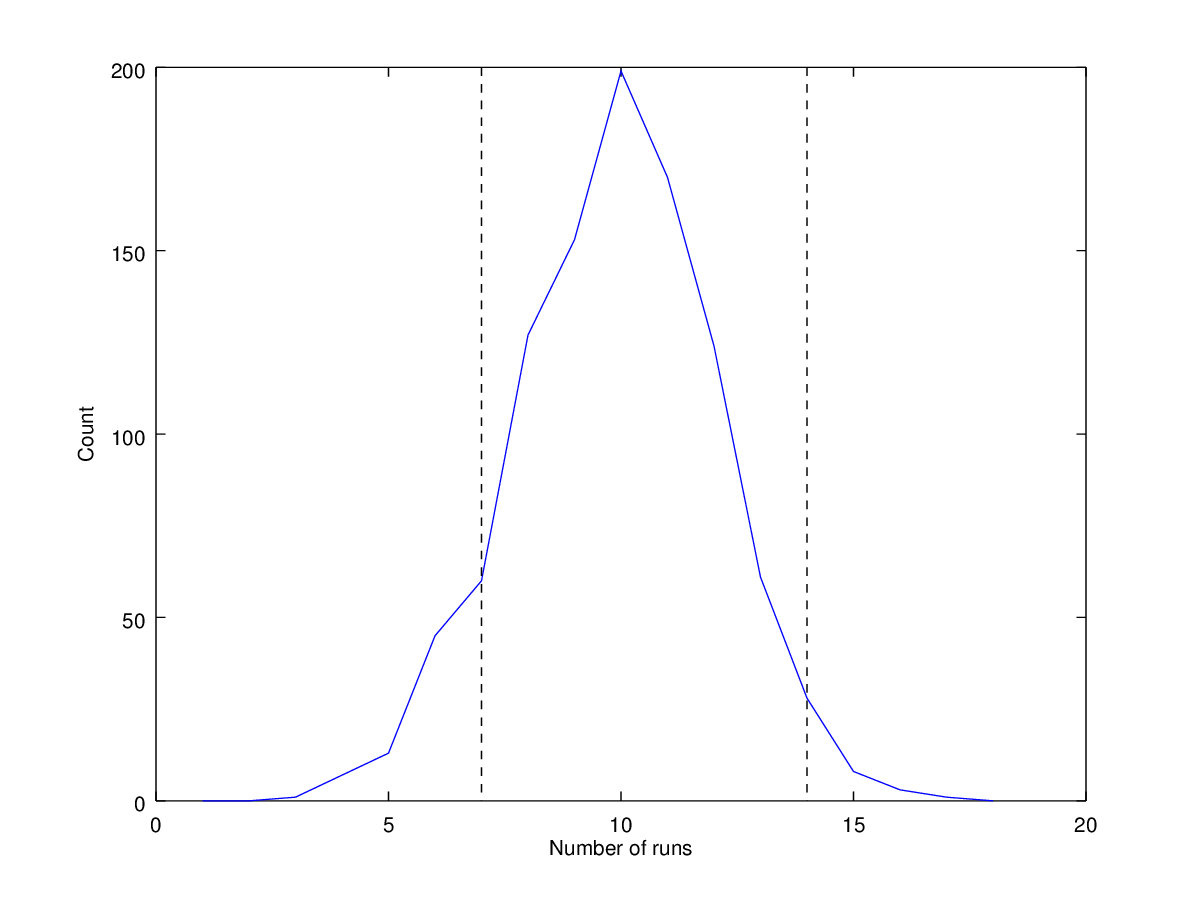
\includegraphics[width=.8\linewidth]{runsTestPlot}
    \begin{tikzpicture}[gnuplot]
%% generated with GNUPLOT 5.0p3 (Lua 5.3; terminal rev. 99, script rev. 100)
%% Mon 02 May 2016 09:54:30 BST
\path (0.000,0.000) rectangle (12.000,9.000);
\gpcolor{color=gp lt color border}
\gpsetlinetype{gp lt border}
\gpsetdashtype{gp dt solid}
\gpsetlinewidth{1.00}
\draw[gp path] (1.688,0.985)--(1.868,0.985);
\draw[gp path] (11.447,0.985)--(11.267,0.985);
\node[gp node right] at (1.504,0.985) {\footnotesize 0};
\draw[gp path] (1.688,2.723)--(1.868,2.723);
\draw[gp path] (11.447,2.723)--(11.267,2.723);
\node[gp node right] at (1.504,2.723) {\footnotesize 50};
\draw[gp path] (1.688,4.460)--(1.868,4.460);
\draw[gp path] (11.447,4.460)--(11.267,4.460);
\node[gp node right] at (1.504,4.460) {\footnotesize 100};
\draw[gp path] (1.688,6.198)--(1.868,6.198);
\draw[gp path] (11.447,6.198)--(11.267,6.198);
\node[gp node right] at (1.504,6.198) {\footnotesize 150};
\draw[gp path] (1.688,7.936)--(1.868,7.936);
\draw[gp path] (11.447,7.936)--(11.267,7.936);
\node[gp node right] at (1.504,7.936) {\footnotesize 200};
\draw[gp path] (1.688,0.985)--(1.688,1.165);
\draw[gp path] (1.688,8.631)--(1.688,8.451);
\node[gp node center] at (1.688,0.677) {\footnotesize 0};
\draw[gp path] (2.772,0.985)--(2.772,1.165);
\draw[gp path] (2.772,8.631)--(2.772,8.451);
\node[gp node center] at (2.772,0.677) {\footnotesize 2};
\draw[gp path] (3.857,0.985)--(3.857,1.165);
\draw[gp path] (3.857,8.631)--(3.857,8.451);
\node[gp node center] at (3.857,0.677) {\footnotesize 4};
\draw[gp path] (4.941,0.985)--(4.941,1.165);
\draw[gp path] (4.941,8.631)--(4.941,8.451);
\node[gp node center] at (4.941,0.677) {\footnotesize 6};
\draw[gp path] (6.025,0.985)--(6.025,1.165);
\draw[gp path] (6.025,8.631)--(6.025,8.451);
\node[gp node center] at (6.025,0.677) {\footnotesize 8};
\draw[gp path] (7.110,0.985)--(7.110,1.165);
\draw[gp path] (7.110,8.631)--(7.110,8.451);
\node[gp node center] at (7.110,0.677) {\footnotesize 10};
\draw[gp path] (8.194,0.985)--(8.194,1.165);
\draw[gp path] (8.194,8.631)--(8.194,8.451);
\node[gp node center] at (8.194,0.677) {\footnotesize 12};
\draw[gp path] (9.278,0.985)--(9.278,1.165);
\draw[gp path] (9.278,8.631)--(9.278,8.451);
\node[gp node center] at (9.278,0.677) {\footnotesize 14};
\draw[gp path] (10.363,0.985)--(10.363,1.165);
\draw[gp path] (10.363,8.631)--(10.363,8.451);
\node[gp node center] at (10.363,0.677) {\footnotesize 16};
\draw[gp path] (11.447,0.985)--(11.447,1.165);
\draw[gp path] (11.447,8.631)--(11.447,8.451);
\node[gp node center] at (11.447,0.677) {\footnotesize 18};
\draw[gp path] (1.688,8.631)--(1.688,0.985)--(11.447,0.985)--(11.447,8.631)--cycle;
\gpcolor{rgb color={0.000,0.000,0.000}}
\gpsetdashtype{gp dt 2}
\draw[gp path](5.483,0.985)--(5.483,8.631);
\draw[gp path](9.278,0.985)--(9.278,8.631);
\gpcolor{color=gp lt color border}
\node[gp node center,rotate=-270] at (0.246,4.808) {\footnotesize Count};
\node[gp node center] at (6.567,0.215) {\footnotesize Number of runs};
\gpcolor{rgb color={0.580,0.000,0.827}}
\gpsetdashtype{gp dt solid}
\draw[gp path] (2.230,0.985)--(2.772,0.985)--(3.315,1.020)--(3.857,1.228)--(4.399,1.437)%
  --(4.941,2.549)--(5.483,3.070)--(6.025,5.399)--(6.568,6.302)--(7.110,7.901)--(7.652,6.893)%
  --(8.194,5.295)--(8.736,3.105)--(9.278,1.958)--(9.821,1.263)--(10.363,1.089)--(10.905,1.020)%
  --(11.447,0.985);
\gpcolor{color=gp lt color border}
\draw[gp path] (1.688,8.631)--(1.688,0.985)--(11.447,0.985)--(11.447,8.631)--cycle;
%% coordinates of the plot area
\gpdefrectangularnode{gp plot 1}{\pgfpoint{1.688cm}{0.985cm}}{\pgfpoint{11.447cm}{8.631cm}}
\end{tikzpicture}

    \caption{The distribution of the number of runs in 1000 access patterns of length 180. The dashed black lines represent 0.05\% tail cut-offs. 92.2\% of values fall within these bounds, implying that the access patterns were created from a random process.}
    \label{fig:runsTestPlot}
\end{figure}

\chapter{Conclusions}

\section{Results}

I successfully implemented the Path ORAM protocol and demonstrated that my implementation agrees with the theoretical overhead of $O(\log N)$, and that it is a statistically secure implementation. Statelessness and recursion were extensions to the project which made it possible to disconnect from and reconnect to ORAM, which proved invaluable during the evaluation process. I built a functioning file system and a search module on top of this, which completed the end-to-end system that was the aim of the project.

Furthermore, the impact of ORAM on a real-world storage scenario was demonstrated. Using a 4GB ORAM block device, the transfer of 1GB of data took 10s, compared to 2s on the block device alone. Although this represents a decrease in transfer rate of a factor of four, it seems to be a reasonable overhead to ensure the privacy of important data.


\section{Future Work}

There is much work to be done in the field of ORAM. One of the main drawbacks of current schemes is that the size of the ORAM must be determined in advance, and the overhead associated with expanding it is enormous. I would like to investigate the possibility of creating a resizeable version of my implementation.

There are also optimisations that could be performed on this implementation. Along with the interesting optimisations mentioned in the literature, I can see room for analysis and optimisation of this specific implementation using benchmarking to identify code hot-spots.

I would like to perform further analysis to gain a deeper understanding of this implementation. I would like to perform more experiments on the initialisation stage of ORAM to understand how the size of the stash changes during this period. Moreover, I would like to spend time adjusting various parameters, including block size and bucket size, in an attempt to find an optimal set of values.

\section{Lessons Learnt}

This project has taught me many important lessons. Perhaps the most significant of these is time management. Throwing myself into the project during the Michaelmas term and vacation meant that I gave myself a large buffer to ensure any hiccoughs later on did not have severe consequences. Related to this, I learnt that predicting the time that each part of a project will take is very difficult and it is therefore important to be both conservative and realistic about the number of things that might go wrong. I learnt the importance and pleasure of sharing one's work with others through contributing to the Mirage community and being invited to talk about the project at Microsoft Research Cambridge. I would like to thank Markulf Kohlweiss from Microsoft Research for his advice and for giving me the opportunity to present my findings. Finally, I have learnt that it is far better to seek advice at the first sign of trouble, rather than waiting until the next scheduled meeting. The advice of experienced supervisors can turn the seemingly catastrophic into a minor disruption.

%%%%%%%%%%%%%%%%%%%%%%%%%%%%%%%%%%%%%%%%%%%%%%%%%%%%%%%%%%%%%%%%%%%%%
% the bibliography
\addcontentsline{toc}{chapter}{Bibliography}
\bibliography{refs}

%%%%%%%%%%%%%%%%%%%%%%%%%%%%%%%%%%%%%%%%%%%%%%%%%%%%%%%%%%%%%%%%%%%%%
% the appendices
\appendix

\chapter{Project Proposal}

% Note: this file can be compiled on its own, but is also included by
% diss.tex (using the docmute.sty package to ignore the preamble)
\documentclass[12pt,a4paper,twoside]{article}
\usepackage[pdfborder={0 0 0}]{hyperref}
\usepackage[margin=25mm]{geometry}
\usepackage{graphicx}
\begin{document}

\vfil

\centerline{\Large Computer Science Project Proposal}
\vspace{0.4in}
\centerline{\Large Encrypted Keyword Search Using}
\vspace{0.05in}
\centerline{\Large Path ORAM on MirageOS}
\vspace{0.4in}
\centerline{\large R. Horlick, Homerton College}
\vspace{0.3in}
\centerline{\large Originator: Dr N. Sultana}
\vspace{0.3in}
\centerline{\large 23 October 2015}

\vfil


\noindent
{\bf Project Supervisors:} Dr N. Sultana \& Dr R. M. Mortier
\vspace{0.2in}

\noindent
{\bf Director of Studies:} Dr B. Roman
\vspace{0.2in}
\noindent
 
\noindent
{\bf Project Overseers:} Dr M. G. Kuhn \& Prof P. M. Sewell


% Main document

\section*{Introduction and Description of the Work}

% Set the scene - change this so that it mentions that what we want is encrypted search

As the cost of large-scale cloud storage decreases and the rate of data production grows, more and more sensitive data is being stored in the cloud. We, of course, want to encrypt our data, to ward off prying eyes, but this comes at a cost. We can no longer selectively retrieve parts of the data at will. We need some method of searching over encrypted data to find the parts we are interested in.

% Set up the threat model for "honest but curious" adversary

So let us say that Alice has a set of documents that she wants to store on an untrusted server, run by Bob. We'll first assume that Bob is ``honest, but curious'', that is, he will attempt to gather all knowledge that he can without deviating from the protocol. Alice wants to store her documents encrypted, but also wants to search over them without Bob being able to learn either the keywords she is searching for, or the results of any query, the documents that contain the keyword. In order to enable efficient search over the documents, Alice stores an encrypted index on the server along with the documents.

There are a number of schemes in the literature that use symmetric encryption techniques to build a searchable encryption scheme. They rely on the use of a trapdoor generating function, that allows Bob to search over the encrypted index and respond to Alice with the matching line from the encrypted index. Then Alice requests the relevant documents from Bob. Bob has a complete view of the communications channel, but does not have access to the trapdoor generating function. He simply sees a query in the form of trapdoor and then a number of requests for specific documents.

The problem is that these all leak the access pattern, so Bob knows which documents matched any query, even if he doesn't know what they matched. It turns out that this pattern of access can leak large amounts of information. In a study \cite{islam2012access} on an encrypted email repository, up to 80\% of plaintext search queries could be inferred from the access pattern alone! So clearly this a leak worth plugging, but how can we do it? 

% Describe ORAM and mention Path ORAM

One solution to our problem is to use Oblivious Random Access Memory (ORAM), a cryptographic primitive that hides data access patterns. In our case, we move the searching and object retrieval functionality back to the client. That is, we turn Bob's server into a block device and we attempt to maintain the property that any two sequences of accesses of the form $(operation,address,data)$, that are the same length, have computationally indistinguishable physical access patterns. Bob should have no way of learning what $address$ we are really accessing, and therefore will never know which documents matched a given search query. 

A trivial ORAM algorithm operates by scanning over the whole ORAM and reading/updating only the relevant block, but this has $O(N)$ bandwidth cost, where $N$ is the number of blocks, which is highly impractical for large-scale storage. Luckily, much better algorithms have been proposed. We choose to focus on Path ORAM \cite{stefanov2013path}, because it has only $O(\log N)$ bandwidth cost in the worst case if $B = \Omega(\log^2 N)$, as well as being incredibly simple conceptually.

% Extend the threat model to incorporate malicious adversary and describe integrity protection techniques

Now let's assume that Bob has become malicious, and is modifying our encrypted data. In order to combat this, we can provide integrity verification by treating the ORAM as a Merkle tree, but with data in every node. The details of this scheme are outlined below after Path ORAM has been described further.

So the project is a searchable encrypted object store, with integrity verification. It will provide a simple, name-value pair API, that allows more complex filesystems to be built on top of it. A block diagram of the system is shown in Figure \ref{miragestack}.

%\begin{figure}
%\setlength{\unitlength}{0.75mm}
%\begin{center}
%\begin{picture}(170,70)
%\put(50,60){\framebox(50,10){Object Store}}
%
%\put(100,65){\vector(1,0){20}}
%\put(120,65){\vector(-1,0){20}}
%
%\put(120,60){\framebox(50,10){Indexed Search}}
%
%\multiput(44,55)(4,0){32}{\line(1,0){2}}
%\put(0,54){BLOCK Interface}
%\put(75,60){\vector(0,-1){10}}
%\put(75,50){\vector(0,1){10}}
%
%\put(145,45){\vector(0,1){15}}
%\put(145,45){\vector(-1,0){45}}
%
%\put(50,40){\framebox(50,10){ORAM}}
%
%\multiput(44,35)(4,0){32}{\line(1,0){2}}
%\put(0,34){BLOCK Interface}
%\put(75,40){\vector(0,-1){10}}
%\put(75,30){\vector(0,1){10}}
%
%\put(50,20){\framebox(50,10){Encryption}}
%
%\multiput(44,15)(4,0){32}{\line(1,0){2}}
%\put(0,14){BLOCK Interface}
%\put(75,20){\vector(0,-1){10}}
%\put(75,10){\vector(0,1){10}}
%
%\put(50,0){\framebox(50,10){BLOCK}}
%
%\end{picture}
%\end{center}
%\caption{The Application Stack: We can use any underlying BLOCK implementation and we can add/remove ORAM, Encryption or Search modules as we please}
%\label{miragestack}
%\end{figure}

\setlength{\unitlength}{0.75mm}
\begin{figure}[b]
\begin{center}
\begin{picture}(170,70)
\put(50,60){\framebox(50,10){File System}}

\put(100,65){\vector(1,0){20}}
\put(120,65){\vector(-1,0){20}}

\put(120,60){\framebox(50,10){Indexed Search}}

\multiput(44,55)(4,0){32}{\line(1,0){2}}
\put(0,54){BLOCK Interface}
\put(75,60){\vector(0,-1){10}}
\put(75,50){\vector(0,1){10}}

\put(145,45){\vector(0,1){15}}
\put(145,45){\vector(-1,0){45}}

\put(50,40){\framebox(50,10){ORAM}}

\multiput(44,35)(4,0){32}{\line(1,0){2}}
\put(0,34){BLOCK Interface}
\put(75,40){\vector(0,-1){10}}
\put(75,30){\vector(0,1){10}}

\put(50,20){\framebox(50,10){Encryption}}

\multiput(44,15)(4,0){32}{\line(1,0){2}}
\put(0,14){BLOCK Interface}
\put(75,20){\vector(0,-1){10}}
\put(75,10){\vector(0,1){10}}

\put(50,0){\framebox(50,10){BLOCK}}

\end{picture}
\end{center}
\caption{The application stack: ORAM satisfies MirageOS's \texttt{BLOCK} interace and any underlying \texttt{BLOCK} implementation can be used}
\label{miragestack}
\end{figure}

\section*{Starting Point}

% Explain Mirage (further explanation of Unikernel OS required) and justify its use

MirageOS is a framework, that pulls together a number of libraries and syntax extensions, to provide a lightweight unikernel operating system, that is designed to run on the Xen hypervisor. A unikernel operating system is a single-address space machine image, customised to provide the minimum set of features to run an application. It provides a command line tool for generating the main file, that links together implementations of various parts of the system, and passes them to the unikernel. There are a number of module signatures that define the operation of devices, such as CONSOLE for consoles, ETHIF for ethernet, and most importantly for us BLOCK, for block devices.

I have chosen to use Mirage for a number of reasons. Firstly, it is lightweight and designed to be run in the cloud, meaning that simple cloud services can be built on top of it that fully leverage the ORAM. Secondly, it is written in OCaml, meaning that I can take full advantage of static typing and a rich module system. 

This will allow me to write my implementation of ORAM and Encryption as a pair of functors that take an implementation of Mirage's BLOCK interface and create new BLOCK implementations, augmented with new features. This means that we can add and remove ORAM and Encryption as we like and the Object Store remains agnostic. This is shown in Figure \ref{miragestack}. It also means that we could use any underlying implementation of the BLOCK interface and that it would plug seamlessly into existing programs. There are currently two implementations of the BLOCK interface, one for Unix and one for Xen, and I would like to support both. This abstraction also allows for the use of cloud storage, implemented as a mapping between the BLOCK interface and a cloud provider's RESTful API.

Other OCaml libraries that will be of most use to me include nocrypto, which provides a wide variety of cryptographic tools, Jane Street's Core library, which standardises and optimises many of OCaml's core modules, and LWT, a lightweight cooperative threading library that is used throughout Mirage.

\section*{Substance and Structure of the Project}

\subsection*{Substance}

% Talk about the relative priorities of sections of the program

	% Main focus is ORAM, then we build object store on top of that, finally we implement the actual search module, but make it clear that, that is not the focus
	
	The main focus of this project is the implementation and evaluation of the Path ORAM protocol. Encrypted search is our target domain and as such will be an integral part of the project, but it is the performance and security properties that Path ORAM provides that we are really interested in.

% Describe Path ORAM protocol more clearly

The Path ORAM protocol has three main components: a binary tree, a stash and a position map. The binary tree is the main storage space. Every node in the tree is a bucket, which can contain up to $Z$ blocks. The tree has height $L$, where the tree of height 0 consists only of the root node, and the leaves are at level $L$. The stash is temporary client-side storage, consisting only of a set of blocks waiting to be put back into the tree. The position map associates, with each block ID, an integer between 0 and $2^L-1$. The invariant that the Path ORAM algorithm maintains is that if the position of a block $x$ is $p$, then $x$ is either in some bucket along the path from the root node to the $p^{th}$ leaf, or in the stash. On every access to the tree, a whole path is read into the stash, the accessed block is assigned a new random position and then as many blocks as possible are written back into the same path. The assignment to a random position means that, in any two access to the same block, the paths that are read are statistically independent.

% Describe recursive path oram protocol

We can extend the basic path ORAM algorithm with recursion. That is, calling the data ORAM $ORAM_0$, we store the position map of $ORAM_0$ in a smaller ORAM, $ORAM_1$, and the position map for this in an even smaller ORAM, $ORAM_2$. We can do this until we have a sufficiently small position map on the client. Supposing that we store $\chi$ leaf addresses in each PosMap ORAM, the position for a data block with address $a_0$ is at $a_1 = a_0 / \chi$ in $ORAM_1$, and in general $a_n = a_0 / \chi^n$ for the address in $ORAM_n$. 

% Mention that we want to be able to disconnect from the block device, so we'll need to be able to store the client state on the ORAM as well

There is actually an issue with using Path ORAM in the context of MirageOS and cloud storage. If the Mirage instance crashes, then we lose the client-side state. With no position map, the ORAM becomes useless. To remedy this, we would have to read the entire contents out in one go and then reinsert it, resulting in a large overhead. There are two solutions to this problem: store the client-side state in persistent storage on the client, or upload the state to the server after every access. The second option is preferable, because it separates the ORAM implementation from the client machine. The client-side state is actually $O(\log N)$, so we should be able to store it on the server without increasing our complexity bounds. 

% Talk about adding integrity verification of the ORAM

As mentioned above, we can add integrity verification to Path ORAM by treating it as a Merkle tree. Each node will store a hash of the form $H = (b_1||\cdots||b_n||h_1||h_2)$, where $b_n$ is the $n^{th}$ block stored in the node, and $h_1$ and $h_2$ are the hashes of the left and right children. We always read and write the whole path at a time, so for the read or write of any single node we only have to read or write two hashes. For instance, on write, we calculate the hash of the leaf node, which is then available for calculating the next level hash. So we only have to read the hash of the sibling of the leaf. This pattern is the same all the way up to the root of the tree.

% Discuss the search mechanism

In order to perform searches over our data, we will store along with it an encrypted inverted index. This is a data structure that, for any keyword, list the documents that contain it. The search module will build the index from the object store and then store the index using the object store. It will provide a search function that, given a keyword, will perform a simple scan over the inverted index and return the identifiers of documents that match it.

% Discuss evaluation techniques

\subsection*{Evaluation}

We need to test for functionality. Does the ORAM successfully write data and read it back out? Does the search function return documents correctly? This will consist of fairly trivial tests, writing objects to and from the block device and searching over them. A range of different types of documents will be used, including randomly (pre-)generated ones and entirely non-random ones, from sources such as Project Gutenberg.

We then want to evaluate performance. What is the overhead when we add the ORAM functor? How do recursion and statelessness further affect this? Does this correspond to the theoretical values from the literature? This will use tests similar to the above, but specifically focusing on time and space efficiency. Using the plain Object Store as a baseline, I will add in encryption and ORAM, separately and in combination to try and isolate the effects of each individual module. 

Finally we want to test the security properties of the project. Is there any statistical correlation between access patterns? Do we provide adequate integrity verification? What, if anything, can be inferred about the search queries? Apart from integrity verification, which we can test by simply corrupting the ORAM and making sure that this is detected, the security comes down to the statistical independence of access patterns. If we can show, using statistical methods, that there is no correlation between two sequences of accesses with identical length, then we have security for not just storage, but for search as well, because this is protected by ORAM's security.

\subsection*{Structure}

The project breaks down into the following sub-projects:

\begin{enumerate}

\item Familiarising myself with OCaml, MirageOS and related libraries

\item Implementing the basic Path ORAM functor and testing that it works in place of existing BLOCK device implementations

\item Implementing the Object Store, testing this and further testing ORAM using it

\item Adding recursion and statelessness to ORAM 

\item Implementing and testing the search module

\item Adding the encryption layer

\item Creation of a suite of tests and experiments to evaluate the performance and security properties of each individual component and of the system as a whole

\item Writing the dissertation

\end{enumerate}

\section*{Success Criteria for the Main Result}

\begin{enumerate}
	\item To demonstrate, through well chosen examples, that I have implemented a functionally correct Path ORAM functor with search capabilities
	\item To demonstrate, through well chosen examples, that the implementation has the expected security properties, i.e. keeps access patterns hidden
\end{enumerate}


\section*{Possible Extensions}

There are a number of ways that this project could be extended. By the nature of the modular design, we can perform optimisations at any layer of the system. There have been a large number of optimisations to Path ORAM proposed in the literature, so if I achieve the goals of my main project, including evaluation, ahead of schedule I will examine these and potentially implement some of them.

In particular for Path ORAM, recursion does add an overhead, but we can reduce this overhead by exploiting locality. Assuming that programs will access adjacent data blocks, we can cache PosMap blocks in a PosMap Lookaside Buffer, so that if all $\chi$ data blocks that are referenced in a PosMap block are accessed in turn we only need to do the recursion once. Doing this na\"ively, however, breaks security, because we are revealing information through the cache hit pattern. To avoid this we use Unified ORAM, which combines all of the recursive ORAMs into a single logical tree. We then use the address space to separate the levels of recursion, so addresses 1 to $N$ are for data blocks, $N + 1$ to $N + (N / \chi)$ for $ORAM_1$ and so on. Now all accesses occur in the same tree, and the security of Path ORAM keeps the cache miss pattern hidden.

Another optimisation compresses the PosMaps, reducing the number of levels of recursion required to achieve the desired client side storage, resulting in an asymptotic bandwidth complexity decrease for ORAM with small block size.

The last two optimisations were originally designed and tested in a secure processor setting \cite{ren2014unified}, so their application to the cloud storage setting is novel.

Another area that could be addressed is the limitation of Path ORAM (and other tree based ORAMs) to fixed-sized trees. We either need to know our storage requirements before setting up the ORAM, potentially wasting resources, or resize them in the na\"ive way as storage requirements increase. Resizability has been implemented for the ORAM construction of \emph{Shi et al.} \cite{shi2011oblivious} in \cite{moataz2015resizable}, but exploring the possibility of making Path ORAM resizable was left as an open research topic.

\section*{Timetable: Work plan and Milestones}

Planned starting date is 16/10/2015.

\begin{enumerate}

\item {\bf 16/10/15 -- 26/10/15} Familiarise myself with relevant Mirage libraries. Implement basic Path ORAM functor.

\item {\bf 27/10/15 -- 09/11/15} Implement basic test harness. Start implementation of object store.

\item {\bf 10/11/15 -- 23/11/15} Finish object store and use it to build more complex tests of the ORAM.

\item {\bf 24/11/15 -- 04/12/15} Add recursion and statelessness to the ORAM.

\item {\bf 05/12/15 -- 18/12/15} Write up implementation section of the dissertation for all parts completed so far.

\item {\bf 18/12/15 -- 31/12/15} Write the search module and design tests for it.

\item {\bf 01/01/16 -- 08/01/16} Write implementation section for the search module.

\item {\bf 09/01/16 -- 29/01/16} Evaluate the project in its current state, achieving an acceptably complete project. Write the progress report.

\item {\bf 30/01/16 -- 08/02/16} Write up the evaluation of the project so far.

\item {\bf 09/02/16 -- 21/02/16} Incorporate encryption model and perform further evaluation using this.

\item {\bf 22/02/16 -- 06/03/16} Submit first draft to supervisors for feedback and modify based on feedback.

\item {\bf 07/03/16 -- 11/03/16} Perform further evaluation and refinement as necessary

\item {\bf 12/03/16 -- 25/03/16} Write final draft of dissertation and then leave it until submission time, in order to focus on revision.

\item {\bf 01/05/16 -- 13/05/16} Reread and make any final edits and then submit.

\end{enumerate}

\section*{Resources Required}

\begin{itemize}

	\item My own laptop for implementation and testing

	\item My own external hard disk for backups

	\item GitHub for version control and backup storage

	\item MirageOS libraries as a basis for the project

\end{itemize}

\end{document}


\end{document}
